\documentclass[12pt,a4paper,pdftex]{article}

% Sprache
\usepackage[ngerman]{babel}
\usepackage[utf8]{inputenc}

\usepackage{graphicx}

% Page layout
\usepackage{geometry}
\geometry{a4paper,lmargin={2.5cm}, rmargin={2.5cm}, tmargin={2cm}, bmargin={2.5cm}}

% Figure and Caption layout
\usepackage[bf]{caption}
\usepackage{subcaption}
\usepackage{wrapfig}
\usepackage{setspace}

% ABB. Verzeichnis (mehr Abstand zw. nummer und titel)
\usepackage{tocloft}
\setlength{\cftfignumwidth}{1.2cm}
\setlength{\cfttabnumwidth}{1.2cm}

% Befehle zur Textauszeichnung (hervorheben, unterstreichen ect.)
\usepackage{color,soul}
\usepackage{xcolor} % bunter Text

% Zitier-Style für Bücher und URL
\usepackage[numbers]{natbib}
\usepackage[breaklinks=true,bookmarks=true,bookmarksopen=true,colorlinks=true,citecolor=black,linkcolor=black,urlcolor=gray,pdfpagemode=UseNone,pdfstartview=FitH]{hyperref}


\usepackage{float}
\usepackage{gensymb}
\usepackage{siunitx}
\usepackage{tabularx}
\usepackage{amsmath}

% für chemische zeichen
\usepackage[version=4]{mhchem}
\usepackage{upgreek}

% for commenting a whole section
\usepackage{verbatim}

\usepackage{pgfgantt}
\usepackage{afterpage}

% Index
\usepackage{imakeidx}
\makeindex[intoc, columnseprule, options= -s indexformat.ist]
\newcommand{\indextitle}{\section{Index}}

% Bilder importieren
\usepackage{epstopdf}
\epstopdfDeclareGraphicsRule{.pdf}{png}{.png}{convert #1 \OutputFile}
\DeclareGraphicsExtensions{.png,.pdf}

% Bildernummerierung fuer jedes kapitel
\usepackage{chngcntr}
\counterwithin{figure}{section}
\counterwithin{table}{section}

% ich hab keine ahnung was die tun und wir brauchen sie auch nicht
%\newcommand{\command}[1]{\texttt{#1}}
%\newcommand{\fileextension}[1]{\texttt{#1}}

% plus minus zeichen
\newcommand{\rpm}{\raisebox{.2ex}{$\scriptstyle\pm$} }

% kapitel title auf deutsch
% \renewcommand{\bibsection}{\section{Literaturverzeichnis}}



%%%%%%%%%%%%%%%%%%%%%%%%%%%%%%%%%%%%%%%%%%%%%%%%%%%%%%%%%%%%%

\begin{document}
\setlength{\parindent}{0pt}

%%%%%%%%%%%%%%%%%%%%%%%%%%%%%%%%%%%%%%%%%%%%%%%%%%%%%%%%%%%%%
% Titelseite
%%%%%%%%%%%%%%%%%%%%%%%%%%%%%%%%%%%%%%%%%%%%%%%%%%%%%%%%%%%%%

\begin{titlepage}
 \begin{center}
        \vspace*{1cm}
        \LARGE
        \textbf{Kurzes Lehrbuch der Neuroanatomie des Säugers}
        \vspace{2cm}
        
        \Large
        Praktikumsprotokoll des Mastermoduls Neuroanatomie
        \vspace{4cm}
        
        \large
        vorgelegt von \\ Jacqueline Laura Göbl, Julia Grüb und Laura Elisa Seidler % Author name
        \vfill
        \large     
        T\"ubingen, \today
    \end{center}
    \newpage
        \thispagestyle{empty}
        \mbox{}
        \newpage
\end{titlepage}


\thispagestyle{empty}
\mbox{}

%%%%%%%%%%%%%%%%%%%%%%%%%%%%%%%%%%%%%%%%%%%%%%%%%%%%%%%%%%%%%% Inhaltsverzeichnis, Tabellen- und Abbildungsverzeichnis
%%%%%%%%%%%%%%%%%%%%%%%%%%%%%%%%%%%%%%%%%%%%%%%%%%%%%%%%%%%%%

\tableofcontents
\newpage
\listoffigures
\listoftables

%%%%%%%%%%%%%%%%%%%%%%%%%%%%%%%%%%%%%%%%%%%%%%%%%%%%%%%%%%%%%
% Textbeginn
%%%%%%%%%%%%%%%%%%%%%%%%%%%%%%%%%%%%%%%%%%%%%%%%%%%%%%%%%%%%%

%_________________ALLGEMEINER_ABSCHNITT______________________

\newpage
\section{Einleitung}
%%%%%%%%%%%%%%%%%%%%%%%%%%%%%%%%%%%%%%%%%%%%%%%%%%%%%%%%%%%%%

 Das Nervensystem ist das wohl komplizierteste System des menschlichen Körpers. Die Funktionsweise dieses komplizierten Kommunikationssystems ist bis heute nicht gänzlich erforscht. Jedoch können durch andauernde Forschung immer mehr Kenntnisse gewonnen werden. Die funktionelle Untereinheit des Nervensystems ist die Nervenzellen. Diese Nervenzellen oder Neurone sind in der Lage Informationen elektrisch oder chemisch an andere Nervenzellen oder nachfolgende Strukturen zu übertragen. Das Nervensystem des Menschen ist aus knapp über tausend Nervenzellen aufgebaut, die ein verzweigtes Netzwerk bilden \textsuperscript{\cite[1]{trepel2011neuroanatomie}}. Die Großhirnrinde des menschlichen Gehirns, als Teil des Nervensystems, kann aufgrund lokaler, histologischer Charakteristika, wie beispielsweise unterschiedliche Schichtung verschiedener Neuronen-Typen, in 52 voneinander abgrenzbare Areale, die sogenannten \textbf{Brodmann-Areale}\index{Brodmann-Areale}, unterteilt werden (Abb.~\ref{fig:brodmann_areale}). Obwohl diese Areale bereits Anfang des zwanzigsten Jahrhunderts definiert wurden, dienen sie bis heute zur Beschreibung distinkter Hirnareale. So ist das Brodmann-Areal 17 heute mit der primären Sehrinde, das Areal 41 mit der primären Hörrinde gleichzusetzen. Das Brodmann-Areal 6, sowie Teile des Areals 8, beschreiben den prämotorischen Cortex \textsuperscript{\cite[9]{trepel2011neuroanatomie}}. Die Beständigkeit der von Brodmann festgelegten Areale dienen als Beispiel des Zusammenspiels von Morphologie und Funktion funktioneller Systeme. Sie zeigen, dass die Struktur des Systems die Grundlage der zugehörigen Funktion ist.

\begin{figure}[H]
    \centering
    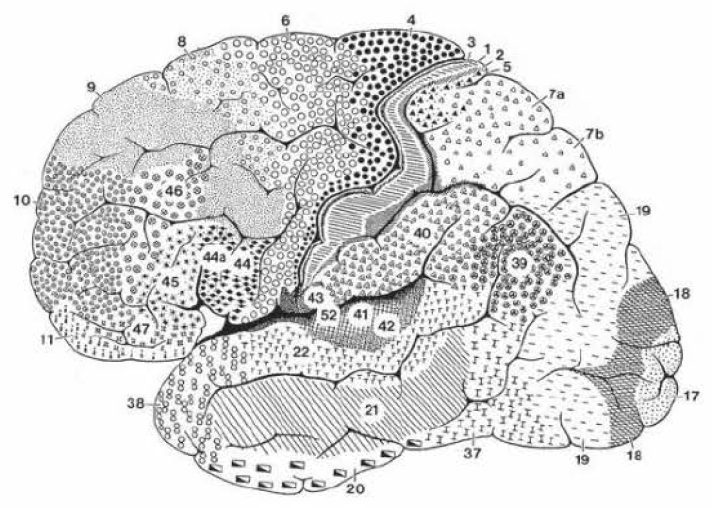
\includegraphics[width=0.7\textwidth]{pictures/Bilder_Jule/Andere/brodmann.PNG}
    \caption[Brodmann-Areale]{\textbf{Brodmann-Areale.} Die Großhirnrinde wurde durch Brodmann, aufgrund histologischer Merkmale, in 52 Areale unterteilt. \\
    Abbildung aus \textit{Neuroanatomie}, Trepel \textsuperscript{\cite[9]{trepel2011neuroanatomie}}.}
    \label{fig:brodmann_areale}
\end{figure}

Um die zugrundeliegende Struktur des Nervensystems, bzw. des Gehirns, besser beschreiben zu können, werden unterschiedliche Ebenen herangezogen (Abb.~\ref{fig:schnittebenen}). Die rostro-caudale Achse beschreibt die Achse zwischen Kopf (rostral) und Schwanz (caudal) eines Tieres, die dorso-ventrale Achse die zwischen Rücken (dorsal, posterior) und Bauch (ventral, anterior). In Bezug auf das Gehirn kann, vor allem beim Menschen, noch zwischen oben (superior) und unten (inferior) unterschieden werden. Des Weiteren existieren drei verschiedene (Schnitt-)Ebenen: die Horizontal-, Sagittal- und Coronal-Ebene \textsuperscript{\cite[15]{kandel2013principles}}. Ziel dieses Protokolls ist es, einen groben Überblick über die grundlegende funktionelle Anatomie des Gehirns zu geben. Es soll ein Verständnis der räumlichen Lage der unterschiedlichen Areale und funktionellen Systeme entstehen. Die wichtigsten funktionellen Untereinheiten, sowie die sensorischen und motorischen Bahnen, die integrativen Systeme und die generellen Transmittersysteme sollen genauer beschrieben werden.

\begin{figure}[H]
    \centering
    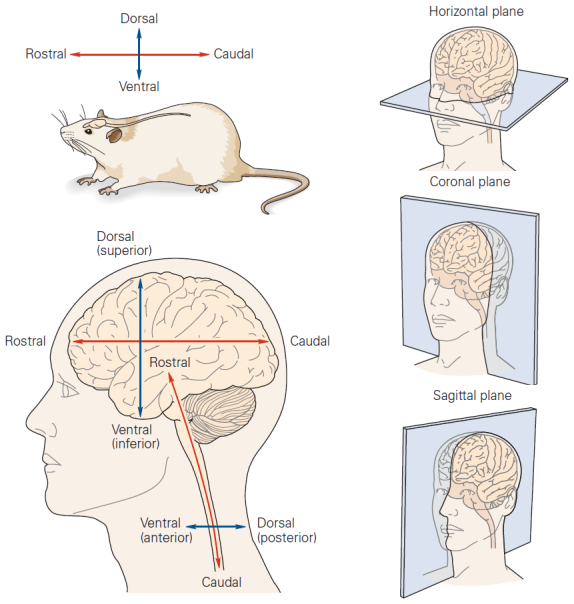
\includegraphics[width=0.7\textwidth]{pictures/Bilder_Jule/Andere/Schnittebenen.png}
    \caption[Achsen und Schnittebenen]{\textbf{Achsen und Schnittebenen.}\\
    Abbildung aus \textit{Principles  of Neural Science}, Kandel et al. \textsuperscript{\cite[15]{kandel2013principles}}.}
    \label{fig:schnittebenen}
\end{figure}{}


\newpage
\section{Material und Methoden}
%%%%%%%%%%%%%%%%%%%%%%%%%%%%%%%%%%%%%%%%%%%%%%%%%%%%%%%%%%%%%

\subsection{Perfusion der Ratte}
%%%%%%%%%%%%%%%%%%%%%%%%%%%%%%%%%

Beim Versuchstier handelte es sich um eine 280~g schwere, weibliche Spraque-Dawley-Ratte. Diese wurde mittels 0.84~ml Narcoren (0.3~ml/100~g, 16~\% Babiturat) narkotisiert. Das Narkotikum wurde im 45\degree~Winkel in den unteren Bauchraum (intraperitoneal) injiziert. Die Dosis stellt für das Tier eine starke Überdosis dar, die nach einiger Zeit zum Herzstillstand führt. Nach der Injektion folgte eine kurze Ruhephase für das Tier. Da das Versuchstier nach 5:50 Minuten Ruhephase nicht narkotisiert war, wurden weitere 0.3~ml Narcoren, ein Drittel der ursprünglichen Dosis, injiziert. Nach weiteren 3:20 Minuten, nach dem das Tier vollständig narkotisiert war und keinen Zwischensehnenreflex mehr zeigte, wurde mit der \textbf{Perfusion} begonnen (Abb.~\ref{fig:perfusion}). Dafür wurde zunächst der Thorax geöffnet, um das noch schlagende Herz freizulegen. Die Haut wurde vorsichtig mittig des Bauches von caudal nach rostral geöffnet. Anschließend wurde das Zwerchfell entlang des Rippenbogens aufgetrennt. Das Herzbändchen, sowie die Rippen auf der linken und rechten Seite, wurden durchtrennt. Sobald das Herz freigelegt war, konnte mittels Spritze die linke Herzkammer geöffnet werden um eine Perfusionskanüle (Oliven-Kanüle) einzuführen. Diese wurde mit einer Klemme befestigt. Danach wurde die rechte Herzvorkammer mit einem Schnitt geöffnet. Mit etwa 150~ml 0.01m~PBS (Phosphate-buffered Saline, Raumtemperatur) wurde das Herz-Kreislauf-System unter Verwendung einer Schlauchpumpe vorgespült. Dass sämtliches Blut ausgewaschen ist, ist am blass werdenden Gewebe sichtbar. Bei Ratten mit roten Augen ist dies am Farbwechsel der Augen von rot zu weiß erkennbar. Als dies geschehen war, konnte das Gewebe mittels 350~ml 4~\%igem, eiskaltem Paraformaldehyd fixiert werden. Durch chemische Reaktionen in den Muskeln kann es dabei zu Muskelzuckungen kommen. Die ausreichende Fixierung des Gewebes ist an einer stabilen Kopfposition beim Anheben des Tieres zu erkennen.

\begin{figure}[H]
    \centering
    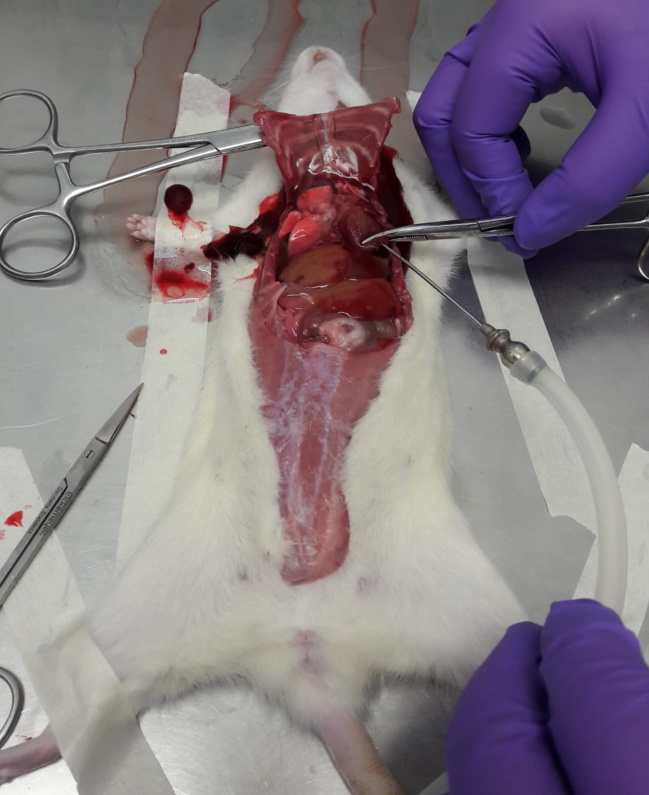
\includegraphics[width=0.45\textwidth]{pictures/Bilder_Jule/Ratte/perfusion.png}
    \caption[Perfusion der Ratte]{\textbf{Perfusion der Ratte.} Der Brustkorb des Tieres ist nach oben hin geöffnet. Mittels Kanüle wird das Blut aus dem Herz-Kreislauf-System gespült.}
    \label{fig:perfusion}
\end{figure}

Nach der Fixierung folgte die \textbf{Gehirnentnahme}. Dazu wurde der Kopf des Tieres abgetrennt. Anschließend wurde die Haut dorsal, entlang der Mittellinie, aufgetrennt. Die die Wirbelsäule umgebene Nackenmuskulatur wurde entfernt. Mit einem Rangeur wurde der Schädelknochen vorsichtig von caudal nach rostral entfernt, bis das Gehirn vollständig freigelegt war. Nachdem alle Knochenrückstände vollständig entfernt wurden, konnte das Gehirn nachfixiert werden. Zur \textbf{Nachfixierung} wurde das Gehirn über Nacht in 4~\%iges Paraformaldehyd gegeben.

\subsection{Färbungen des Gewebes}
%%%%%%%%%%%%%%%%%%%%%%%%%%%%%%%%%%%

In Vorbereitung auf die Färbungen muss das Gehirn in dünne Scheiben geschnitten werden. Um Gewebeschädigungen durch den dazu erforderlichen Gefriervorgang zu vermeiden, ist ein \textbf{Gefrierschutz} erforderlich. Dafür wurde das Gehirn in 20~\%ige Sucroselösung, bestehend aus 20~g Zucker gelöst in jeweils 70~ml Phosphatpuffer, aufgefüllt auf 100~ml, gelegt. Innerhalb dieser Lösung wurde das Gehirn solange aufbewahrt, bis es auf den Boden abgesunken war. War dies geschehen, wurde der Vorgang mit 30~\%iger Sucroselösung wiederholt. Da dies einen Tag dauern kann, wurde das Gehirn über das Wochenende in der Lösung gelassen. Zum \textbf{Schneiden} des Gehirns wurde ein Gefriermikrotom verwendet. Um eine bessere Orientierung zu ermöglichen, wurde eine Seite des Cortex mit einem länglichen Schnitt entlang der rostro-caudalen Achse gekennzeichnet. Anschließend wurde das Gehirn in 50~$\upmu$m dicke Scheiben geschnitten, die bis zum Färbevorgang einzeln in mit TBS (Tris-buffered Saline) befüllten Mikroplates, im Kühlschrank, aufbewahrt wurden. Bei jedem dritten Schritt kam eine unterschiedliche Färbemethode zum Einsatz. Für die Nissl- und Faser-Färbung wurden jeweils vier Schnitte, in der richtigen Reihenfolge, auf Gelatine Chromalaun beschichteten Objektträgern aufgezogen. Nachdem die Schnitte auf den Objektträgern getrocknet waren, konnte mit dem Färbevorgang begonnen werden. Die mittels immunhistochemischen Nachweises gefärbten Schnitte wurden für den Färbevorgang in zwei Gruppen, a und b, eingeteilt. Dabei wurde jeder zweite Schnitt derselben Gruppe zugeteilt. Erst nach der Färbung wurden die unterschiedlichen Gruppen auf die Objektträger aufgezogen. In den folgenden Abschnitten des Protokolls sind verschiedene, mikroskopische Aufnahmen des gefärbten Gewebes dargestellt. Die \textbf{Namensgebung der Schnitte} setzt sich dabei wie folgt zusammen: Der erste Buchstabe gibt die Färbung an (N: Nissl, F: Faser, I: Immunhistochemisch). Die darauf folgende Zahl beschreibt die Nummer des Objektträgers. Dabei wurden die Schnitte von caudal nach rostral (1-32) aufgezogen. Nach einem Trennstrich folgt die Nummer (1-4) des sich auf dem Objektträger befindenden Schnittes.

\subsubsection{Nissl-Färbung}
%%%%%%%%%%%%%%%%%%%%%%%%%%%%%%

Mittels Nissl-Färbung können Nucleinsäuren, die in den Somata der Zellen enthalten sind, angefärbt werden. In Vorbereitung auf die Nissl-Färbung wurde eine \textbf{Thioninstammlösung} angesetzt. Für diese wurde 1~g Thionin in 10~ml 100~\%igem Alkohol gelöst. Nach 30~min wurden 500~ml destilliertes Wasser hinzu gegeben. Diese Lösung wurde vorsichtig, ohne sie zum Kochen zu bringen, erwärmt. Nach dem sie abgekühlt war und gefiltert wurde, konnte aus der Stammlösung eine Gebrauchslösung gemischt werden. Diese \textbf{Thioningebrauchslösung} bestand aus einer filtrierten Lösung aus 100~ml der Stammlösung, gemischt mit 100~ml destilliertem Wasser. Vor Beginn der Färbung wurden die gut getrockneten Schnitte auf den Objektträgern für 3~min in PBS gegeben. Im Anschluss konnte mit der \textbf{Färbung} begonnen werden. Dafür wurden die Schnitte für 1-2~min in frisch gefilterte Thioninlösung gestellt, solange bis die Schnitte leicht überfärbt waren. Anschließend wurden sie kurz mit 0.01m~mPB abgespült. Die Objektträger wurden für jeweils 3~min in eine aufsteigende Alkoholreihe (50~\%, 70~\%, 90~\%) gegeben. Im folgenden Schritt wurde der Färbegrad der Schnitte kontrolliert. Zu stark gefärbte Schnitte wurden in 96~\%igen Alkohol, gemischt mit 5 Tropfen Eisessig, gegeben. Für zu schwach gefärbte Schnitte wurde die Alkoholreihe in umgekehrter Reihenfolge, und anschließend auch die Färbung, wiederholt. Nach dem alle Schnitte den gewünschten Färbegrad erreicht hatten, wurden die Schnitte für 3~min in 96~\%igen Alkohol, dann zweimal für jeweils 5~min in frischen, 100~\%igen Alkohol gegeben. Danach wurden die Schnitte zweimal für jeweils 10~min in (frisches) Xylol gelegt. Im Anschluss wurden die noch nassen Schnitte auf den Objektträgern mittels Entellan eingedeckelt. 

\subsubsection{Faser-Färbung}
%%%%%%%%%%%%%%%%%%%%%%%%%%%%%%%

Die Faser-Färbung wurde mittels \textbf{Goldchloridlösung} (0.2~\%) nach Schmued durchgeführt. Mittels dieser Färbemethode werden myelinisierte Fasern angefärbt. Für die Färbelösung wurden 500~ml 0.02m Phosphatpuffer mit 4.5~g Natriumchlorid und 1~g Goldchlorid gemischt. Mit 1~N Natriumhydroxid wurde die Lösung auf einen pH-Wert zwischen 6.8 und 7.0 gepuffert. Zum \textbf{Färben} wurden die trockenen Objektträger mitsamt den Schnitten in die Goldchloridlösung gestellt. Nach etwa 30~min wurden die Schnitte unter dem Mikroskop kontrolliert. Nach dem die Schnitte ausreichend gefärbt waren, dies kann bis zu 1~h dauern, wurden sie in 0.01m~PBS gespült. Danach wurden die Objektträger für 5~min in 2.5~\%ige Natriumthiosulfatlösung gegeben. Im Anschluss wurden sie dreimal für jeweils 5~min in 0.01m PBS gewaschen. Entwässert wurden die Schnitte anschließend ein einer aufsteigenden Alkoholreihe (50~\%, 70~\%, 90~\%, 96~\%, 100~\%, 100~\%). Danach wurden die entwässerten Gehirnschnitte jeweils für 10~min in (frisches) Xylol gelegt. Im Anschluss wurden sie mit Entellan eingedeckelt.

\subsubsection{Immunhistochemische Färbung}
%%%%%%%%%%%%%%%%%%%%%%%%%%%%%%%%%%%%%%%%%%%%

Die immunhistochemische Färbung dient zum Nachweis catecholaminerger Neurone. Zu den catecholaminergen Stoffen gehören Adrenalin, Noradrenalin, Dopamin, sowie deren Derivate. Alle drei primären Catecholamine werden ausgehend von der Aminosäure Tyrosin synthetisiert \textsuperscript{\cite[13]{kandel2013principles}}. An der Synthese sind fünf Enzyme beteiligt. Eines dieser Enzyme, die Tyrosin-Hydroxylase, dient als Grundlage dieses Nachweises. Es lässt sich im Soma und den in den Axontermini catecholaminerger Nervenzellen auffinden. Um dieses Enzym in Gewebe sichtbar zu machen, wurde hier die sogenannte \textbf{ABC-Methode} angewendet. Dies ist ein indirektes Färbeverfahren, das dopaminerg-aktive Regionen (Catecholamin) erkennbar macht. Dazu wurden zwei unterschiedliche Antikörper verwendet. Zum einen ein primärer Antikörper, der direkt an das Enzym Tyrosin-Hydroxylase bindet und ein sekundärer, biotinylierter Antikörper, der sich wiederum an den primären anheftet. An das biotinylierte Ende des sekundären Antikörpers binden Avidin-Biotin-Complexe, die Meerrettichperoxidase-Moleküle (HRP) enthalten. Wird nun das farblose 3,3'-Diaminobenzidin-Tetrahydrochlorid (DAB) hinzugegeben oxidiert der Komplex zu einem bräunlichem Produkt \textsuperscript{\cite{burry2009immunocytochemistry}}. Die Durchführung des Nachweises kann in mehrere Schritte unterteilt werden. Vor dem ersten Schritt wurden die Schnitte, die sich in Microplates befanden mit TBS Puffer gewaschen. Der erste Schritt der Färbung wird als \textbf{Quenching} bezeichnet. Hierbei wurden die Schnitte in TBS-Puffer zusammen mit 0.3~\%~igem Wasserstoffperoxid (0.3~ml 30~\%~iges H$_{2}$0$_{2}$ in 100~ml PBS) gegeben. Damit sollte eine nicht-spezifische Hintergrundfärbung durch endogene Peroxidasen vermieden werden. Das zugegebene Wasserstoffperoxid stoppt endogene Peroxidasen im Gewebe, die eventuell eine falsch-positive Reaktion mit DAB (letzter Schritt) hervorrufen könnten \textsuperscript{\cite{burry2009immunocytochemistry}}. Anschließend wurden die Schnitte wiederum in TBS gewaschen und es folgte der zweite Schritt, das \textbf{Blocken} unspezifischer Bindungen und die \textbf{Permeabilisierung} der Zellmembran. Dies wurde durch Zugabe eines Blockers bestehend aus 9~ml Goat-Serum und 1~ml Carrier ermöglicht. Der Carrier wiederum setzte sich aus 150~ml TBS, 3~ml Goat-Serum und 2.25~ml 20~\%~igem Triton X zusammen. Um nicht-spezifische Protein-Protein-Interaktion zwischen Antikörpern und Proteinen zu unterbinden, muss sich vor Zugabe des ersten Antikörpers ein blockendes Protein kompetitiv mit den unspezifischen Bindungsstellen verknüpfen. Der Antikörper bindet an die sogenannten \textbf{Fc-Rezeptoren} im Gewebe. Diese sind auf Makrophagen und vielen anderer immunologischen Zellen im Gewebe zu finden und könnten daher jeden Antikörper, der während der Färbung hinzugeben wird, binden. Das Triton-X ist ein nicht-ionisches Tensid und fungiert als Detergent. Seine Zugabe führte zu einer Auflockerung der Zellmembran, sodass die Antikörper in die Zelle eindringen und intrazellulär binden können \textsuperscript{\cite{burry2009immunocytochemistry}}. Nach dem Blocken erfolgte der dritte Schritt mit Zugabe des \textbf{primären Antikörpers}. Dieser bestand aus dem Antikörper r-a-TH (rabbit-anti-Tyrosin-Hydroxylase), der 1:500 mit dem Carrier verdünnt wurde (20~$\upmu$l AK in 9980 ~$\upmu$l Carrier). Der primäre Antikörper besitzt eine \textbf{Fc-Region} und eine \textbf{Fab-Region}. Die Fab-Region des primären Antikörpers bindet an das Epitop der Tyrosin-Hydroxylase \textsuperscript{\cite{burry2009immunocytochemistry}}. Das Gemisch wurde unter ständigem schütteln über Nacht in den Kühlschrank gestellt. Am zweiten Tag wurden die Schnitte zunächst mit TBS-Puffer gewaschen, bevor dann im vierten Schritt der \textbf{sekundäre Antikörper} hinzu gegeben wurde. Der Sekundärantikörper ist biotinyliertes Goat-a-r (Goat-anti-rabbit) das 1:1000 in Carrier gemischt wurde (10~$\upmu$l AK mit 9990~$\upmu$l Carrier). Er bindet mit seiner Fab-Region an die Fc-Region des primären Antikörpers \textsuperscript{\cite{burry2009immunocytochemistry}}. Nach einer Stunde wurde der Rest mit PBS-Puffer ausgewaschen und es erfolgte der fünfte Schritt, die Zugabe des \textbf{Avidin-Biotin-Complex (ABC)}. Das ABC-Kid wurde 30~min zuvor angesetzt und bestand aus  100~$\upmu$l Avidin, 100~$\upmu$l Biotin und 10~ml des Carriers PBN. Dieser Carrier wiederum setzt sich aus 12.5~ml 0.2~M Phosphatpuffer, 7.3~g Natriumclorid und 250~ml destilliertem Wasser zusammen. Am Biotin befinden sich zusätzlich zahlreichen HRP-Moleküle, die sich unter der Zugabe von Avidin in Komplexen anreichern. Dieser Komplex lager sich nun am biotinyliertem Sekundärantikörper an \textsuperscript{\cite{burry2009immunocytochemistry}}. Der restliche ungebundene Antikörper wurde nach 60~min durch waschen in TBS entfernt. Anschließend folgte der letzte Schritt, die \textbf{DAB-Reaktion}, die auch die charakteristische braune \textbf{Färbung} erzeugte. Für diese Reaktion wurden 10~mg DAB mit 20~ml filtriertem TBS gemischt. Kurz vor Gebrauch wurde zusätzlich noch 9~$\upmu$l Wasserstoffperoxid hinzu gegeben. Das farblose DAB wird von der an den AB-Komplex gebundene Meerrettich-Peroxidase (HRP) zu einem braunen Produkt oxidiert \textsuperscript{\cite{burry2009immunocytochemistry}}. Dieser Färbegrad wurde kontinuierlich kontrolliert und als die Schnitte ausreichend gefärbt waren, wurde die Reaktion mit TBS-Puffer gestoppt. Anschließen wurden die Schnitte sortiert, auf Objektträger aufgezogen und über Nacht getrocknet. Am dritten Tag wurden die Schnitte dann zunächst über eine aufsteigende Alkoholreihe (50~\%, 70~\%, 80~\%, 90~\%, 96~\%, 2~x~100~\%) entwässert. Im Anschluss wurden dies Objektträger zweimal für 10~min in (frisches) Xylol gestellt und danach mit Entellan eingedeckelt.  


\subsection{Mikroskopie}
%%%%%%%%%%%%%%%%%%%%%%%%%%%%%%%%%%%%%%%%%%%

Die Bilder der einzelnen Färbungen wurden mit einem Mikroskop der Firma Zeiss aufgenommen und mit dem Programm 'Axio Vision' (AxioVs40 4.8.2.0, Copyright 2006-2010, Carl Zeiss MicroImaging GmBH) an einem Aufnahmecomputer bearbeitet. Mit diesem Programm konnten Panoramabilder erstellt werden und die Quantitative Analyse der Kerngebiete und Zellen des catecholaminergen Systems (Kap.~\ref{sec:immu}) berechnet werden.


%%%%%%%%%%%%%%%%%%%%%%%%%%%%%%%%%%%%%%%%%%%%%%%%%%%%%%%%%%%%%
%%%%%%%%%%%%%%%%%%%%%%%%%%%%%%%%%%%%%%%%%%%%%%%%%%%%%%%%%%%%%

%_____________________JULES_ABSCHNITT________________________

\newpage
\section{Entstehung des Gehirns}
%%%%%%%%%%%%%%%%%%%%%%%%%%%%%%%%%%%%%%%%%%%%%%%%%%%%%%%%%%%%%

\subsection{Neurulation}
\label{subsec:Neurulation} \index{Neurulation}
%%%%%%%%%%%%%%%%%%%%%%%%%%%%%%%%%%%%%%%%%%%%%%%%%%%%%%%

\begin{minipage}[b]{0.68\textwidth}
Der Embryo entwickelt drei Keimblätter: Endoderm, Mesoderm und Ektoderm. Aus diesen werden in späteren Entwicklungsschritten unterschiedliche Gewebe und Organe des adulten Individuums entstehen. Aus dem Mesoderm entstehen Skelett-, Muskel- und Bindegewebe, aus dem Endoderm Verdauungs-, Atem- und Urogenitaltrakt. Aus dem Ektoderm entstehen später die Haut und das Nervensystem \textsuperscript{\cite[1]{crossman2014neuroanatomy}}. Die Entwicklung des Nervensystems beginnt mit der Neuralinduktion. Durch einen Anreiz des Mesoderms und der Chorda dorsalis bildet das darüber liegende Ektoderm das sogenannte Neuroektoderm aus. Das Neuroektoderm bildet dann die Neuralplatte (Abb.~\ref{fig:neurulation}). Im Laufe der Neurulation senkt sich diese in Richtung des Mesoderms ab und bildet so die Neuralrinne. Die angrenzenden Strukturen werden dadurch leicht erhöht und bilden die Neuralfalten. Durch weiteres Absinken und Abschnüren entsteht aus der Neuralrinne schließlich das Neuralrohr, aus den Neuralfalten die Neuralleisten. Aus der \textbf{Neuralleiste} werden im späteren Verlauf die Strukturen des peripheren Nervensystems entstehen. Aus dem \textbf{Neuralrohr} entwickelt sich das zentrale Nervensystem. Im Bereich des Kopfes bildet es das Gehirn aus, im hinteren Rumpfabschnitt das Rückenmark. Aus dem Hohlraum, den das Neuralrohr umschließt, entsteht das Ventrikelsystem\index{Ventrikelsystem} \textsuperscript{\cite[1]{trepel2011neuroanatomie}}.
\end{minipage} \hspace{0.1cm}
\begin{minipage}[b]{0.3\textwidth}
\begin{figure}[H]
    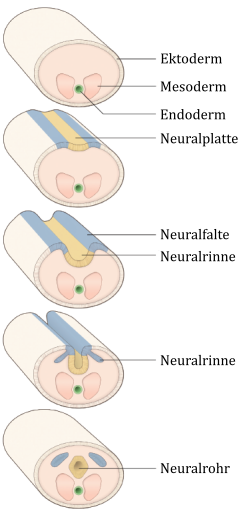
\includegraphics[width=\textwidth]{pictures/Bilder_Jule/Andere/Neurulation_crossm1.png}
    \caption[Neurulation]{\textbf{\\Neurulation.}\\
    Abbildung aus \textit{Neuroanatomy}, Crossman und Neary \textsuperscript{\cite[1]{crossman2014neuroanatomy}}.}
    \label{fig:neurulation}
    \end{figure}    
\end{minipage} 

\subsection{Cephalisation}
\label{subsec:Cephalisation} \index{Cephalisation}
%%%%%%%%%%%%%%%%%%%%%%%%%%%%%%%%%%%%%%%%%%%%%%%%%%%%%%%
Zentrales und Peripheres Nervensystem der Wirbeltiere werden von unterschiedlichen ontogenetischen Strukturen gebildet. Das Periphere Nervensystem (PNS) wird aus Zellen der mesodermalen Neuralleiste gebildet. Im Gegensatz dazu wird das Zentrale Nervensystem (ZNS), das sowohl Gehirn als auch Rückenmark umfasst, von den Zellen des Neuralrohrs gebildet. Somit ist das ZNS ektodermalen Ursprungs. \\

\begin{figure}[H]
\centering
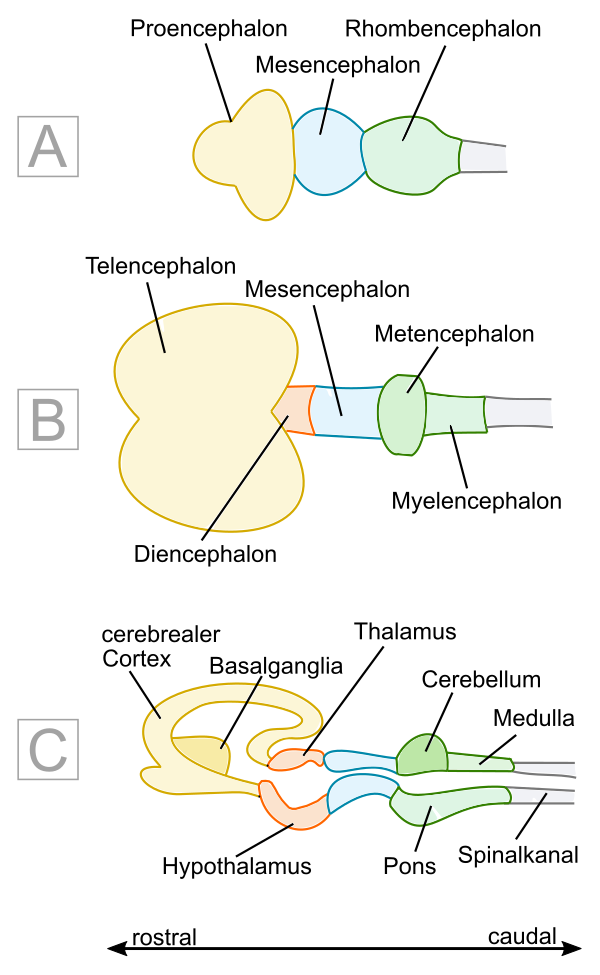
\includegraphics[width=0.5\textwidth]{pictures/Bilder_Jule/Andere/cephalisation.png}
\caption[Grundgliederung des Säugerhirns]{\textbf{Grundgliederung des Säugerhirns.} \textbf{A}:~primäre Hirnbläschen (3), \textbf{B}:~sekundäre Hirnbläschen (5), \textbf{C}:~Grundgliederung und Ventrikelsystem. \\
Abbildung nach \textit{Neurowissenschaften}, Bear et al. \textsuperscript{\cite[7]{neurowissenschaften_baer}}.}
\label{fig:cephalisation}
\end{figure}

\noindent Im Laufe der Cephalisation bildet das frühe Neuralrohr rostral drei Schwellungen aus. Diese dehnen sich zunehmend aus und bilden die primären Hirnbläschen: Das Vorderhirn (Proencephalon)\index{Proencephalon}, Mittelhirn (Mesencephalon) und Rautenhirn (Rhombencephalon)\index{Rhombencephalon} (Abb.~\ref{fig:cephalisation}~A). Diese entwickeln sich im Laufe der Gehirnentwicklung zu den fünf sekundären Hirnbläschen: Das Proencephalon bildet zwei laterale Fortsätze aus, die cerebralen Vesikel, die später die Hemisphären des cerebralen Cortex bilden werden. Zusammen mit dem rostralen Vorderhirn bilden sie das Endhirn (\textbf{Telencephalon})\index{Telencephalon}. Der caudale Teil des Vorderhirns bildet das Zwischenhirn (\textbf{Diencephalon})\index{Diencephalon}, aus dem Thalamus und Hypothalamus gebildet werden. Das Mittelhirn (\textbf{Mesencephalon})\index{Mesencephalon} formt vier Schwellungen, die zum inferioren und superioren Colliculus heranwachsen. Das Rautenhirn gliedert sich in Hinterhirn (\textbf{Metencephalon})\index{Metencephalon} und Nachhirn (\textbf{Myelencephalon})\index{Myelencephalon} auf, die später Pons und Cerebellum (Metencephalon), beziehungsweise die Medulla (Myelencephalon) bilden (Abb.~\ref{fig:cephalisation}~C). Zusammengefasst ist das Vertebratengehirn am Ende der Cephalisation in vier Teilbereiche gegliedert; Das Telencephalon, Diencephalon, Mesencephalon und das Rhombencephalon, das Met- und Myelencephalon zusammenfasst (Abb.~\ref{fig:cephalisation}~B) \textsuperscript{\cite[10]{watson2010thebrain}}.

\subsection{Das Ventrikelsystem}
\label{subsec:} \index{Ventrikelsystem}
%%%%%%%%%%%%%%%%%%%%%%%%%%%%%%%%%%%%%%%%%%%%%%%%%%%%%%%

Jedes dieser Hirnvesikel umhüllt dabei einen mit Hirnwasser (\textit{Liquor cerebrospinalis}) gefüllten Hohlraum. Diese miteinander in Verbindung stehenden Ventrikel bilden das Ventrikelsystem (Abb.~\ref{fig:ventrikelsystem}), das auch als innerer Liquorraum  bezeichnet wird. Es besteht aus vier Ventrikeln: Zwei laterale Ventrikel, auch Seitenventrikel genannt, befinden sich im Telencephalon. Sie verlaufen entlang des Hippocampus, der ihre mediale Wand bildet. Der dritte Ventrikel befindet sich im Diencephalon. Im Gegensatz zu den lang gezogenen lateralen Ventrikeln befindet sich der dritte Ventrikel spaltförmig in der Midsagittalebene des Gehirns. Das Mesencephalon umgibt das Aquädukt (\textit{Aqueductus cerebri} oder \textit{Aqueductus mesencephali}). Es liegt unter der Vierhügelplatte und über dem Tegmentum. Der vierte und letzte Ventrikel ist im Rhombencephalon lokalisiert und erstreckt sich oberhalb des Hirnstamms und unterhalb des Cerebellums bis hin zum Rückenmark
\textsuperscript{\cite[2]{watson2010thebrain}}.

\begin{figure}[H]
	\centering
	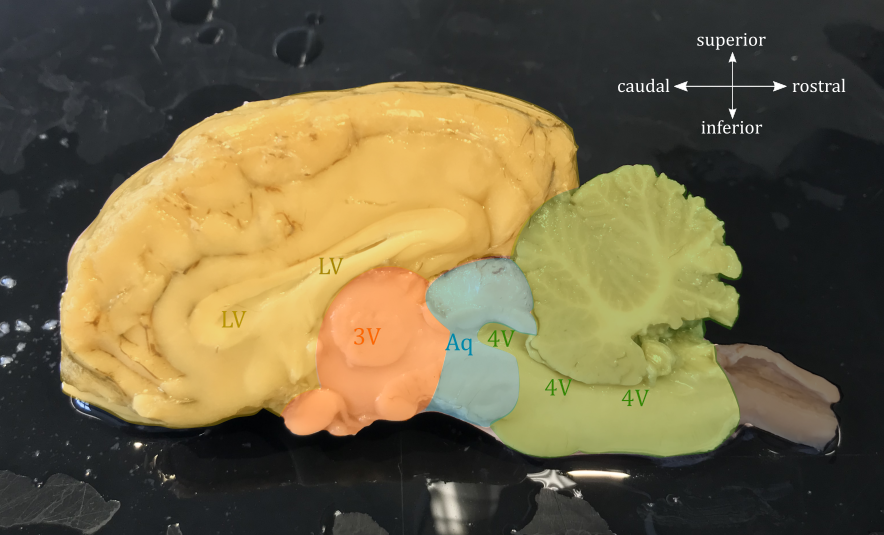
\includegraphics[width=0.8\textwidth]{pictures/Bilder_Jule/Andere/ventrikelsystem.png}
	\caption[Das Ventrikelsystem]{\textbf{Das Ventrikelsystem.} Das Ventrikelsystem im Midsagittalschnitt des Schafhirns. Das Telencephalon und der laterale Ventrikel (LV) sind gelb, Diencephalon und dritter Ventrikel (3V) orange, Mesencephalon und Aquädukt (Aq) blau und Rhombencephalon, sowie vierter Ventrikel (4V) grün gefärbt.}
	\label{fig:ventrikelsystem}
\end{figure}

\noindent Innerhalb der Ventrikel sind die \textbf{Plexus choroidei} \index{Choroid plexus} lokalisiert. Sie bestehen aus arterovenösen Gefäßästen, die von einem speziellen Epithel, dem Plexusepithel, überdeckt sind. Der Plexus choroideus produziert den Liquor\index{Liquor cerebrospinalis}, der das Gehirn umgibt. Dabei werden beim Menschen täglich, vor allem vom Plexus der lateralen Ventrikel, etwa 500~ml Liquor produziert. Diese klare Flüssigkeit, die nur wenige Zellen, hauptsächlich Leukozyten, und einen geringen Anteil an Eiweiß und Glucose enthält, dient als Druck- und Stoßdämpfer des Gehirns. Auch hält er das extrazelluläre Milieu konstant. Durch den Liquorfluss können zudem potentiell schädliche Metabolite entfernt werden \textsuperscript{\cite[10]{trepel2011neuroanatomie}}. 

\newpage
\section{Räumliche Übersicht}
\label{sec:raeumliche_uebersicht}
%%%%%%%%%%%%%%%%%%%%%%%%%%%%%%%%%%%%%%%%%%%%%%%%%%%%%%%%%%%
%%%%%%%%%%%%%%%%%%%%%%%%%%%%%%%%%%%%%%%%%%%%%%%%%%%%%%%%%%%

Das \textbf{Telencephalon}\index{Telencephalon} (gelb) ist das rostralste Hirnareal (Abb.~\ref{fig:schaf_midsagittal}). In ihm verlaufen die lateralen Ventrikel (LV: Abb.~\ref{fig:schaf_midsagittal}~A, \ref{fig:schaf_lateral_sagittal}~B-L, \ref{fig:coronal_schaf}~C-H). Das Telencephalon beinhaltet die Großhirnrinde (Cx), die aus zwei Großhirnhemisphären besteht. Über die Fasern des Corpus callosum\index{Corpus! callosum} (cc) stehen die beiden Hemisphären miteinander in Verbindung (Abb.~\ref{fig:schaf_midsagittal}~A, \ref{fig:schaf_lateral_sagittal}~H, \ref{fig:coronal_schaf}~C-G). Zudem kann die Großhirnrinde in Neo-, Archi- und Paleocortex\index{Paleocortex} unterteilt werden. Am rostralen Ende des Gehirns befindet sich der Riechkolben (Bulbus olfactorius, OB)\index{Bulbus olfactorius}, der Teil des Riechhirns und somit des Paleocortex ist (Abb.~\ref{fig:schaf_midsagittal}~A, \ref{fig:schaf_lateral_sagittal}~I-J,
\ref{fig:coronal_schaf}~A-C). Der Neocortex\index{Neocortex} (NCx) ist eher superior-lateral gelegen. Er wird von der Fissura rhinalis (RF) räumlich vom eher inferior gelegenen Archicortex\index{Archicortex} (ACx) getrennt (Abb.~\ref{fig:coronal_schaf}~A-H). Ein Teilgebiet des Archicortex ist der cinguläre Cortex\index{Cortex! cinguli} (CCx). Dieser erstreckt sich von rostral nach caudal über dem Corpus callosum, dem Hippocampus und dem lateralen Ventrikel (Abb.~\ref{fig:schaf_lateral_sagittal}~K-L). Auch der Hippocampus\index{Hippocampus} (Hi) gehört zum Archicortex. Er ist medial im Telencephalon gelegen und umgibt c-förmig den Thalamus (Th) des Diencephalons (Abb.~\ref{fig:coronal_schaf}~G). Die Fimbria\index{Fimbria} (fi), eine schmale Faserstruktur, bildet am medialen Ende des Hippocampus den Beginn des Fornix\index{Fornix} (Abb.~\ref{fig:coronal_schaf}~G). Über die Fasern des Fornix (f) ist der Hippocampus mit dem inferior gelegenen Mammillarkörper (MB) verbunden (Abb.~\ref{fig:schaf_midsagittal}~B). Auch Teile der Basalganglia\index{Basalganglia} sind im Telencephalon lokalisiert. Dazu gehören das Caudoputamen und der Nucleus caudatus. Der Nucleus caudatus\index{Nucleus! caudatus} (Cu) ist medial im Telencephalon, unter dem cerebralen Cortex, gelegen. Er bildet einen Teil der lateralen Wand des lateralen Ventrikels (Abb.~\ref{fig:schaf_midsagittal}~C, \ref{fig:schaf_lateral_sagittal}~J-L, \ref{fig:coronal_schaf}~E-F). Das Caudoputamen\index{Putamen} (CPu) liegt lateral, inferior und leicht rostral des Nucleus caudatus (\ref{fig:schaf_lateral_sagittal}~I, Abb.~\ref{fig:coronal_schaf}~D-F). Durch die Capsula externa (ec), die in die Capsula interna übergeht, sind beide Strukturen räumlich voneinander getrennt (Abb.\ref{fig:coronal_schaf}~E).

\noindent Das \textbf{Diencephalon}\index{Diencephalon} (orange) schließt sich caudal an das Telencephalon an und wird im superioren Bereich von diesem verdeckt. Es umschließt den dritten Ventrikel (3V), der mittig einen flachen Hohlraum im Gehirn bildet (Abb.~\ref{fig:schaf_midsagittal}~A,B, \ref{fig:coronal_schaf}~F-H). Von superior nach inferior kann das Diencephalon in Epithalamus, Thalamus, Subthalamus und Hypothalamus gegliedert werden. Die Epiphyse\index{Epiphyse} (Epi), als superiorster Teil des Zwischenhirns, gehört zum Epithalamus. Sie liegt caudal im Diencephalon, rostral der Vierhügelplatte, unter dem cerebralen Cortex (Abb.~\ref{fig:schaf_midsagittal}~D). Der Thalamus\index{Thalamus} (Th) bildet einen Teil der Wand des dritten Ventrikels. Er wird vom Hippocampus umschlungen (Abb.~\ref{fig:coronal_schaf}~G). Der Corpus geniculatum laterale\index{Corpus! geniculatum laterale} (LGN), eine Station der Sehbahn, ist superior im Thalamus gelegen. Ebenfalls Teil der Sehnbahn ist das Chiasma opticum\index{Chiasma opticum} (ox), an dem sich die optischen Trakte kreuzen. Diese Faserkreuzung befindet sich rostral des Thalamus und ist inferior an das Diencephalon angelagert (Abb.~\ref{fig:schaf_midsagittal}~A, \ref{fig:schaf_lateral_sagittal}J-L). Inferior des Thalamus, unter dem Subthalamus, liegt der Hypothalamus\index{Hypothalamus}. Er bildet die untere Wand des dritten Ventrikels. Ein Teilgebiet des Hypothalamus ist der Mammillarkörper\index{Mammillarkörper} (MB). Er liegt am inferioren Ende des Gehirns, caudal des optischen Chiasmas (Abb.~\ref{fig:schaf_midsagittal}~A,B).

\noindent Weiter caudal liegt das \textbf{Mesencephalon}\index{Mesencephalon} (blau). Es umschließt das Aqueductus mesencephali (Aq), das zwischen drittem und viertem Ventrikel liegt (Abb.~\ref{fig:schaf_midsagittal}~A,B). Innerhalb des Mesencephalons ist superior das Tectum gelegen. Es besteht aus der Vierhügelplatte\index{Vierhügelplatte}, die aus den superioren\index{Colliculus! superior} (SC) und inferioren Colliculi\index{Colliculus! inferior} (IC) aufgebaut ist. Die paarigen Colliculi superiores liegen rostral und superior der ebenfalls paarigen Colliculi inferiores (Abb.~\ref{fig:schaf_midsagittal}~D), \ref{fig:schaf_lateral_sagittal}~K-L, \ref{fig:coronal_schaf}~H-I). Unter dem Tectum liegt das Tegmentum mesencephali\index{Tegmentum! mesencephali} (Teg). Es befindet sich zwischen dem Mammillarkörper und dem Rhombencephalon (Abb.~\ref{fig:schaf_midsagittal}~A).

\noindent Das \textbf{Rhombencephalon}\index{Rhombencephalon} (grün) ist in Met- und Myelencephalon unterteilt. Im inferioren \textbf{Metencephalon}\index{Metencephalon} liegt der Pons\index{Pons} (Pn: Abb.~\ref{fig:schaf_midsagittal}~A, \ref{fig:coronal_schaf}~I-J). Im superioren Bereich des Metencephalons, über dem Pons, befindet sich das Cerebellum\index{Cerebellum! allgemein} (Cb: Abb.\ref{fig:schaf_midsagittal}~A). Es ist über die Fasern der Kleinhirnstiele oder Kleinhirn-Pedunkel\index{Kleinhirnpedunkel} (cp) mit Mesencephalon, Pons und Medulla verbunden (Abb.~\ref{fig:schaf_lateral_sagittal}~D-E, \ref{fig:coronal_schaf}~I). Die Kleinhirnsegel oder Veli\index{Velum} (ve) bilden das Dach des vierten Ventrikels (4V), der sich zwischen Pons und Cerebellum in rostro-caudaler Richtung erstreckt (Abb.~\ref{fig:schaf_midsagittal}~A, \ref{fig:coronal_schaf}~J). Das \textbf{Myelencephalon}\index{Myelencephalon} besteht aus der Medulla\index{Medulla oblongata} (Med), die caudal an den Pons angrenzt. Weiter caudal geht die Medulla in das Rückenmark\index{Rückenmark} (CS) über. Dabei geht der offene vierte Ventrikel, der superior entlang der Medulla verläuft, in den geschlossenen Zentralkanal des Rückenmarks über (Abb.~\ref{fig:schaf_midsagittal}~A,E, \ref{fig:coronal_schaf}~L).



\newpage
\subsection{Midsagittalschnitt}
\label{subsec:midsagittal}
%%%%%%%%%%%%%%%%%%%%%%%%%%%%%%%%%%%%%%%%%%%%%%%%%%%%%%%

\begin{figure}[H]
\centering
\begin{minipage}[b]{.8\textwidth}
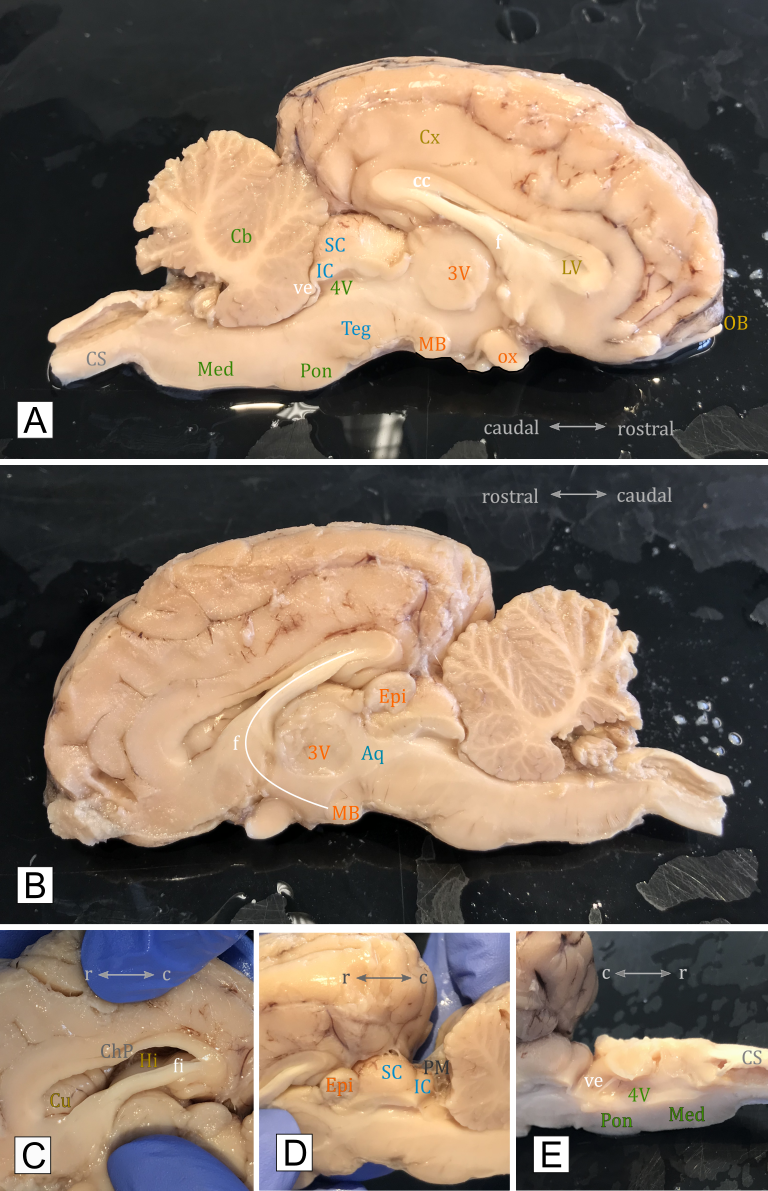
\includegraphics[width=\textwidth]{pictures/Bilder_Jule/Schaf/mittsagittal/schaf_mittsagittal_alle.png}
\end{minipage}
\caption[Midsagittalschnitt Schaf]{\textbf{Midsagittalschnitt Schaf. A}: linke Hemisphäre, \textbf{B}: rechte Hemisphäre, \textbf{C}: lateraler Ventrikel, \textbf{D}: Vierhügelplatte, \textbf{E}: Rhombencephalon ohne Cerebellum. Dabei ist in allen Bildern superior oben und inferior unten dargestellt. Bereiche, die dem Telencephalons zuzuordnen sind, sind gelblich bis bräunlich beschriftet, Bereiche des Diencephalons orange, des Mesencephalons blau und des Rhombencephalons grün. Fasern, bzw. Nerven sind mittels weißer Beschriftung gekennzeichnet. Fasern sind weiß dargestellt.}
\label{fig:schaf_midsagittal}
\end{figure}


\newpage
\subsection{Laterale Sagittalschnitte}
\label{subsec:lateral_sagittal}
%%%%%%%%%%%%%%%%%%%%%%%%%%%%%%%%%%%%%%%%%%%%%%%%%%%%%%%

\begin{figure}[H]
    \centering
    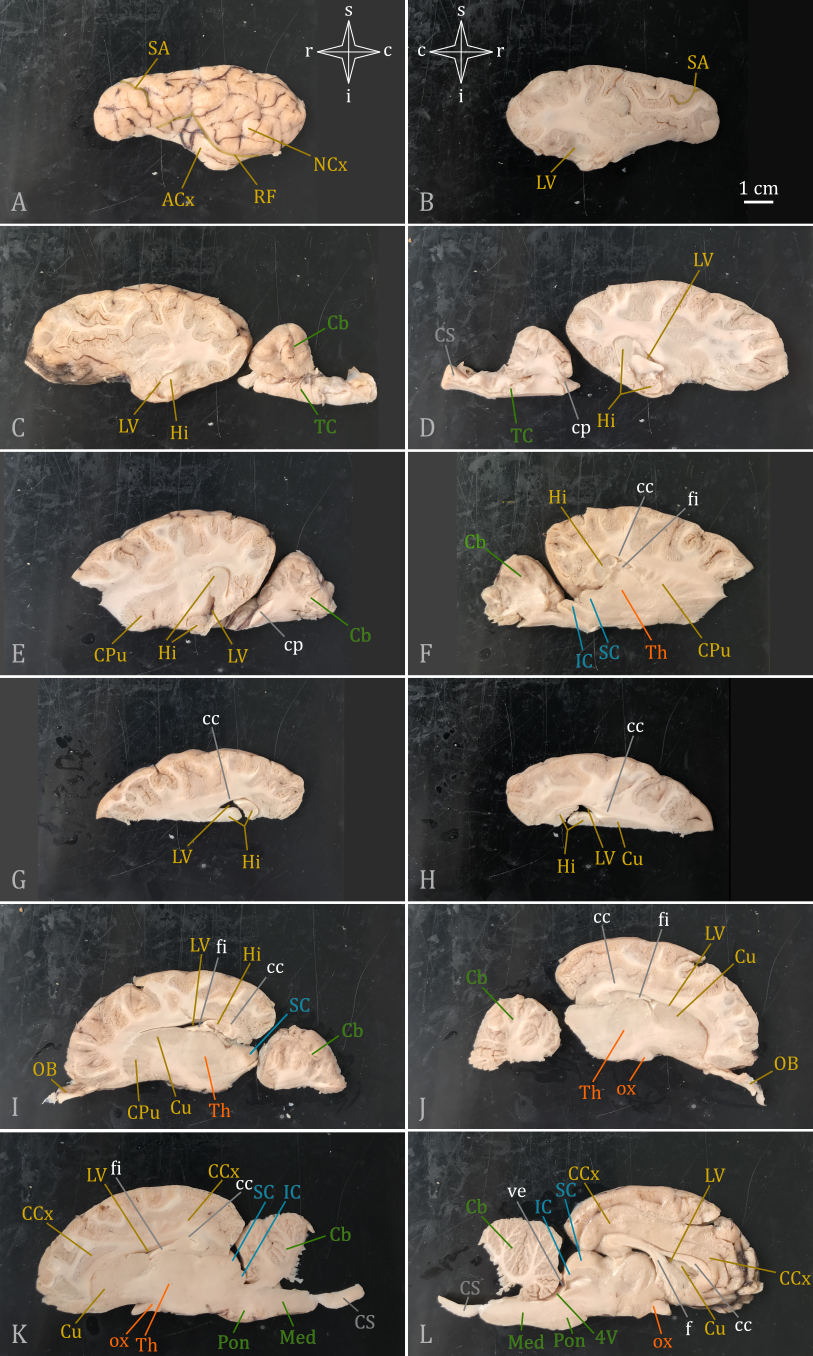
\includegraphics[width=0.8\textwidth]{pictures/Bilder_Jule/Schaf/lateral_sagittal/schaf_lateral_sagittal.png}
    \caption[Laterale Sagittalschnitte Schaf]{\textbf{Laterale Sagittalschnitte Schaf.} Die Schnitte sind von lateral (oben) nach medial (unten) angeordnet. Bereiche des Telencephalons sind gelb gekennzeichnet, Bereiche des Diencephalons orange, des Mesencephalons blau und des Rhombencephalons grün. Fasern sind weiß dargestellt.}
    \label{fig:schaf_lateral_sagittal}
\end{figure}


\newpage
\subsection{Coronalschnitte}
\label{subsec:coronal}
%%%%%%%%%%%%%%%%%%%%%%%%%%%%%%%%%%%%%%%%%%%%%%%%%%%%%%%

\begin{figure}[H]
\centering
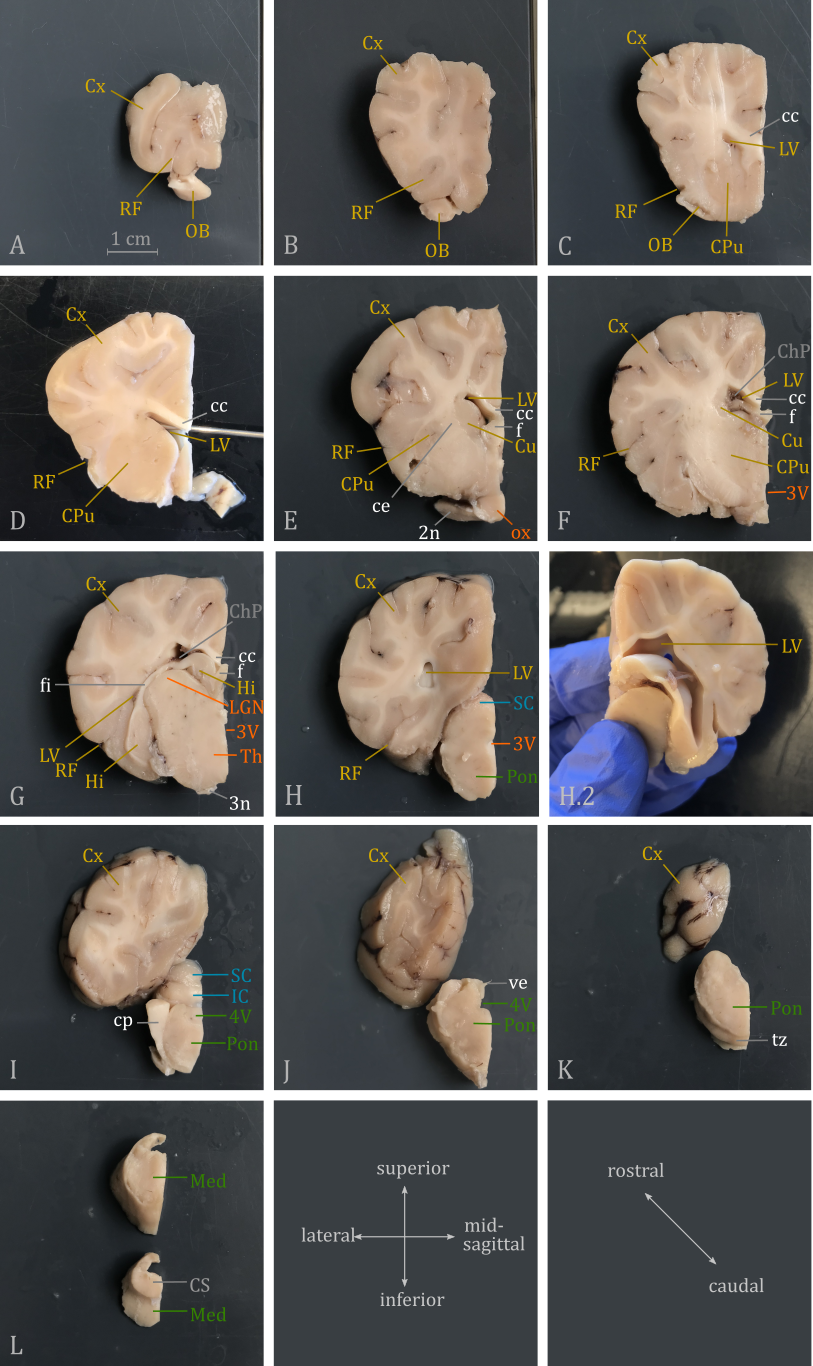
\includegraphics[width=0.8\textwidth]{pictures/Bilder_Jule/Schaf/coronal/coronal_schaf_all.png}
\caption[Coronalschnitte Schaf]{\textbf{Coronalschnitte Schaf.} Von rostral (links oben) nach caudal (rechts unten). Teilgebiete des Telencephalons sind gelb, des Diencephalons orange, des Mesencephalons blau und des Rhombencephalons grün beschriftet. Fasern, bzw. Nerven sind in weiß beschriftet.}
\label{fig:coronal_schaf}
\end{figure}

\subsection{Beschriftung und Kürzel}
%%%%%%%%%%%%%%%%%%%%%%%%%%%%%%%%%%%%%%%%%%%%%%%%%%%%%%%


\begin{table}[H]
\begin{tabular}{llcll}
           & 3V  & - & dritter Ventrikel                                                       & \multicolumn{1}{c}{\textbf{}} \\
\textbf{}  & 3n  & -          & Nervus oculomotorius                                                        & \multicolumn{1}{c}{}          \\
\textbf{}  & 4V  & -          & vierter Ventrikel                                                       & \multicolumn{1}{c}{}          \\
\textbf{A} & ACx & -          & Archicortex                                                             & \multicolumn{1}{c}{}          \\
\textbf{}  & Aq  & -          & Aquädukt, Aqueductus mesencephali, Aquaeductus cerebri                  & \multicolumn{1}{c}{}          \\
\textbf{C} & Cb  & - & Cerebellum, Kleinhirn                                                   & \multicolumn{1}{c}{\textbf{}} \\
           & cc  & - & Corpus callosum                                                         & \multicolumn{1}{c}{\textbf{}} \\
\textbf{}  & CCx & -          & cingulärer Cortex, Gyrus cinguli             & \multicolumn{1}{c}{}          \\
\textbf{}  & ce  & -          & Capsula externa                                                         & \multicolumn{1}{c}{}          \\
\textbf{}  & Chp & -          & Plexus choroideus                                                          & \multicolumn{1}{c}{}          \\
\textbf{}  & cp  & -          & Kleinhirn-Pedunkel                                                      & \multicolumn{1}{c}{}          \\
\textbf{}  & CPu & -          & Caudoputamen                                                            &                               \\
\textbf{}  & CS  & -          & Rückenmark                                                              &                               \\
\textbf{}  & Cu  & -          & Nucleus caudatus                                                        &                               \\
\textbf{}  & Cx  & -          & cerebraler Cortex, Cortex cerebri          &                               \\
\textbf{E} & Epi & -          & Epiphyse                                                                &                               \\
\textbf{F} & f   & -          & Fornix                                                                  &                               \\
\textbf{}  & fi  & -          & Fimbria                                                                 &                               \\
\textbf{H} & Hip & -          & Hippocampus                                                             &                               \\
\textbf{I} & IC  & -          & Colliculus inferior                                                     &                               \\
\textbf{L} & LGN & -          & Corpus geniculatum laterale                                             &                               \\
\textbf{}  & LV  & -          & lateraler Ventrikel                                                     &                               \\
\textbf{M} & MB  & -          & Mammillarkörper                                                         &                               \\
\textbf{}  & Med & -          & Medulla, Medulla oblongata                  &                               \\
\textbf{N} & NCx & -          & Neocortex                                                               &                               \\
\textbf{O} & OB  & -          & Riechkolben, Bulbus olfactorius                                                      &                               \\
\textbf{}  & ox  & -          & optisches Chiasma, Chiasma opticum           &                               \\
\textbf{P} & PM  & -          & Pia mater                                                               &                               \\
\textbf{}  & Pon & -          & Pons                                                                    &                               \\
\textbf{R} & RF  & -          & Fissura rhinalis                                                        &                               \\
\textbf{S} & SA  & -          & Sulcus ansatus                                                          &                               \\
\textbf{}  & SC  & -          & Colliculus superior                                                     &                               \\
\textbf{T} & TC  & -          & Hirnstamm, Truncus cerebri, Truncus encephali &                               \\
\textbf{}  & Teg & -          & Tegmentum, Tegmentum mesencephali           &                               \\
\textbf{}  & Th  & -          & Thalamus                                                                &                               \\
\textbf{}  & tz  & -          & Trapezkörper                                                            &                               \\
\textbf{V} & ve  & -          & Velum                                                                   &                              
\end{tabular}
\end{table}
%%%%%%%%%%%%%%%%%%%%%%%%%%%%%%%%%%%%%%%%%%%%%%%%%%%%%%%%%%%
%%%%%%%%%%%%%%%%%%%%%%%%%%%%%%%%%%%%%%%%%%%%%%%%%%%%%%%%%%%

\newpage
\section{Allgemeine Übersicht}
%%%%%%%%%%%%%%%%%%%%%%%%%%%%%%%%%%%%%%%%%%%%%%%%%%%%%%%%%%%
%%%%%%%%%%%%%%%%%%%%%%%%%%%%%%%%%%%%%%%%%%%%%%%%%%%%%%%%%%%

\subsection{Telencephalon}
\label{subsec:Telencephalon} \index{Telencephalon}
%%%%%%%%%%%%%%%%%%%%%%%%%%%%%%%%%%%%%%%%%%%%%%%%%%%%%%%%%%%
%%%%%%%%%%%%%%%%%%%%%%%%%%%%%%%%%%%%%%%%%%%%%%%%%%%%%%%%%%%

Das Telencephalon oder das Endhirn ist eines der fünf Hirnareale, in die sich das Gehirn nach der Cephalisation gliedern lässt. Das Telencephalon befindet sich am rostralen Ende des Gehirns und überdeckt bei Säugern teilweise das superiore Diencephalon. Auch Bereiche des Mesencephalons können von ihm verdeckt werden. Generell kann das Telencephalon in cortikale Gebiete (Großhirnrinde), Mark (weiße Substanz) und subcortikale Kerngebiete, zu denen die Basalganglia und die Amygdala gehören, unterteilt werden. 

\subsubsection{Großhirnrinde}
\label{subsubsec:Grosshirnrinde}
%%%%%%%%%%%%%%%%%%%%%%%%%%%%%%%%%%%%%%%%%%%%%%%%%%%%%%%%%%%

Der cerebrale Cortex (\textit{Cortex cerebri}) \index{Cortex! cerebri} umhüllt das Gehirn und macht bei Säugern den größten Teil der Außenfläche des Gehirns aus. Er besteht aus zwei Hemisphären, die durch einen dicken Faserstrang, den \textit{Corpus callosum} \index{Corpus! callosum} oder Balken, miteinander in Verbindung stehen. Im Laufe der Evolution expandierte der cerebrale Cortex der Säuger und verdeckt dadurch jene Strukturen des Endhirns, die innerhalb der Hemisphären liegen. Im Allgemeinen dient die Großhirnrinde der Analyse und Integration sensorischer Information, sowie der Verknüpfung  dieses Inputs mit bereits gespeicherten Informationen und Erfahrungen. Des Weiteren ist der cerebrale Cortex die 'Steuerzentrale' von Verhalten, das weit über simple Reflexe und Reaktionen hinausreicht. Diese analytischen und integrativen Fähigkeiten des Cortex resultieren aus seiner zellulären Organisation, sowie aus der Kommunikation mit den restlichen Strukturen des zentralen Nervensystems \textsuperscript{\cite[7]{watson2010thebrain}}.


\subsubsection*{Faltung der Großhirnrinde}
%%%%%%%%%%%%%%%%%%%%%%%%%%%%%%%%%%%%%%%%%%%%%%%%%%%%%%%%%%%

Basierend auf der cortikalen Faltung können Säugetiere in lissencephale und gyrencephale Spezies unterteilt werden. Die Oberfläche des Cerebralcortex der Ratte als \textbf{lissencephale Spezies}\index{lissencephal} ist eben, bzw. glatt strukturiert. Im Gegensatz dazu weist der cerebrale Cortex von \textbf{gyrencephalen Spezies}\index{gyrencephal}, wie dem Schaf oder der meisten Primaten, zahlreiche Furchen (Sulci, Fissurae) und Windungen (Gyri) auf. Die Sulci und vor allem die Fissurae reichen bis in tiefere Ebenen des Cortex und vergrößern somit dessen Gesamtoberfläche \textsuperscript{\cite[7]{watson2010thebrain}}. Anhand dieser Fissurae und Sulci kann der cerebrale Cortex in vier Hirnlappen, \textit{Lobi cerebri}\index{Lobi cerebri}, unterteilt werden. Es kann zwischen Frontallappen, Temporallappen, Parietallappen und Okzipitallappen unterschieden werden (Abb.~\ref{fig:cortex_lappen}).\\

\noindent Die \textbf{Insula}\index{Insula}, auch Inselrinde oder \textit{Gyrus insularis}, befindet sich tief innerhalb des Sulcus lateralis und wird vom Temporal-, Parietal- und Frontallappen überdeckt. Der Bereich des cerebralen Cortex, der sie verdeckt, wird auch \textbf{Operculum} genannt. Die Insula ist an der Regulation von Emotionen und der Homoöstase beteiligt \textsuperscript{\cite[15]{kandel2013principles}}. Des Weiteren prozessieren Neurone der Insula Informationen, die den 'inneren Zustand' des Körpers betreffen und bei autonomen Komponenten der Schmerz-Antwort mitwirken (Kap.~\ref{subsubsec:Schmerzsinn}) \textsuperscript{\cite[24]{kandel2013principles}}. Ebenfalls ein besonderer Gyrus ist der \textbf{cinguläre Cortex}\index{Cortex! cinguli} (\textit{Gyrus cinguli}). Er umgibt die dorsale, bzw. superiore Oberfläche des Corpus callosum (Abb.~\ref{fig:schaf_lateral_sagittal}~K,L) und ist als Teilgebiet des limbischen Systems (Kap.~\ref{subsec:limisches_system}) in die Regulation von Emotionen und Kognition involviert \textsuperscript{\cite[15]{kandel2013principles}}.

\begin{figure}[H]
	\centering
	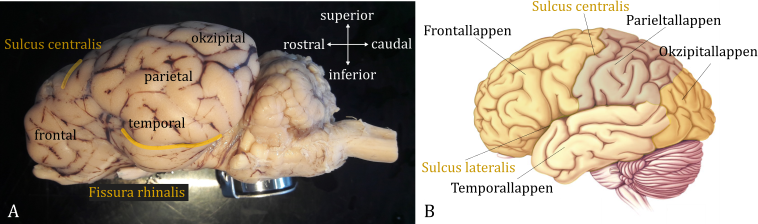
\includegraphics[width=\textwidth]{pictures/Bilder_Jule/Andere/grosshirnrinde.png}
	\caption[Lappen und Sulci der Großhirnrinde]{\textbf{Lappen und Sulci der Großhirnrinde.} \textbf{A:} Großhirnrinde des Schafes, \textbf{B:} Großhirnrinde des Menschen. Die Großhirnrinde (gelb bis bräunlich) kann anhand der Sulci in vier Lappen (\textit{Lobi cerebri}) unterteilt werden: Frontallappen, Parietallappen, Temporallappen und Okzipitallappen\index{Lobi cerebri}. \\
	Abbildung B nach \textit{Neuroanatomy}, Crossman und Neary \textsuperscript{\cite[7]{crossman2014neuroanatomy}}.}
	\label{fig:cortex_lappen} 
\end{figure}

\noindent Die besonders großen und bedeutenden Sulci werden auch Fissuren genannt. Die wohl auffallendste unter ihnen ist die \textbf{Fissura longitudinalis cerebri}\index{Fissura! longitudinalis cerebri}. Sie befindet sich zwischen den beiden Großhirnhemisphären. Unter ihr liegt der Corpus callosum\index{Corpus! callosum}, die einzige Verbindung der beiden Hemisphären. Der \textbf{Sulcus centralis}\index{Sulcus! centralis} erstreckt sich in superior-inferiorer Richtung und trennt den Frontallappen vom Parietallappen. Der \textbf{Sulcus lateralis}\index{Sulcus! lateralis} oder auch \textit{Fissura sylvii} erstreckt sich entlang der rostro-caudalen Achse und trennt den Temporallappen vom Frontal- und Parietallappen (Abb.~\ref{fig:cortex_lappen}~B) \textsuperscript{\cite[7]{neurowissenschaften_baer}}. Ein weiterer, bedeutender Sulcus ist die \textbf{Fissura rhinalis}\index{Fissura! rhinalis} (Abb.~\ref{fig:cortex_lappen}~A), die den Neocortex räumlich vom Archicortex trennt. 

\subsubsection*{Lappen der Großhirnrinde}
%%%%%%%%%%%%%%%%%%%%%%%%%%%%%%%%%%%%%%%%%%%%%%%%%%%%%%%%%%%

Aufgrund der Gyri und Sulci lässt sich die Großhirnrinde in vier verschiedene Lappen, die \textit{Lobi cerebri}\index{Lobi cerebri}, einteilen (Abb.~\ref{fig:cortex_lappen}). Jedem Lobus können dabei verschiedene Funktionen zugeordnet werden. Der rostral gelegene \textbf{Frontallappen} ist am Kurzzeitgedächtnis, der Planung zukünftiger Handlungen, sowie an der Steuerung der Motorik beteiligt. Der laterale \textbf{Temporallappen} kann mit dem Hören assoziiert werden. Zudem ist er durch die tiefer gelegenen Strukturen des Hippocampus und der Amygdala an Lernvorgängen, Gedächtnisbildung und der Entstehung von Emotionen beteiligt. Der \textbf{Parietallappen} ist caudal hinter dem Frontallappen und superior des Temporallappens lokalisiert. In ihm wird die somatosensorische Wahrnehmung prozessiert. Dabei entsteht ein Eindruck des eigenen Körpers relativ zur räumlichen Umgebung. Der vierte Lobus ist der \textbf{Okzipitallappen}, der sich am caudalen Ende der Großhirnrinde befindet. Er enthält die primären und auch höheren visuellen Areale \textsuperscript{\cite[1]{kandel2013principles}}.

\subsubsection*{Sensorische und Motorische Felder}
\label{subsubsec:Sens_Mot_Felder}
%%%%%%%%%%%%%%%%%%%%%%%%%%%%%%%%%%%%%%%%%%%%%%%%%%%%%%%%%%%

\index{Sensorik! allgemein}
In der Großhirnrinde findet die Informationsverarbeitung in verschiedenen Arealen statt. Sie lässt sich funktionell in \textbf{primär motorische}\index{Motorik! allgemein} und \textbf{primär sensorische Felder} unterteilen. Der primäre Motorcortex (M1) enthält Neurone, die an den $\upalpha$-Motorneuronen im Ventralhorn des Rückenmarks enden. Er ist rostral des \textit{Sulcus centralis}\index{Sulcus! centralis}, auf dem \textit{Gyrus praecentralis}\index{Sulcus! praecentralis}, lokalisiert. Zu den primären sensorischen Feldern gehören der primäre visuelle Cortex (V1) am caudalen Ende des Okzipitallappens, der primäre auditorische Cortex (A1) im Temporallappen, sowie der primäre somatosensorische Cortex (S1) caudal des \textit{Sulcus centralis} auf dem \textit{Gyrus postcentralis}. Alle drei primären sensorischen Felder erhalten hauptsächlich unimodale Information aus den zugehörigen thalamischen Kernen. Dabei ist jedes Sinnesorgan, also Augen, Ohren und die Haut, mehrfach im zugehörigen sensorischen Feld repräsentiert. Diese Repräsentation zeigt dabei eine retinotope, tonotope, bzw. somatotope Organisation. Die \textbf{Topologie}, also die Lagebeziehung, der abgebildeten Information bleibt dabei bestehen. Das Größenverhältnis einzelner Teilgebiete wird jedoch nicht zwingend beibehalten \textsuperscript{\cite[14]{penzlin2005tierphys}}. Oft findet eine \textbf{Überrepräsentation} verhaltensrelevanter Bereiche in den primären sensorischen oder motorischen Cortices statt. Beispielsweise werden bei Säugern der retinale Bereich der Fovea im V1 \textsuperscript{\cite{overrepresentation_fovea}}, sowie einige Bereiche der Körperoberfläche in S1 und M1 \textsuperscript{\cite[14]{penzlin2005tierphys}}, überrepräsentiert. Die \textbf{sekundären}, \textbf{tertiären}, usw. \textbf{Repräsentationsfelder} sind den primären untergeordnet. Die sekundären Felder erhalten spezifische thalamische Projektionen.\\

\begin{figure}[H]
    \centering
    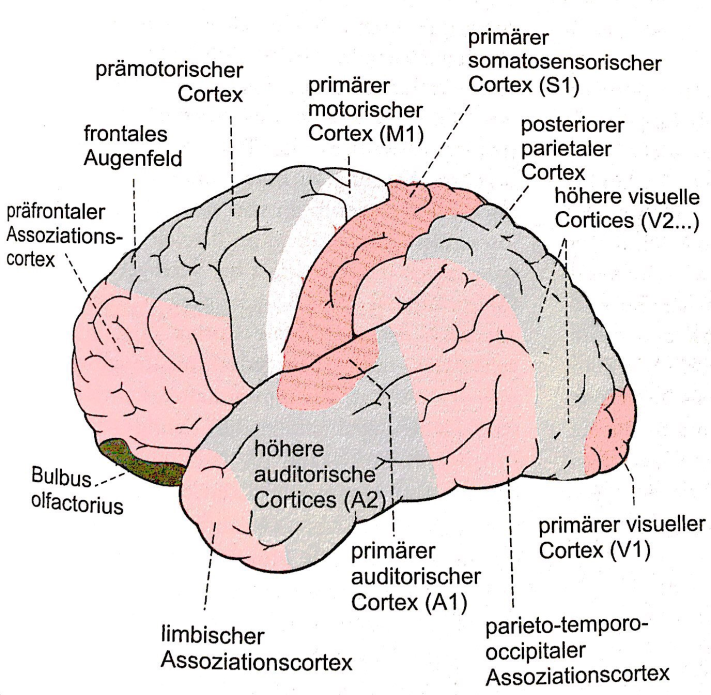
\includegraphics[width=0.69\textwidth]{pictures/Bilder_Jule/Andere/Grosshirnrinde_sensorik_motorik.png}
    \caption[Sensorische, motorische und assoziative Areale der Großhirnrinde]{\textbf{Sensorische, motorische und assoziative Areale der Großhirnrinde.} Abbildung aus \textit{Lehrbuch der Tierphysiologie}, Pezlin \textsuperscript{\cite[14]{penzlin2005tierphys}}.}
    \label{fig:grosshirnrinde_sensorik_motorik}
\end{figure}

\noindent Jene Felder, die weder den sensorischen noch den motorischen Feldern zugeordnet werden können, werden als sogenannter unspezifischer oder \textbf{assoziativer Cortex} bezeichnet. In diesen Arealen findet eine Verknüpfung oder Integration von motorischer und multisensorischer Information statt \textsuperscript{\cite[14]{penzlin2005tierphys}}. 

\noindent Die Ausdehnung der Projektionsfelder, sowie das Verhältnis zwischen den motorischen und sensorischen Feldern und den Assoziationsfeldern variiert zwischen den verschiedenen Tierklassen: Zum einen nimmt der Anteil der assoziativen, unspezifischen Felder mit der Höherentwicklung zu \textsuperscript{\cite[14]{penzlin2005tierphys}}. Zum anderen sind Felder, die für die Lebensweise einer Tierart besonders relevant sind, wie zum Beispiel das olfaktorische Feld bei Ratten, vergrößert (Abb.~\ref{fig:grosshinrinde_vgl}).

\begin{figure}[H]
    \centering
    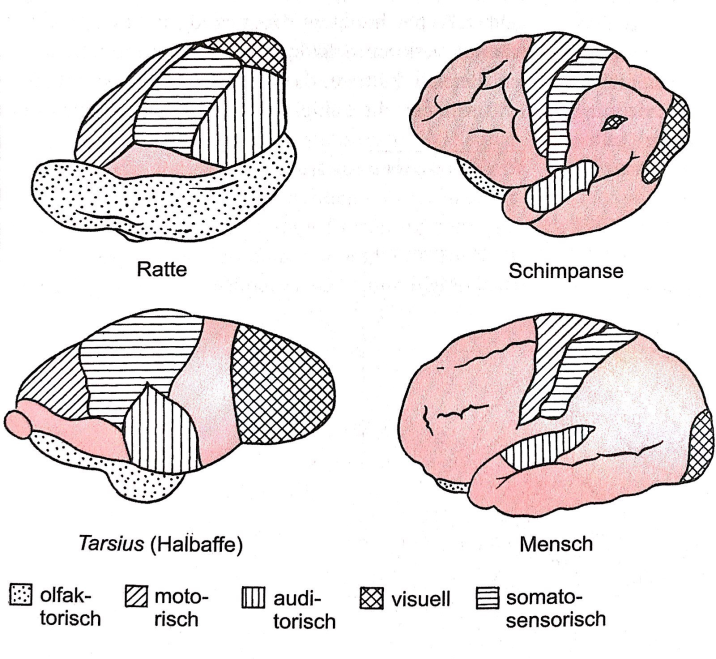
\includegraphics[width=0.7\textwidth]{pictures/Bilder_Jule/Andere/grosshirnrinde_vgl.png}
    \caption[Verhältnis sensorischer, motorischer und assoziativer Areale der Großhirnrinde]{\textbf{Verhältnis sensorischer, motorischer und assoziativer Areale der Großhirnrinde.} Dargestellt ist die Ausdehnung der sensorischen und motorischen Projektionsfelder (schwarz-weiß) und der assoziativen Felder (rot) verschiedener Säugetiere. Abbildung aus \textit{Lehrbuch der Tierphysiologie}, Penzlin \textsuperscript{\cite[14]{penzlin2005tierphys}}.}
    \label{fig:grosshinrinde_vgl}
\end{figure}{}

\subsubsection*{Der Neocortex} \index {Neocortex}
%%%%%%%%%%%%%%%%%%%%%%%%%%%%%%%%%%%%%%%%%%%%%%%%%%%%%%%%%%%

Obwohl sich die verschiedenen Areale der Großhirnrinde funktionell unterscheiden und beispielsweise Informationen unterschiedlicher sensorischer Systeme verarbeiten, variiert die Zellschichtung dieser Areale kaum. In evolutionär älteren Arealen des Cortex, wie dem olfaktorischen Cortex, besteht die Großhirnrinde aus nur drei Schichten, während der evolutionär jüngere \textbf{Neocortex}, auch Isocortex, aus sechs Schichten aufgebaut ist. Diese zellulären Schichten bilden die sogenannte \textbf{graue Substanz}\index{graue Substanz} des (Neo-)Cortex, die viele Zellkörper, jedoch wenige Fasern enthält. Diese Schichten werden von Außen nach Innen nummeriert und bestehen aus drei prominenten Zelltypen: exzitatorische Pyramidenzellen, Körnerzellen, zu denen auch die bedornten Sternzellen (\textit{spiny stellate cells}) gehören, und inhibitorische Interneurone. Jede der sechs Zellschichten des Neocortex besitzt charakteristische Zellen und  Verknüpfungen (Abb.~\ref{fig:neoccortex_schichtung}) \textsuperscript{\cite[7]{watson2010thebrain}}. 

\begin{figure}[H]
	\centering
	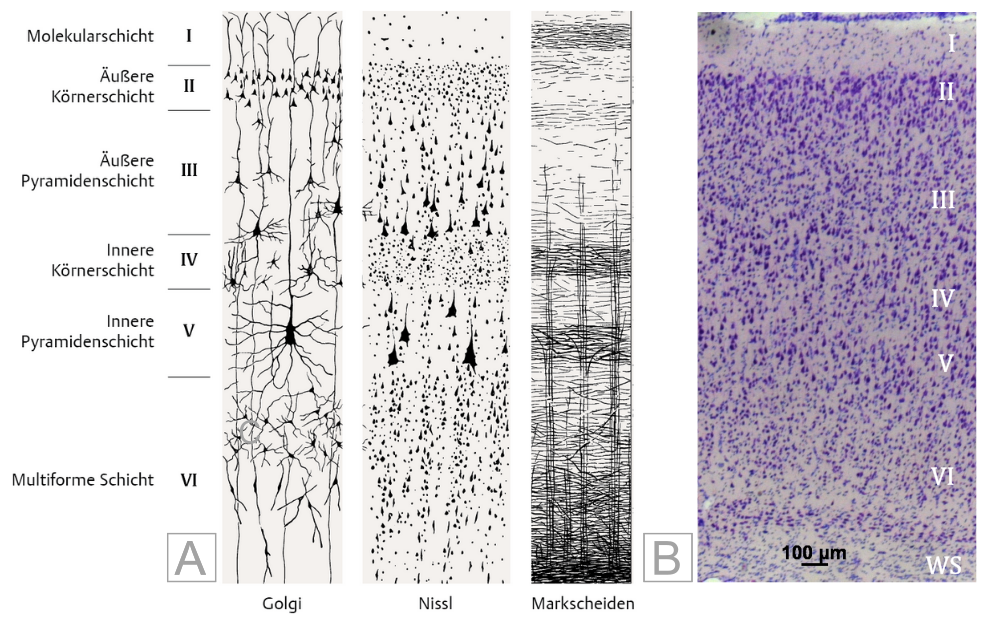
\includegraphics[width=\textwidth]{pictures/Bilder_Jule/Andere/neocortex_schichtung.png}
	\caption[Schichtung des Neocortex]{\textbf{Schichtung des Neocortex.} \textbf{A}:~Schematische Darstellung der Schichten des Neocortex des Menschen unter Verwendung der Golgi-, Nissl- und Markscheidenfärbung. \textbf{B}:~Mikroskopie des Neocortex der Ratte unter Verwendung der Nisslfärbung. WS = weiße Substanz - darüber die sechsschichtige graue Substanz.\\
	Abbildung A aus \textit{Taschenlehrbuch Histologie}, Lüllmann-Rauch und Asan \textsuperscript{\cite{taschenbuch_histologie}}.}
	\label{fig:neoccortex_schichtung}
\end{figure}

\noindent Die \textbf{Molekularschicht} stellt die äußerste Schicht dar. Diese dünne Faserschicht beinhaltet nur wenige Zellkörper, jedoch viele dendritische Fortsätze und stellt somit eine Verarbeitungsstruktur des Cortex dar. Unter ihr liegt die \textbf{äußere Körnerschicht}. Sie besteht aus zahlreichen kleinen Pyramidenzellen, sowie kleinen inhibitorischen Zellen. Diese agieren in kleinen neuronalen Schaltkreisen um einkommende Information zu prozessieren. Die dritte Zellschicht, die \textbf{äußere Pyramidenschicht}, zeichnet sich durch eine Vielzahl größerer Pyramidenzellen aus. Diese senden exzitatorische Signale in benachbarte oder auch weit entfernte Areale des Cortex. Korbzellen (\textit{basket cells})  und andere inhibitorische Zellen inhibieren benachbarte Zellen und ermöglichen somit weitere cortikale Informationsverarbeitung. In der vierten Schicht, der \textbf{inneren Körnerschicht}, enden viele thalamische Fasern. Sie besteht aus zahlreichen kleinen Sternzellen. Unter ihr liegt die \textbf{innere Pyramidenschicht}, die aus den größten Pyramidenzellen des Neocortex aufgebaut ist. Ihre Axone, die bis weit außerhalb des Neocortex reichen, terminieren unter anderem im Striatum und Spinalkanal. Die am tiefsten gelegene Schicht ist die sechste, \textbf{multiforme Schicht}. Diese Schicht ist aus vielen kleinen Zellen aufgebaut, unter anderem aus kleinen Pyramidenzellen, die in den Thalamus projizieren. Diese Verbindungen schließen die Rückkopplungsschleife zwischen Cortex und Thalamus, die die thalamische Aktivität reguliert \textsuperscript{\cite[7]{watson2010thebrain}}.\\
Die neuronalen Netzwerke, die die cortikale Informationsverarbeitung dominieren, zeigen Aktivität, die \textbf{in Säulen organisiert} ist: Die Zellen des Neocortex zeigen die meisten Verbindungen zu Zellen oberhalb und unterhalb der eigenen Position. Dabei weisen einige Zellen inhibitorische Verbindungen zu benachbarten Säulen auf. Diese Verschaltungen scheinen die cortikale Aktivität zu fokussieren.\\
\noindent Unterhalb der neocortikalen Schichten liegt die sog. \textbf{weiße Substanz}\index{weiße Substanz} - eine dichte Schicht aus axonalen Fasern, die nur wenige Zellkörper beinhaltet. Diese Fasern ermöglichen die Verbindung und Kommunikation verschiedener Areale des Cortex, sowie die Kommunikation mit dem Rest des Nervensystems \textsuperscript{\cite[7]{watson2010thebrain}}.

\subsubsection*{Der Allocortex} \index{Allocortex}
%%%%%%%%%%%%%%%%%%%%%%%%%%%%%%%%%%%%%%%%%%%%%%%%%%%%%%%%%%%

Der sogenannte Allocortex setzt sich aus dem Archicortex und dem Paleocortex zusammen und ist, genau wie der Neocortex, Teil der Großhirnrinde. Der mediale \textbf{Archicortex}\index{Archicortex} der Säugetiere ist aus drei Zellschichten aufgebaut und wird auch Hippocampusregion genannt. Die \textbf{Fissura rhinalis} trennt den evolutionär älteren Archicortex vom jüngeren, sechsschichtigen Neocortex (Abb.~\ref{fig:allocortex_ratte}) \textsuperscript{\cite[6]{storch2012lehrbuchzoo}}. Neben dem Hippocampus ist auch der cinguläre Cortex\index{Cortex! cinguli} (Kap.~\ref{subsubsec:Grosshirnrinde}, Kap.~\ref{subsec:limisches_system}) ein Teilgebiet des Archicortex. Der lateral gelegene \textbf{Paleocortex}\index{Paleocortex} ist das älteste Teilgebiet der Großhirnrinde. Genau wie der Archicortex besteht er aus drei Zellschichten \textsuperscript{\cite[6]{storch2012lehrbuchzoo}}. Er bildet bei Säugern das Riechhirn und beinhaltet den primären olfaktorischen Cortex, den Bulbus olfactorius\index{Bulbus olfactorius}, sowie die cortikalen Bereiche der Amygdala\index{Amygdala} \textsuperscript{\cite[9]{trepel2011neuroanatomie}}.

\begin{figure}[H]
    \centering
    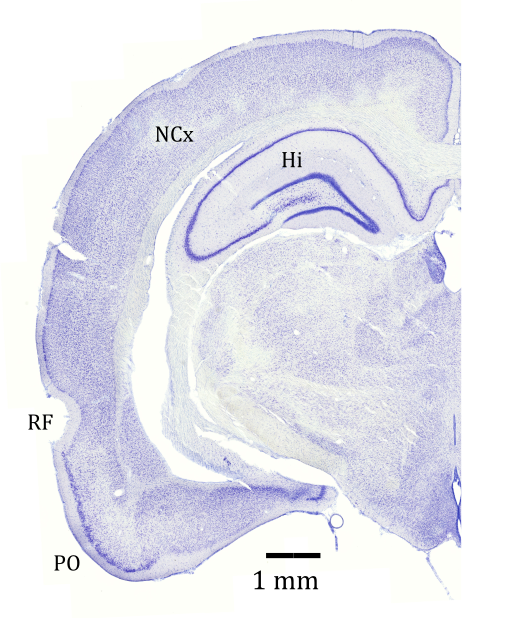
\includegraphics[width=0.38\textwidth]{pictures/Bilder_Jule/Ratte/RF.png}
    \caption[Großhirnrinde Ratte]{\textbf{Großhirnrinde Ratte.} Coronaler Querschnitt durch eine Hemisphäre des Rattengehirns (N21-3). Der dreischichtige Hippocampus (Hi) ist Teil des Archicortex, der dreischichtige primäre olfaktorische Cortex (PO) gehört zum Paleocortex. Die Fissura rhinalis (RF) trennt den sechsschichtigen Neocortex (NCx) vom Paleocortex.}
    \label{fig:allocortex_ratte}
\end{figure}{}

\subsubsection*{Hippocampus}
\label{subsubsec:Hippocampus} \index{Hippocampus}
%%%%%%%%%%%%%%%%%%%%%%%%%%%%%%%%%%%%%%%%%%%%%%%%%%%%%%%%%%%

Das Wort 'Hippocampus' kommt aus dem Griechischen und bedeutet Seepferdchen. Der Hippocampus ist Teil des Archicortex und folglich aus drei Zellschichten aufgebaut. Sowohl bei Menschen, als auch bei der Ratte zeichnet sich der Hippocampus durch eine c-förmige Struktur aus \textsuperscript{\cite[20]{paxinos2014rat}}, die den Thalamus umgibt (Abb.~\ref{fig:hippocampus_schaf}). Er hängt dabei am inneren Rand der Großhirnrinde und liegt zum Großteil an den medialen Wänden der lateralen Ventrikel. Caudal reicht der Hippocampus bis vor zur Vierhügelplatte. Superior reicht er bis an den \textit{Corpus callosum}, wo er unterhalb des Balkens in die Faserstruktur des \textbf{Fornix}\index{Fornix} übergeht, der bis in den \textbf{Mammillarkörper} zieht. Die \textbf{Fimbria}\index{Fimbria} enthält afferente und efferente Fasern und geht in den Fornix über \textsuperscript{\cite[9]{trepel2011neuroanatomie}}.\\

\begin{figure}[H]
    \centering
    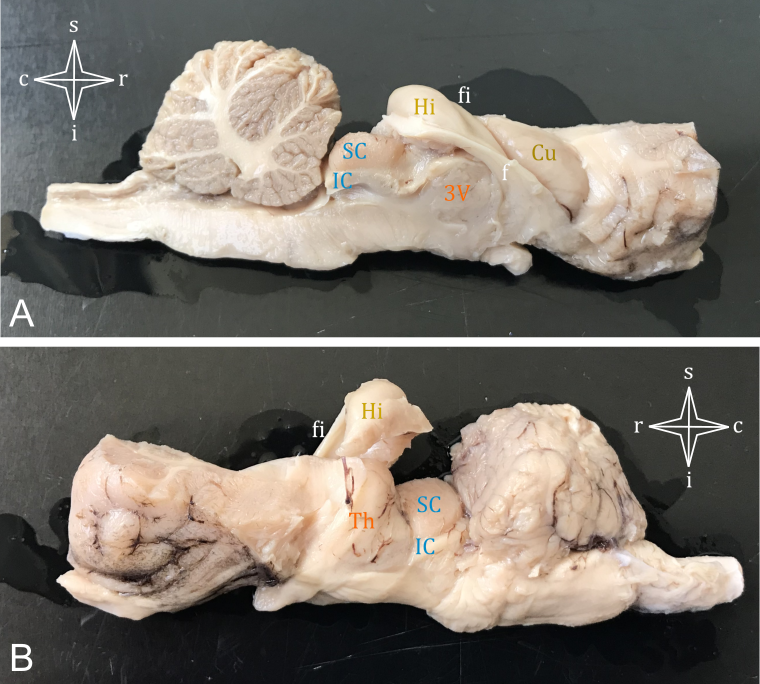
\includegraphics[width=0.6\textwidth]{pictures/Bilder_Jule/Schaf/Ausschnitte/hippocampus_schaf.png}
    \caption[Hippocampus Schaf]{\textbf{Hippocampus Schaf.} Gezeigt ist das Ergebnis einer Hippocampus-Präparation am Schafshirn. Dabei wurden die Bereiche der Großhirnrinde, die den Hippocampus verdecken entfernt. Zu sehen sind der Hippocampus (Hi), der den Thalamus (Th) umschließt. Er liegt caudal des Nucleus caudatus (Cu) und rostral der Vierhügelplatte, die aus dem Colliculus superior (SC) und dem Colliculus inferior (IC) besteht. Ebenfalls gekennzeichnet sind die Fimbria (fi), die in den Fornix (f) übergeht, sowie der dritte Ventrikel (3V), dessen Wände in Teilen vom Thalamus gebildet werden.}
    \label{fig:hippocampus_schaf}
\end{figure}{}

\noindent Die afferenten Fasern, die den Hippocampus erreichen, stammen unter anderem aus dem Neocortex und den olfaktorischen Arealen der Großhirnrinde. Über den Fornix erhält er zusätzlich Informationen aus dem Thalamus, dem cingulären Cortex (\textit{Corpus cinguli}) und der Amygdala. Im Fornix\index{Fornix} verlaufen zudem nahezu alle Efferenzen des Hippocampus. Diese enden unter anderem im Septum, in der Amygdala, sowie im Hypothalamus. Der Großteil der Fasern endet jedoch im Mammillarkörper \textsuperscript{\cite[9]{trepel2011neuroanatomie}}.\\

\noindent Als wichtiger Bestandteil des limbischen Systems (Kap.~\ref{subsec:limisches_system}) ist der Hippocampus an emotionalen, endokrinen und vegetativen Vorgängen beteiligt \textsuperscript{\cite[9]{trepel2011neuroanatomie}}. Des Weiteren spielt er eine wichtige Rolle in der Gedächtnisbildung. So ist der Hippocampus beispielsweise für den Transfer von gespeicherter Information vom Kurzzeit- ins Langzeitgedächtnis unabdingbar \textsuperscript{\cite[6]{storch2012lehrbuchzoo}}. Durch synaptische Langzeit-Plastizität wird Information zeitweise im Hippocampus gespeichert. Schließlich werden die Informationen in den Neocortex, den Ort des Langzeitgedächtnisses, transferiert \textsuperscript{\cite[18]{kandel2013principles}}.

\begin{figure}[H]
    \centering
    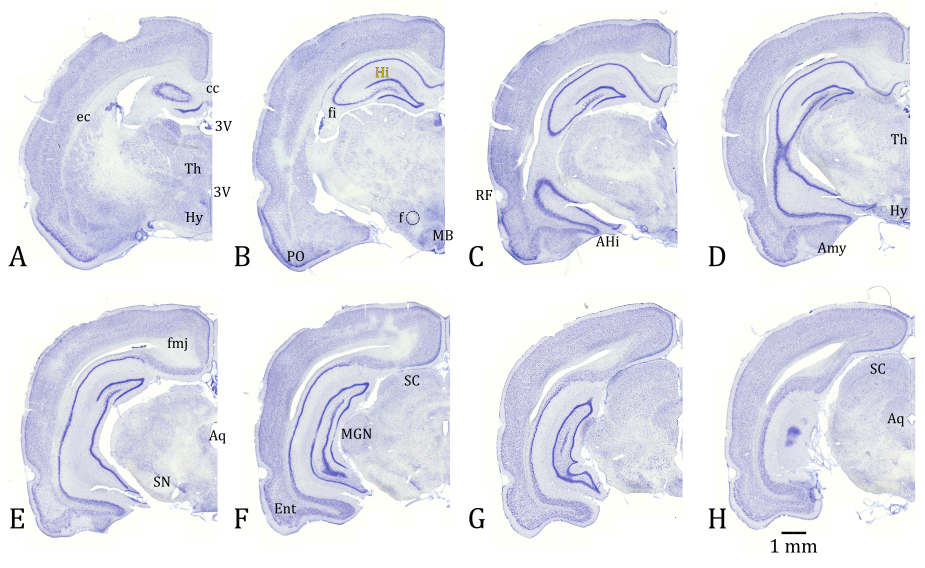
\includegraphics[width=\textwidth]{pictures/Bilder_Jule/Ratte/hippocampus.png}
    \caption[Hippocampus Ratte]{\textbf{Hippocampus Ratte.} Coronalschnitte von rostral nach caudal (A-H: N25-1, N22-2, N20-4, N20-1, N19-1, N18-1, N17-1, N16-1). Gekennzeichnet sind der Hippocampus (Hi), der den Thalamus (Th) umgibt, sowie die Fimbria (fi) und der Fornix (f). Ebenfalls gekennzeichnete Strukturen des Telencephalons: Capsula externa (ec), Corpus callosum (cc), Forceps minor des cc (fmj), Fissura rhinalis (RF), entorhinaler Cortex  (Ent), primärer olfaktorischer Cortex (PO), amygdalo-hippocampisches Areal (AHi), Amygdala (Amy). Strukturen des Diencephalons: dritter Ventrikel (3V), Hypothalamus (Hy), Mammillarkörper (MB), Corpus geniculatum mediale (MGN). Strukturen des Mesencephalons: Aquädukt (Aq), Colliculus superior (SC), Substantia nigra (SN).}
    \label{fig:hippocampus_ratte}
\end{figure}{}

\subsubsection*{Cortico-cortikale Verbindungen}
\label{subsubsec:cortico-cortical}
%%%%%%%%%%%%%%%%%%%%%%%%%%%%%%%%%%%%%%%%%%%%%%%%%%%%%%%%%

Die weiße Substanz, die unter der Oberfläche des Cortex liegt, kann nach ihrem Ursprung, bzw. ihrer Termination, in drei verschiedene Klassen unterteilt werden: Assoziationsfasern, Kommissuren und Projektionsfasern.
\textbf{Assoziationsfasern} verbinden cortikale Areale, die innerhalb derselben Großhirnhemisphäre liegen. Dabei kann zwischen langen und kurzen Fasern unterschieden werden. Durch die kurzen Assoziationsfasern stehen benachbarte cortikale Sulci miteinander in Verbindung. Die langen Fasern ermöglichen eine Interaktion weit entfernter Areale. So sind über die langen Assoziationsfasern die primären sensorischen Areale mit den Assoziationsarealen des Cortex verbunden. Der \textit{Fasciculus longitudinalis inferior}\index{Fasciculus! longitudinalis} (Abb.~\ref{fig:cortico-cortical}) beispielsweise verbindet den Frontal- mit dem Okzipitallappen. Eine seiner Teilgebiete, der \textit{Fasciculus arcuatus}\index{Fasciculus! arcuatus}, vernetzt Gyri des Frontal- und Temporallappens und ist essentiell für die Sprachfunktion. Der \textit{Fasciculus longitudinalis superior}\index{Fasciculus! longitudinalis} verläuft ausgehend vom Okzipitallappen bis hin zum Pol des Temporallappens und trägt so zur visuellen Wiedererkennung bei. Der \textit{Fasciculus uncinatus}\index{Fasciculus! uncinatus} verbindet anteriore und inferiore Bereiche des Frontallappens mit dem Temporallappen. Diese Projektion spielt eine wichtige Rolle in der Regulation von Verhalten. Das \textit{Cingulum}\index{Cingulum} ist im cingulären Cortex (Kap.~\ref{subsubsec:Grosshirnrinde}) lokalisiert. Durch das Cingulum stehen Frontal- und Parietallappen mit dem Gyrus parahippocampalis und angrenzenden temporalen Gyri in Verbindung.

\begin{figure}[H]
    \centering
    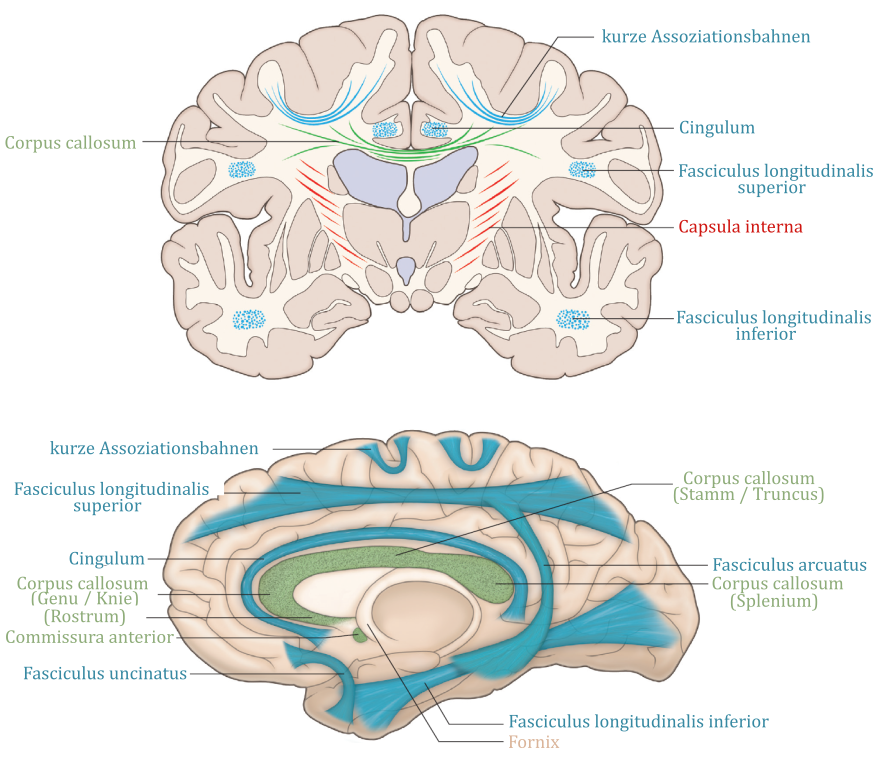
\includegraphics[width=\textwidth]{pictures/Bilder_Jule/Andere/cortico-cortical_(crossm13).png}
    \caption[Cortico-cortikale Verbindungen]{\textbf{Cortico-cortikale Verbindungen.} Verlauf der neuronalen Bahnen des cerebralen Cortex in der Coronal-Ebene (oben) und Midsagittal-Ebene (unten).\\
    Abbildung nach \textit{Neuroanatomy}, Crossman und Neary \textsuperscript{\cite[13]{crossman2014neuroanatomy}}.}
    \label{fig:cortico-cortical}
\end{figure}{}

\noindent \textbf{Kommissuren} (Abb.~\ref{fig:faser_cortico-cortical}) verlaufen von einer Großhirnhemisphäre in die jeweils andere und verbinden somit funktionell verwandte Strukturen. Die wohl auffälligste Kommissur ist der \textit{Corpus callosum}\index{Corpus! callosum}, der zwischen den beiden Großhirnhemisphären verläuft. Er verbindet Bereiche des Neocortex, mit Ausnahme der temporalen Bereiche. Auch das \textit{Splenium} des Corpus callosum gehört zu den Kommissuren. Es verbindet die Okzipitallappen miteinander und trägt so zu visuellen Funktionen bei. Die inferioren und medialen Gyri des Temporallappens, sowie die olfaktorischen Gebiete der beiden Hemisphären, sind über die \textit{Commissura anterior} vernetzt. Den letzten Typ stellen die sogenannten \textbf{Projektionsfasern} dar. Über diese kommuniziert der cerebrale Cortex mit subcortikalen Strukturen, sowie dem Thalamus, dem Striatum, dem Hirnstamm und dem Rückenmark. Die \textit{Capsula interna}\index{Capsula interna} liegt  medial zwischen Thalamus und Nucleus caudatus. Sie kann in verschiedene Teilgebiete differenziert werden und verbindet unter anderem Thalamus und Präfrontallappen, sowie den Thalamus mit dem primären somatosensorischen, auditorischen und visuellen Cortex \textsuperscript{\cite[13]{crossman2014neuroanatomy}}.

\begin{figure}[H]
    \centering
    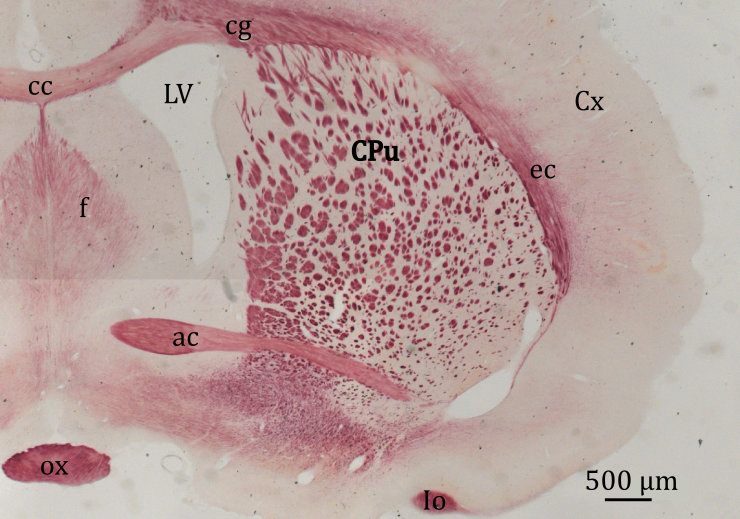
\includegraphics[width=0.45\textwidth]{pictures/Bilder_Jule/Ratte/faser_cortex.png}
    \caption[Kommissuren der Großhirnrinde]{\textbf{Kommissuren der Großhirnrinde.} Coronalschnitt durch das Rattengehirn auf Höhe des Diencephalons (F27-4). Die Commissura anterior (ac), sowie der Corpus callosum (cc) und das Cingulum (cg) sind gekennzeichnet. Ebenfalls sichtbar sind das Chiasma opticum (ox) des Diencephalons und der Fornix (f). Auch der laterale Ventrikel des Telencephalons (LV), der cerebrale Cortex (Cx), das Caudoputamen (CPu), die Capsula externa (ec) und der laterale olfaktorische Trakt (lo) sind zu sehen.}
    \label{fig:faser_cortico-cortical}
\end{figure}

\subsubsection{Amygdala}
\label{subsubsec:Amygdala} \index{Amygdala}
%%%%%%%%%%%%%%%%%%%%%%%%%%%%%%%%%%%%%%%%%%%%%%%%%%%%%%%%%%%

Die Amygdala (\textit{Corpus amygdaloideum}), auch Mandelkern genannt, liegt unterhalb des olfaktorischen Cortex und rostral des Hippocampus (Abb.~\ref{fig:amygdala_ratte}). Sie ist ein subcortikales Gebiet, das in Teilen dem Paleocortex zuzuordnen ist \textsuperscript{\cite[9]{trepel2011neuroanatomie}}. Die Amygdala ist, wie auch der Hippocampus, ein wichtiger Bestandteil des limbischen Systems (Kap.~\ref{subsec:limisches_system}) \textsuperscript{\cite[15]{kandel2013principles}}.

\begin{figure}[H]
    \centering
    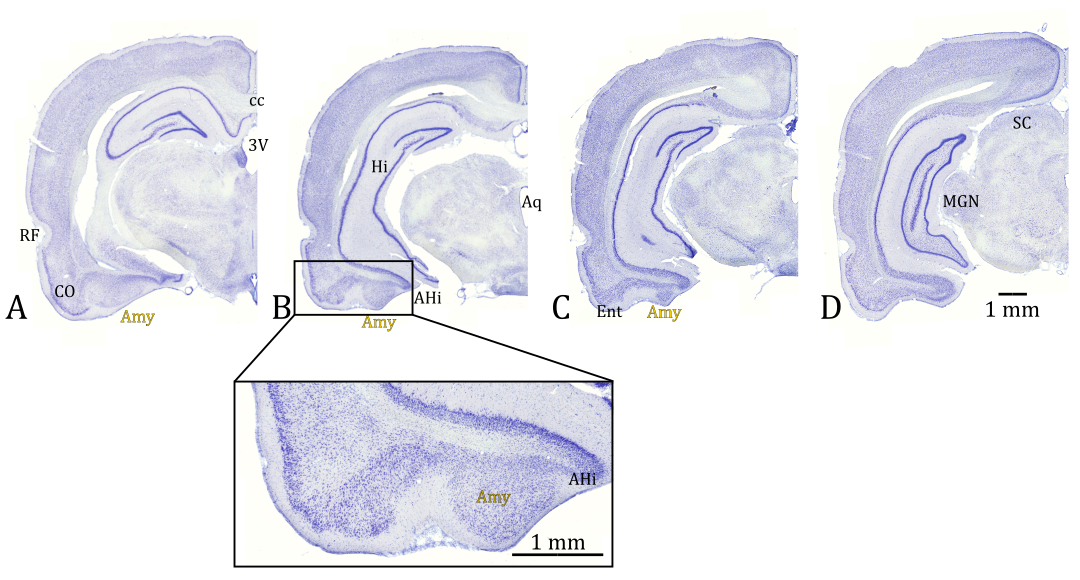
\includegraphics[width=\textwidth]{pictures/Bilder_Jule/Ratte/amygdala.png}
    \caption[Amygdala Ratte]{\textbf{Amygdala Ratte.} Coronalschnitte von rostral nach caudal (A-D: N20-2, N19-3, N18-4, N17-3). Die Amygdala (Amy) liegt unter dem olfaktorischen Cortex (CO). Das amygdalo-hippocampische Areal (AHi) stellt den Übergang zwischen der Amygdala und dem Hippocampus (Hi) dar. Ebenfalls gekennzeichnet sind der Corpus callosum (cc) und die Fissura rhinalis (RF) des Telencephalons, der Corpus geniculatum mediale (MGN) und der dritte Ventrikel (3V) des Diencephalons, sowie das Aquädukt (Aq) und der Colliculus superior (SC) des Mesencephalons.}
    \label{fig:amygdala_ratte}
\end{figure}{}

\noindent Die Amygdala besteht aus mehreren Kernen, die sich in drei Unterbereiche gliedern lassen: Der Zentralbereich steuert vegetative und affektive Grundfunktionen. Der cortico-mediale Bereich verarbeitet olfaktorische Informationen, wie zum Beispiel soziale Gerüche (Pheromone). Der dritte, baso-laterale Teilbereich ist mit Emotionen assoziiert \textsuperscript{\cite[6]{storch2012lehrbuchzoo}}. Im Allgemeinen ist die Amygdala in die Entstehung und Verarbeitung emotionaler Zustände, wie der Angst- und   Vermeidungsreaktion, involviert. Sie spielt auch bei positiven Emotionen, besonders wenn das Belohnungssystem involviert ist, eine Rolle \textsuperscript{\cite[48]{kandel2013principles}}.\\
Die Amygdala erhält direkten und indirekten thalamischen Input. Somit ist sie in der Lage die emotionale Ladung eines Stimulus zu evaluieren. Detektiert sie Gefahr, kann sie, durch ihre starke  Verbindung zu Hypothalamus und Hirnstamm, die Entstehung von physiologischen und endokrinen Antworten und Verhaltensreaktionen dirigieren \textsuperscript{\cite[48]{kandel2013principles}}. Zum Beispiel kann die Amygdala unbewusste Reaktionen auf Angstzustände, wie die Veränderung von Puls, Respirationsrate und Pupillen-Erweiterung,  hervorrufen \textsuperscript{\cite[15]{kandel2013principles}}.
Auch instinktive Prozesse, wie Hunger oder Durst, sowie Prozesse, die Angst-, Aggressions- oder Paarungsverhalten untergeordnet sind, werden von der Amygdala gesteuert \textsuperscript{\cite[18]{kandel2013principles}}.
Die vielseitigen Projektionen, die von der Amygdala ausgehen, erlauben ihr auch andere, kognitive Funktionen zu beeinflussen. Beispielsweise können durch die Amygdala, mittels umfassender Projektionen in cortikale Gebiete, sowohl Aufmerksamkeit, als auch Wahrnehmung, Gedächtnis und Entscheidungsfindung moduliert und somit beeinflusst werden. Durch ihre Verbindung mit den modulatorischen Nuclei, wie Teilen der dopaminergen, noradrenergen und serotonergen Systeme (Kap.~\ref{sec:transmittersysteme}), ist sie zudem in der Lage die kognitive Sachverarbeitung zu beeinflussen \textsuperscript{\cite[48]{kandel2013principles}}.


\subsection{Diencephalon}
\label{subsec:Diencephalon} \index{Diencephalon}
%%%%%%%%%%%%%%%%%%%%%%%%%%%%%%%%%%%%%%%%%%%%%%%%%%%%%%%%%%%
%%%%%%%%%%%%%%%%%%%%%%%%%%%%%%%%%%%%%%%%%%%%%%%%%%%%%%%%%%%

Das Diencephalon oder Zwischenhirn befindet sich caudal, bzw. unterhalb des Telencephalons und umschließt den dritten Ventrikel. Es kann in vier Hauptbereiche gegliedert werden. Von superior nach inferior, bzw. dorsal nach rostral, kann zischen \textbf{Epithalamus}, \textbf{Thalamus}, \textbf{Subthalamus}  und \textbf{Hypothalamus} unterschieden werden \textsuperscript{\cite[16]{crossman2014neuroanatomy}}.

\subsubsection{Epithalamus}
\label{subsubsec:Epithalamus} \index{Epithalamus}
%%%%%%%%%%%%%%%%%%%%%%%%%%%%%%%%%%%%%%%%%%%%%%%%%%%%%%%%%%%

Der Epithalamus ist ein kleines Teilgebiet des Diencephalons. Er ist dorsal und caudal gelegen. Bekannte Komponenten des Epithalamus stellen die Epiphyse (Abb.~\ref{fig:schaf_midsagittal}~B,D) und die Nuclei habenulares\index{Nuclei! habenulares} (Abb.\ref{fig:Diencephalon_Ratte}~B-D) dar, die mit dem limbischen System in Verbindung stehen \textsuperscript{\cite[12]{crossman2014neuroanatomy}}.\\

\noindent Die \textbf{Epiphyse}\index{Epiphyse} (\textit{Epiphysis cerebri}), auch das \textbf{Pinealorgan} (\textit{Glandula pinealis}) oder die \textbf{Zirbeldrüse}, befindet sich mittig im Diencephalon, direkt rostral des Colliculus superior des Mesencephalons. Bei der Epiphyse handelt es sich um ein unpaares endokrines Organ.
Sie besteht aus Gliazellen und Drüsenzellen, den sogenannten Pinealocyten. Letztere stammen von Photorezeptoren ab und synthetisieren das Hormon Melatonin. Die Epiphyse zeigt, unter anderem  bei bei einigen Fischen, noch netzhautartige Strukturen auf. Bei Säugern ist jedoch keine Photosensibilität mehr vorhanden. Zudem verliert die Epiphyse bei Säugern nach der Geburt ihre neuronale Verbindung zum Gehirn. Durch die Ausschüttung von Melatonin ist sie in die Regulierung des Schlaf-Wach-Rhythmus involviert und somit an der Steuerung des circadianen Rhythmus beteiligt. Auch bei der Regulation des Einsetzens der Pubertät spielt sie eine wichtige Rolle, sowie bei der Koordination saisonaler Fortpflanzung \textsuperscript{\cite[13]{penzlin2005tierphys}}.

\subsubsection{Thalamus}
\label{subsubsec:Thalamus} \index{Thalamus}
%%%%%%%%%%%%%%%%%%%%%%%%%%%%%%%%%%%%%%%%%%%%%%%%%%%%%%%%%%%

Der Thalamus stellt die größte Untereinheit des Diencephalons dar. Gemeinsam mit dem Hypothalamus bildet er die laterale Wand des dritten Ventrikels (Abb.~\ref{fig:Diencephalon_Ratte})  \textsuperscript{\cite[12]{crossman2014neuroanatomy}}. \\

\noindent Der Thalamus kann in mehrere kleine Kerngebiete unterteilt werden. Dabei gibt es Nuclei, die sensorische Informationen in die zugehörigen Areale der primären sensorischen Cortices leiten (Abb.~\ref{fig:thalamus_nuclei}) \textsuperscript{\cite[12]{crossman2014neuroanatomy}}. Zu diesen Kerngebieten gehören der \textbf{Corpus geniculatum mediale}\index{Corpus! geniculatum mediale} (MGN) und der \textbf{Corpus geniculatum laterale}\index{Corpus! geniculatum laterale} (LGN). Als Station der Hörbahn leitet der MGN auditorische Information vom Colliculus inferior zur Großhirnrinde weiter. Der LGN stellt eine Station der Sehbahn dar, die zwischen der Retina und dem primären visuellen Cortex liegt \textsuperscript{\cite[14]{penzlin2005tierphys}}. Des Weiteren können Kerngebiete differenziert werden, die Impulse aus Cerebellum und Basalganglia erhalten und an Motorregionen des Frontallappens gekoppelt sind. Zu dem gibt es Nuclei, die Verbindungen zu assoziativen und limbischen Arealen der Großhirnrinde aufzeigen \textsuperscript{\cite[12]{crossman2014neuroanatomy}}.\\
\noindent Im Allgemeinen spielt der Thalamus somit, durch seine reziproken Verbindungen mit dem cerebralen Cortex, eine wichtige Rolle für sensorische, motorische und kognitive Funktionen. Er stellt eine obligatorische Umschalt- und Durchgangszentrale, sowohl motorischer als auch sensorischer Bahnen dar (Kap.~\ref{sec:sensorische_Bahnen}) \textsuperscript{\cite[6]{storch2012lehrbuchzoo}}.

\begin{figure}[H]
    \centering
    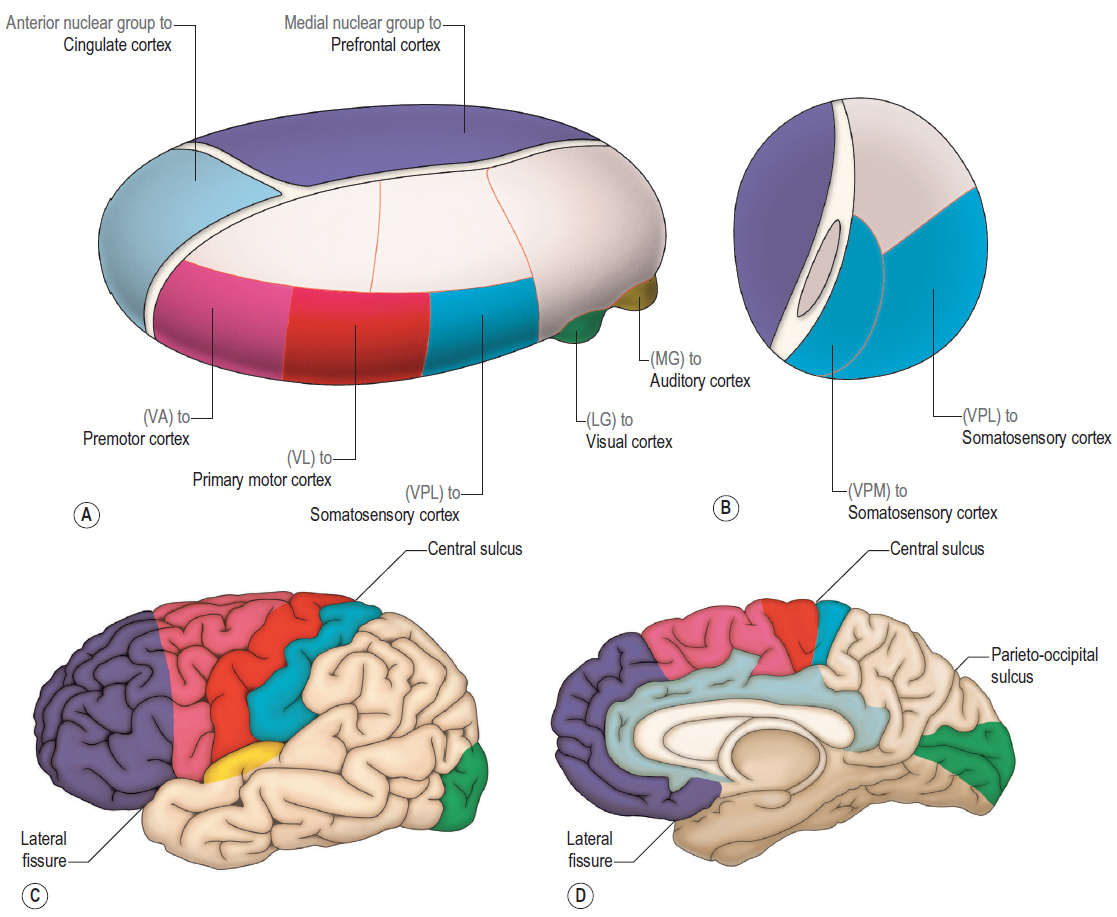
\includegraphics[width=\textwidth]{pictures/Bilder_Jule/Andere/thalamus.png}
    \caption[Projektionen thalamischer Nuclei]{\textbf{Projektionen thalamischer Nuclei.} Dargestellt sind die verschiedenen Teilbereiche des Thalamus, sowie die zugehörigen Areale der Großhirnrinde, mit denen sie in Verbindung stehen. Zum Thalamus gehören unter anderem der Corpus geniculatum mediale (MGN~- hier MG) und der Corpus geniculatum laterale (LGN~- hier LG). \textbf{A:} anterior-laterale Ansicht, \textbf{B:} Coronalschnitt, \textbf{C:} laterale Ansicht des cerebralen Cortex, \textbf{D:} mediale Aspekte des cerebralen Cortex. Die Farbgebung indiziert die Beziehungen, bzw. Projektionen zwischen den thalamischen Nuclei und den zugehörigen Arealen der Großhirnrinde.\index{Thalamus} Abbildung aus \textit{Neuroanatomy}, Crossman und Neary \textsuperscript{\cite[12]{crossman2014neuroanatomy}}.}
    \label{fig:thalamus_nuclei}
\end{figure}

\subsubsection{Subthalamus} \index{Subthalamus}
%%%%%%%%%%%%%%%%%%%%%%%%%%%%%%%%%%%%%%%%%%%%%%%%%%%%%%%%%%%

Der Subthalamus ist eine kleine Region des Diencephalons. In ihm liegt ventro-lateral der subthalamische Nucleus\index{Nucleus! subthalamicus}, direkt medial zur Capsula interna. Er zeichnet sich durch neuronale Verbindungen hin zum Globus pallidus und der Substantia nigra aus. Der subthalamische Nucleus ist an der Kontrolle von Bewegungen beteiligt \textsuperscript{\cite[12]{crossman2014neuroanatomy}} und ähnelt somit funktionell den Basalganglia (Kap.~\ref{subsec:basalganglien}) \textsuperscript{\cite[16]{crossman2014neuroanatomy}}.

\subsubsection{Hypothalamus}
\label{subsubsec:Hypothalamus} \index{Hypothalamus}
%%%%%%%%%%%%%%%%%%%%%%%%%%%%%%%%%%%%%%%%%%%%%%%%%%%%%%%%%%%

Der Hypothalamus bildet die inferiore, bzw. ventrale Wand des dritten Ventrikels, der vom Diencephalon umgeben wird (Abb.~\ref{fig:Diencephalon_Ratte}). Mittig des Hypothalamus geht das \textit{Infundibulum} hervor, das Hypothalamus und Hypophyse miteinander verbindet. Wie auch der Thalamus besteht der Hypothalamus aus mehreren kleineren Kerngebieten. Dazu gehört der \textbf{Mammillarkörper}\index{Mammillarkörper}, auch \textit{Corpus mamillare} (Abb.~\ref{fig:Diencephalon_Ratte}~A, Abb.~\ref{fig:schaf_MB}), der caudal im Hypothalamus gelegen ist und zum limbischen System gehört \textsuperscript{\cite[16]{crossman2014neuroanatomy}}. Beim Menschen, sowie bei Primaten, handelt es sich dabei um eine paarige \textsuperscript{\cite[7]{crossman2014neuroanatomy}}, bei anderen Säugetieren, wie der Ratte, um eine unpaare Struktur \textsuperscript{\cite[13]{paxinos2014rat}}. Der Mammillarkörper erhält Input aus dem Hippocampus über den Fornix (Abb.~\ref{fig:schaf_midsagittal}~B) und ist an der Regulierung des Gedächtnisses beteiligt \textsuperscript{\cite[7]{neurowissenschaften_baer}}. Des Weiteren liegen innerhalb des Hypothalamus neurosekretorische Kerngebiete und die \textbf{Neurohypophyse}\index{Hypophyse! Neurohypophyse}, sowie höhere Koordinationszentren des autonomen Systems \textsuperscript{\cite[6]{storch2012lehrbuchzoo}}.

\begin{figure}[H]
    \centering
    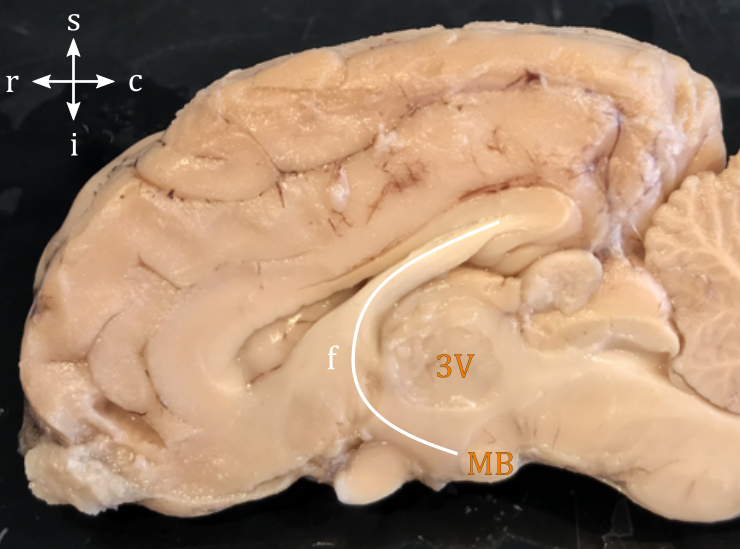
\includegraphics[width=0.5\textwidth]{pictures/Bilder_Jule/Schaf/Ausschnitte/MB.png}
    \caption[Lage der Mammillarkörper]{\textbf{Lage der Mammillarkörper.} Der Mammillarkörper (MB) befindet sich unterhalb des dritten Ventrikels (3V) und steht über den Fornix (f) mit dem Hippocampus in Verbindung.}
    \label{fig:schaf_MB}
\end{figure}{}

\noindent Im Hypothalamus gibt es Thermorezeptoren, die die lokale Temperatur im Hypothalamus wahrnehmen und bei Erwärmung Schwitzen und bei Tieren zudem Hecheln auslösen. Bei Unterkühlung wird Zittern induziert. Osmorezeptoren überwachen die Osmolarität des Blutes, Hormon-Rezeptoren können die Konzentration verschiedener Hormone messen. Dadurch können physiologische Ungleichgewichte erkannt werden, die zu somatosensorischen, vegetativen und endokrinen Reaktionen führen \textsuperscript{\cite[14]{penzlin2005tierphys}}. Beispielsweise wirkt sich die Registrierung von Hunger und Durst auf Appetit und Nahrungsaufnahme aus \textsuperscript{\cite[6]{storch2012lehrbuchzoo}}. Die vielseitigen Reaktionen, die durch den Hypothalamus gesteuert werden, sind durch seine vielseitigen Projektionen möglich. Sie enden unter anderem im Thalamus, limbischen System, der Hypophyse und dem vegetativen Nervensystem \textsuperscript{\cite[16]{crossman2014neuroanatomy}}. \\

\noindent Diese Vielseitigkeit spiegelt sich auch in den Funktionen des Hypothalamus wieder. Zum einen ist er zusammen mit der Hypophyse\index{Hypophyse! allgemein} (Hypothalamus-Hypophysen-System), für wichtige, homöostatische Funktionen des Organismus zuständig. Dazu gehört sowohl die Regulation der Körpertemperatur, als auch die des Wasser- und Ionenhaushaltes. Auch ist der Hypothalamus als höchstes Zentrum des vegetativen Nervensystems ein wichtiges Kontrollzentrum für viele Vitalfunktionen \textsuperscript{\cite[14]{penzlin2005tierphys}}. Im Allgemeinen ist er sowohl in Funktionen des autonomen Nervensystems, des limbischen Systems und des neuroendokrinen Systems involviert \textsuperscript{\cite[16]{crossman2014neuroanatomy}}.
 
\begin{figure}[H]
	    \centering
	    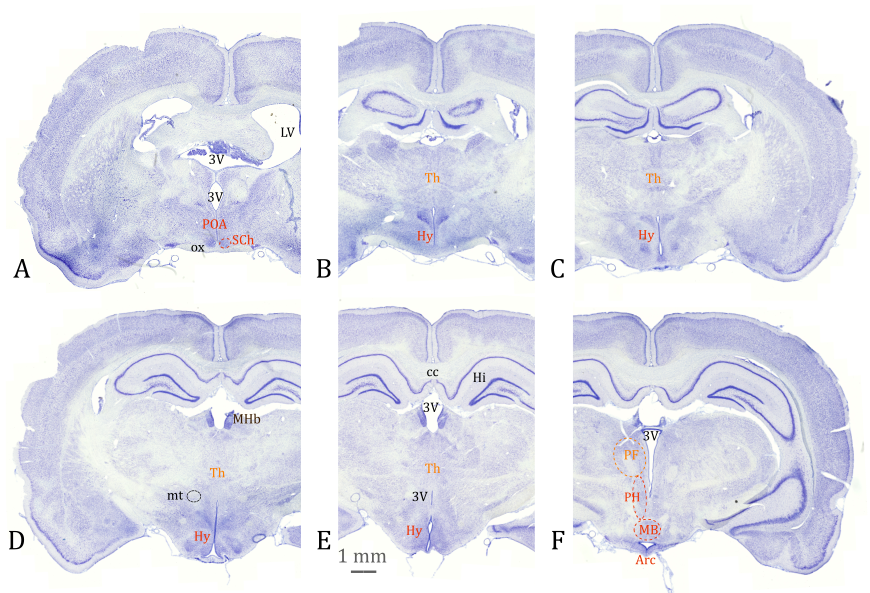
\includegraphics[width=0.99\textwidth]{pictures/Bilder_Jule/Ratte/hypothalamus.png}
	    \caption[Diencephalon Ratte]{\textbf{Diencephalon Ratte.} Gezeigt sind Coronalschnitte des Rattengehirns von rostral nach caudal (A-F: N16-1, N24-4, N24-1, N22-1, N22-1, N20-3). Bereiche des Thalamus (Th) sind in orange gekennzeichnet. Dazu gehört unter anderem der parafascikuläre thalamische Nucleus (PF). Bereiche des Hypothalamus (Hy) sind rot gekennzeichnet. Dem Hypothalamus sind der Mammillarkörper (MB), der Nucleus arcuatus (Arc), sowie der Nucleus suprachiasmaticus (SCh) und das präoptische Areal\index{präoptisches Areal} (POA) untergeordnet. Ebenfalls Teil des Diencephalons sind das optische Chiasma (ox), der dritte Ventrikel (3V), der mammillo-thalamische Trakt (mt), sowie der (mediale) Nucleus habenulares (MHb), der zum Epithalamus gehört. Ebenfalls gekennzeichnet sind Teile des Telencephalons, wie die lateralen Ventrikel (LV), der Hippocampus (Hi) und der Corpus callosum (cc).\index{Thalamus}\index{Hypothalamus}}
	    \label{fig:Diencephalon_Ratte}
\end{figure}{}



\subsection{Mesencephalon}
\label{subsec:Mesencephalon} \index{Mesencephalon}
%%%%%%%%%%%%%%%%%%%%%%%%%%%%%%%%%%%%%%%%%%%%%%%%%%%%%%%%%%%
%%%%%%%%%%%%%%%%%%%%%%%%%%%%%%%%%%%%%%%%%%%%%%%%%%%%%%%%%%%

Im Mesencephalon ist, ähnlich wie bei der Medulla und dem Rückenmark, eine funktionelle Gliederung in die motorische Grundplatte und die sensorische Flügelplatte erkennbar. Dabei sind die motorischen Kerngebiete ventral, bzw. inferior im Tegmentum gelegen. Die sensorischen Kerngebiete liegen dorsal, bzw. superior im Tectum \textsuperscript{\cite[6]{trepel2011neuroanatomie}}. Das Mesencephalon umgibt das Aquädukt des Ventrikelsystems.

\subsubsection{Tectum: Vierhügelplatte}
\index{Tectum} \index{Vierhügelplatte}
%%%%%%%%%%%%%%%%%%%%%%%%%%%%%%%%%%%%%%%%%%%%%%%%%%%%%%%%%%%
\label{subsubsec:Tectum}
Das Tectum liegt caudal des diencephalen präoptischen Areals und ist dorsal, bzw. superior im Mesencephalon lokalisiert. Es besteht aus der Vierhügelplatte, auch \textit{Lamina tecti} oder \textit{Lamina quadrigemina} genannt. Diese besteht, wie der Name impliziert, aus vier Schwellungen, den paarigen Colliculi superiores und den ebenfalls paarigen Colliculi inferiores \textsuperscript{\cite[6]{trepel2011neuroanatomie}}.

\begin{figure}[H]
    \centering
    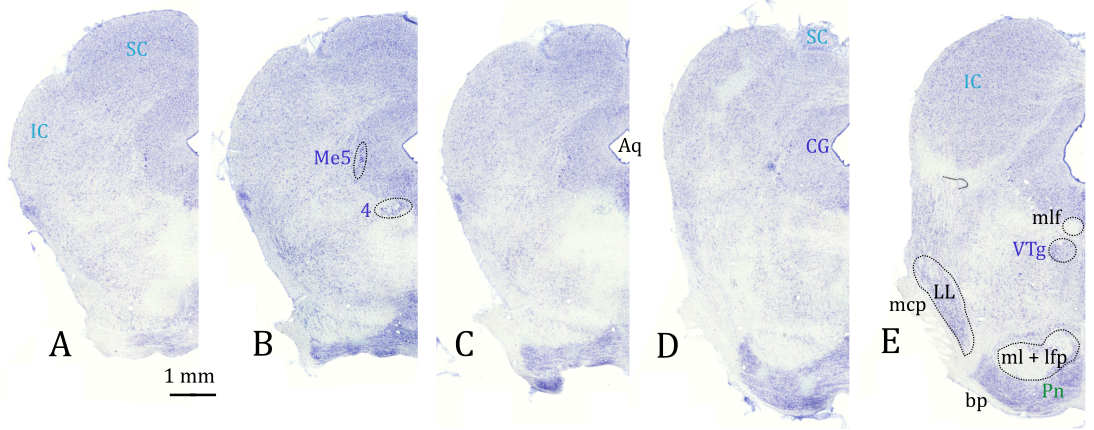
\includegraphics[width=\textwidth]{pictures/Bilder_Jule/Ratte/SC_IC.png}
    \caption[Vierhügelplatte Ratte]{\textbf{Vierhügelplatte Ratte.} Coronalschnitte von caudal nach rostral (A-E: N13-2, N14-1, N14-3, N14-4, N15-1). Teile des Cortex, die über dem Mittelhirn liegen, wurden entfernt. Bereiche des Tectums sind hellblau gekennzeichnet. Dazu gehören der Colliculus inferior (IC) und der Colliculus superior (SC). Bereiche des Tegmentums sind dunkelblau markiert. Dazu gehören das zentrale Höhlengrau (CG), der Nucleus trochlearis (4), die mesencephalen Nuclei des Nervus trigeminus (Me5), so wie der ventrale Nucleus des Tegmentums (VTg). Ebenfalls zu sehen sind das Aquädukt (Aq) des Mesencephalons und die Nuclei pontis (Pn), die dem Metencephalon zuzuordnen sind. Diese metencephalen Strukturen sind grün gekennzeichnet. Weitere Kennzeichnungen: Nuclei des lateralen Lemniscus (LL), medialer Lemniscus (ml), mediales Kleinhirn-Pedunkel (mcp), medialer longitudinaler Fasciculus (mlf), longitudinaler Fasciculus des Pons (lfp), Brachium pontis (bp). \index{Colliculus! superior} \index{Colliculus! inferior}}
    \label{fig:vierhuegelplatte_ratte}
\end{figure}{}

\noindent Die geschichteten \textbf{Colliculi superiores}\index{Colliculus! superior} enthalten wichtige Kerngebiete, die an der Entstehung und Steuerung der Augenbewegungen beteiligt sind. Über den Nervus opticus, bzw. Tractus opticus erhalten die oberen Colliculi direkte afferente Informationen von der Retina. Weitere Afferenzen kommen über den Tractus corticospinalis aus der Großhirnrinde, über den Tractus spinotectalis aus dem Rückenmark, sowie aus den Colliculi inferiores. Die efferenten Fasern aus den superioren Colliculi ziehen zu den Hirnnervenkernen (Kap.~\ref{subsec:Myelencephalon}), zur Formatio reticularis (Kap.~\ref{subsec:Hirnstamm}) und ins Rückenmark. Funktionell spielen die Colliculi superiores bei der Entstehung visueller Sakkaden, ruckartigen Bewegungen nach Fixationsphasen, eine wichtige Rolle. Auch beim  Akkommodationsreflex, der automatischen Anpassung der Linsenkrümmung um das Abbild der Außenwelt auf der Retina scharf zu stellen, könnten sie beteiligt sein. Zusammengefasst sind die Colliculi superiores in die Entstehung und Steuerung visueller Reflexe und Augenbewegungen involviert \textsuperscript{\cite[6]{trepel2011neuroanatomie}}.\\

\noindent Die \textbf{Colliculi inferiores}\index{Colliculus! inferior} liegen direkt inferior der Colliculi superiores. In ihnen werden fast alle Fasern der Hörbahn verschaltet. Somit stellen sie eine wichtige Station der Hörbahn dar (Kap.~\ref{fig:hoerbahn_pathway}). Die afferenten Fasern treffen über den lateralen Lemniscus ein. Die efferenten Fasern werden über das Brachium colliculi inferioris zum Corpus geniculatum mediale im Thalamus geleitet \textsuperscript{\cite[6]{trepel2011neuroanatomie}}.


\subsubsection{Tegmentum mesencephali}
\index{Tegmentum! mesencephali}
%%%%%%%%%%%%%%%%%%%%%%%%%%%%%%%%%%%%%%%%%%%%%%%%%%%%%%%%%%%

Der im Mesencephalon lokalisierte Teil des Tegmentums befindet sich inferior des Tectums. Es besitzt hauptsächlich motorische Funktionen. So liegen in ihm wichtige Kerngebiete des (extrapyramidalen) motorischen Systems \textsuperscript{\cite[14]{penzlin2005tierphys}}.
Auch die Kerngebiete der Hirnnerven III. (N. oculomotorius) und IV. (N. trochlearis), sowie die motorischen Kerne des Hirnnerven V. (N. trigeminus) sind im mesencephalen Tegmentum lokalisiert \textsuperscript{\cite[6]{trepel2011neuroanatomie}}.\\

\begin{figure}[H]
    \centering
    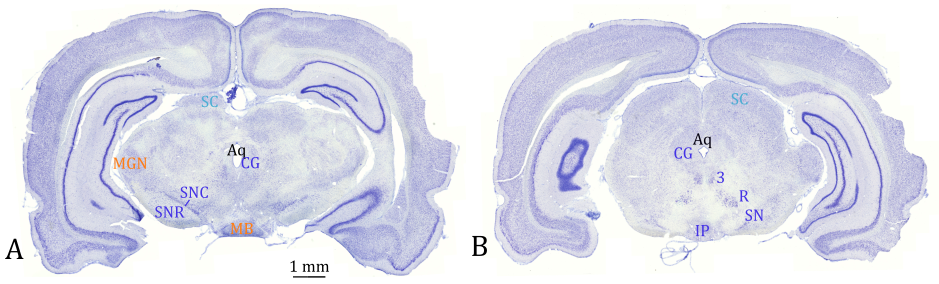
\includegraphics[width=\textwidth]{pictures/Bilder_Jule/Ratte/tegmentum_mesenc.png}
    \caption[Tegmentum Ratte]{\textbf{Tegmentum Ratte.} Coronalschnitte durch das Tegmentum mesencephali. Die Schnitte sind von rostral nach caudal angeordnet (A:~N18-4, B:~N16-2). Teilgebiete des Tegmentums sind dunkelblau gekennzeichnet. Dazu gehören das zentrale Höhlengrau (CG), das das Aquädukt (Aq) umgibt, die Substantia nigra (SN), die in die Pars compacta (SNP) und Pars reticulata (SNR) unterteilt ist, sowie der Nucleus ruber (R), die Nuclei des Nervus oculomotorius (3) und der unpaare Nucleus interpeduncularis (IP). Teilgebiete des Tectums, wie die Colliculi superiores (SC) sind hellblau markiert. Rostral sind zudem Teile des Diencephalons (orange), wie der Nucleus geniculatum mediale (MGN) und der Mammillarkörper (MB) zu sehen.}
    \label{fig:tegmentum_mesenc}
\end{figure}{}

\noindent Der \textbf{Nucleus ruber}\index{Nucleus! ruber}, ein großer, runder Komplex, ist mittig im Tegmentum mesencephali gelegen. Seine rötliche Färbung ist auf einen hohen Eisengehalt zurückzuführen. Afferenzen erhält der Nucleus ruber aus Cortex und Cerebellum. Efferenzen aus dem N. ruber ziehen über den Tractus rubrospinalis\index{Tractus! rubrospinalis} zum Rückenmark, über den Tractus rubroreticularis\index{Tractus! rubroreticularis} in die Formatio retucilaris (Kap.~\ref{subsec:Hirnstamm}) und über den Tractus rubroolivaris\index{Tractus! rubroolivaris} in die Olive. Funktionell dient der Nucleus ruber als wichtige Schaltstelle des motorischen Systems (Kap.~\ref{sec:Motorik}). Durch seine Projektionen ins Rückenmark ist er Teil des extrapyramidalmotorischen Systems \textsuperscript{\cite[6]{trepel2011neuroanatomie}}.\\

\noindent Auch die \textbf{Substantia nigra}\index{Substantia nigra}, die funktionell den Basalganglia (Kap.~\ref{subsec:basalganglien}) unterzuordnen ist, ist im Tegmentum lokalisiert. Die dunkle Farbe des Kerngebiets ist durch einen hohen Melanin-Gehalt zu erklären. Generell kann die Substantia nigra in die S.n. \textbf{pars compacta} und die S.n. \textbf{pars reticularis} unterteilt werden. Beiden sind unterschiedliche Faserverbindungen und Funktionen zuzuordnen \textsuperscript{\cite[6]{trepel2011neuroanatomie}}. 
Ausgehend von der Substantia nigra pars compacta erstrecken sich Neurone, die Dopamin enthalten, bis hin zu einer Struktur, die \textbf{Area tegmentalis ventralis (VTA)}\index{Area tegmentalis ventralis} genannt wird. Die dopaminergen Neurone der VTA sind elementarer Bestandteil des dopaminergen Systems (Kap.~\ref{dopaminerges_system}) \textsuperscript{\cite[9]{crossman2014neuroanatomy}}. Funktionell ist sie in die Kontrolle und Modulation von Bewegungsimpulsen und Bewegungsabläufen involviert. Die Degeneration dopaminerger Neurone der Substantia nigra führt zum Krankheitsbild \textbf{Morbus Parkinson}\index{Morbus Parkinson}. Folgen sind Zittern (Tremor) in Ruhephasen, erhöhter Muskeltonus in Verbindung mit steifer Muskulatur (Rigor), sowie Bewegungsarmut (Akinese) \textsuperscript{\cite[6]{trepel2011neuroanatomie}}. \\

\noindent Das \textbf{zentrale Höhlengrau}\index{zentrales Höhlengrau}, auch periaquäduktales Grau oder \textit{Griseum centrale}, ist ein dunkleres, Birnen-förmiges  Kerngebiet, das medial im Mesencephalon liegt. Es umschließt das Aquädukt ähnlich wie die graue Substanz des Rückenmarks den Zentralkanal. Etwa auf gleicher Höhe des superioren und inferioren Colliculus liegen die Nuclei des N. trochlearis und des N. oculomotorius, die äußere Augenmuskulatur innervieren und somit die Augenbewegungen steuern \textsuperscript{\cite[9]{crossman2014neuroanatomy}}. Des Weiteren ist das periaquäduktale Grau Teil des Schmerz-Systems (Kap.~\ref{subsubsec:Schmerzsinn}) \textsuperscript{\cite[25]{paxinos2014rat}}


\subsection{Basalganglia}
\label{subsec:Basalganglia} \index{Basalganglia}
%%%%%%%%%%%%%%%%%%%%%%%%%%%%%%%%%%%%%%%%%%%%%%%%%%%%%%%%%%%
%%%%%%%%%%%%%%%%%%%%%%%%%%%%%%%%%%%%%%%%%%%%%%%%%%%%%%%%%%%

Der Begriff der Basalganglia umschreibt Bestandteile des Tel-, Di- und Mesencephalons.

\begin{wrapfigure}{r}{0.44\textwidth}
    \centering
    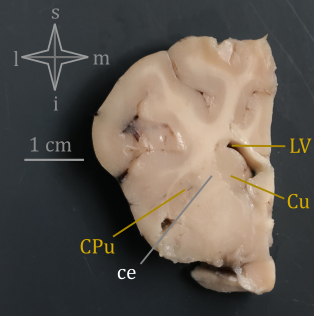
\includegraphics[width=0.42\textwidth]{pictures/Bilder_Jule/Schaf/Ausschnitte/Striatum.png}
    \caption[Striatum Schaf]{\textbf{Striatum Schaf.} Das Striatum des Schafes besteht aus dem Nucleus caudatus (Cu) und dem Putamen, bzw. Caudoputamen (CPu), die von der Capsula externa (ce), die aus vielen Fasern besteht, voneinander getrennt werden. Der Nucleus caudatus bildet die laterate Seitenwand des dritten Ventrikels (3V).}
    \label{fig:striatum}
\end{wrapfigure}

\noindent Einen Bestandteil der Basalganglia besteht aus dem \textbf{Striatum}, das sich im Telencephalon befindet und bei Säugern in \textbf{Putamen} und \textbf{Nucleus caudatus} \index{Nucleus! caudatus} unterteilt werden kann. Der Nucleus caudatus legt sich c-förmig um das Putamen, das eine platte Scheibe bildet, und folgt dabei der Oberfläche des lateralen Ventrikels, dessen Seitenwand er bildet. Vor dem Ende des Nucleus caudatus liegt die Amygdala. Auch das \textbf{Pallidum}, \textit{Globus pallidus}, das sich im Diencephalon befindet, gehört zu den Basalganglia. Durch die Capsula interna werden Putamen und Pallidum vom Thalamus getrennt (Abb.~\ref{fig:striatum}). Die Capsula interna verläuft auch zwischen dem Putamen und dem Nucleus caudatus. Die einzelnen Bestandteile der Basalganglia erhalten ihre Afferenzen unter anderem aus dem Cortex und den anderen Subbereichen der Basalganglia. Die Efferenzen verlaufen über den Thalamus. Funktionell können den Basalganglia, neben den 'klassischen Bestandteilen', auch der \textbf{Nucleus subthalamus} (Diencephalon) und die \textbf{Substantia nigra} (Mesencephalon) zugeordnet werden.
Im Allgemeinen besteht die Funktion der Basalganglia in der Regulation der Motorik (Kap.~\ref{subsec:basalganglien}) \textsuperscript{\cite[9]{trepel2011neuroanatomie}}.


\subsection{Rhombencephalon: Metencephalon}
\label{subsec:Metencephalon} \index{Metencephalon}
%%%%%%%%%%%%%%%%%%%%%%%%%%%%%%%%%%%%%%%%%%%%%%%%%%%%%%%%%%%
%%%%%%%%%%%%%%%%%%%%%%%%%%%%%%%%%%%%%%%%%%%%%%%%%%%%%%%%%%%

Das Metencephalon oder auch Hinterhirn ist Teil des Rhombencephalons (Rautenhirn). In seiner Struktur ähnelt es dem Myelencephalon und Rückenmark. Zwischen Pons und Cerebellum, die beide im Metencephalon lokalisiert sind, verläuft der vierte Ventrikel.


\subsubsection{Pons}
\label{subsubsec:Pons} \index{Pons}
%%%%%%%%%%%%%%%%%%%%%%%%%%%%%%%%%%%%%%%%%%%%%%%%%%%%%%%%%%%

Der Pons oder das Brückenhirn beschreibt jenen Teil des Metencephalons, der direkt zwischen Mes- und Myelencephalon und inferior des Cerebellums liegt. Der Pons bildet einen von Außen gut sichtbaren, dicken Wulst, der aus vielen Fasern, aber auch aus grauer Substanz besteht. Im inferioren, bzw. ventralen Bereich, der sogenannten \textbf{Brückenhaube}, liegt das Tegmentum\index{Tegmentum! pontine}, in dem einige Hirnnervenkerne lokalisiert sind. Dazu gehören der Nucleus des N. abducens und des N. facialis. Auch die Nuclei des Trapezkörpers und des medialen Lemniscus sind dort lokalisiert.

\begin{figure}[H]
    \centering
    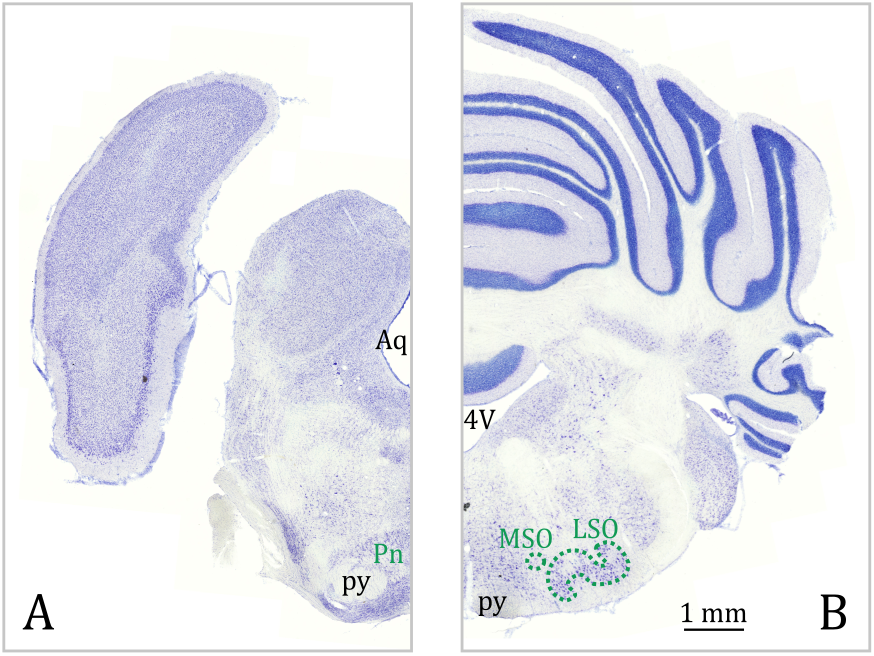
\includegraphics[width=0.7\textwidth]{pictures/Bilder_Jule/Ratte/pons.png}
    \caption[Pons Ratte]{\textbf{Pons Ratte.} Dargestellt sind ein rostraler (A:~N12-2) und caudaler (B:~N08-2) Querschnitt durch den Pons. Dabei ist rostral über dem Pons noch das Mesencephalon zu sehen, in dem sich das Aquädukt (Aq) befindet. Über dem Mesencephalon sind Teile des Cortex sichtbar. In diesem Bereich des Pons befinden sich die Nuclei pontis (Pn). Im caudalen Querschnitt ist am oberen Ende das Cerebellum sichtbar. Auch der vierte Ventrikel (4V) ist zu sehen, sowie die mediale (MSO) und laterale obere Olive (LSO). Die Pyramidenbahn (py) liegt im ventralen Bereich des Pons und erstreckt sich über dessen gesamte Länge.}
    \label{fig:pons_ratte}
\end{figure}{}

\noindent Der superiore Bereich wird auch \textbf{Brückenbasis} genannt. Sie beinhaltet die \textbf{Pyramidenbahn} und den \textbf{oberen Olivenkomplex}\index{Olive! obere Olive} (\textit{Nucleus olivaris superior}), der eine wichtige Station der Hörbahn darstellt. Ebenfalls im Pons liegen die \textbf{Nuclei pontis}\index{Nuclei! pontis}, auch Brückenkerne genannt. Diese Nuclei sind von den Fasermassen, die ihnen entspringen, bzw. zu ihnen führen, umgeben. Die meisten Afferenzen erhalten sie über den Tractus corticopontinus\index{Tractus! corticopontinus}. Dieser Trakt führt Fasern aus diversen Großhirnbereichen. Dabei erhalten die Nuclei unter anderem Informationen über Bewegungsentwürfe, die im prämotorischen Cortex ausgearbeitet werden. Nach dem die Fasern innerhalb des Pons auf die contralaterale Seite kreuzen, enden die Efferenzen in der contralateralen Kleinhirnhemisphäre. So können die Nuclei pontis die erhaltenen Informationen zur weiteren Feinabstimmung an das Kleinhirn weiterleiten. Die Nuclei pontis spielen somit eine entscheidende Rolle  bei der Verschaltung von Informationen aus dem Großhirn zum Kleinhirn \textsuperscript{\cite[5]{trepel2011neuroanatomie}}.

\subsubsection{Cerebellum}
\label{subsubsec:Cerebellum} \index{Cerebellum! allgemein}
%%%%%%%%%%%%%%%%%%%%%%%%%%%%%%%%%%%%%%%%%%%%%%%%%%%%%%%%%%%

Das Cerebellum oder Kleinhirn ist dorsal oder superior im Metencephalon, über dem Hirnstamm, gelegen. Somit bedeckt es dorsal den vierten Ventrikel. Es ist durch drei Kleinhirnstiele, die \textit{Pedunculi cerebellaris}\index{Kleinhirnpedunkel}, mit dem Hirnstamm verbunden. Über diese Stiele verlaufen sowohl die Afferenzen als auch die Efferenzen des Cerebellums. Zudem ziehen zwei Kleinhirnsegel (\textit{Velum})\index{Velum} zum Mesencephalon und der Medulla. Diese Veli bestehen aus weißer Substanz und bilden das Dach des vierten Ventrikels. Bei lissencephalen\index{lissencephal} Spezies weist das Cerebellum, ähnlich wie die Großhirnrinde, viele Faltungen auf. Im direkten Vergleich sind die Falten des Cerebellums deutlich kleiner und zahlreicher. Sie verlaufen horizontal und werden auch als Blätter (\textit{Foliae}) bezeichnet \textsuperscript{\cite[7]{trepel2011neuroanatomie}}. Eine weitere Ähnlichkeit zum Cortex besteht in der Schichtung des Cerebellums. Wie Teile der  Großhirnrinde ist auch das Kleinhirn aus drei Zellschichten aufgebaut. Die äußerste Schicht ist die \textbf{Molekularschicht} unter der die \textbf{Purkinje-Zellschicht} liegt. Die innerste Schicht ist die \textbf{Körnerzellschicht} (Abb.~\ref{fig:cerebellum_ratte}) \textsuperscript{\cite[14]{penzlin2005tierphys}}.

\begin{figure}[H]
    \centering
    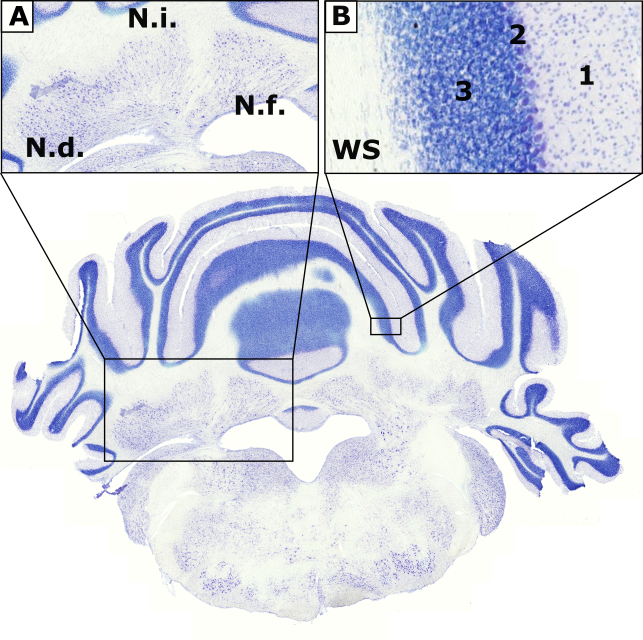
\includegraphics[width=\textwidth]{pictures/Bilder_Jule/Ratte/cerebellum.png}
    \caption[Schichtung Cerebellum]{\textbf{Schichtung Cerebellum.} Ausschnitt des caudalen Cerebellums, unter dem sich die Medulla befindet (N04-1). Zwischen Medulla und Cerebellum ist der vierte Ventrikel sichtbar. Gekennzeichnet sind die weiße Substanz (WS), sowie die drei Schichten der grauen Substanz. Die äußerste Schicht ist die Molekularschicht (\textbf{1}). Weiter innen liegen die Purkinje-Zellschicht (\textbf{2}) und die Körnerzellschicht (\textbf{3}).}
    \label{fig:cerebellum_ratte}
\end{figure}

\noindent Aufgrund der verschiedenen afferenten Faserverbindungen lässt sich das Cerebellum in drei Gebiete gliedern: Das \textbf{Vestibulocerebellum}\index{Cerebellum! Vestibulocerebellum} erhält Afferenzen aus aus dem Vestibularapparat des Innenohrs, das \textbf{Spinocerebellum}\index{Cerebellum! Spinocerebellum} aus dem Rückenmark und das \textbf{Corticocerebellum}\index{Cerebellum! Corticocerebellum} aus den Nuclei pontis. Des Weiteren liegen im Cerebellum die \textbf{Kleinhirnkerne}, zu denen der Nucleus dentatus, der Nucleus emboliformis, sowie der Nucleus globosus und der Nucleus fastigii gehören. Das Cerebellum spielt eine wichtige Rolle für die Koordination von Haltung und Bewegung und gilt generell als motorisches Koordinationszentrum (Kap.~\ref{sub:kleinhirn}) \textsuperscript{\cite[7]{trepel2011neuroanatomie}}.

\subsection{Rhomencephalon: Myelencephalon}
\label{subsec:Myelencephalon} \index{Myelencephalon}
%%%%%%%%%%%%%%%%%%%%%%%%%%%%%%%%%%%%%%%%%%%%%%%%%%%%%%%%%%%
%%%%%%%%%%%%%%%%%%%%%%%%%%%%%%%%%%%%%%%%%%%%%%%%%%%%%%%%%%%

\subsubsection{Medulla} \index{Medulla oblongata}
%%%%%%%%%%%%%%%%%%%%%%%%%%%%%%%%%%%%%%%%%%%%%%%%%%%%%%%%%%%

Das Myelencephalon (Nachhirn) besteht aus der \textbf{Medulla oblongata}, auch verlängertes Rückenmark genannt. Sein 'Dach' ist dünn und weist kleine Falten auf \textsuperscript{\cite[6]{storch2012lehrbuchzoo}}. Die Medulla liegt caudal des Pons und leitet zum Rückenmark über, dem es sowohl in Aufbau als auch Funktion ähnelt (Abb.~\ref{fig:medulla_schema},~\ref{fig:ruckenmark_schema}). Genau wie im Rückenmark sind die sensorischen Regionen dorsal im Hinterhorn (Flügelplatte) und die motorischen Regionen ventral im Vorderhorn (Grundplatte) in der grauen Substanz lokalisiert. Dabei liegen die somatosensorischen Regionen eher lateral und die viscerosensorischen Regionen eher medial. Im Vergleich zum Rückenmark ist der Zentralkanal erweitert und bildet den vierten Ventrikel. Beim Übergang von Rückenmark zur Medulla geht die dorso-ventrale Organisation des Rückenmarks in eine eher medio-laterale Organisation über \textsuperscript{\cite[14]{penzlin2005tierphys}}.

\begin{figure}[H]
    \centering
    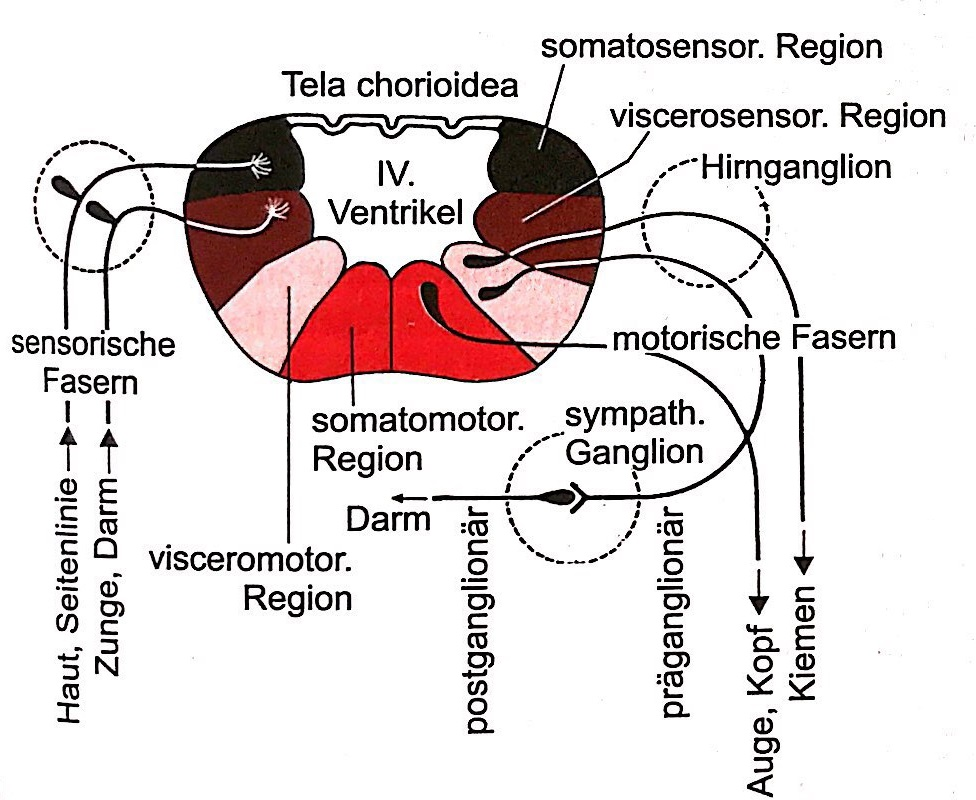
\includegraphics[width=0.6\textwidth]{pictures/Bilder_Jule/Andere/medulla_schema.jpg}
    \caption[Aufbau der Medulla]{\textbf{Aufbau der Medulla.} Gezeigt ist ein schematischer Querschnitt durch die Medulla, bzw. den Hirnstamm. Die superiore, bzw. dorsale, sensorische Seite ist nach oben, die inferiore, bzw. ventrale, motorische Seite nach unten orientiert.\\
    Abbildung aus \textit{Lehrbuch der Tierphysiologie}, Penzlin {\textsuperscript{\cite[14]{penzlin2005tierphys}}}.}
    \label{fig:medulla_schema}
\end{figure}{}

\noindent Im Vergleich zu den anderen Hirnarealen entspringen der Medulla die meisten Hirnnerven (Abb.~\ref{fig:hirnnerven_schaf}). So liegen sowohl die primären sensorischen, als auch die primären motorischen Kerngebiete der Hirnnerven IV bis XII in der Medulla \textsuperscript{\cite[14]{penzlin2005tierphys}}. Neben zahlreichen Hirnnervenkernen ist auch die \textbf{inferiore Olive}\index{Olive! untere Olive}, ein Kerngebiet, das in die Motorkontrolle involviert ist (Kap.~\ref{sec:Motorik})  \textsuperscript{\cite[9]{crossman2014neuroanatomy}}, in der Medulla lokalisiert. Auch die Hinterstrangkerne, der \textbf{Nucleus cuneatus}\index{Nucleus! cuneatus} und der \textbf{Nucleus gracilis}\index{Nucleus! gracilis}, die Stationen der somatosensorischen Bahn darstellen (Kap.~\ref{subsubsec:tastsinn}) \textsuperscript{\cite[5]{trepel2011neuroanatomie}} und der cochleare Nucleus\index{Nucleus! cochlearis}, sind in der Medulla lokalisiert (Abb.~\ref{fig:medulla_ratte}). Zusammen mit dem Pons\index{Pons} besteht die Funktion des Myelencephalon unter anderem in der Regulation von Atmung und Kreislauf \textsuperscript{\cite[14]{penzlin2005tierphys}}.

\begin{figure}[H]
    \centering
    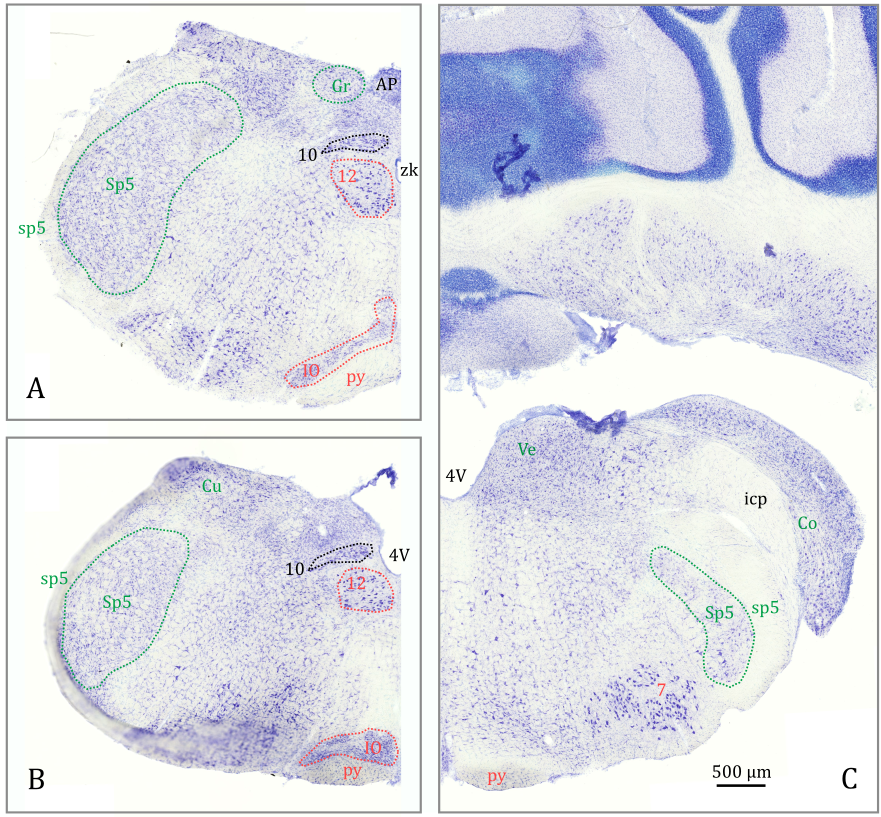
\includegraphics[width=\textwidth]{pictures/Bilder_Jule/Ratte/medulla.png}
    \caption[Medulla Ratte]{\textbf{Medulla Ratte.} Gezeigt sind Querschnitte durch die Medulla. \textbf{A} ist caudaler (N01-4), \textbf{B} rostraler (N02-4) lokalisiert. Auf \textbf{C}, dass sich weiter rostral befindet (N6-1) ist oben bereits das Cerebellum sichtbar. Sensorische Gebiete sind grün gekennzeichnet. Dazu gehören der Spinalkanal des N. trigeminus (sp5), sowie die zugehörigen Nuclei (Sp5), der Nucleus cochlearis (Co), der Nucleus vestibularis (Ve), sowie die Hinterstrangkerne: der Nucleus cuneatus (Cu) und der Nucleus gracilis (Gr). Motorische Gebiete sind rot markiert. Dazu gehören die Nuclei des N. hypoglossus (12), die Pyramidenbahn (py) und die inferiore Olive (IO). Ebenfalls gekennzeichnet sind die Nuclei des Vagus Nervs (10), der sowohl sensorische als auch motorische Funktionen besitzt, das Pedunculus cerebellaris inferior (icp), der Zentralkanal (zk) und der vierte Ventrikel (4V).} 
    \label{fig:medulla_ratte}
\end{figure}{}


\subsection{Hirnstamm}
\label{subsec:Hirnstamm} \index{Hirnstamm}
%%%%%%%%%%%%%%%%%%%%%%%%%%%%%%%%%%%%%%%%%%%%%%%%%%%%%%%%%%%
%%%%%%%%%%%%%%%%%%%%%%%%%%%%%%%%%%%%%%%%%%%%%%%%%%%%%%%%%%%

Unter dem Begriff Hirnstamm (\textit{Truncus cerebri}) werden die ventralen Bereiche des Mittelhirns (Mesencephalon), des Hinterhirns (Metencephalon) und des Nachhirns (Myelencephalon) zusammengefasst. Es besteht somit aus Teilen des Mittelhirns, sowie aus dem Pons und der Medulla. Rostral, vor dem Hirnstamm, liegt das Zwischenhirn (Diencephalon), caudal, hinter dem Hirnstamm, folgt das Rückenmark. Im Hirnstamm sind motorische Zentren lokalisiert, die für die Kontrolle der Körperhaltung und Bewegung zuständig sind. Diese Bereiche werden im Allgemeinen auch als \textbf{Tegmentum} bezeichnet. Es kann, dem Verlauf des Ventrikelsystems folgend, in drei Unterbereiche gegliedert werden: Das \textit{Tegmentum mesencephali}\index{Tegmentum! mesencephali} befindet sich im ventralen, bzw. inferioren Mittelhirn \textsuperscript{\cite[6]{trepel2011neuroanatomie}}. Das \textit{Tegmentum pontine}\index{Tegmentum! mesencephali} ist ebenfalls ventral gelegen und befindet sich im Pons. Der Bereich des Tegmentums, der sich in der Medulla befindet, wird \textit{Tegmentum myelencephali}\index{Tegmentum! myelencephali} genannt. Im Vergleich zum Mes- und Metencephalon ist das Tegmentum im Myelencephalon dorsal, bzw. superior gelegen \textsuperscript{\cite[5]{trepel2011neuroanatomie}}.\\

\noindent Neben den motorischen Funktionen besitzt der Hirnstamm auch andere Aufgaben. So liegen in ihm auch relativ autonome, vegetative Zentren, die beispielsweise Atem- und Kreislaufsystem steuern \textsuperscript{\cite[14]{penzlin2005tierphys}}. Eines dieser Zentren ist die \textbf{Formatio reticularis}\index{Formatio reticularis}. Sie erstreckt sich vom Mesencephalon über den Pons und die Medulla bis hinab ins Rückenmark. Durch die Formatio reticularis werden sowohl sympathische als auch parasympathische Zentren gesteuert. Sie selbst wird vom Hypothalamus kontrolliert. Funktionell lässt sich die Formatio reticularis in eine Vielzahl kleinerer Zentren unterteilen. Sowohl motorische Zentren, wie das sogenannte motorische Zentrum und das Augenbewegungszentrum (Kap.~\ref{sec:Motorik}), als auch Kreislauf- und Atemzentren sind in ihr lokalisiert. Des Weiteren beinhaltet sie das sogenannte Brechzentrum und das Miktionszentrum \textsuperscript{\cite[6]{trepel2011neuroanatomie}}.


\subsection{Rückenmark}
\label{subsec:Rueckenmark} \index{Rückenmark}
%%%%%%%%%%%%%%%%%%%%%%%%%%%%%%%%%%%%%%%%%%%%%%%%%%%%%%%%%%%
%%%%%%%%%%%%%%%%%%%%%%%%%%%%%%%%%%%%%%%%%%%%%%%%%%%%%%%%%%%

Das Rückenmark zeigt eine dorso-ventrale Organisation auf (Abb.~\ref{fig:ruckenmark_schema}). Dabei weist die zentral gelegene \textbf{graue Substanz}\index{graue Substanz}, die den Zentralkanal umgibt und die Somata der vorliegenden Neurone enthält, eine typische Schmetterlingsform auf. Generell kann zwischen dem Vorder- und Hinterhorn des Rückenmarks unterschieden werden. Im ventralen Vorderhorn (Grundplatte) sind die Somata der motorischen Fasern lokalisiert. Dabei sind die somatomotorischen Neurone eher dorsal, die visceromotorischen eher dorso-lateral gelegen. Im dorsalen Hinterhorn (Flügelplatte), in dem die Somata der sensorischen Neurone liegen, sind die somatosensorischen Neurone eher ventral gelegen, die viscerosensorischen eher dorsal.\\

\noindent Die \textbf{weiße Substanz}\index{weiße Substanz} umgibt peripher die graue Substanz. Sie enthält neben Gliazellen und Blutgefäßen ausschließlich markhaltige Fasern. Dabei verlaufen sowohl die aufsteigenden, als auch die absteigenden Bahnen in der weißen Substanz. Des Weiteren treten pro Körpersegment jeweils zwei laterale Nerven aus, die \textbf{dorsale und ventrale Wurzel} genannt werden (Abb.~\ref{fig:ruckenmark_schema}). Diese vereinen sich in kurzem Abstand zum Rückenmark zu \textbf{Spinalnerven}. Kurz vor dieser Vereinigung von dorsaler und ventraler Wurzel ist eine Schwellung erkennbar, das sogenannte \textbf{Spinalganglion}. Dieses dient der metabolischen Versorgung, sowie der Energieversorgung der vorliegenden Neurone. Nach der Vereinigung zum Spinalnerv spaltet sich dieser erneut in drei Äste (Rami) auf (Abb.~\ref{fig:ruckenmark_wirbelsaeule}) \textsuperscript{\cite[14]{penzlin2005tierphys}}.

\begin{figure}[H]
     \centering
     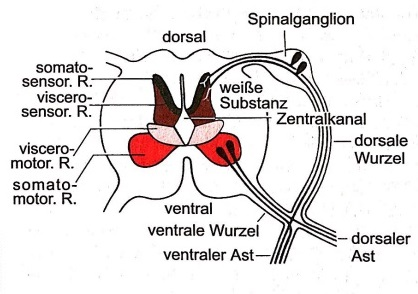
\includegraphics[width=0.59\textwidth]{pictures/Bilder_Jule/Andere/rueckenmark_schema.jpg}
     \caption[Aufbau des Rückenmarks]{\textbf{Aufbau des Rückenmarks.} Gezeigt ist ein schematischer Querschnitt durch das Rückenmark. Das dorsale Hinterhirn liegt oben, das ventrale Vorderhorn unten. Abbildung aus \textit{Lehrbuch der Tierphysiologie}, Penzlin \textsuperscript{\cite[14]{penzlin2005tierphys}}.}
     \label{fig:ruckenmark_schema}
 \end{figure}{}

\noindent Innerhalb der Wirbelsäule ist das Rückenmark, wie auch das Gehirn innerhalb des Schädel-knochens, von mehreren Hüllen umgeben. Bei der innersten, ersten Schicht handelt es sich um die weiche \textbf{Pia mater}\index{Hirnhäute}. Zwischen der weichen Pia mater und der äußeren, festeren \textbf{Dura mater spinalis} befindet sich der \textbf{Subarachnoidalraum}, der mit Liquor gefüllt ist. Das Rückenmark ist an mehreren seitlichen Bändern, den \textbf{Ligamenta denticulatum}, im Subarachnoidalraum befestigt, bzw. aufgehängt (Abb.~\ref{fig:ruckenmark_wirbelsaeule}). 

\begin{figure}[H]
     \centering
     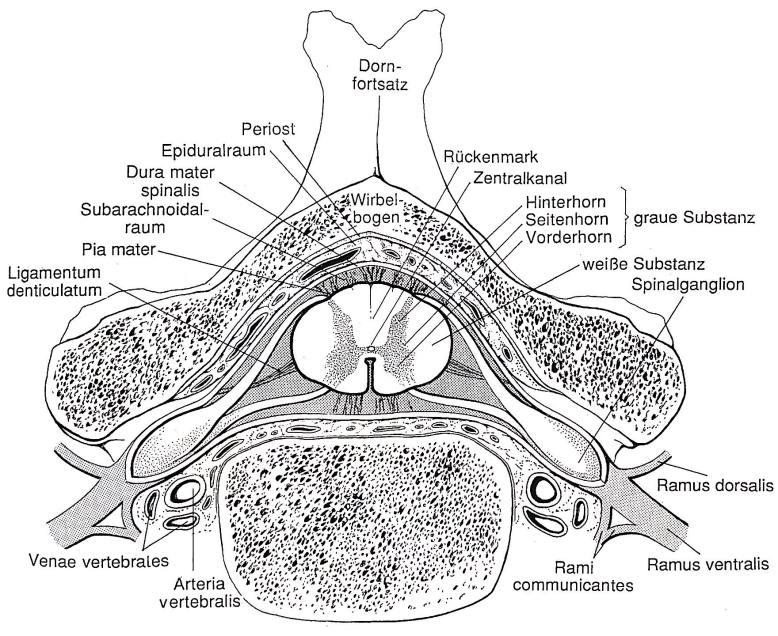
\includegraphics[width=0.79\textwidth]{pictures/Bilder_Jule/Andere/rueckenmark_wirbelsaeule.png}
     \caption[Querschnitt durch Wirbelsäule und Rückenmark]{\textbf{Querschnitt durch Wirbelsäule und Rückenmark.} Aufhängung des Rückenmarks innerhalb der Wirbelsäule eines höheren Primaten. Die dorsale Seite ist nach oben, die ventrale nach unten orientiert.\\
     Abbildung aus \textit{Kurzes Lehrbuch der Zoologie}, Storch und Welsch \textsuperscript{\cite[6]{storch2012lehrbuchzoo}}.}
     \label{fig:ruckenmark_wirbelsaeule}
\end{figure}


\subsection{Hirnnerven}
\label{subsec:Hirnnnerven}
\index{Hirnnerven! allgemein}
%%%%%%%%%%%%%%%%%%%%%%%%%%%%%%%%%%%%%%%%%%%%%%%%%%%%%%%%%%%
%%%%%%%%%%%%%%%%%%%%%%%%%%%%%%%%%%%%%%%%%%%%%%%%%%%%%%%%%%%

Zwischen dem Gehirn und den peripheren Strukturen verlaufen insgesamt zwölf Hirnnerven. Diese bilateralen, gepaarten Nerven beinhalten sowohl afferente als auch efferente Fasern. Die Nummerierung der Hirnnerven verläuft von rostral nach caudal. Die ersten beiden Hirnnerven liegen am Vorderhirn. Der \textbf{N. olfactorius (I)}\index{Hirnnerven! 01. N. olfactorius} beinhaltet sensorische Fasern, die Information aus dem Riechepithel zum Bulbus olfactorius weiterleiten. Er ist wesentlicher Bestandteil des Geruchssinns. Der zweite Hirnnerv, der \textbf{N. opticus (II)}\index{Hirnnerven! 02. N. opticus} beinhaltet ebenfalls ausschließlich sensorische Fasern. Diese leiten Informationen aus der Retina zum Nucleus geniculatum laterale weiter. Der N. opticus ermöglicht das Sehen und ist zudem am Pupillenreflex beteiligt. Die restlichen Hirnnerven sind am Hirnstamm lokalisiert (Abb.~\ref{fig:hirnnerven_schaf}) \textsuperscript{\cite[10]{crossman2014neuroanatomy}}. \\

\noindent Der \textbf{N. oculomotorius (III)}\index{Hirnnerven! 03. N. oculomotorius} beinhaltet sowohl motorische als auch parasympathische Fasern. Die motorischen Fasern innervieren extraokulare Muskeln, die die Augenbewegungen steuern, wie den superioren, inferioren und medialen Musculus rectus. Der Großteil dieser motorischen Fasern entspringt dem Nucleus oculomotorius, der sich im Mesencephalon etwa auf Höhe des Colliculus superior befindet. Über den N. oculomotorius werden Augenbewegungen gesteuert, sowie das Anheben des oberen Augenlids. Die parasympathischen Fasern des N. oculomotorius erhalten Informationen aus dem Edinger-Westphal Nucleus (\textit{Nucleus accessorius nervi oculomotorii}). Diese Fasern innervieren den Musculus sphincter pupillae, den Ringmuskel des Auges, der die Pupille verengt, sowie den Ziliarmuskel des Auges, der an Augenbewegungen beteiligt ist. Durch diese Verbindung ist der N. oculomotor auch auch an der Pupillenkontraktion und der Pupillenakkommodierung beteiligt. Ähnlich wie der N. opticus ist auch der \textbf{N. trochlearis (IV)}\index{Hirnnerven! 04. N. trochlearis} funktionell für die Augenbewegungen zuständig. Er enthält motorische Fasern, die vom Nucleus trochlearis zum Musculus obliquus superior der äußeren Augenmuskulatur ziehen. Der \textbf{N. trigeminus (V)}\index{Hirnnerven! 05. N. trigeminus} enthält sowohl motorische als auch sensorische Fasern. Die sensorischen Fasern enthalten Informationen aus Gesicht, Kopfhaut, Augenhornhaut, Nasen- und Mundhöhle, sowie der Dura mater des Schädels. Diese Informationen werden zum sensorischen Nucleus des Trigeminus weitergeleitet. Die Funktion des sensorischen fünften Hirnnerven besteht in der Sinneswahrnehmung des Kopfes. Die motorischen Fasern dieses Nervs ziehen von den Motornuclei zu den Musculi masticatorii (Kaumuskulatur) und dem Musculus tensor tympani (Spanner des Trommelfell). Durch diese Projektionen ist der N. trigeminus in das Öffnen und Schließen des Mundes, sowie in die Spannung des Trommelfells involviert. Ein weiterer Hirnnerv, der in die Augenbewegung involviert ist, ist der \textbf{N. abducens (VI)}\index{Hirnnerven! 06. N. abducens}. Er führt motorische Fasern, die vom Nucleus abducens aus dem caudalen Pons zum lateralen Musculus rectus ziehen. Im \textbf{N. facialis (VII)}\index{Hirnnerven! 07. N. facialis} verlaufen sowohl sensorische, motorische und parasympathische Fasern. Die sensorischen Fasern entspringen dem anterior gelegenen Zweidrittel der Zunge und enden im Nucleus solitarius. Diese sensorischen Fasern sind für den Geschmackssinn verantwortlich. 
Ein Teil der motorischen Fasern des Facialis verläuft vom Nucleus facialis zum Musculus stapedius, der am Stapediusreflex beteiligt ist. Dadurch kann die Spannung der Mittelohrmuskulatur reguliert werden. Andere motorische Fasern enden an jenen Muskeln, die für die Mimik zuständig sind.  Die parasympathischen Fasern des N. facialis sind für den Speichel- und Tränenfluss verantwortlich. Sie ziehen vom superioren Nucleus salivatorius zu den Speichel- und Tränendrüsen. Der achte Hirnnerv, der \textbf{N. vestibulocochlearis (VIII)}\index{Hirnnerven! 08. N. vestibulocochlearis} enthält sensorische Fasern. Diese ziehen vom Vestibularorgan und der Cochlea zu den Nuclei vestibularis, bzw. den Nuclei cochlearis. Funktionell ist der N. Vestibulocochlearis für den Gleichgewichts- und Hörsinn verantwortlich. Der \textbf{N. glossopharyngeus (IX)}\index{Hirnnerven! 09. N. glossopharyngeus} beinhaltet sensorische, motorische und 

\begin{figure}[H]
    \centering
    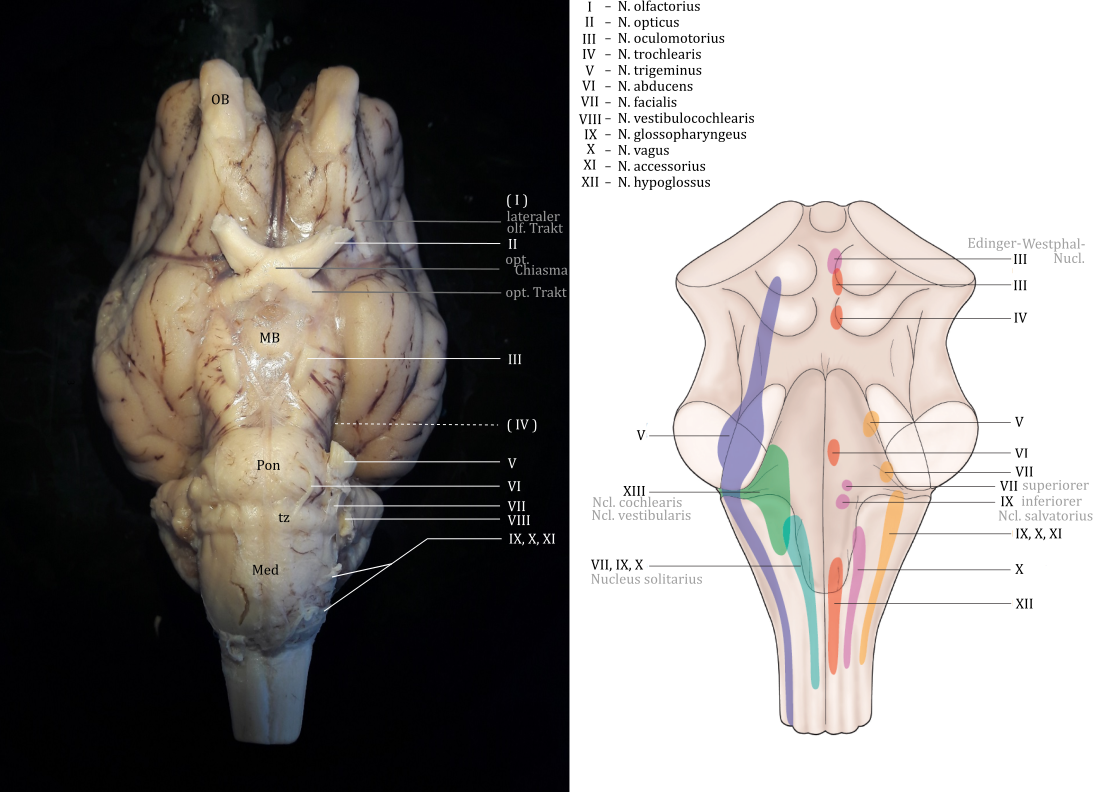
\includegraphics[width=\textwidth]{pictures/Bilder_Jule/Schaf/Aussenansicht/Hirnnerven.png}
    \caption[Hirnnerven Schaf]{\textbf{Hirnnerven Schaf.} \textbf{LINKS:} Ventralansicht des Schafshirn. Gekennzeichnet sind die Hirnnervenkerne. Der Bulbus olfactorius (OB), der Mammillarkörper (MB), der Pons (Pon), der Trapezkörper (tz), sowie die Medulla (Med) sind ebenfalls gekennzeichnet. Da der N. trochlearis nicht sichtbar ist, ist lediglich seine ungefähre Position markiert. \textbf{RECHTS:} dorsale Ansicht des Hirnstamms des Schafs. Markiert sind die Nuclei der Hirnnerven. Dabei sind die sensorischen Kerngebiete links, die motorischen rechts gekennzeichnet. Abbildung nach \textit{Neuroanatomy}, Crossman und Neary \textsuperscript{\cite[10]{crossman2014neuroanatomy}}.}
    \label{fig:hirnnerven_schaf}
\end{figure}

parasympathische Fasern. Ein Teil der sensorischen Fasern ist an der allgemeinen Sinneswahrnehmung beteiligt. Sie ziehen aus dem Pharynx, dem posterioren Drittel der Zunge, der Eustachischen Röhre und dem Mittelohr zum sensorischen Nucleus des Trigeminus. Ein weiterer Teil der sensorischen Fasern ist speziell für den Geschmackssinn, Chemorezeption und Druckrezeption verantwortlich. Diese Fasern entspringen unter anderem dem posterioren Drittel der Zunge, sowie dem Sinus caroticus, einer Gefäßerweiterung, die mittels Druckrezeptoren bei der Regulation des Blutdrucks mitwirkt. Die motorischen Fasern des N. glossopharyngeus entspringen dem Nucleus ambiguus und enden im Musculus stylopharyngeus, der für das Schlucken zuständig ist. Ähnlich wie die parasympathischen Fasern des N. facialis sind die parasympathischen Fasern des N. glossopharyngeal ebenfalls am Speichelfluss beteiligt. Sie ziehen vom inferioren Nucleus salivatorius zur Ohrspeicheldrüse (Glandula parotis). Auch der zehnte Hirnnerv, der \textbf{N. vagus (X)}\index{Hirnnerven! 10. N. vagus}, führt alle drei Fasertypen. Die sensorischen Fasern ziehen dabei teilweise, ähnlich wie die Fasern des IX, aus Rachen (Pharynx), Kehlkopf (Larynx), Luftröhre (Trachea), Speiseröhre (Oesophagus) und dem Außenohr zum sensorischen Nucleus des Trigeminus. Diese Fasern sind funktionell in die allgemeine Sinneswahrnehmung involviert. Ein anderer Teil der sensorischen Fasern des Vagusnervs entspringt den Eingeweiden in Thorax und Abdomen, dem Glomus aorticum, und dem Aortenbogen (Arcus aortae). Diese sensorischen Fasern enden im Nucleus solitarius und sind für die viszerale Sinneswahrnehmung, bzw. Chemo- und Druckrezeption zuständig. Die motorischen Fasern des N. vagus entspringen dem Nucleus ambiguus und führen wiederum zum Gaumensegel (Velum palatinum), Pharynx, Larynx und oberen Oesophagus. Ihre Funktion besteht im Schlucken und Sprechen. Die im Vagusnerv enthaltenen parasympathischen Fasern verlaufen vom dorsalen Motornucleus des Vagusnervs zu dem thorakalen und abdominalen Eingeweiden. Diese Fasern sind für die Innervation der Herzmuskulatur (Myokard), der Drüsen des Herzkreislaufsystems, sowie der Atemwege und des Magen-Darm-Trakts zuständig. Der \textbf{N. accessorius (XI)}\index{Hirnnerven! 11. N. accessorius} führt ausschließlich motorische Fasern, die den Musculus sternocleidomastoideus ('Kopfnicker') der Halsmuskulatur und den Musculus trapezius der Schultermuskulatur innerviert. Er ist für die Bewegung von Hals und Schultern zuständig. Der N. accessorius weißt eine starke Verbindung zum Rückenmark auf. Der letzte Hirnnerv, der \textbf{N. hypoglossus (XII)}\index{Hirnnerven! 12. N. hypoglossus}, enthält ebenfalls Motorneurone. Diese innervieren, vom Nucleus hypoglossus ausgehend, die innere und äußere Zungenmuskulatur. Dadurch ist er funktionell für die Bewegung der Zunge zuständig \textsuperscript{\cite[10]{crossman2014neuroanatomy}}.


\subsection{Externe Merkmale des Gehirns}
\label{subsec:Externe_Merkmale}
%%%%%%%%%%%%%%%%%%%%%%%%%%%%%%%%%%%%%%%%%%%%%%%%%%%%%%%%%%%
%%%%%%%%%%%%%%%%%%%%%%%%%%%%%%%%%%%%%%%%%%%%%%%%%%%%%%%%%%%

\subsubsection{Hirnhäute} \index{Hirnhäute}
%%%%%%%%%%%%%%%%%%%%%%%%%%%%%%%%%%%%%%%%%%%%%%%%%%%%%%%%%%%

Drei Hirnhäute liegen zwischen dem Gehirn und dem Schädelknochen (Abb.~\ref{fig:hirnhaeute}). Die äußerste Schicht ist die \textbf{Dura mater}, auch harte Hirnhaut genannt. Sie ist lederartig, unelatisch und fest und umgibt schützend sowohl Gehirn als auch Rückenmark. Die spinnennetzartige \textbf{Arachnoidae mater encephali} oder auch Spinnenhaut, befindet sich dirket unter der Dura mater. Die unterste Schicht bildet die \textbf{Pia mater}, auch weiche Hirnhaut genannt. Diese dünne Haut schmiegt sich eng an die Oberfläche des Gehirns an. Entlang der Pia mater verlaufen viele Blutgefäße, die schließlich ins darunterliegende Gehirn führen \textsuperscript{\cite[7]{neurowissenschaften_baer}}. Zwischen der Arachnoidea und der Pia mater befindet sich der \textbf{Subarachnoidalraum}. Dieser ist mit Liquor cerebrospinalis\index{Liquor cerebrospinalis} gefüllt. In dieser dünnen Schicht aus farbloser Flüssigkeit schwimmt das Gehirn innerhalb des Schädels \textsuperscript{\cite[7]{neurowissenschaften_baer}}.

\begin{figure}[H]
	\centering
	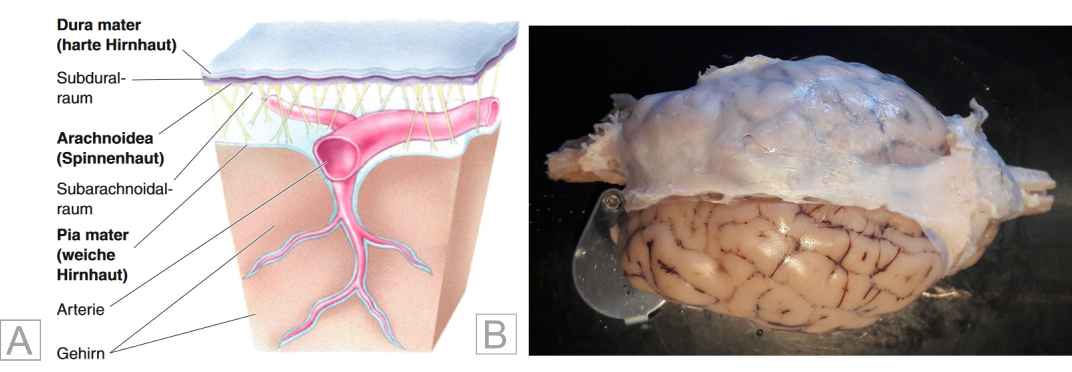
\includegraphics[width=\textwidth]{pictures/Bilder_Jule/Andere/hirnhaeute2.png}
	\caption[Die Hirnhäute]{\textbf{Die Hirnhäute.} \textbf{A}: Anordnung der drei Hirnhäute als Schema. \textbf{B}: Veranschaulichung der Hirnhäute am Schafhirn. Über der linken Hemisphäre ist die Dura mater zu sehen. Auf der linken Hemisphäre ist die Pia mater zu sehen. Die Dura mater Arachnoidea wurde von dieser Hälfte inklusive Arachnoidea entfernt.\\
	Abbildung~A aus \textit{Neurowissenschaften}, Bear et al. \textsuperscript{\cite[7]{neurowissenschaften_baer}}.}
	\label{fig:hirnhaeute}
\end{figure}


\subsubsection{Anhängende Strukturen}
\label{subsubsec:Hirnanhangsstrukturen}
%%%%%%%%%%%%%%%%%%%%%%%%%%%%%%%%%%%%%%%%%%%%%%%%%%%%%%%%%%%

\subsubsection*{Riechepithelium} \index{Riechepithel}
%%%%%%%%%%%%%%%%%%%%%%%%%%%%%%%%%%%%%%%%%%%%%%%%%%%%%%%%%%%%

Das Riechepithelium befindet sich außerhalb des Gehirns und ist am rostralen Ende mit diesem Verbunden. Es kleidet als Anteil der Nasenschleimhaut die obere Nasenmuschel und die gegenüberliegende Nasenscheidewand aus und überdeckt  ein  System aus Strömungskörpern (Abb.~\ref{fig:Riechepithel}). Das Riechepithel stellt die erste Station der Riechbahn dar. In diesem mehrschichtigen Sinnesepithel sind die chemorezeptiven Riechsinneszellen lokalisiert. Die axonalen Fortsätze dieser Zellen ziehen bis in die vordere Schädelgrube, wo sich der Bulbus olfactorius\index{Bulbus olfactorius} befindet. Bei Spezies mit gutem Riechvermögen nehmen Riechepithel und Bulbus olfactorius mehr Platz ein als bei Tieren, für deren Lebensweise der Riechsinn verhältnismäßig weniger relevant ist, wie beispielsweise bei Menschenaffen.

\begin{figure}[H]
    \centering
    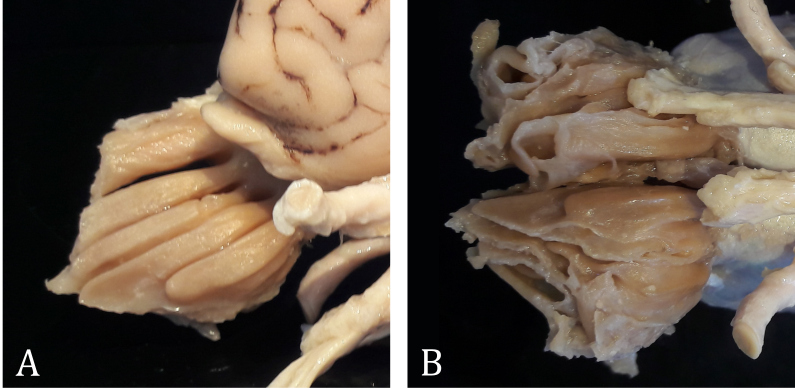
\includegraphics[width=0.8\textwidth]{pictures/Bilder_Jule/Schaf/Ausschnitte/Riechepithel.png}
    \caption[Riechepithelium Schaf]{\textbf{Riechepithelium Schaf}. Mediale (\textbf{A}) und inferiore (\textbf{B}) Ansicht des Riechepitheliums des Schafes.}
    \label{fig:Riechepithel}
\end{figure}{}


\subsubsection*{Hypophyse}
\label{subsubsec:hypophyse} \index{Hypophyse! allgemein}
%%%%%%%%%%%%%%%%%%%%%%%%%%%%%%%%%%%%%%%%%%%%%%%%%%%%%%%%%%%%

Die Hypophyse liegt inferior, leicht caudal des Chiamsa opticums und rostral des Mammillarkörpers. Über den Hypophysenstiel (Infundibulum) hängt sie am Hypothalamus (Abb.~\ref{fig:hypophyse}) \textsuperscript{\cite[4]{trepel2011neuroanatomie}}. Die Hypophyse besteht aus zwei Teilgebieten, der Neurohypophyse\index{Hypophyse! Neurohypophyse} und der Adenohypophyse\index{Hypophyse! Adenohypophyse}. Dabei ist lediglich die \textbf{Neurohypophyse} (Hypophysenhinterlappen) Teil des Diencephalons. Die Neurohypophyse besitzt keine dichte Blut-Hirn-Schranke. Dadurch können Hormone, die von den dort lokalisierten Nervenzellen sezerniert werden, via Neurosekretion ins Blut gelangen. Die deutlich größere \textbf{Adenohypophyse} (Hypophysenvorderlappen) umhüllt teilweise den kleineren Hypophysenhinterlappen. Sie ist kein Bestandteil des Gehirns, sie ist lediglich an das Diencephalon angelagert. Somit besteht die Adenohypophyse nicht aus Nervengewebe, sondern aus Drüsenepithel. Durch die dort gebildeten glandotropen Hormone kann die Adenohypophyse auf endokrine Drüsen, wie die Schilddrüse oder die Nebennierenrinde, wirken. Diese Drüsen nehmen dann durch die Produktion eigener Hormone  Einfluss auf periphere Organe. Auch Effektorhormone werden in der Adenohypophyse gebildet. Diese können direkt, ohne Zwischenschaltung weiterer Drüsen, auf periphere Organe wirken. Die Hormone der Adenohypophyse sind unter anderem an der Pigmentierung der Haut, an der Milchbildung in der Brustdrüse, am Körperwachstum und an der Reifung von Ei- und Spermienzellen beteiligt. Generell ist die Hypophyse als das hormonelle 'Ausführungsorgan' des Hypothalamus\index{Hypothalamus} (Kap.~\ref{subsubsec:Hypothalamus}) zu betrachten  \textsuperscript{\cite[8]{trepel2011neuroanatomie}}.

\begin{figure}[H]
    \centering
    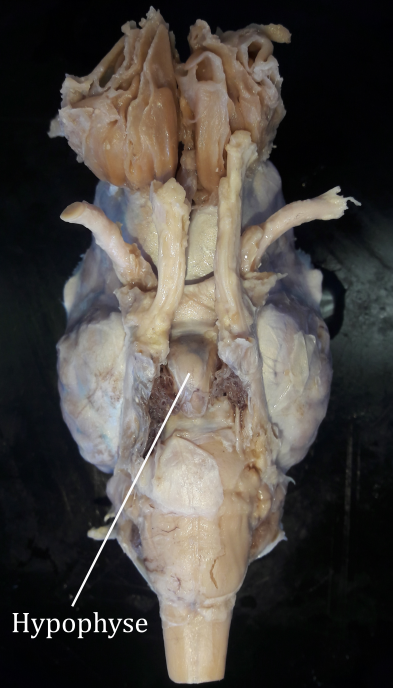
\includegraphics[width=0.5\textwidth]{pictures/Bilder_Jule/Schaf/Aussenansicht/Hypophyse.png}
    \caption[Hypophyse Schaf]{\textbf{Hypophyse Schaf}}
    \label{fig:hypophyse}
\end{figure}


%%%%%%%%%%%%%%%%%%%%%%%%%%%%%%%%%%%%%%%%%%%%%%%%%%%%%%%%%%%%%

%______________________Jacqui's Teil_________________________

%%%%%%%%%%%%%%%%%%%%%%%%%%%%%%%%%%%%%%%%%%%%%%%%%%%%%%%%%%%%%
% Allgemeine sensorische Bahnen
\newpage
\section{Allgemeine sensorische Bahnen} \label{sec:sensorische_Bahnen}
Dieses Kapitel behandelt die allgemeine Sensorik, \index{Sensorik! allgemein} die im Gegensatz zu speziellen Sensorik (Kapitel~ \ref{sec:spezsens}) steht. In der allgemeinen Sensorik sind die Sinne zusammen gefasst, welche über den ganzen Körper verteilt sind. Dazu gehören unter anderem die Somatosensorik\index{Sensorik! Somato-}, die Propriozeption\index{Propriozeption} und die Viszerosensorik \index{Sensorik! Viszero-} \textsuperscript{\cite[22]{kandel2013principles}}. Die spezielle Sensorik \index{Sensorik! speziell} fasst jene Sinne zusammen, welche auf Grund der Cephalisation bei Säugern nach vorne in den Kopf verlagert sind.
\\
\noindent
Die Somatosensorik zeichnet sich durch die Repräsentation der direkten äußeren Welt und der inneren Welt aus. Bei der Repräsentation der Außenwelt unterscheidet man bei Säugetieren zwischen zwei Rezeptorsystemen: Zum einen die haarlose Haut in den Handinnenflächen, an der Fußunterseite, an den Lippen und der Nase, zum anderen die behaarte Haut mit hoch spezialisierten Tastsinneszellen, innerviert durch die Bewegungen des Follikels auf den Blutsinus \index{Blutsinus} der Vibrissen \index{Sinushaar} \textsuperscript{\cite[24]{paxinos2014rat}}.
Die Propriozeption kodiert die Informationen der relativen Position der Extremitäten und anderer Körperteile im Raum und bildet in den Vorderextremitäten die Grundlage für abstrakte Wahrnehmung von Objektgrößen und Gewicht. Einen weiteren Bereich in der Somatosensorik bildet der Sinn, der Schmerzen und Temperatur verarbeitet \textsuperscript{\cite[24]{paxinos2014rat}}.
In den folgenden Kapiteln wird am Beispiel der Ratte näher auf die unterschiedlichen Systeme und deren Unterschiede eingegangen.


% Somatosensorik
\subsection{Somatosensorik \index{Sensorik! Somato-} des Körpers}
Die Somatosensorik des Körpers wird in zwei Systeme unterteilt, wobei der Tastsinn \index{Tastsinn} und die Propriozeption das lemniskale System \index{System! lemniskal} bilden und der Schmerz- und Temperatursinn das anterolaterales System. \index{System! anterolateral} Beide Systeme werden bei Säugern durch die Rezeptoren unter der haarlosen Haut innerviert.

\subsubsection{Tastsinn und Propriozeption (lemniskales System)} \label{subsubsec:tastsinn}

\subsubsection*{Rezeptoren}
Die Rezeptoren \index{Rezeptoren! somatosensorisch} des lemniskalen Systems werden anhand ihrer Lage unter der Haut und ihrer Adaptationseigenschaften unterteilt. Dadurch unterscheiden sie sich in den Modalitäten, die sie kodieren. Bei der Lage wird unterschieden zwischen direkt unter der Oberfläche oder tiefer im Gewebe liegenden Nervenendigungen, sowie schneller bzw. phasischer und langsamer bzw. phasisch-tonischer Adaptation dieser Nerven.\\
Direkt unter der Hautoberfläche liegen die Meissner- und die Merkel-Rezeptoren \index{Rezeptoren! Meissner}\index{Rezeptoren! Merkel}, welche für Bewegung und Druck, sowie in abstrakterem Sinne für Form, Textur und das Greifen nach Objekten kodieren.
\textsuperscript{\cite[24]{paxinos2014rat}}. Tiefer unter der Haut liegen die Pacini-Rezeptoren\index{Rezeptoren! Pacini}, welche schnell adaptierende Rezeptoren sind, die für Vibrationen kodieren. Zusammen mit den Meissner- und Merkelrezeptoren bilden sie den bewussten Tastsinn. Die Neurone der Rezeptoren sind dicke, myelinisierte A$\upalpha$ Nervenfasern mit einer Leitgeschwindigkeit von 72-120 m/s \textsuperscript{\cite[22]{kandel2013principles}}. Unbewusst werden von den langsamen, tief unter der Haut liegenden, Ruffini-Rezeptoren \index{Rezeptoren! Ruffini} Informationen über die Dehnung der Haut und der Muskeln und damit der Position der Gelenke und Extremitäten, weiter gegeben.
Die Nervenfasern der Propriozeption sind dicke, myelinisierte A$\upbeta$ Nerven, deren Durchmesser etwas geringer ist als der der A$\upalpha$ Neurone.
Die Nervenfasern eines Hautgebiets werden zu einem peripheren Nervenstrang gebündelt und ziehen in das Spinalganglion \index{Spinalganglion} innerhalb des Wirbelkanals. Die Zellkörper der Nervenfasern liegen in diesem Spinalganglion und sind umgeben von speziellen Gliazellen. Zwischen den Nervenzellen verlaufen fenstrierte Kapillaren, die die Nervenfasern mit den nötigen Nährstoffen versorgen. 

\subsubsection*{Rückenmark}
Die Axone der Nerven ziehen weiter in die Wirbelsäule. Da hier keine synaptische Verschaltung statt findet, ziehen die Axone direkt in die weiße Substanz des Rückenmarks und steigen parallel zum Verlauf der Wirbelsäule auf. Die Axone unterhalb des sechsten thorakalen Segments (T6) bilden den \textbf{Fasciculus gracilis} \index{Fasciculus! gracilis} und die Axone oberhalb des sechsten Thorakalsegments (T6) formen den \textbf{Fasciculus cuneatus} \index{Fasciculus! cueatus} im dorsalen Teil der weißen Substanz des Rückenmarks (Abb.~\ref{fig:bahnen_rueckenmark}) \textsuperscript{\cite[8]{paxinos2014rat}}. F.~gracilis und F.~cuneatus bilden somit die wichtigste aufsteigende Bahn für die sensorischen Informationen aus dem Tastsinn und der Eigenwahrnehmung hinauf in den Hirnstamm. 
Die Trennung zwischen F.~gracilis und F.~cuneatus ist wichtig, da sie in zwei anatomisch unterschiedlichen Kernen des Hirnstamms terminieren. Sie bilden zusammen mit anderen kleineren Bahnen den Hinterstrang (eng.: dorsal column) \textsuperscript{\cite[22]{kandel2013principles}}. 

\begin{figure}[H]
    \centering
    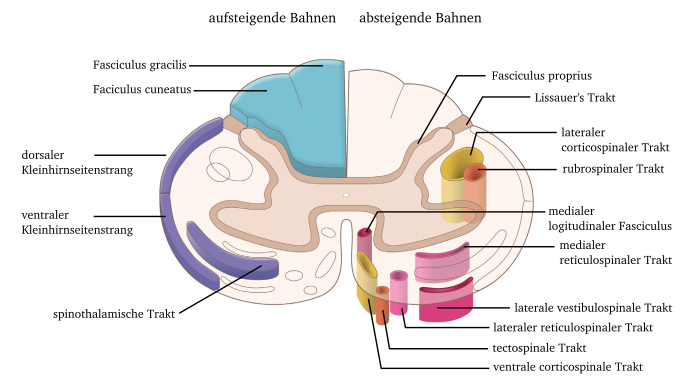
\includegraphics [width = \textwidth]
    {pictures/somatosensory/aufabsteigendeBahnen_Rueckenmark.png}
    \caption[Auf- und Absteigende Bahnen im Rückenmark]{\textbf{Auf- und Absteigende Bahnen im Rückenmark.} Zur besseren Veranschaulichung der Bahnen sind die Bahnen in der Abbildung nach absteigenden Bahnen auf der linken Seite und absteigenden Bahnen auf der rechten Seite aufgeteilt. Beide Gruppen kommen jeweils gespiegelt auch auf der anderen Seite vor. \\
    Abbildung aus \textit{Neuroanatomy}, Crossman und Neary
    \textsuperscript{\cite[8]{crossman2014neuroanatomy}}.}
    \label{fig:bahnen_rueckenmark}
\end{figure}

\subsubsection*{Nucleus gracilis und Nucleus cuneatus - Medulla}

Die Axone des \textbf{Fasciculus~gracilis} terminieren im \textbf{Nucleus~gracilis} \index{Nucleus! gracilis} in der Medulla. Auf gleicher Ebene der Medulla enden auch die Axone des \textbf{Fasciculus~cuneatus} im \textbf{Nucleus~cuneatus}\index{Nucleus! cuneatus}. Zusammen werden die beiden Kerne auch Hinterstrangkerne\index{Hinterstrangkerne} oder im englischen dorsal column nuclei genannt. In Abbildung~\ref{fig:nucleus_cuneatus} kann man den Nucleus~cuneatus (gelb) sehen. Der Nucleus liegt dorsal des Kerngebiets des Trigeminusnervs (Sp5I) und lateral des vierten Ventrikels (4V). Die Abbildung zeigt nicht den Nucleus gracilis.
\\
\noindent
Beide Nuclei sind zylindrisch geformt und in rostrocaudaler Richtung ausgedehnt. Die afferenten Neurone aus derselben Hautregion enden in der rostrocaudalen Ausdehnung auf einer Linie. Verschiedene Hautregionen werden lateral-medial repräsentiert. Die somatosensorische Repräsentation auf dieser Ebene gleicht einem auf dem Rücken liegenden, kopflosen Homunculus. Dabei liegen die distalen Körperregionen lateral und die proximalen Hautregionen medial in den Nuclei. Die taktilen und propriozeptiven Informationen des Kopfes (Kap.~\ref{sec:somatokopf}) werden in den angrenzenden \textit{Nucleus principalis nervi trigemini} \index{Nucleus! principalis, Pr5} repräsentiert \textsuperscript{\cite[22]{kandel2013principles}}. 

\begin{figure}[H]
    \centering
    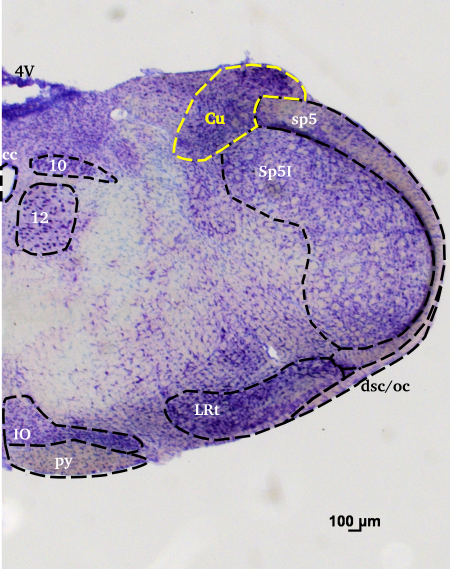
\includegraphics{pictures/somatosensory/nucleus_cuneatus.png}
    \caption[Lage des Nucleus cuneatus in der Medulla]{\textbf{Lage des \textit{Nucleus cuneatus} in der Medulla.} Nissl-Färbung der Rattenhirns auf der Höhe der Medulla (N02-3). Der Ausschnitt zeigt die rechte Seite vom Zentralkanal (cc) bis zum Trigeminusnerv (sp5). Oberhalb des Kerngebiets des Trigeminusnervs (SP5I) liegt der Nucleus~cuneatus (Cu). Die Schnittebene beinhaltet sowohl Teile der Medulla, daran zu erkennen, dass der vierter Ventrikel (4V) angeschnitten ist, als auch Teile des Rückenmarks, daran zu erkennen, dass der Zentralkanal (cc) zu sehen ist. Weitere Kerngebiete sind: der dorsale Kern des Nervus vagus (10), der Kern des Nervus hypoglossus (12), die untere Olive (IO) und der Nucleus reticularis lateralis (LRt). Ebenfalls zu sehen sind die Pyramidenbahn (py), der dorsaler spinocerebellarer Trakt/olivocerebraler Trakt (dsc/oc) und der Trigeminusnerv (sp5).}
    \label{fig:nucleus_cuneatus}
\end{figure}

\subsubsection*{Der Mediale Lemniscus}

\begin{figure}[H]
    \centering
    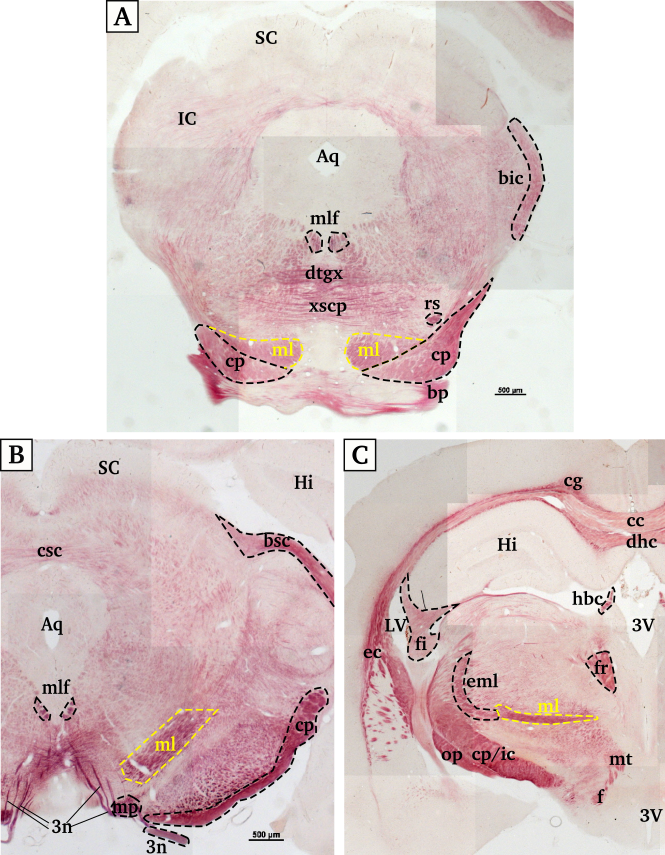
\includegraphics[width = 0.85\textwidth] {pictures/somatosensory/medial_lemniscus.png}
    \caption[Verlauf des medialen Lemniscus]{\small{\textbf{Verlauf des \textit{medialen Lemniscus.}} Faserschnitte auf der Höhe des Mesencephalons (A \& B) und des Diencephalons (C). Man kann den Verlauf des medialen Lemniscus in der Schnittserie über 3450~$\upmu$m verfolgen.\\
    \textbf{A:} (F14-4): Colliculus superior (SC), Colliculus inferior (IC), Aquädukt (Aq), Brachium des IC (bic), brachia pontis (bp, engl.: middle cerebellar peduncle), Großhirnstiele (Pedunculi cerebri) (cp), dorsale tegmentale Dekussation (dtgx), Fasciculus longitudinalis medialis (mlf), rubrospinaler Trakt (rs), Dekussation des SC Pedunkels (xscp).
    \textbf{B:} (F17-3): Nervus oculomotorius (3n), Hippocampus (Hi), Brachium des SC (bsc), Kommissur des SC (csc), Pedunculus mamillaris (mp).
    \textbf{C:} (F20-3): dritter Ventrikel (3V), lateraler Ventrikel (LV), zentrale Kommissur (cc), Cingulum (cg), dorsale Hippocampuskommissur (dhc), Capsula externa (ec), externe medulläre Lamina (eml), Fornix (f), Fimbria (fi), Fasciculus retroflexus (fr), Commissura habenularum (hbc), Capsula interna (ic), mammillothalamischer Trakct (mt), optischer Trakt (op)}}
    \label{fig:medialer_lemniscus}
\end{figure}

In den Hinterstrangkernen ist die erste synaptische Verbindung im lemniskalen System. Von den primär afferenten Axonen aus dem Rückenmark wird das Signal an die Nervenfasern des \textbf{medialen~Lemniscus} \index{Lemniscus! medial} weiter geleitet. Diese kreuzen die Mittellinie auf der Höhe der Medulla und verlaufen anschließend contralateral \textsuperscript{\cite[22]{kandel2013principles}}. 
Der \textbf{mediale~Lemniscus} liegt ventral-medial in der Medulla und zieht von der Medulla bis in den Thalamus des Diencephalons. Die Veränderung der Lage des medialen~Lemniscus \index{Lemniscus! medial} kann man in Abbildung~\ref{fig:medialer_lemniscus} verfolgen. Er beginnt bereits auf der Höhe des Nucleus cuneatus (Abb.~\ref{fig:somato_pathway}) und zieht sich dann ventral-medial unterhalb des Aquädukts (Abb.~\ref{fig:medialer_lemniscus}~A) weiter in rostraler Richtung. Dabei verändert er seine Lage in sofern, dass er von ventral-medial nach medial-lateral (Abb.~\ref{fig:medialer_lemniscus}~B) zieht. Der mediale~Lemniscus zieht auf der Höhe des dritten Ventrikels (Abb.~\ref{fig:medialer_lemniscus}~C) zentral im Diencephalon bis in den Thalamus.

\subsubsection*{Thalamus im lemniskalen System}
\index{Thalamus! lemniskales System}
Die Informationen aus den Hautschichten von den Meissner-, Merkel- und Pacini-Rezep-toren, die über die primär afferenten Neurone und den medialen Lemniscus kommen, werden im lateralen und medialen \textbf{Nucleus ventralis posterior} (eng.: lateral and medial
ventral posterior nuclei) \index{Nucleus! ventralis posterior} verarbeitet. Propriozeptive Informationen aus den Gelenken und dem Bauchraum werden über den medialen Lemniscus an den oberen Nucleus ventralis posterior (eng.: superior ventral posterior nucleus) weitergeleitet \textsuperscript{\cite[22]{kandel2013principles}}. 
In der Nisslfärbung des Rattenhirns ist keine Abgrenzung der einzelnen Nuclei des Thalamus sichtbar. Der Thalamus, als Verschaltungszentrale des Diencephalons, liegt bei der Ratte zentral unter dem dritten Ventrikel (3V, Abb.~\ref{fig:thalamus_somato}) und oberhalb des Hypothalamus. 
Am Beispiel des Menschen werden in Kapitel \label{subsubsec:thalamus} die einzelnen Kerne im Thalamus gezeigt, wobei die Lage der somatosensorischen Kerne gut in Abbildung \ref{fig:thalamus_nuclei}~A~\&~B zu sehen ist.
Die zweite synaptische Verschaltung im Thalamus gibt die Informationen an die Neurone der thalamisch-cortikalen Verbindung weiter, welche die Informationen dann an den primären somatosensorischen Cortex leitet.

\begin{figure}[H]
    \centering
    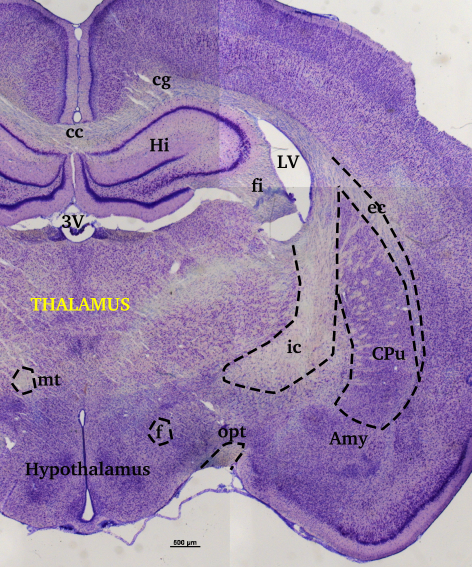
\includegraphics[width = 0.8\textwidth]
    {pictures/somatosensory/thalamus_somato.png}
    \caption[Thalamus im lemniskalen System]{\textbf{Thalamus im lemniskalen System.} Rechte Gehirnhälfte (N23-3) der Ratte auf der Höhe des Thalamus und des dritten Ventrikels (3V). Auf derselben Höhe sind als prominente Hirnstrukturen der Hippocampus (Hi), der Hypothalamus und die zentrale Kommissur (Corpus callosum, cc) zu sehen. Weitere Strukturen sind Cortex, Amygdala (Amy), Caudate Putamen (CPu), Cingulum (cg), äußere Kapsel (ec), Fornix (f), Fimbria (fi), innere Kapsel (ic), lateraler Ventrikel (LV), mammillothalamischer Trakt (mt), optische Bahn (opt).}
    \label{fig:thalamus_somato}
\end{figure}

\subsubsection*{Primärer Somatosensorischer Cortex}
\label{subsubsec:S1}
Der \textbf{somatosensorische Cortex} \index{Cortex! primär somatosensorisch} liegt beim Menschen auf dem postzentralen Gyrus,\index{Gyrus! postzentral} direkt hinter dem \textit{Sulcus centralis}. Der primäre somatosensorische Cortex (S1) setzt sich aus den Brodmann-Arealen 3a, 3b, 1 und 2 zusammen und endet anterior im Sulcus centralis, wo er an den primären Motorcortex (Brodmann-Areal~4) angrenzt. Posterior des S1 liegt der posteriore Parietallappen mit den Brodmann-Arealen 5 und 7. In Abbildung~\ref{fig:S1_Cortex} ist ein horizontaler Schnitt durch die verschiedenen Areale des primären somatosensorischen Cortex und den angrenzenden Strukturen zu sehen \textsuperscript{\cite[23]{kandel2013principles}}. 

\begin{figure}[H]
    \centering
    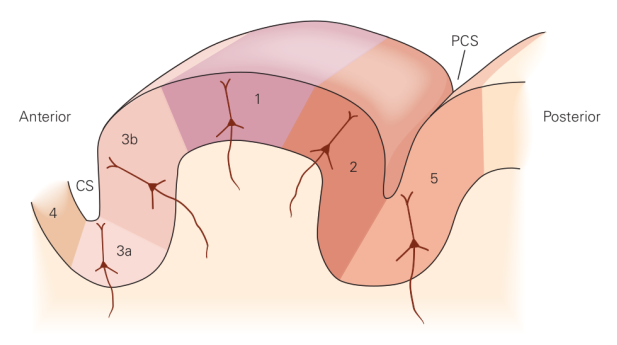
\includegraphics{pictures/somatosensory/S1_Cortex.png}
    \caption[Primärer somatosensorischer Cortex]{\textbf{Primärer somatosensorischer Cortex (S1).} Der primäre somatosensorische Cortex (S1) setzt sich aus den Brodmann-Arealen 3a, 3b, 1 und 2 zusammen und endet anterior im Sulcus centralis (CS). Dort grenzt er an den primären Motorcortex (Brodmann-Areal 4). Posterior des S1 liegt der posteriore Parietalcortex mit den Brodmann-Arealen 5 und 7. Er grenzt sich vom postzentralen Gyrus durch den postzentralen Sulcus (PCS) ab. Abbildung aus \textit{Principles of Neural Systems}, Kandel et al. \textsuperscript{\cite[23]{kandel2013principles}}.}
    \label{fig:S1_Cortex}
\end{figure}

Betrachtet man den somatosensorischen Cortex in seiner Ausdehnung entlang des Sulcus centralis \index{Sulcus! centralis}, wie auch die Schnittebene in Abbildung~\ref{fig:somato_pathway} verläuft, wird nochmal die Somatotopie \index{Somatotopie} deutlich. Hierbei ist vor allem der Unterschied zwischen den Tieren sehr prominent. Die somatosensorischen Informationen auf der Hautoberfläche unterscheiden sich in der Größe der rezeptiven Felder und in der daraus resultierenden Relevanz. Auf Grund dessen werden einige Körperregionen mehr repräsentiert als andere. Eine Darstellung dieser Überrepräsentation ist der Homunculus (Abb.~\ref{fig:somato_homunculus}). Der Homunculus \index{Homunculus} der Ratte ähnelt dem des Hasen.


\begin{figure}[H]
    \centering
    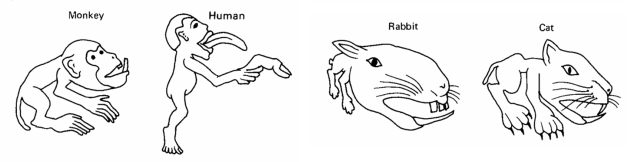
\includegraphics[width = \textwidth] {pictures/somatosensory/homunculus.png}
    \caption[Homunculus]{\textbf{Homunculus.} Homunculi des Affen, Menschen, Hasen und der Katze. Abbildung aus der Vorlesung \textit{Integrative Neurobiology: Somatosensory System}, J. Ostwald \textsuperscript{\cite{Ostwald}}.}
    \label{fig:somato_homunculus}
\end{figure}

\newpage
Areal~3b erhält Informationen aus den bewussten Mechanorezeptoren der Haut. In diesem Cortexareal werden vor allem die Wahrnehmung der taktilen Reize und deren Form und Textur verarbeitet, wohingegen in Areal~3a die Wahrnehmung aus der Körperhaltung und der Propriozeption verarbeitet wird. Areal~1 und 2 erhalten ihre Informationen aus Areal~3b. In Areal~1 werden die Informationen aus der strukturellen Beschaffenheit des Objekts weiterverarbeitet, in Areal~2 Informationen über die Größe und Gestalt. Alle vier Areale des primären somatosensorischen Cortex projizieren in den sekundären somatosensorischen Cortex (S2) \textsuperscript{\cite[12]{neurowissenschaften_baer}}.
\\
\noindent Der sekundäre somatosensorische Cortex \index{Cortex! sekundär somatosensorisch} liegt unterhalb des primären somatosensorischen Cortex und ist für die Verarbeitung der Informationen aus beiden S1 zuständig. Über den Corpus callosum erhält er Informationen aus der jeweils anderen Großhirnhemispäre. Er verarbeitet die bilateralen rezeptiven Felder und ist für den Lerntransfer zwischen den beiden Hemispären zuständig. Der S2 ist auch für die generelle Aufmerksamkeit bezüglich taktiler Informationen verantwortlich \textsuperscript{\cite[12]{neurowissenschaften_baer}}.

Im Gegensatz zu der Lage des somatosensorischen Cortex beim Menschen steht die Lage bei der Ratte. Da Ratten ein lisencephales Gehirn besitzen und bei diesen Tieren kein Sulcus centralis ausgebildet ist, ist die Lokalisation des Areals nicht anhand dessen zu bestimmen. Anhand der Schichtung und Färbungen wurde der somatosensorische Cortex bei der Ratte identifiziert (Abb.~\ref{fig:S1_Cortex_Ratte}). Die Neurone in dem Teil des Cortex (anteriore parietale Region) wurden durch eine stark ausgeprägte granuläre Schicht IV und der stärksten Myelinisierung aller Cortexareale identifiziert. \textsuperscript{\cite[22]{paxinos2014rat}}
\\
\begin{figure}[H]
    \centering
    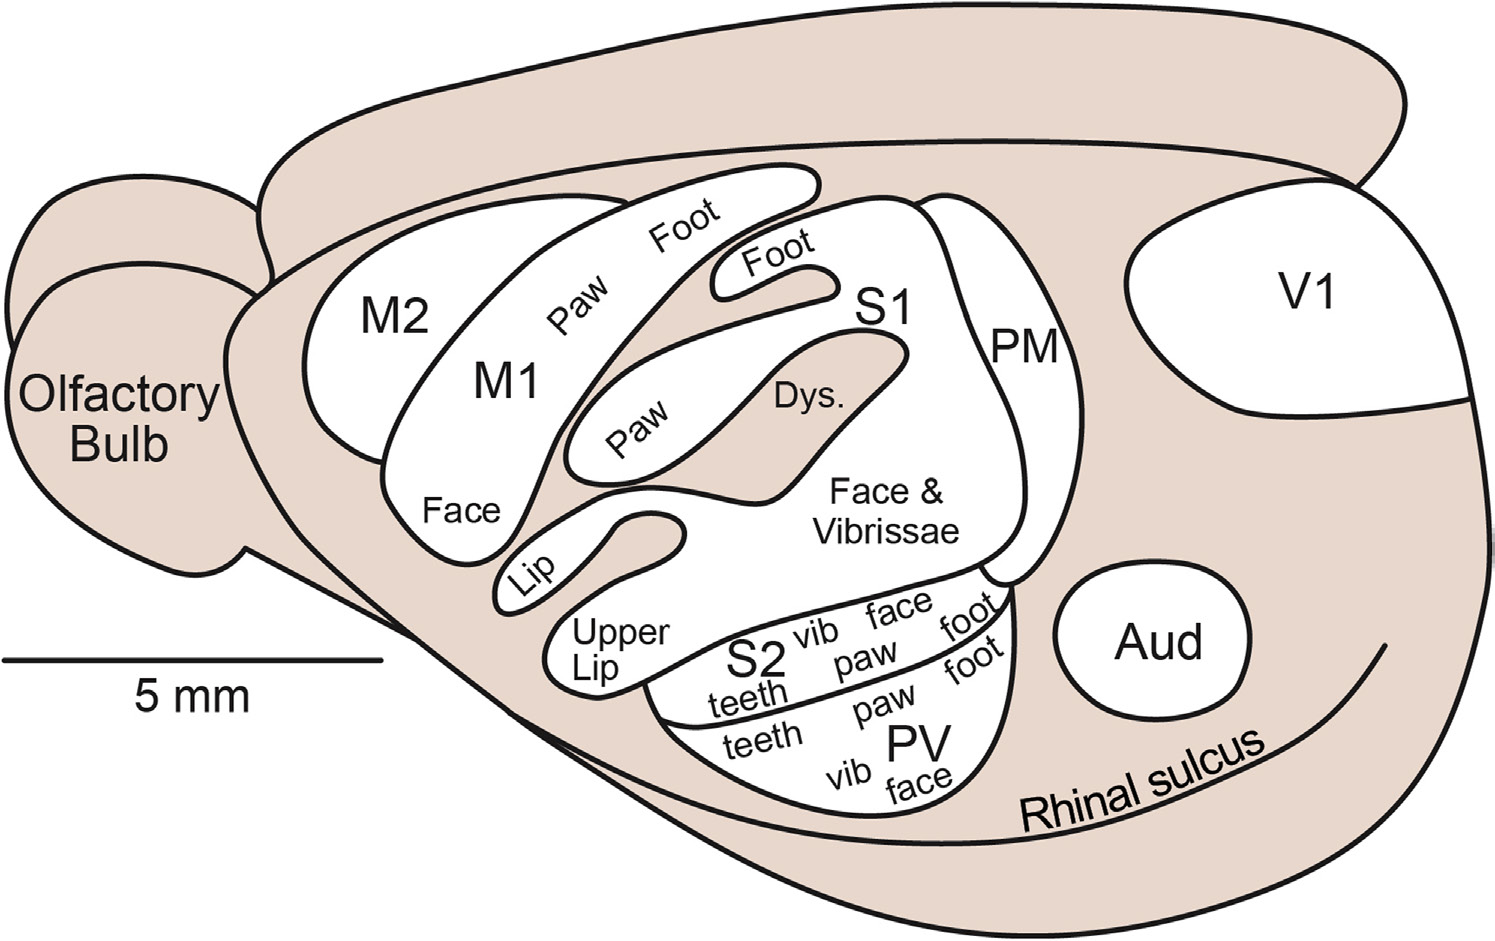
\includegraphics[width = 0.8\textwidth] {pictures/somatosensory/Somato_cortex_ratte.png}
    \caption[Somatosensorischer Cortex der Ratte]{\textbf{Somatosensorischer Cortex der Ratte.} Primärer (S1) und sekundärer (S2) somatosensorischer Cortex mit der Repräsentation der einzelnen Körperregionen. Außerdem ist die \textit{Fissura rhinalis} (Rhinal sulcus) gezeigt, welche den Neocortex vom Archicortex trennt. Anterior vom somatosensorischen Cortex ist der Motorcortex mit primärem (M1) und sekundärem (M2) Motorcortex. Ventral des S2 liegt das parietale ventrale somatosensorische Areal (PV) und posterior das posteriore mediale Areal (PM). Als Reverenz sind noch der auditorische Cortex (Aud) und der visuelle Cortex (V1) gezeigt. Abbildung aus \textit{The Rat Nervous System}, Paxinos et al. \textsuperscript{\cite[24]{paxinos2014rat}}.}
    \label{fig:S1_Cortex_Ratte}
\end{figure}

\subsubsection*{Somatosensorische Bahnen}

\begin{figure}[H]
    \centering
    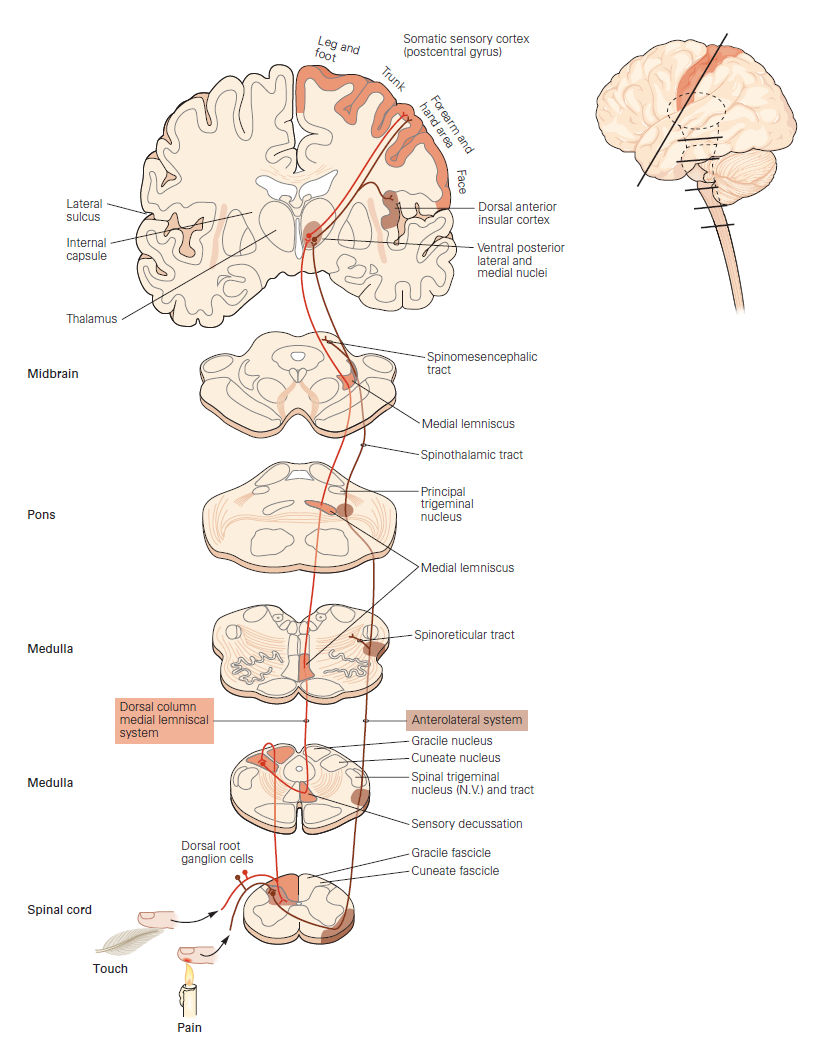
\includegraphics{pictures/somatosensory/pathway_somatosensory2.png}
    \caption[Aufsteigende Bahnen der Somatosensorik]{\textbf{Aufsteigende Bahnen der Somatosensorik.} Die aufsteigenden Bahnen der Somatosensorik sind getrennt in das lemniskale (rot) und das anterolaterale (braun) System. Beginnend im Rückenmark bis hin zum primären somatosensorischen Cortex posterior vom \textit{Sulcus centralis}. Die Bahnen sind am Beispiel des Menschen schematisch dargestellt und sind auf den Ebenen des Rückenmarks, der Medulla, der Pons, des Mittelhirns und des Cortex zu verfolgen.\\
    Abbildung aus \textit{Principles of Neural Science}, Kandel et al. \textsuperscript{\cite[22]{kandel2013principles}}.}
    \label{fig:somato_pathway}
\end{figure}

\newpage    
\subsubsection{Schmerz und Temperatursinn (anterolaterales System)}
\label{subsubsec:Schmerzsinn}
\index{System! anterolateral}
Der Schmerz- und Temperatursinn \index{Schmerzsinn} \index{Temperatursinn} hat vor allem eine schützende Funktion auf unseren Körper. Er wird unter dem Begriff der Nozizeption (lat.: 'nocere' für Schaden) zusammengefasst. Er warnt uns vor Verletzungen oder zu großer Hitze, worauf wir dann reflexartig reagieren und zurückweichen oder die Verletzung behandeln können. Die Schmerzwahrnehmung geht von den somatosensorischen Strukturen in der Haut aus und wird von dort zu den höheren Gehirnarealen weitergeleitet.

\subsubsection*{Rückenmark}

Die meisten der Nozizeptoren \index{Nozizeptoren} sind einfache Nervenendigungen primärer sensorischer Faser und können generell in drei Gruppen eingeteilt werden, die thermischen, mechanischen und polymodalen Nozizeptoren \textsuperscript{\cite[24]{kandel2013principles}}. Auch die Zellkörper der Nozizeptoren des Körpers liegen im dorsalen Wurzelganglion und terminieren im Hinterhorn des jeweiligen Segments. Ihre Synapsen konzentrieren sich in den Schichten I, IV, V, VII, und X des Hinterhorns (Abb.~\ref{fig:graymatter}) \textsuperscript{\cite[25]{paxinos2014rat}}.

\begin{figure}[H]
        \centering
        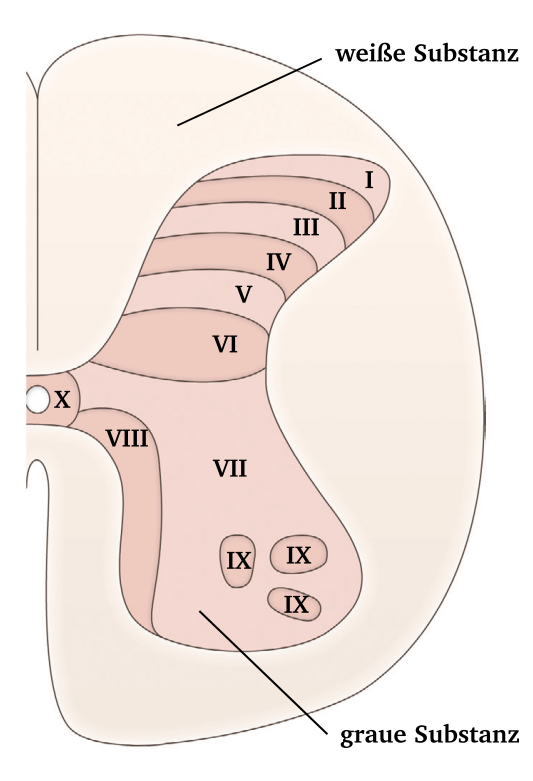
\includegraphics[width = 0.5\textwidth]
        {pictures/somatosensory/gray_matter.png}
        \caption[Schichten in der grauen Substanz des Rückenmarks]{\textbf{Schichten in der grauen Substanz des Rückenmarks.} Die Abbildung zeigt schematisch die rechte Seite des Rückenmarks mit weißer und grauer Substanz. Die Schichten der grauen Substanz beginnen im Hinterhorn mit Schicht I und gehen bis Schicht VIII im Vorderhirn. Die Schicht XI liegt in Schicht VIII. Schicht X umgibt den Zentralkanal. Abbildung nach \textit{Neuroanatomy}, Crossman und Neary
        \textsuperscript{\cite[8]{crossman2014neuroanatomy}}.}
        \label{fig:graymatter}
    \end{figure}

\newpage
Diese Synapsen verbindet die Nozizeptoren mit den spinothalamischen Neuronen. Wie der Name dieser Neurone bereits sagt, ziehen sie vom Rückenmark bis in den Thalamus. Die Zellkörper der Neurone liegen in der grauen Substanz des Rückenmarks, während die Axone in der weißen Substanz des Rückenmarks parallel zum Verlauf der Wirbelsäule in Bahnen auf- und absteigen. Die Axone der spinothalamischen Nervenzellen kreuzen auf der Ebene der ersten Synapse die Mittellinie und steigen in der contralateralen weißen Substanz zum lateralen Bereich des Thalamus auf. Bei Ratten bildet die größte Gruppe der spinothalamischen Neurone, jene, welche auf der Höhe der Halswirbelsäule der grauen Substanz beginnen \textsuperscript{\cite[25]{paxinos2014rat}}.


\subsubsection*{Thalamus im anterolateralen System}
\index{Thalamus! anterolaterales System}
Die aufsteigende spinothalamische Bahn \index{Tractus! spinothalamisch} im Rückenmark ist anhand ihrer Verbindung von Rückenmark und Thalamus benannt und verläuft ventral des Vorderhorns \index{Vorderhorn} (Abb.~\ref{fig:bahnen_rueckenmark}). Auch diese Neurone sind somatotopisch organisiert. Die Axone aus Schicht I steigen im lateralen Funiculus,\index{Funiculus! lateral} auf, wohingegen die Axone aus den Schichten IV, V und X in der ventralen weißen Substanz aufsteigen und in den medialen und intralaminaren Thalamus projizieren \textsuperscript{\cite[25]{paxinos2014rat}}. 
Mehrere Nuclei des Thalamus verarbeiten die Informationen aus dem anterolateralen Sytem. Die wichtigsten zwei Gebiete sind die lateralen und die medialen Kerngebiete. 
Die lateralen Kerngebiete bestehen aus dem ventro-posterior medialen Nucleus, dem ventro-posterior lateralen Nucleus und dem posterioren Nucleus. Sie erhalten Informationen über Nozizeption-spezifische Neurone mit breitem dynamischen Spektrum. Dieses Kerngebiet beschäftigt sich deshalb unter anderem mit der präzisen Lokalisation von Verletzungen und der Übertragung dieser Informationen als bewussten Schmerz \textsuperscript{\cite[24]{kandel2013principles}}.
\\
\noindent Die medialen Kerngebiete des Thalamus setzen sich aus dem zentral-lateralen Nucleus und dem intralaminaren Komplex zusammen. Sie bekommen unter anderem Input aus dem spinothalamischen Trakt, aber auch aus der \textbf{Formatio reticularis}.\index{Formatio reticularis} Neurone im medialen Thalamus reagieren auf schädigende Stimuli und projizieren in die Basalganglia und den Cortex \textsuperscript{\cite[24]{kandel2013principles}}.

\subsubsection*{Cortex}
\index{Cortex! somatosensorisch}
Bei \textbf{Ratten} wurden Reaktionen auf einen schädigenden Stimulus im primären somatosensorischen Cortex festgestellt. Demnach werden hier zum Teil die Informationen aus dem anterolateralen System verarbeitet. Die Neurone aus dem nozizeptiven System befinden sich in der Schicht V und VI des somatosensorischen Cortex, wohingegen sich die mechanorezeptiven Neurone in Schicht II~-~V befinden. Die rezeptiven Felder des Schmerz- und Temperatursinns im Cortex sind im Vergleich zu den der mechanosensorischen rezeptiven Felder größer und zudem meist inhibitorisch \textsuperscript{\cite[25]{paxinos2014rat}}.
\\
\noindent Im Gegensatz dazu steht die Verarbeitung der Schmerz- und  Temperaturwahrnehmung beim \textbf{Menschen}. Einige der Neurone im \textit{Gyrus cinguli},\index{Gyrus! cinguli} oberhalb des \textit{Corpus callosum},\index{Corpus! callosum} und der Inselrinde (\textit{Cortex insularis}),\index{Insula} innerhalb des Sulcus lateralis, reagieren stark und ausschließlich auf Reize aus dem nozizeptiven somatosensorischen System. Der Gyrus cinguli ist wie schon in Kapitel \ref{subsubsec:Grosshirnrinde} und \ref{subsec:limisches_system}) beschrieben, ein Teil des limbischen Systems. Es wird vermutet, dass das limbische System bei der Verarbeitung von Gefühlszuständen, assoziiert mit der Schmerzwahrmnehmung, beteiligt ist. Neurone des Thalamus projizieren direkt zur Inselrinde (Insula)\index{Insula}, vor allem aus dem medialen und venteroposterior-medialen Nucleus des Thalamus. Die Inselrinde verarbeitet hauptsächlich Informationen über den Zustand innerhalb des Körpers und wirkt bei der autonomen Reaktion des Körpers auf den Schmerz mit \textsuperscript{\cite[24]{kandel2013principles}}.

\subsubsection*{Spinomesencephalischer Trakt und  Spinoreticularer Trakt}

Sowohl der spinomesencephalische Trakt\index{Tractus! spinomesencephal}, als auch der spinoreticuläre Trakt\index{Tractus! spinoreticulär} sind Abzweigungen vom spinothalamischen Trakt. Es ist bekannt, dass der spinoreticuläre Trakt bei der absteigenden Schmerzunempfindlichkeit und bei autonomen Regulationen eine Rolle spielt. Der spinomesencephalische Trakt ist an der Schmerzwahrnehmung beteiligt. Dabei ist er für den motivational-affectiven Aspekt, also für die Vermeidung von Schmerz, weil er unangenehm ist, zuständig. Aus diesem Grund ist der spinomesencephalische Trakt auch beim Auslösen von Aktivität im absteigenden Kontrollsystem involviert \textsuperscript{\cite[24]{kandel2013principles}}.


\newpage
\subsection{Somatosensorik des Kopfes (trigeminales System) \index{System! trigeminal}}
\label{sec:somatokopf}
Die Somatosensorik des Kopfes beinhaltet beim Menschen die Informationen aus den somatosensorischen Rezeptoren von Gesicht und Mund. Bei einigen Säugetieren kommen noch wichtige Informationen aus den Vibrissen im Gesichtsbereich, die sogenannte \textbf{Viszerosensorik} \index{Viszerosensorik}, hinzu. Die Verarbeitung dieser Informationen über das trigeminale System wird im Folgenden beschrieben. Auf die Rolle der Vibrissen wird genauer eingegangen.

\subsubsection*{Vibrissen}
Die Aufgabe von Vibrissen\index{Vibrissa} ist die Nahorientierung und -erkundung, weshalb sie an verhaltensrelevanten Körperteilen vorkommen. Die meisten Säuger, die ihre Nahrung mit der Schnauze ergreifen und nicht mit den Händen, besitzen Vibrissen im Kopfbereich um die Schnauze. Aber auch an anderen Körperstellen, wie z.B. unter dem Kinn (Wüstenspring-mäuse) oder zwischen den Zehen (Katzen), gibt es diese Tasthaare. Die Vibrissen sind lange, steife Tasthaare, welche von einem Blutsinus umgeben sind. Die Schnurrbarthaare \index{Schnurrbarthaare|see{Vibrissa}} sind spezialisierte Vibrissen, die zusätzlich noch bewegt werden können. 
Die Auslenkung der Vibrissen führt zu einer Aktivierung der freien Nervenendigungen, die im Haarschaft zwischen Haar und Blutsinus liegen \textsuperscript{\cite[5]{heldmaier2003tierphysiologie}}.

\subsubsection*{Nucleus des Trigeminus}

Die freien Nervenendigungen der Vibrissen und die Mechanorezeptoren im Gesicht und Mund bilden gemeinsam den fünften Hirnnerv (\textit{Nervus trigeminus})\index{Hirnnerven! 05. N. trigeminus}. Die Ganglien der Nerven liegen alle außerhalb des Hirnstamm im \textit{Ganglion Gasseri} (eng.: trigeminal ganglion)\index{Ganglion Gasseri}, wobei eine Großzahl der Neurone die Vibrissen repräsentiert.
\\
\noindent
Der Trigeminus ist der fünfte Hirnnerv (CN~V). Je nach Lage in den Schnitten durch das Gehirn ist die Bezeichnung des Trigeminus unterschiedlich. Auf der Höhe der Medulla ist es noch der spinale Trakt des Trigeminus (sp5, Abb.~\ref{fig:somato_Pr5}), wohin gegen auf der Höhe des Aquädukts im Mesencephalon von dem sensorischen Trigeminus \index{Trigeminus} (s5, Abb.~\ref{fig:somato_Pr5}) die Rede ist. Der Trigeminus ist auch in sich geordnet, wobei die Neurone aus dem Tastsinn vorne im Trigeminus repräsentiert sind und die Neurone aus dem Schmerzsinn hinten.
\\
\noindent
Die Axone des Ganglion Gasseri ziehen auf der Höhe des Pons in den Hirnstamm und teilen sich dort, um in den Nucleus principalis des Trigeminus (Pr5, \textit{Nucleus principalis nervi trigemini}) \index{Nucleus! principalis, Pr5} und die drei Gebiete des spinalen Nucleus des Trigeminus (Sp5, \textit{Nucleus spinalis nervi trigemini}) \index{Nucleus! spinalis, Sp5}, oralis (Sp5O), interpolaris (Sp5I) und caudalis (Sp5C) zu ziehen. Alle Gebiete gehören zum \textit{Nucleus trigemini}, welcher sich über das Mesencephalon, den Pons und die Medulla erstreckt \textsuperscript{\cite[5]{heldmaier2003tierphysiologie}}. 
Hinzu kommen Informationen aus dem Nervus facialis (CN~VII),\index{Hirnnerven! 07. N. facialis} dem Nervus glossopharyngeus \index{Hirnnerven! 09. N. glossopharyngeus} (CN~IX) und dem Nervus vagus (CN~X), welche die Hautbereiche um die Ohren, sowie die Nasen und Rachenregion abdecken
\textsuperscript{\cite[12]{neurowissenschaften_baer}}.
\\
\noindent Die Neurone des Nucleus principalis reagieren auf Reize aus dem Kopfbereich, der Zunge und des Gesichts. Zusammen mit dem Nucleus gracilis und Nucleus cuneatus repräsentieren die drei Nuclei den sensorischen Input des gesamten Körpers. Die Neurone im Nucleus principalis (Pr5, Abb.~\ref{fig:somato_Pr5}), und in Teilen auch die des Nucleus spinalis (Sp5, Abb.~\ref{fig:somato_Pr5}), bekommen die Information aus spezifischen Körperregionen und sind durch Neuropil in Cluster geteilt. Die Cluster, die aus den einzelnen Vibrissa gebildet werden sind, in der richtigen Schnittebene, gut zu sehen. Sie werden nach dem Zusammenhang mit den 'Barrels' im Cortex, im Nucleus principalis 'barrelettes' genannt \textsuperscript{\cite[5]{heldmaier2003tierphysiologie}}.

\begin{figure}[H]
    \centering
    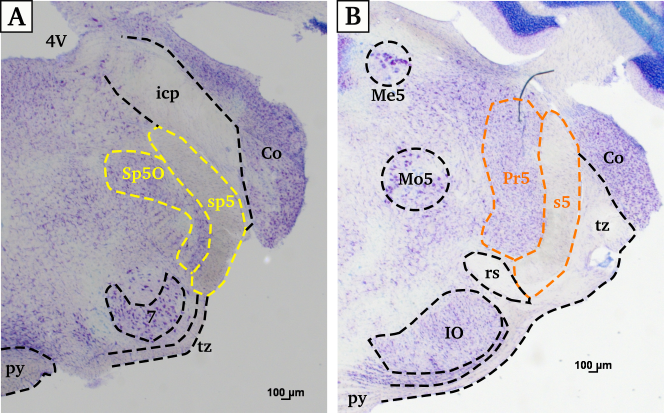
\includegraphics[width = \textwidth]
    {pictures/somatosensory/somato_kopf.png}
    \caption[Nucleus spinalis und Nucleus principalis des Trigeminus]{\textbf{Nucleus spinalis und Nucleus principalis des Trigeminus.}\\
     \textbf{A:}~(N06-4): Der Nucleus spinalis oralis (Sp5O) liegt in der Medulla, lateral auf der Höhe des Nucleus cochlearis (Co) und doral des Nucleus facialis (7). Des weiteren sieht man den spinalen Trigeminus (sp5) lateral dieses Nucleus. Weitere Strukturen sind der vierte Ventrikel (4V), das inferiore cerebellare Pedunkel (icp), die Pyramidenbahn (py) und der Trapezkörper (tz).
     \textbf{B:} (N09-3): Der Nucleus principalis (Pr5) des Trigeminus liegt im Mesencephalon lateral-dorsal auf Höhe der inferioren Olive (IO). Die Axone zum diesem Nucleus liegen im Trigeminus (s5). Weitere Strukturen sind der Nucleus cochlearis (Co), der Nucleus mesencephalicus des Trigeminus (Me5), der Nucleus motorius des Trigeminus (Mo5),  die Pyramidenbahn (py), der rubrospinale Trakt (rs) und der Trapezkörper (tz).}
    \label{fig:somato_Pr5}
\end{figure}

\subsubsection*{Nucleus mesencephalicus des Trigeminus}
Einige der Neurone, die für die somatosensorische Reizweiterleitung aus dem Kopfbereich zuständig sind, haben ihre Zellkörper nicht im Ganglion Gasseri. Dazu gehören die Neurone, die aus den Muskelspindeln kommen, sowie einige Neurone aus den Vibrissen und die Neurone der Zahnwurzeln. Die Zellkörper diese Neurone sind im Nucleus mesencephalicus des Trigeminus (Me5, Abb.~\ref{fig:somato_Pr5}) \index{Nucleus! mesencephalicus, Me5}lokalisiert. Die Axone dieser Neurone projizieren in den dorsomedialen Bereich des Nucleus principalis \index{Nucleus! principalis, Pr5} \textsuperscript{\cite[5]{heldmaier2003tierphysiologie}}.

\subsubsection*{Thalamus und Cortex}
Die Axone aus dem Nucleus principalis kreuzen die Mittellinie, stoßen zum medialen Lemniscus hinzu und ziehen in den Thalamus. Die Axone aus dem trigeminalen System ziehen in den medialen Part des Thalamus. Im Thalamus wird über synaptische Verschaltung die Information an die Nervenzellen der thalamocortikalen Verbindung zum primären somatosensorischen Cortex (S1) \index{Cortex! primär somatosensorisch}weiter gegeben. 
Wie schon in Kapitel \ref{subsubsec:S1} beschrieben, ist S1 für die Verarbeitung der somatosensorischen Reize aus dem Körper verantwortlich. Bei Ratten kommen die meisten somatosensorischen Informationen aus den Vibrissen. Von jeder Vibrisse gehen etwa 100 myelinisierte Nervenfasern ab. Über den Trigeminus werden die Informationen zuerst in den Nucleus principalis geleiten. Von dort aus ziehen andere Neurone weiter in den Thalamus und von dort in den Cortex. Die Neurone enden im Cortex \index{Barrel-Cortex} \index{Cortex! Barrel-Cortex} in abgegrenzten Strukturen, den sogenannten 'Barrel' (Abb.~\ref{fig:barrelcortex}~B). Die Anzahl der 'Barrels' entsprechen den der Vibrissen und die 'Barrels' sind nach ihrem Aufbau benannt ('barrels', engl. für Tonnen ): In der Nissl-Färbung (Abbildung~\ref{fig:barrelcortex}~C) sieht man die Neurone dicht gepackt um weniger dichte Bereiche. Die Wände der Tonnen bestehen aus dicht gepackten Neuronen, das Innere aus weniger dicht gepackten Bereichen \textsuperscript{\cite[8]{smith2008biology}}. 

\begin{figure}[H]
    \centering
    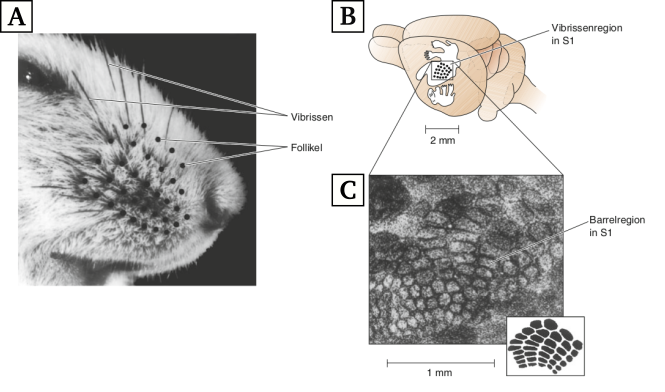
\includegraphics[width = \textwidth] {pictures/somatosensory/barrelcortex.png}
    \caption[Barrelcortex]{\textbf{Barrelcortex.} \textbf{A:} Die Lage der Vibrissen am Beispiel einer Maus. \textbf{B:} schematische Darstellung des primären somatosensorischen Cortex (S1) mit der Lage der 'Barrel' (engl. für Tonne, nach dem Aussehen der einzelnen cortikalen Areale jeder Vibrisse) in S1. Die 'Barrel' sind analog zur Lage der Vibrissen zueinander angeordnet. \textbf{C:} Barrelregion innerhalb von S1. Der Schnitt durch die 'Barrel' ist horizontal zum Cortex angelegt und mit Hilfe einer Nissl-Färbung angefärbt. Die Abbildung unten rechts zeigt erneut die Anordnung der Barrel in fünf Reihen, wie auch in \textbf{A} zusehen ist. \\
    Abbildung aus Aronoff und Petersen, 2008 \textsuperscript{\cite{barrelcortex2008}}.}
    \label{fig:barrelcortex}
\end{figure}

%%%%%%%%%%%%%%%%%%%%%%%%%%%%%%%%%%%%%%%%%%%%%%%%%%%%%%%%%%%%%%
%%%%%%%%%%%%%%%%%%%%%%%%%%%%%%%%%%%%%%%%%%%%%%%%%%%%%%%%%%%%%%

\newpage
\section{Spezielle sensorische Bahnen}
% verweis auf dieses Kapitel mit \ref{sec:spezsens}
\label{sec:spezsens}
Die speziellen sensorischen Bahnen umfassen unter anderem die Hörbahn \index{Hörbahn} und die Sehbahn\index{Sehbahn}, mit denen sich hauptsächlich dieses Kapitel beschäftigen wird. Es gibt weitere, spezialisierte Sinne, wie zum Beispiel den elektrischen Sinn bei Fischen, die beiden chemischen Sinne für Geruch und Geschmack und der Magnetsinn bei Zugvögeln \textsuperscript{\cite{smith2008biology}}. Diese werden nicht in dieser Zusammenfassung behandelt, spielen aber bei anderen Tierarten eine tragende Rolle und sollten aus diesem Grund hier kurz erwähnt werden.

\subsection{Hörbahn}

Das auditorische System \index{System! auditorisch} ist für die Verarbeitung von Schallwellen, die über die Luft oder Wasser übertragen und vom System empfangen werden, zuständig. Vibrationen, die über den Untergrund oder festes Substrat übertragen werden und mechanisch wahrgenommen werden, gehören zum Vibrationssinn, der eng mit dem auditorischen Sinn verwandt ist.
Dabei hat der auditorische Sinn zwei Aufgaben: Zum einen die Detektion des Schalls und zum anderen die Lokalisation der Schallwelle. Das Richtungshören ist jedoch nicht für alle Tiere möglich. Zudem ist es auch bei jenen Tieren, die dazu befähigt sind, nicht im gesamten Hörbereich gleich ausgelegt \textsuperscript{\cite[18]{penzlin2005tierphys}}.

\subsubsection*{Spiralganglion}
\index{Spiralganglion}
Die Funktion unserer Ohren ist die Energie eines akustischen Signals von der Außenwelt einzufangen und von einem mechanischen Signal in ein elektrisches umzuwandeln. Diese Umwandlung findet an den inneren Haarsinneszellen in der Cochlea statt. Dort wird durch die Auslenkung der Haarbündel an den inneren Haarsinneszellen (eng.: inner hair cell, IHC) \index{Haarsinneszellen! innere, IHC} die Zelle depolarisiert oder hyperpolarisiert, je nach Auslenkungsrichtung \textsuperscript{\cite[30]{kandel2013principles}}. Die Depolarisation der Haarzellen führt zur Öffnung spannungsgesteuerter Kalziumkanäle und dem damit verbundenen Einstrom von \ce{Ca^2+}. Durch den Einstrom des \ce{Ca^2+} wird der Neurotransmitter (wahrscheinlich Glutamat) freigesetzt und aktiviert die Spiralganglionzellen. Spiralganglionzellen sind bipolare Zellen, welche ihren Namen der spiralförmigen Struktur der Cochlea (Schneckenspindel) \index{Cochlea} verdanken, der sie folgen \textsuperscript{\cite[11]{neurowissenschaften_baer}}. Sie formen einen Teil des achten Hirnnervs (CN~VIII), der auch Nervus vestibulocochlearis \index{Hirnnerven! 08. N. vestibulocochlearis} genannt wird. Ungefähr 30~000 Ganglionzellen im Hörnerv werden durch die inneren Haarzellen innerviert. Das macht ungefähr 90\% des Nervs aus \textsuperscript{\cite[30]{kandel2013principles}}. 
Innere Haarzellen haben keinen efferenten Eingang von höheren Hirnstrukturen. Anhand der Neuronenverteilung in der afferente Bahn wird die funktionale Bedeutung zwischen den inneren und äußeren Haarzellen deutlich. Die afferenten Fasern, ausgehend von den IHC, sind myelinisiert (Typ I) und bilden 95\% der afferenten Fasern, während 5\% der Fasern, afferente unmyelinsierte Typ~II Fasern, von den äußeren Haarzellen ausgehen. Bei den inneren Haarzellen gibt dabei die Regel, dass jedes Axon nur von einer Haarzelle innerviert wird, eine Haarzelle innerviert jedoch im Durchschnitt zehn Fasern.  \textsuperscript{\cite[30]{kandel2013principles}}.   
\\
\noindent Die afferenten Nervenfasern der IHC kodieren die Stimulusfrequenz und dessen Intensität. Aufgrund der Beschaffenheit der Basilarmembran \index{Basilarmembran} der Cochlea, werden die Frequenzen tonotopisch von hohen Frequenzen am ovalen Fenster bis zu tiefen Tönen am Helicotrema \index{Helicotrema} entlang der Basilarmembran aufgeteilt \textsuperscript{\cite[22]{paxinos2014rat}}. Infolge ihrer Größe und Funktion sind die Type I Fasern, ausgehend von den inneren Haarzellen, sehr viel besser verstanden. Die Bahnen, die die Informationen aus diesen Fasern führen, werden im Folgenden als einzige thematisiert.

\begin{figure}[H]
    \centering
    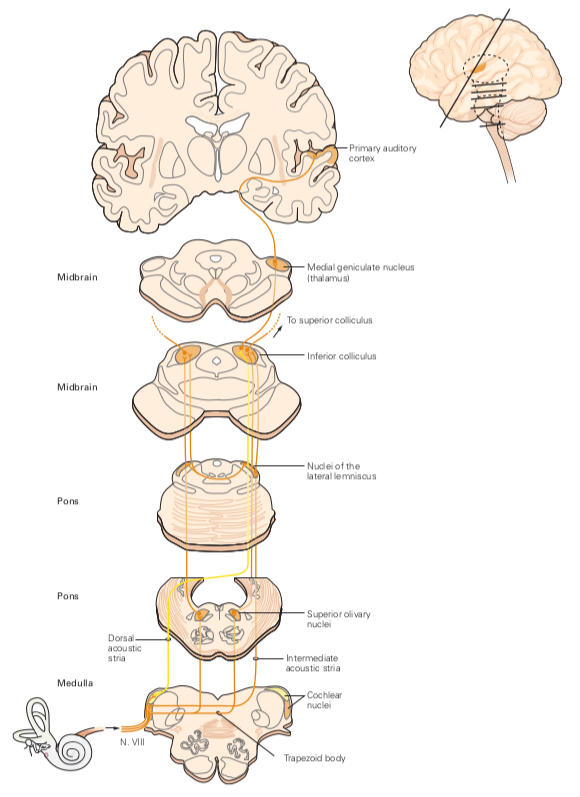
\includegraphics{pictures/auditory/hoerbahn_pathway.png}
    \caption[Hörbahn]{\textbf{Hörbahn.} Die einzelnen Stationen der Hörbahn des Menschen von den Spiralganglionzellen in der Cochlea bis zum primären auditorischen Cortex anhand skizzierter Gehirnschnitte. Abbildung nach \textit{Principles of Neural Science}, Kandel et al. \textsuperscript{\cite[30]{kandel2013principles}}.}
    \label{fig:hoerbahn_pathway}
\end{figure}

\newpage
\noindent Efferente Fasern im Hörnerv innervieren die äußeren Haarzellen \index{Haarsinneszellen! äußere, OHC} in der Cochlea, deren Aufgabe darin besteht die mechanische Auslenkung der Basilarmembran und der damit verbundenen Tektorialmembran \index{Tektorialmembran} zu verstärken oder zu unterdrücken. Infolgedessen kommt es zu einer verstärkten Selektivität und Sensibilität der Frequenzwahrnehmung \textsuperscript{\cite[22]{paxinos2014rat}}.

\subsubsection*{Nucleus cochlearis}

Die afferenten Ganglionzellen aus dem Hörnerv ziehen auf der Höhe der Medulla in den Hirnstamm und dort in das Kerngebiet des \textit{Nucleus cochlearis} (CN). \index{Nucleus! cochlearis} Dieser befindet sich  lateral auf Höhe der Medulla (Abb.~\ref{fig:hoerbahn_pathway}) und bekommt nur Input aus dem Hörnerv der ipsilateralen Seite. Der CN besteht aus dem dorsalen Nucleus cochlearis (DCN) und dem ventralen Nucleus cochlearis (VCN), welcher wiederum in den anteroventralen (AVCN) und den posteroventralen (PVCN) Nucleus unterteilt wird \textsuperscript{\cite[22]{paxinos2014rat}}. Bei Ratten liegt der ventrale Nucleus cochlearis mediolateral flach an der Medulla, während der dorsale Nucleus cochlearis sich um den unteren Kleinhirnstiel (engl.: restiform body) \textsuperscript{\cite[22]{paxinos2014rat}} zieht.
\\ \noindent Die auditorischen Nervenfasern verzweigen sich im Nucleus cochlearis in die verschiedenen Teile des CNs (Abb.~\ref{fig:Nucleus_cochlearis}~B). Jede Faser gabelt sich in einen aufsteigen Ast zum AVCN und einen absteigenden Ast zum PVCN und DCN und leitet die Informationen an verschiedene Neurone dieser Teilbereiche weiter \textsuperscript{\cite[22]{paxinos2014rat}}. Die Neurone im ventralen Nucleus cochlearis kodieren für verschiedene Eigenschaften, je nach Zelltyp. Im Allgemeinen schärfen sie das Timing und die Informationen aus dem Klangspektrum. 
\\

\begin{figure}[H]
    \centering
    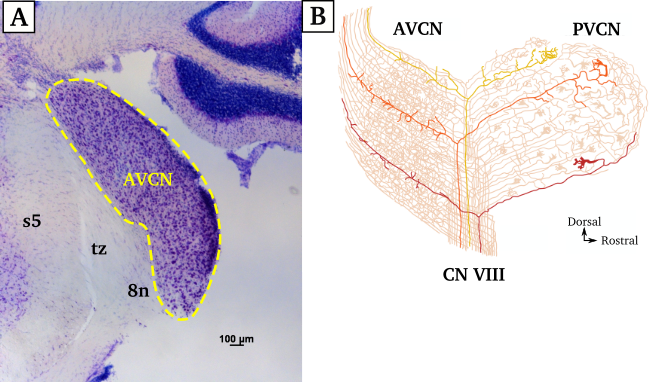
\includegraphics[width = \textwidth]{pictures/auditory/CN.png}
    \caption[Nucleus cochlearis]{\textbf{Nucleus cochlearis.} \textbf{A:} Nissl-Färbung (N09-1) der rechten Seite der Medulla. Es sind der anteroventrale Nucleus cochlearis (AVCN), der Trigeminus (s5), der Trapezkörper (tz) und der achte Hirnnerv (8n, Hörnerv) zu sehen. \textbf{B:} Verlauf der Nervenfasern aus dem achten Hirnnerv (CN VIII, 8n) im ventralen Nucleus cochlearis. Sowohl im anteroventralen (AVCN) als auch im posteroventralen (PVCN) Bereich des CNs werden die Fasern nach der Frequenz tonotopisch geordnet, von den tiefen Frequenzen (rot) ventral bis zu den hohen Frequenzen (gelb) im dorsalen Bereich. \\
    Abbildung B nach \textit{Principles of Neural Science}, Kandel et al. \textsuperscript{\cite[31]{kandel2013principles}}, abgeändert.}
    \label{fig:Nucleus_cochlearis}
\end{figure}

\newpage
Eine wesentliche Rolle spielt die zeitliche Abfolge der Töne bei der Weiterverarbeitung der Informationen in der oberen Olive, wohingegen die Verarbeitung des Klangspektrums in den ipsilateralen DCN, die ipsilaterale laterale obere Olive (LSO), den contralateralen ventralen Nucleus des lateralen Lemniscus und den contraleteralen Colliculus inferior projiziert wird \textsuperscript{\cite[31]{kandel2013principles}}. 
\\\\
\noindent Der dorsale Nucleus cochlearis bekommt einerseits direkten Input von den Neuronen aus dem Hörnerv, zum anderen indirekten Input aus dem ventralen CN. Der dorsale CN integriert akustische und somatosensorische Informationen um die Richtung der Schallquelle zu bestimmen \textsuperscript{\cite[31]{kandel2013principles}}. 


\subsubsection*{Obere Olive}
\index{Olive! obere Olive}
Ein Großteil der Nervenzellen aus dem Nucleus cochlearis projizieren in die obere Olive. Die \textbf{obere Olive} (\textit{Nucleus olivaris superior}) ist für die Verarbeitung auditorischer Informationen wichtig und umfasst mehrere Kerngebiete. Innerhalb der Säugetiere variieren diese Kerngebiete. Drei Kerngebiete können bei fast allen Spezies gefunden werden: Die \textbf{laterale obere Olive} (engl.: lateral superior olive, \textbf{LSO}), die \textbf{mediale obere Olive} (engl.: medial superior olive, \textbf{MSO}) und der \textbf{mediale Nucleus des Trapezkörpers} (engl.: medial nucleus of the trapezoid body, \textbf{MNTB}). Die LSO ist ein S-förmiges Kerngebiet im lateralen Bereich der oberen Olive. Sie ist durch ihre markante Struktur leicht zu erkennen (Abb.~\ref{fig:obere_Olive}). Die MSO liegt medial der LSO und ist bei Ratten ein deutlich kleineres Kerngebiet als beim Menschen. Der mediale Nucleus des Trapezkörpers (MNTB) befindet sich lateral in der oberen Olive \textsuperscript{\cite[29]{paxinos2014rat}}.

In Nagetieren, wie der Ratte, gibt es ein viertes, ausgeprägtes Kerngebiet, den \textbf{oberen paraoliven Nucleus} (engl.: superior paraolivary nucleus, \textbf{SPO}). Dieses Kerngebiet befindet sich im dorsomedialen Bereich der oberen Olive. Es bekommt Informationen aus dem contralateralen Nucleus cochlearis und projiziert in den Colliculus inferior auf der ipsilateralen Seite \textsuperscript{\cite[29]{paxinos2014rat}}. Die SPO entschlüsselt besonders gut Muster in Tönen, sowie Informationen in zeitlichen Mustern. Das spielt in der Wahrnehmung von Kommunikation eine wichtige Rolle, im Besonderen bei akustischen Schwebungen in Vokalisationen bei Tieren und Sprachsignalen beim Menschen \textsuperscript{\cite[29]{paxinos2014rat}}. 
\\

\noindent Die drei Hauptkerne der oberen Olive spielen eine wichtige Rolle in der Verarbeitung von Schall. Aufgrund der Beschaffenheit der Cochlea werden dort nur die einzelnen Frequenzen kodiert. Es werden keine Informationen über die Richtung der Schallquelle kodiert. Das Richtungshören wird in der oberen Olive, durch die Verarbeitung der Informationen aus beiden Ohren, integriert. Sie ist damit die erste Schaltstelle in der Hörbahn, die Input sowohl von der ipsilateralen, als auch von der contralateralen Seite, aus den jeweiligen Nuclei cochlearis, bekommt.
\\

\index{Olive! obere Olive! MSO}
\noindent Die \textbf{mediale obere Olive} (\textbf{MSO}) ist tonotopisch arrangiert. Die tiefen Töne werden dorsal in der MSO verarbeitet, wohingegen hohe Frequenzen im ventralen Part verarbeitet werden. Der Anteil der tiefen Töne ist in der MSO proportional über repräsentiert. Aus diesem Grund ist die sie in der Ratte (Abb.~\ref{fig:obere_Olive}) klein, da Ratten im hochfrequenten Bereich hören.

Die mediale obere Olive erhält exzitatorischen Input aus den beiden Nuclei, wobei die lateralen Dendriten der MSO, die Informationen aus dem ipsilateralen Nucleus cochlearis erhalten und die medialen Dendriten aus dem contralateralen Nucleus \textsuperscript{\cite[29]{paxinos2014rat}}. Da die Neurone aus den Nuclei nur zu einer bestimmt Phase des Tons feuern (engl.: \textbf{phase-locking}), kann mit Hilfe der interauralen Zeitdifferenz und dem 'coincidence detection model' die Richtung, aus der der Ton kam, bestimmt werden \textsuperscript{\cite[31]{kandel2013principles}}. Da der interaurale Abstand bei Ratten sehr klein ist, ist die Zeitdifferenz zwischen den Ohren ebenfalls sehr klein. Er lässt sich nur für sehr tiefe Töne berechnen.

Die Axone der MSO projizieren in den \textbf{dorsalen Nucleus des lateralen Lemniscus} (\textbf{DLL}) und in den \textbf{Colliculus inferior} (\textbf{IC}) \textsuperscript{\cite[29]{paxinos2014rat}}.
\\

\begin{figure}[H]
    \centering
    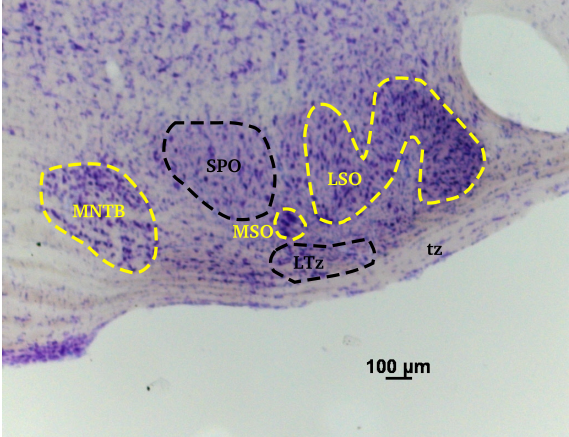
\includegraphics{pictures/auditory/obere_olive.png}
    \caption[Obere Olive]{\textbf{Obere Olive.} Nissl-Färbung (N10-1) der oberen Olive des Pons. Mit den drei Hauptkernen: Der mediale obere Olive (MSO), der lateralen oberen Olive (LSO) und dem medialen Nucleus des Trapezkörpers (MNTB), sowie dem für Nager speziellen oberen paraoliven Nucleus (SPO). Des Weiteren liegen in der oberen Olive das Kerngebiet des lateralen Nucleus des Trapezkörpers (LTz) und der Trapezkörper (tz) selbst. Letzterer verbindet die oberen Oliven beider Hemisphären miteinander und befindet sich ventral des Komplex der oberen Olive.}
    \label{fig:obere_Olive}
\end{figure}

Die \textbf{laterale obere Olive} (\textbf{LSO}) und der \textbf{mediale Nucleus des Trapezkörpers} (\textbf{MNTB}) \index{Nucleus! MNTB} bilden gemeinsam eine Einheit, welche über die Berechnung der interauralen Intensitätsdifferenz das Richtungshören bei hohen Tönen ermöglicht. 
Die tonotopische Anordnung der LSO zieht sich entlang der S-Form von hohen Tönen (medial) bis zu tieferen Tönen (lateral). Die LSO der Ratte ist im Vergleich zum Menschen deutlich größer. Das hängt unter anderem mit der Überrepresentation der hohen Töne in der lateralen oberen Olive und dem Hörbereich von Ratten zusammen.

Die LSO erhält bilateralen Input. Der ventrale Nucleus cochlearis (VCN) der ipsilateralen Seite leitet die Informationen exzitatorisch an die LSO weiter. Vom contralateralen VCN werden die Informationen exzitatorisch an den MNTB, der jeweils anderen Seite, über den Trapezkörper weiter gegeben. Von dort aus wird das Signal inhibitorisch an die LSO derselben Seite weiter geleitet.
Somit bekommen die Neurone der LSO indirekten inhibitorischen Input aus dem contralateralen Nucleus cochlearis und exzitatorischen Input aus dem ipsilateralen Nucleus cochlearis.

Die laterale obere Olive projiziert bilateral in den zentralen Nucleus des Colliculus inferior (\textbf{IC})\index{Colliculus! inferior}. Dabei wird auf die ipsilaterale Seite inhibitorisch, auf die contralaterale Seite exzitatorisch projiziert.
Des Weiteren projiziert ein Teil der Neurone auch in den dorsalen Nucleus des lateralen Lemniscus (\textbf{DLL}) \textsuperscript{\cite[29]{paxinos2014rat}}.


\subsubsection*{Lateraler Lemniscus}
\index{Lemniscus! lateral}
Die afferenten Nervenfasern aus der oberen Olive bilden den \textbf{Lemniscus lateralis} (\textbf{ll}), welcher über das Tegmentum pontis in den \textbf{Colliculus inferior} (\textbf{IC}) \index{Colliculus! inferior} zieht und dort terminiert (Abb.~\ref{fig:lateraler_lemniscus}). Einige der Axone aus der oberen Olive terminieren in den \textbf{Nuclei des lateralen Lemniscus}. Des Weiteren enden hier auch Nervenfasern, die direkt aus den Nuclei cochlearis kommen \textsuperscript{\cite[10]{crossman2014neuroanatomy}}. 
Die Nuclei des lateralen Lemniscus unterteilen sich in den \textbf{dorsalen Nucleus des lateralen Lemniscus} (\textbf{DLL}) \index{Nucleus! dorsaler Nucleus des lateralen Lemniscus} und den \textbf{ventralen Nucleus des lateralen Lemniscus} (\textbf{VLL}). \index{Nucleus! ventraler Nucleus des lateralen Lemniscus} Diese Unterteilung erfolgt anhand zweier funktional unterschiedlichen Systeme: die monoaurale Verarbeitung ventral und die binaurale Verarbeitung dorsal \textsuperscript{\cite[29]{paxinos2014rat}}. 
\\

Afferente Neurone ziehen aus dem contralateralen ventralen Nucleus cochlearis (VCN) und dem ipsilateralen MNTB in den \textbf{ventralen Nucleus des lateralen Lemniscus} (\textbf{VLL}). Der VLL ist vorwiegend für die Verarbeitung von präzisen zeitlichen Informationen zuständig.
Es wird vermutet, dass die Zwischenstation in dem ventralen Nucleus als Relaisstation auf dem Weg zum Colliculus inferior fungiert.
Der Nucleus ist aus isofrequenten Lamina aufgebaut und liegt im Pons (Abb.~\ref{fig:lateraler_lemniscus}). Die Afferenzen zum Colliculus inferior sind ebenfalls tonotopisch arrangiert. Sie terminieren im zentralen Bereich des IC \textsuperscript{\cite[29]{paxinos2014rat}}.
\\

Der \textbf{dorsale Nucleus des lateralen Lemniscus} (\textbf{DLL}) liegt oberhalb des ventralen Nucleus des lateralen Lemniscus im Pons (Abb.~\ref{fig:lateraler_lemniscus}). Er bekommt bilateralen Input. Diesen bekommt er von der contralateralen Seite aus dem ventralen Nucleus cochlearis (VCN) und dem DLL. Von der ipsilateralen Seite projizieren afferente Nervenfasern aus der MSO, SPO und dem VLL in den DLL. Zudem ziehen aus beiden Seiten Afferenzen aus der lateralen oberen Olive (LSO) in den DLL.
Aufgrund der vielen Verbindungen zu tiefer liegenden Kernen, wie der LSO und MSO, spielt der dorsale Nucleus eine wichtige Rolle beim Richtungshören. Läsionen im DLL bewirken ein Defizit im Richtungshören und eine Ungenauigkeit in der räumlichen Hörschärfe. 
Der DLL projiziert über den lateralen Lemniscus in beide Colliculi inferiores (IC) und über die Probst Kommissur in den gegenüberliegenden dorsalen Nucleus des lateralen Lemniscus
\textsuperscript{\cite[29]{paxinos2014rat}}.

\begin{figure}[H]
    \centering
    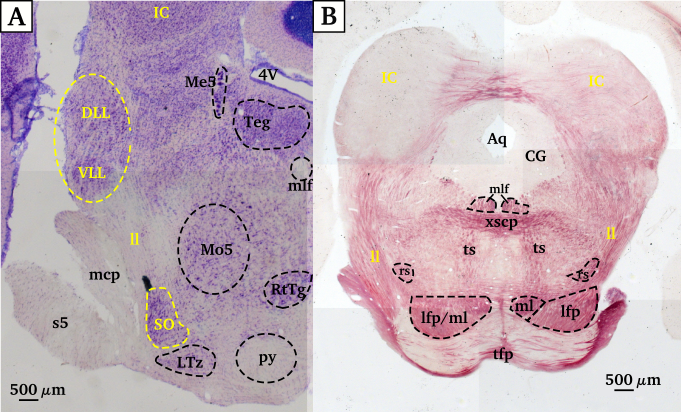
\includegraphics[width = \textwidth]{pictures/auditory/lateral_lemniscus.png}
    \caption[Der Lateraler Lemniscus und seine Kerne]{\textbf{Der Lateraler Lemniscus und seine Kerne.} Verlauf des lateralen Lemniscus und die Lage seiner Kerne in der Nissl-Färbung (N11-4) und der Faser-Färbung (F13-4). Die Schnittebenen sind 1200~$\upmu$m auseinander.\\
    \textbf{A:} Nissl-Färbung (N11-4) auf der Höhe des Pons, erkennbar am vierten Ventrikel (4V).
    Der laterale Lemniscus verbindet die obere Olive (SO) mit dem Colliculus inferior (IC). Einige der Verbindungen sind über den dorsalen (DLL) oder den ventralen (VLL) Nucleus des lateralen Lemniscus zwischen geschaltet. 
    Des Weiteren sind der Trigeminus (s5) und der Nucleus des mesencephalischen Trakts des Trigeminus (Me5) aus der Somatosensorik, sowie der motorische Nucleus des Trigeminus (Mo5) aus der Motorik zu sehen. 
    Weitere Kerngebiete und Fasertrakte sind: lateraler Nucleus des Trapezkörpers (LTz), mittleres cerebellare Pendunkel (mcp), medialer Fasciculus longitudinalis (mlf), Pyramidenbahn (py), reticulotegmentaler Nucleus des Pons (RtTg), Tegmentum (Teg).\\
    \textbf{B:} Verlauf des lateralen Lemniscus (ll) bis in den Colliculus inferior (IC) im Mesencephalon. Das zentrale Höhlengrau (CG) und das Aquädukt (Aq) sind zwei prominente Strukturen, die im Mesencephalon liegen. Des Weiteren sind folgende Fasertrakte zu sehen: Fasciculus longitudinalis des Pons (lfp), medialer Lemniscus (ml), medialer Fasciculus longitudinalis (mlf), rubrospinaler Trakt (rs), transversale Fasern des Pons (tfp), tectospinaler Trakt (ts), Kreuzung (Dekussation) des oberen cerebellaren Pedunkels (xscp).}
    \label{fig:lateraler_lemniscus}
\end{figure}

\newpage
\subsubsection*{Colliculus inferior und Corpus geniculatum mediale}

Die Fasern des lateralen Lemniscus ziehen in den \textbf{Colliculus inferior} (\textbf{IC}) \index{Colliculus! inferior} und terminieren dort. Der IC liegt bei der Ratte sichtbar im dorsalen Bereich des Mittelhirns, caudal vom Colliculus superior, mit dem er gemeinsam die Vierhügelplatte bildet (Kap.~\ref{subsubsec:Tectum}) \textsuperscript{\cite[29]{paxinos2014rat}}. 
Der IC integriert nahezu die gesamt Information aus den tiefer liegenden auditorischen Kerngebieten des Hirnstamms. Das macht ihn zu einem großen Integrationszentrum für die Verarbeitung des Richtungshörens, sowie für Tonhöhen \textsuperscript{\cite[29]{paxinos2014rat}}.

\begin{figure}[H]
    \centering
    \includegraphics{pictures/auditory/MG.png}
    \caption[Corpus geniculatum mediale]{\textbf{Corpus geniculatum mediale.} Das Corpus geniculatum mediale (MGN) liegt im Mesencephalon lateral-ventral des Colliculus superior (SC). Das Aquädukt (Aq) wird vom zentralen Höhlengrau (CG) umgeben und unterhalb liegt der Nucleus ruber (R), welcher sich ebenfalls im Mesencephalon befindet. Der Cortex liegt um das Mesencephalon herum. Dazu zählen der amygdaloid-hippocampale Bereich (AHi) der Cortex entorhinalis (Ent), Forceps major des Corpus callosum (fmj) und der Hippocampus (Hi). Nissl-Färbung (N16-3)}
    \label{fig:MG}
\end{figure}

Vom Colliculus inferior aus zieht die Hörbahn in den \textbf{medialen Kniehöcker} (\textit{Corpus geniculatum mediale}). \index{Corpus! geniculatum mediale} Der mediale Kniehöcker (\textbf{MGN}) liegt auf der posterolateralen Seite des Thalamus (Abb.~\ref{fig:MG}). Er ist eine runde Erhebung lateral-ventral des Colliculus superior. Der MGN ist das letzte Integrationszentrum in der auditorischen Hörbahn vor dem Cortex. Er bekommt Input aus dem Colliculus inferior (IC) über das \textit{Brachium colliculi inferioris}. Zudem terminieren absteigende Fasern aus dem auditorischen Cortex und dem reticularen Nucleus im MGN. Afferente Nervenfasern aus dem medialen Kniehöcker ziehen ipsilateral in den auditorischen Cortex \textsuperscript{\cite[29]{paxinos2014rat}}. Der mediale Kniehöcker ist in drei Untereinheiten aufgeteilt: den ventralen, den dorsalen und den medialen Part. Der ventrale mediale Kniehöcker hat eine rein akustische Funktion, wohingegen der dorsale Part bei akustischer Aufmerksamkeit mitwirkt und der mediale Part bei multisensorischer Erregung und emotionalem akustischen Lernen eine Rolle spielt \textsuperscript{\cite[29]{paxinos2014rat}}. 
\\
Eine weitere Bahn führt vom Colliculus inferior direkt in den Colliculus superior (SC), welcher bei reflexiven Bewegungen zur Orientierung eine Rolle spielt. Deswegen wird angenommen, dass im SC eine auditorische Karte der Umgebung erstellt wird. Ein Beispiel dafür sind Eulen, bei denen man solche drei-dimensionalen Karten gefunden hat. Zusammen mit Karten aus dem visuellen System und dem somatosensorischen System spielt der Colliculus superior \index{Colliculus! superior}eine entscheidende Rolle in der motorischen Orientierung während dem Greifen nach Gegenständen \textsuperscript{\cite[31]{kandel2013principles}}.


\subsubsection*{Primärer auditorischer Cortex}
\index{Cortex! primär auditorisch}

Die Fasern aus dem medialen Kniehöcker enden in einer tonotopischen Anordnung, tiefe Frequenzen mehr anterolateral und hohe Frequenzen mehr posteromedial beim Menschen, in der primären Hörrinde \textsuperscript{\cite[9.9]{trepel2011neuroanatomie}}. Die Fasern aus der Hörbahn enden in den Heschl-Querwindungen des Temporallappens. Der primäre auditorische Cortex (Brodmann's Areal 41 und 42) liegt im Temporallappen, genauer gesagt im oberen Gyrus des Temporallappens, versteckt im \textit{Sulcus lateralis} \index{Sulcus! lateralis} \textsuperscript{\cite[13]{crossman2014neuroanatomy}}. 

Die primäre Hörrinde, auch \textbf{primärer auditorischer Cortex} (\textbf{A1}) genannt, erhält akustische Informationen aus der bisher beschriebenen Hörbahn. Aufgrund der Verschaltung der Hörbahn bekommt sowohl die linke, als auch die rechte Großhirnhemisphäre, sowie das dort liegende primäre auditorische Areal, Informationen aus beiden Ohren. Einige Eigenschaften, wie die interaurale Zeitdifferenz und die interaurale Intensitätsdifferenz, die in der oberen Olive berechnet werden, werden hier zum entgültigen Richtungshören integriert. 

Die primären Hörrinde ist für das interpretationsfreie bewusst werden von wahrgenommenen auditorischen Signalen veranwortlich. Das heißt im Klaren, wenn man im primären auditorischen Cortex reizt, werden Laute und Muster wahrgenommen, aber keine Melodien oder Sprache. Die Zusammensetzung einzelner Laute zu Srache geschieht erst in der sekundären Hörrinde \textsuperscript{\cite[9.9]{trepel2011neuroanatomie}}.

\subsubsection*{Sekundärer auditorischer Cortex und cortico-cortikale Verbindungen}

Der \textbf{sekundäre auditorische Cortex} \index{Cortex! sekundär auditorisch} liegt lateral der primären Hörrinde und nimmt die Brodmann Areale 42 und 22 ein. Der Cortex erhält Input aus der primären Hörrinde. Dabei ist die Verarbeitung auf beiden Hemisphären unterschiedlich. Bei Rechtshändern wird auf der linken Großhirnhälfte der sekundäre auditorische Cortex auch \textbf{Wernicke-Areal} \index{Wernicke-Areal} genannt. Das Wernicke-Areal (Abb.~\ref{fig:Wernicke}) integriert die auditorischen Informationen für das Verständnis von Sprache. Der sekundäre auditorische Cortex integriert die auditorischen Informationen auf eine mehr rationale Art. Die Hemisphäre auf der die Sprache verarbeitet wird, ist die dominante Hemisphäre. Dies steht im Gegensatz zur Verarbeitung des sekundären auditorischen Cortex auf der rechten Hemisphäre bei Rechtshändern. Dort werden mehr 'nicht-rationale' Komponenten verarbeitet. Dazu zählt das Erkennen und Verständnis von Musik. Man nennt diese Hemisphäre auch die nicht-dominante Hemisphäre. Für Rechtshänder trifft die oben genannte Einteilung in dominante Hemisphäre links und nicht-dominante Hemisphäre rechts zu. Für Linkshänder ist die Einteilung weniger klar: Die nicht-dominante Hemisphäre kann rechts oder links sein \textsuperscript{\cite{trepel2011neuroanatomie}}.

Weiteren Input bekommt der sekundäre auditorische Cortex vom Gyrus angularis, welcher wiederum mit dem sekundären visuellen Cortex verknüpft ist. Diese Verbindung spielt eine Rolle beim Verständnis von gelesener Sprache. Die gesehene Schrift oder das Benennen von gesehenen Gegenständen wird im Wernicke-Areal mit dem Sprachverständnis verknüpft. 

Das Wernicke-Areal ist über den \textbf{Fasciculus arcuatus} \index{Fasciculus! arcuatus} mit dem \textbf{Broca-Areal} \index{Broca-Areal} verknüpft. Das Broca-Areal (Brodmanm Areal 44 und 45) liegt im Frontallappen und gehört zum Motorcortex. Dieses Konstrukt wird \textbf{Wernicke-Gerschwind Modell} \index{Wernicke-Gerschwind Modell} genannt und verbindet das Sprachverständnis im Wernicke-Areal mit der Sprachproduktion im Broca-Areal. Einige Zeit nahm man an, dass diese Verbindung (Fasciculus arcuatus) nur unidirektional ist. Studien belegten aber, dass der Informationsfluss in beide Richtungen läuft und auch noch weitere Gehirnareale an dem Verständnis und der Produktion von Sprache beteiligt sind \textsuperscript{\cite[60]{kandel2013principles}}.

\begin{figure}[H]
    \centering
    \includegraphics[width=0.8\textwidth]{pictures/auditory/Wernicke.png}
    \caption[Wernicke-Areal]{\textbf{Wernicke-Areal.} Wernicke-Areal und Broca-Areal auf der dominanten (linken) Hemisphäre. Die Verbindung der Beiden Areale (Fasciculus arcuatus) ist nicht abgebildet, verläuft aber um den Sulcus lateralis herum.\\
    Abbildung verändert, nach \url{https://www.nidcd.nih.gov/health/aphasia}.}
    \label{fig:Wernicke}
\end{figure}

\newpage
\subsection{Sehbahn}

Die Sehbahn ist die Bahn in welcher die Verarbeitung der eingehenden Informationen aus den Lichtsinneszellen in der Retina erfolgt. Die visuelle Wahrnehmung ist für den sehenden Menschen eine kaum wegzudenkende Informationsquelle ihrer Umgebung. Das Leben des Menschen ist zum Großteil darauf ausgerichtet, dass dieser sehen kann. Unter anderem nehmen wir auf diese Weise die Gefühlsregungen unserer Mitmenschen wahr, da diese über den Gesichtsausdruck ihr Empfinden ausdrücken. Wir Menschen verlassen uns außerdem noch auf das Sehen für die Orientierung, Objekterkennung und abstrakteres Erleben, wie zum Beispiel Kunst, Erinnerungen und Lesen.


\subsubsection*{Das Auge}
\index{Auge}
Das Auge ist das primäre Sehsinnesorgan. Dort befinden sich die lichtbrechenden Strukturen, wie die Cornea \index{Cornea} und die Linse \index{Linse}. Diese Strukturen  bestimmen die Abbildungsqualität auf der Retina. Die Retina ist die Zellstruktur in der die Lichtimpulse durch die Photorezeptoren wahrgenommen werden. Das Signal wird über die Bipolarzellen zu den Ganglionzellen weitergeleitet, welche dann wiederum die Informationen bis ins Gehirn weitergeben.
Das Auge der Säugetiere ist ein invertes Linsenauge, \index{Linsenauge} das sich zu Teilen aus dem Diencephalon entwickelt. 
\\
\\
Das Auge der Säugetiere ist eine Struktur, die sich im Laufe der embryonalen Entwicklung aus Zellen des Ektoderms und des Mesoderms entwickeln. Bei der Entwicklung der Neurula differenzieren Zellen im dorsalen Bereich zu Neuroektodermzellen \index{Neuroektoderm} (Abb.~\ref{fig:eye_neurulation}~A). Diese entwickeln sich im weiteren Verlauf zur Neuralplatte und dann zum Neuralrohr (Kap.~\ref{subsec:Neurulation}). 
Es wird angenommen, dass in einem frühen Stadium der evolutionären Entwicklung, als unserer Vorfahren noch freischwimmende Lebewesen waren, deren ursprüngliche Photorezeptoren in einem 'Streifen reaktiver Zellen' lagen. Diese waren nach außen gerichtet, ähnlich des Aufbaus des Linsenauges bei Weichtieren. Bei den heutigen Säugetieren liegen die Photorezeptoren, der Einstülpung des Ektoderms während der Neurulation, dann abgewandt vom Licht auf der Innenseite des Auges. 

Bei der Entwicklung des Embryos, nach der Einstülpung zum Neuralrohr, entwickeln sich dann die Gehirnbläschen oder Gehirnvesikel (Abb.~\ref{fig:eye_neurulation}~C). Aus dem Diencephalon stülpt sich ein Teil des Ektoderms aus und entwickelt sich zum optischen Vesikel (Abb.~\ref{fig:eye_neurulation}~D), welches sich dann zur Augengrube \index{Augengrube} entwickelt. Aus dieser wiederum entsteht dann die Retina. Die Linse das Auges entwickelt sich währenddessen ebenfalls aus ektodermalen Zellen. Diese Entwicklung wird durch die Zellen des optischen Vesikels \index{optischer Vesikel} im Mesoderm induziert. Es entsteht eine sogenannte Linsenplakode \index{Linsenplakode} (Abb.~\ref{fig:eye_neurulation}~E), welcher sich einstülpt und dann abspaltet (Abb.~\ref{fig:eye_neurulation}~F~\&~G). Der Rest des Auges entwickelt sich aus dem Mesoderm \textsuperscript{\cite[16]{smith2008biology}}.

\begin{figure}[H]
    \centering
    \includegraphics{pictures/visual/Eye_Neurulation.png}
    \caption[Embryonale Entwicklung des Auges]{\textbf{Embryonale Entwicklung des Auges.} \textbf{A:} Neurula mit Neuroektodermzellen (n). \textbf{B:} Blastula mit ausgebildeter Neuralplatte. \textbf{C:} Einstülpung zum Neuralrohr. \textbf{D:} Entwicklung des optischen Vesikels (ov) aus dem Diencephalon. \textbf{E:} Migration der Ektodermzellen ins Mesoderm für die Bildung der Linse (Linsenplakode, lp). \textbf{F:} Bildung der Augengrube und Einstülpung der Linsenplakode. \textbf{G:} Linse (l) und Photorezeptoren (r) auf der abgewandten Seite des Lichts.\\
    Abbildung nach \textit{Biology of Sensory Systems}, Smith \textsuperscript{\cite[16]{smith2008biology}}.}
    \label{fig:eye_neurulation}
\end{figure}


\subsubsection*{Die Retina}

\index{Retina}

Die Retina ist in laminaren Schichten aufgebaut (Abb.~\ref{fig:retina}).
Wie schon im vorhergehenden Abschnitt erwähnt, ist die Retina invers zum einfallendem Licht aufgebaut. Dies stellt kein Problem dar, da die Netzhautzellen (Ganglienzellen, Bipolarzellen, Amakrinzellen und Horizontalzellen) relativ transparent sind. Das Licht trifft zuerst auf die Schicht der \textbf{Ganglienzellen}. \index{Ganglienzellen} Deren Aufgabe ist die Signaltransduktion aus der Retina ins Gehirn. Es können beim Menschen drei verschiedenen Ganglionzellen, anhand ihrer Funktion und Kodierung, unterschieden werden. Es gibt die \textbf{P-Ganglienzellen} \index{Ganglienzellen! P-Ganglienzellen} ('parvus', klein), die \textbf{M-Ganglienzellen} \index{Ganglienzellen! M-Ganglienzellen} ('magnus', groß) und die nonM-nonP-Ganglienzellen. 
M-Zellen haben die Eigenschaft auf Reizung tonisch zu antworten und sind empfindlicher gegenüber schwachen Lichtreizen. Außerdem besitzen sie größere rezeptive Felder. Die Antworteigenschaften von P-Zellen sind phasisch. Sie reagieren nur auf bestimmte Wellenlängen des Lichts. In der nächsten Schicht (innere plexiforme Schicht) liegen die synaptischen Verbindungen zwischen den Ganglienzellen und den \textbf{Biploarzellen} \index{Bipolarzellen} und den \textbf{Amakrinzellen}. \index{Amakrinzellen} Letztere beiden haben ihre Zellkörper in der inneren Körnerschicht. In der inneren Körnerschicht liegen auch die Zellkörper der \textbf{Horizontalzellen}. \index{Horizontalzellen} In der nächsten Schicht sind die Horizontalzellen mit den Bipolarzellen und den Photorezeptorzellen verbunden. Die Zellkerne der \textbf{Photorezeptorzellen} \index{Photorezeptorzellen} liegen in der äußeren Körnerschicht. Die Außensegmente der Photorezeptorzellen sind die eigentliche photorezeptive Struktur der Photorezeptoren, die das eintreffende Licht verarbeiten. Die Enden der Außensegmente sind im \textbf{Pigmentepithel} \index{Pigmentepithel} eingebettet. Dieses hat die Aufgabe der Erneuerung der Photorezeptoren, sowie der Photopigmente. Des Weiteren absorbieren die Pigmentepithelzellen sämtliches Licht, das die Netzhaut durchdringt. Dadurch wird die Streuung auf ein Minimum reduziert und somit die Schärfe des Bilds erhöht \textsuperscript{\cite[10]{neurowissenschaften_baer}}.
\\
\\
\noindent Die Photorezeptoren werden in \textbf{Stäbchen} \index{Stäbchen} und \textbf{Zäpfchen} \index{Zäpfchen} unterschieden. Die Stäbchen ermöglichen, aufgrund ihrer niedrigen Toleranzschwelle, ein Hell-Dunkel-Sehen. Bei den Zäpfchen unterscheidet man zwischen den blau-sensitiven, grün-sensitiven und rot-sensitiven Zäpfchen. Die Unterscheidung erfolgt anhand des Absorptionsspektrums der einzelnen Zäpfchen. Die Verteilung der Stäbchen und Zäpfchens über die Retina ist nicht konstant. Im Randbereich der Retina sind mehr Stäbchen vorhanden, während es zur \textbf{Fovea} \index{Fovea} hin weniger werden. Die Fovea selbst ist der Bereich der Retina, in dem es keine Stäbchen gibt, sondern nur Zäpfchen. Außerdem sind im Bereich der Fovea auch die anderen Zellschichten zur Seite verdrängt. Sie ist der Bereich des schärfsten Sehens \textsuperscript{\cite[10]{neurowissenschaften_baer}}.
\begin{figure}[H]
    \centering
    \includegraphics[width = 0.8\textwidth]{pictures/visual/retina.png}
    \caption[Schichten in der Retina]{\textbf{Schichten in der Retina.} Das Licht geht von oben durch die einzelnen Schichten, bis es von den Photopigmenten der Photorezeptoren absorbiert wird. \\
    Abbildung nach \textit{Neurowissenschaften}, Bear et al. \textsuperscript{\cite[10]{neurowissenschaften_baer}}.}
    \label{fig:retina}
\end{figure}

Wie bereits kurz erwähnt, nehmen die Photorezeptoren das Licht wahr und wandeln den Reiz in neuronale Signale um. Das Signal wird über die Bipolarzellen an die Ganglienzellen weiter gegeben. Die Axone der Ganglienzellen ziehen zur Sehnervenpapille. Diese liegt etwas medial der Fovea und bildet den \textbf{Blinden Fleck} \index{Blinder Fleck}. An dieser Stelle sind keine Photorezeptoren vorhanden. Die gebündelten Axone der Ganglienzellen bilden den Sehnerv (CN II), den \textbf{Nervus opticus} \textsuperscript{\cite[15]{crossman2014neuroanatomy}}. \index{Hirnnerven! 02. N. opticus} 


\subsubsection*{Das Optische Chiasma und der Optische Trakt}

Der linke und rechte Sehnerv ziehen über den optischen Kanal in die Schädelhöhle. An der Basis des Gehirns, unterhalb des \textit{Tuber cinereum} des Hypothalamus, laufen die beiden Sehnerven zum \textbf{Chiasma opticum} \index{Chiasma opticum} zusammen. 
Im Chiasma opticum kreuzen die Nerven aus dem nasalen Bereich des Gesichtsfelds auf die jeweils andere Seite. Im Chiasma opticum (Abb.~\ref{fig:optic_tract}~A) findet keine Verschaltung statt. Die Nervenbahnen kreuzen nur auf die andere Seite.
Da nur ein Teil der Nerven auf die andere Seite kreuzt, wird diese Kreuzung \textbf{Semidekussation} \index{Semidekussation} genannt \textsuperscript{\cite[15]{crossman2014neuroanatomy}}. 

In Abbildung~\ref{fig:sehbahn_baer} ist die Sehbahn des Menschen abgebildet. Aufgrund der frontalen Augen des Menschen überlappen die beiden Sehfelder stark. Da Ratten lateral liegende Augen besitzen, ist bei ihnen eine bessere Rundumsicht möglich, jedoch ist das binokulare Gesichtsfeld kleiner (40~-~60\% Überlappung) \textsuperscript{\cite[30]{paxinos2014rat}}.
Alles was auf der linken Gesichtsfeldhälfte abgebildet wird, wird auf der rechten Retinahälfte abgebildet und umgekehrt. Der linke und rechte Sehnerv, tragen jeweils die Informationen des gesamten Sehfeldes eines Auges bis zum Chiasma opticum. Dort kreuzen die Nerven aus dem nasalen Bereich der Retina auf die andere Seite. Danach verlaufen der linke und rechte Tractus opticus, \index{Tractus! opticus} diese tragen dann nur noch die Informationen aus einer Gesichtsfeldhälfte (rechter Tractus - linke Gesichtsfeldhälfte und umgekehrt), bis ins Gehirn \textsuperscript{\cite[15]{crossman2014neuroanatomy}}.

\begin{figure}[H]
    \centering
    \includegraphics[width = 0.9\textwidth]{pictures/visual/Sehbahn.png}
    \caption[Die Sehbahn]{\textbf{Die Sehbahn.} Die Sehbahn des Menschen mit dem Verlauf der Nervenbahnen und der Projektionsbahnen der linken und rechten Gesichtsfeldhälfte.\\
    Abbildung nach \textit{Neurowissenschaften}, Bear et al. \textsuperscript{\cite[10]{neurowissenschaften_baer}}.}
    \label{fig:sehbahn_baer}
\end{figure}

Der optische Trakt verläuft auf beiden Hemisphären um den \textit{Pedunculus cerebri} herum bis in den Nucleus geniculatum lateralis im Thalamus (Abb.~\ref{fig:optic_tract}~B~-~E). \textsuperscript{\cite[15]{crossman2014neuroanatomy}}

\begin{figure}[H]
    \centering
    \includegraphics{pictures/visual/optic_tract.png}
    \caption[Das Optische Chiasma und der Optische Trakt]{\textbf{Das Optische Chiasma und der Optische Trakt.} Der Verlauf des optischen Trakts vom optischen Chiasma bis zum Thalamus. \textbf{A:}~F18-3, \textbf{B:}~F20-3, \textbf{C:}~F21-3, \textbf{D:}~F23-3, \textbf{E:}~F26-2.}
    \label{fig:optic_tract}
\end{figure}

\subsubsection*{Beschriftung und Kürzel}

\begin{table}[H]
\begin{tabular}{llcll}
           & 3V  & -          & dritter Ventrikel                                                       & \multicolumn{1}{c}{\textbf{}} \\
\textbf{A} & acp & -          & Commissura anterior, posteriorer Teil                                   & \multicolumn{1}{c}{}          \\
\textbf{}  & Aq  & -          & Aquädukt, Aqueductus mesencephali, Aquaeductus cerebri                  & \multicolumn{1}{c}{}          \\
\textbf{B} & bsc & -          & Brachium colliculi superioris                                           & \multicolumn{1}{c}{}          \\
\textbf{C} & cc  & -          & Corpus callosum                                                         & \multicolumn{1}{c}{\textbf{}} \\
\textbf{}  & cg  & -          & Cingulum                                                                & \multicolumn{1}{c}{\textbf{}} \\
\textbf{ } & cp  & -          & Pedunculus cerebri, Kleinhirn-Pedunkel                                  & \multicolumn{1}{c}{\textbf{}} \\
\textbf{ } & csc & -          & Commissura colliculi superioris                                         & \multicolumn{1}{c}{\textbf{}} \\
\textbf{}  & Cx  & -          & Cortex                                                                  & \multicolumn{1}{c}{}          \\
\textbf{D} & dhc & -          & dorsale Hippocampus-Kommissur                                           & \multicolumn{1}{c}{}          \\
\textbf{E} & ec  & -          & Capsula externa                                                         &                               \\
\textbf{ } & eml & -          & Lamina medullaris lateralis, external medullary lamina                  &                               \\
\textbf{F} & f   & -          & Fornix                                                                  &                               \\
\textbf{}  & fi  & -          & Fimbria                                                                 &                               \\
\textbf{}  & fr  & -          & Fasciculus retroflexus                                                  &                               \\
\textbf{H} & hbc & -          & Commissura habenularum                                                  &                               \\
\textbf{}  & Hi  & -          & Hippocampus                                                             &                               \\
\textbf{I} & ic  & -          & Capsula interna                                                         &                               \\
\textbf{L} & lo  & -          & lateraler olfaktorischer Tract, tractus olfactorius lateralis           &                               \\
\textbf{}  & LV  & -          & lateraler Ventrikel                                                     &                               \\
\textbf{M} & ml  & -          & medialer Lemniscus                                                      &                               \\
\textbf{}  & mp  & -          & Mammilar-Pedunkel                                                       &                               \\
\textbf{}  & mt  & -          & mammilothalamischer Trakt                                               &                               \\
\textbf{O} & opt & -          & optischer Trakt, Tractus opticus                                        &                               \\
\textbf{}  & ox  & -          & Chiasma opticum                                                         &                               \\
\textbf{R} & RF  & -          & Fissura rhinalis                                                        &                               \\
\textbf{S} & sm  & -          & Stria medullaris thalami                                                &                               \\
\textbf{}  & st  & -          & Stria terminalis                                                        &                               \\
\end{tabular}
\end{table}

\newpage
\subsubsection*{Der Corpus geniculatum laterale}

Der \textbf{Corpus geniculatum laterale} (\textbf{LGN}) \index{Corpus! geniculatum laterale} liegt im posterioren Teil des Thalamus und gehört zu den Nuclei des Kniehöckers (Abb.~\ref{fig:LGN}) \textsuperscript{\cite[12]{crossman2014neuroanatomy}}. Im LGN terminieren die Ganglienzellen der contralateralen Gesichtshälfte, beziehungsweise aus der ipsilateralen Netzhauthälften beider Retinae. Die Informationen aus den Ganglionzellen werden im LGN unter Einflussnahme des visuellen Cortex verarbeitet
\textsuperscript{\cite[8.1]{trepel2011neuroanatomie}}.

\begin{figure}[H]
    \centering
    \includegraphics{pictures/visual/LGN.png}
    \caption[Corpus geniculatum laterale]{\textbf{Corpus geniculatum laterale.} Nissl-Färbung (N20-4) auf der Höhe des Diencephalons und des Cortex. Der Corpus geniculatum laterale (LGN) befindet sich auf der lateralen Seite im Thalamus. Die eingehenden Informationen kommen aus dem optischen Trakt (opt) der lateral, am Pedunculus cerebri (cp, Kleinhirn-Pedunkel) vorbei, in den LGN zieht. Im Schnitt auf derselben Höhe liegen prominente Strukturen, wie Teile des Hippocampus (Hi) und der (mediale) Nucleus habenulares (MHb). Des Weiteren sind in diesem Schnitt folgende Strukturen zu sehen: 
    dritter Ventrikel (3V), amygdaloid-hippocampaler Bereich (AHi), Amygdala (Amy), Nucleus arcuatus hypothalami (Arc), Ammon's Horn (CA3), Corpus callosum (cc), Cingulum (cg), dorsale Hippocampus-Kommissur (dhc), Fasciculus retroflexus (fr), lateraler Ventrikel (LV), medialer Lemniscus (ml), Nucleus parafascicularis (PF),  primärer  olfaktorischer  Cortex (PO), Fissura rhinalis (RF), Nucleus subthalamicus (STh), Radiatio thalami superior (str).}
    \label{fig:LGN}
\end{figure}

Der LGN ist bei Altweltaffen und dem Menschen aus sechs Schichten aufgebaut. 
In Abbildung~\ref{fig:schichtung-LGN} sieht man die sechs Schichten, die wie Hüte gestapelt den Corpus geniculatum laterale bilden. In Schicht~1 und~2 terminieren die M-Ganglienzellen, wobei in Schicht~1 die contralateralen Neurone terminieren und in Schicht~2 die der ipsilateralen Seite. Sie geben die Informationen an die magnozellulären LGN-Zellen weiter. Die Axone der P-Ganglienzellen terminieren in Schicht~3 bis~6 an den parvozellulären LGN-Zellen. Auch hier ist der Input aus den Augen streng getrennt. Es ergibt sich folgende Reihenfolge: Schicht~3: ipsilateral, Schicht~4: contralateral, Schicht~5: ipsilateral, Schicht~6: contralateral.
Zwischen den Schichten liegen die Schichten der konizellulären LGN-Zellen. Sie bekommen Input aus den nonM-nonP-Ganglienzellen \textsuperscript{\cite[9.7]{heldmaier2003tierphysiologie}}.

\begin{figure}[H]
    \centering
    \includegraphics{pictures/visual/LGN_baer.png}
    \caption[Schichtung des LGN]{\textbf{Schichtung des LGN.} Die sechs Schichten des Corpus geniculatum laterale des Menschen. Schicht~1 und~2 bekommen Input aus den M-Ganglienzellen, Schicht~3 bis~6 aus den P-Ganglionzellen und die Schichten dazwischen aus den nonM-nonP-Ganglienzellen. Die Zellen des LGN in den zwischen Schichten werden konikuläre Zellen (K1~-~K6) genannt. Abbildung nach \textit{Neurowissenschaften}, Bear et al. \textsuperscript{\cite[10]{neurowissenschaften_baer}}.}
    \label{fig:schichtung-LGN}
\end{figure} 

Aufgrund der Funktion der M-Ganglienzellen, die nicht zwischen Licht unterschiedlicher Wellenlänge unterscheiden, haben die magnozellulären LGN-Neurone ebenfalls farbenblinde rezeptive Felder. Sie reagieren vor allem auf Bewegungs-Stimmuli im rezeptiven Feld. In den Schichten~3 bis~6 bekommen die parvozellulären LGN-Neurone eingehende Informationen aus den farbsensitiven P-Ganglienzellen. Die rezeptiven Felder der LGN-Neurone in Schicht~3 und~4 sind blau/gelbe OFF~-~ON Felder, während die Neurone in Schicht~5 und~6 rot/grüne ON~-~OFF Felder sind \textsuperscript{\cite[18]{smith2008biology}}.

Die Neurone des Corpus geniculatum laterale ziehen über die Seilstrahlung (\textbf{Radiatio optica}) \index{Radiatio optica} in den visuellen Cortex \textsuperscript{\cite[8.1]{trepel2011neuroanatomie}}.


\subsubsection*{Der visuelle Cortex}

Der visuelle Cortex umfasst den primären und sekundären visuellen Cortex, sowie übergeordnete visuelle Cortexareale. Der visuelle Cortex liegt im Okzipitallappen im caudalen Bereich des Großhirns. 


\subsubsection*{Der primäre visuelle Cortex}

Der \textbf{primäre visuelle Cortex} (\textbf{V1}) \index{Cortex! primär visuell} umfasst das Brodmann-Areal 17. Er liegt auf der medialen Oberfläche der jeweiligen Hemisphäre und umgibt den Sulcus calcarinus\index{Sulcus! calcarinus}, wie in Abbildung~\ref{fig:V1} zu sehen ist \textsuperscript{\cite[10]{neurowissenschaften_baer}}.
Der primäre visuelle Cortex unterscheidet sich vom Rest des Neocortex durch seine makroskopisch sichtbaren Streifen. Diese entstehen, da der Cortex mit Streifen (Gennari-Streifen) myelinisierter Fasern, die parallel zur Oberfläche in Schicht~4 verlaufen, durchzogen ist. Aus diesem Grund nennt man diesen Bereich des Cortex auch Area striata \textsuperscript{\cite[18]{smith2008biology}}.

Die Fasern aus dem ipsilateralen LGN ziehen in den ipsilateralen primären visuellen Cortex und terminieren dort in Schicht~4. Die eingehenden Informationen sind in dieser Schicht streng monokular getrennt. Die binokulare Verarbeitung findet in den anderen Schichten (II-VI) statt. Eine Hemisphäre in V1 verarbeitet etwas mehr als die Hälfte des Sehfeldes. Die Sehfelder überlappen an der vertikalen Mittellinie \textsuperscript{\cite[25]{kandel2013principles}}.
Wie in Abbildung~\ref{fig:V1} zu sehen ist, entspricht die Größe der Repräsentation der einzelnen Bereichen des Sehfeldes im Cortex nicht der Größe des zugehörigen Bildes auf der Retina. Die Bereiche der Fovea und um die Fovea herum nehmen mehr cortikale Fläche ein als die Randbreiche der Retina. Die cortikale Flächengröße, die Input aus einem Sehbereich von einem Grad bekommt, wird durch den Magnifikationsfaktor berechnet und nimmt zur Fovea hin ab \textsuperscript{\cite[25]{kandel2013principles}}.
\\
\\
\noindent Wie bereits erwähnt, verarbeiten die anderen Schichten im primären visuellen Cortex die Informationen aus beiden Augen. Der Aufbau dieser Schichten ist aber weiterhin sehr geordnet. Man unterscheidet in Schichten im generellen zwischen Blobs und Interblobs.

Die rezeptiven Felder in den Interblobs sind nicht mehr rund, wie in den vorherigen Verarbeitungszentren, sondern rechteckig. Die rezeptiven Felder verarbeiten Balkenstimuli gewisser Orientierung im rezeptiven Feld oder reagieren auf nur eine bestimmte Bewegungsrichtung eines Balkens. Die rezeptiven Felder reagieren in V1 nur noch selten auf stationäre Stimuli und häufiger auf Bewegung im rezeptiven Feld. \textsuperscript{\cite[18]{smith2008biology}}

Rezeptive Felder mit einer bestimmten Richtung befinden sich in einer Reihe im Cortex. Diese bilden dann sogenannte Orientierungssäulen. Orthogonal dazu verlaufen in Schicht~4 die Dominanzsäulen in den jeweils nur die rezeptiven Felder eines Auges liegen \textsuperscript{\cite[10]{neurowissenschaften_baer}}.
In den Schichten~2 und~3 verlaufen auch noch sogenannte Cytochromoxidase-Blobs. In diesen liegen konzentrische rezeptive Felder, die auf Farbstimuli reagieren \textsuperscript{\cite[18]{smith2008biology}}.\\

\noindent Vom primären visuellen Cortex aus projizieren die Neurone in den sekundären visuellen Cortex der in der sogenannten Area extrastriata liegt. 


\begin{figure}[H]
    \centering
    \includegraphics[width = 0.6\textwidth]{pictures/visual/V1.png}
    \caption[Der primäre visuelle Cortex]{\textbf{Der primäre visuelle Cortex.} Die Abbildung des Sehfeldes auf dem primären visuellen Cortex. Das Sehfeld kann in vier Quadranten eingeteilt werden. Der erste und zweite Quadrant (linkes Sehfeld) werden auf der rechten Hemisphäre abgebildet. Der dritte und vierte Quadrant werden auf der linken Hemisphäre abgebildet. Die Sehbereiche der Fovea (1~-~4) werden im caudalen Bereich von V1 abgebildet, wohingegen die Sehfelder distal zur Fovea (9~-~12) im rostralen Bereich abgebildet werden.\\
    Abbildung nach \textit{Biology of Sensory Systems}, Smith \textsuperscript{\cite[18]{smith2008biology}}.}
    \label{fig:V1}
\end{figure}


\subsubsection*{Höhere visuelle Verarbeitungszentren und coritco-cortikale Verbindungen}

Die Area extrastriata ist das Gebiet, welches die höheren visuellen Verarbeitungszentren umfasst. Diese sind, wie auch der primäre visuelle Cortex, in Karten des Sehfeldes aufgebaut. Die neuronale Repräsentation der visuellen Welt als Bild ihrer Selbst, nennt sich \textbf{Retinotopie}. \index{Retinotopie} Die Verschaltung der verschiedenen visuellen Areale ist ein komplexes System, das bis heute noch erforscht wird. Zwei große Informationsverarbeitungswege verarbeiten die Informationen aus dem visuellen System. Es wird zwischen dem ventralen Pfad und dem dorsalen Pfad unterschieden \textsuperscript{\cite[25]{kandel2013principles}}.
\\
\\ \noindent Der \textbf{ventrale Pfad} zieht sich über V4 in den Temporallappen (Abb.~\ref{fig:visual_pathway_cortex}). Im Großen und Ganzen werden im ventralen Pfad Informationen über das Objekt selbst verarbeitet. Er ist an der bewussten Wahrnehmung der visuellen Welt und der Wiedererkennung von Objekten beteiligt. Die meisten eingehenden Informationen bekommt der ventrale Pfad aus den Blobs und den Interblobs, die ihre Informationen wiederum von parvozellulären LGN-Neuronen erhalten. Er erhält trotzdem auch Informationen aus dem magnozellularen und dem konikularen System \textsuperscript{\cite[10]{neurowissenschaften_baer}}.


Der \textbf{dorsale Pfad} zieht über den Medio-Temporallappen (MT) in den Parietallappen (Abb.~\ref{fig:visual_pathway_cortex}). Ihm wird die Analyse von Bewegungen, die visuelle Kontrolle von Handlungen  
und die räumlichen Organisation von Objekten zugeschrieben. Die meisten eingehenden Informationen bekommt der dorsale Pfad aus den magnozellulären Neuronen in V1. Auch der dorsale Pfad erhält zudem Informationen aus den anderen Systemen \textsuperscript{\cite[10]{neurowissenschaften_baer}}.

\begin{figure}[H]
    \centering
    \includegraphics{pictures/visual/visual_Cortex.png}
    \caption[Visuelle Verarbeitungszentren im Cortex]{\textbf{Visuelle Verarbeitungszentren im Cortex.} V4: vierter visueller Cortex, MT: Medio-Temporallappen.\\
    Abbildung nach \textit{Principles of Neural Science}, Kandel et al. \textsuperscript{\cite[27]{kandel2013principles}}.}
    \label{fig:visual_pathway_cortex}
\end{figure}


\newpage
\section{Motorische Kerngebiete und Bahnen} \index{Motorik! allgemein} \label{sec:Motorik}
Die Steuerung der willkürlichen Bewegung erfolgt durch das Gehirn. Das zentrale motorische System ist dabei hierarchisch organisiert. Diese Hierarchie der Bewegungskontrolle lässt sich grob in drei Ebenen gliedern. Die oberste Ebene setzt sich aus den Assoziationsfeldern des Neocortex und den Basalganglia des Vorderhirns zusammen. Ihre Aufgabe ist es eine geeignete Strategie festzulegen, um mit einer Bewegung zum Ziel zu gelangen. Die mittlere Ebene befasst sich mit der Taktik der Bewegung. Es wird der zeitlich und räumlich Ablauf genau geplant um eine Bewegung präzise ausführen zu können. Hierzu werden der Motorcortex und das Cerebellum gezählt. Auf der untersten Ebene, bestehend aus dem Hirnstamm und dem Rückenmark, geht es um die eigentliche Ausführung der Bewegung. Das bedeutet es geht um die Aktivierung der Motorneurone, die letztendlich zu einer Kontraktion der Muskeln führen. Auf dieser Ebene wird auch die Körperhaltung kontrolliert und gegebenenfalls auch korrigiert \textsuperscript{\cite[14]{neurowissenschaften_baer}}. Im Folgenden Kapitel wird auf die wichtigsten motorischen Gebiete und Bahnen eingegangen. Die Basalganglia werden allerdings im darauf folgenden Kapitel~\ref{sec:integrative_systeme} der Integrativen Systeme separat behandelt.       

\subsection{Absteigende motorische Bahnen}
Die Skelettmuskulatur, die für Ausübung der willentlichen Bewegung des Körpers zu-ständig ist, wird direkt durch die sogenannten unteren Motorneurone innerviert. Ihre Zellkerne liegen innerhalb des Vorderhorns der grauen Substanz im Rückenmark. Die Aktivität dieser Motorneurone wird wiederum von den oberen Motorneuronen kontrolliert, welche dafür eine Reihe an absteigenden Bahnen hin zum Rückenmark und zu den Zellkernen der unteren Motorneurone bilden \textsuperscript{\cite[1]{crossman2014neuroanatomy}}. Die absteigenden Bahnen können in zwei Hauptgruppen eingeteilt werden: In die lateralen und in die ventromedialen Bahnen des Rückenmarks. Die \textbf{lateralen Bahnen} bestehen aus dem \textit{Tractus corticospinalis} und dem \textit{Tractus rubrospinalis}. Sie sind an der Kontrolle der willkürlichen Motorik der distalen Muskulatur beteiligt. Die beiden Bahnen steigen an der lateralen Säule des Rückenmarks herab und terminieren in dorsolateralen Motorneuronenpools des Vorderhorns. Sie stehen unter cortikaler Kontrolle. Die \textbf{ventromedialen Bahnen} laufen in der ventromedialen Säule des Rückenmarks herab. Sie enden in ventromedialen Motorneuronenpools des Vorderhorns und sind hauptsächlich an der Kontrolle der Körperhaltung beteiligt. Hierzu zählt der \textit{Tractus reticulospinalis} und der \textit{Tractus vestibulospinalis}, welche durch den Hirnstamm innerviert werden (Abb.~\ref{fig:abst_Rueckenmark}) \textsuperscript{\cite[14]{neurowissenschaften_baer}}. 


\begin{figure}[H]
    \centering
    \includegraphics[width=1\textwidth]{pictures/Bilder_Laura/absteigende_bahnen_rkm.png}
    \caption[Absteigende Bahnen des Rückenmarks]{\textbf{Absteigende Bahnen des Rückenmarks.} Zu sehen ist die Lage der absteigenden motorischen Bahnen im Rückenmark. Die lateralen Bahnen bestehend aus dem Tractus corticospinalis und dem Tractus rubrospinalis liegen in der lateralen Säule des Rückenmarks. Die ventromedialen Bahnen bestehen aus dem Tractus reticulospinalis und Tractus vestibulospinalis liegen ventromedial im Rückenmark. \\
    Abbildung aus \textit{Neurowissenschaften}, Bear et al. \textsuperscript{\cite[14]{neurowissenschaften_baer}}.}
    \label{fig:abst_Rueckenmark}
\end{figure}

\subsubsection{Tractus corticospinalis} \index{Tractus! corticospinalis} \label{subsubsec:corticospinalis}
Der \textbf{corticospinale Trakt} ist die größte absteigende Bahn mit etwa 10$^{6}$ Axonen und nimmt ihren Ursprung in der Großhirnrinde. Größtenteils entspringen die Axone dem \textbf{Motorkortex} der Großhirnrinde, aber ein Teil entstammt auch den somatosensorischen Arealen \textsuperscript{\cite[14]{neurowissenschaften_baer}}. 
Vom Großhirn ausgehend ziehen die Axone des corticospinalen Traktes in einem großen Faserbündel über die Capsula interna und stellen damit eine Verbindung zum Thalamus her. Dieser Fasertrakt verläuft dann weiter abwärts, über die Großhirnschenkel oder auch Crura cerebri des Mittelhirns und ventral entlang des Pons, bis zur Medulla oblongata \textsuperscript{\cite[8]{crossman2014neuroanatomy}}. Hier bildet der Fasertrakt eine markante Säulenstruktur an der ventralen Seite der Medulla, die auch von außen gut sichtbar ist. Diese Struktur wird oft als Pyramide bezeichnet, da sie im Querschnitt dreieckig erscheint. Sie gibt dem Tractus corticospinalis damit eine alternative Bezeichnung als Pyramidentrakt\index{Pyramidentrakt} (Abb.~\ref{fig:pyramidentrakt}) \textsuperscript{\cite[14]{neurowissenschaften_baer}}. An der caudalen Seite der Medulla kreuzen 75-90~\% der Fasern in der sogenannten \textbf{Pyramidenkreuzung} auf die contralaterale Seite in das Rückenmark und bilden damit den \textbf{Tractus corticospinalis lateralis}. Diese Bahn verläuft lateral in der weißen Substanz innerhalb des Rückenmarks abwärts und tritt dann Stück für Stück in den dorsolateralen Bereich des Vorderhorns der grauen Substanz ein. Hier befinden sich die zu innervierenden Motorneurone. Das Eintreten des lateralen corticospinalen Traktes in das Vorderhorn weist eine somatotopische Gliederung auf. Dies bedeutet, dass der medialst gelegene Bereich der Faserbahn zuerst in der Zervikalregion die Pyramidenbahn verlässt um in die graue Substanz einzutreten. Anschließend tritt dann der nun medial liegende Strang des corticospinalen Traktes in die thorakalen Vorderhörner ein. Dieses Vorgehen wird fortgeführt, bis der letzte Strang, der ursprünglich am lateralsten gelegen war, in die graue Substanz des Sakralmarks eintritt \textsuperscript{\cite[3]{trepel2011neuroanatomie}}. Der größte Teil, ca. 55~\%, der corticospinalen Neurone, ziehen in die zervikale Ebene und jeweils 20-25~\% der Neurone terminieren in der thorakalen oder lumbosakralen Ebene \textsuperscript{\cite[8]{crossman2014neuroanatomy}}. \\
\\ \noindent Auf Höhe der Pyramidenkreuzung bleiben 10-25~\% der pyramidalen Neurone ipsilateral und bilden damit den \textbf{Tractus corticospinalis anterior}. Dieser Faserstrang verläuft medial neben der Fissura longitudinalis in das  Rückenmark. Kurz bevor dieser Trakt im Zervikalmark endet, kreuzt er auf die contralaterale Seite und tritt dort in das Vorderhorn der grauen Substanz ein \textsuperscript{\cite[3]{trepel2011neuroanatomie}}. Damit bildet dieser Trakt sowohl im Ort der Kreuzung, als auch im Verlauf des Traktes im Rückenmark als Teil der lateralen Bahnen eine Ausnahme. \\
\\ \noindent Alle Fasern des corticospinalen Traktes enden im Vorderhorn in der grauen Substanz des Rückenmarks. Hier innervieren sie entweder über ein Interneuron oder auch direkt über eine synaptische Verbindung die $\upalpha$-Motorneurone, vor allem die der distalen Extremitätenmuskeln. Dem corticospinalen Trakt wird im Besonderen die Funktion der Kontrolle über freiwillige und feinmotorische Bewegungen zugesprochen \textsuperscript{\cite[3]{trepel2011neuroanatomie}}. \\
\\ \noindent In der Ratte jedoch ergeben sich einige Unterschiede bezüglich des Verlaufes und der Funktion des corticospinalen Traktes im Vergleich zu Primaten. Bis hin zur Pyramidenkreuzung in der Medulla oblongata ergeben sich keine Unterschiede. Nach der Kreuzung auf die contralaterale Seite in das Rückenmark allerdings, verläuft der Pyramidentrakt der Ratte in der dorsalen Säule der weißen Substanz nach unten und nicht lateral wie bei den Primaten. Des Weiteren endet dieser Strang nicht im Ventralhorn, sondern im medialen Bereich der grauen Substanz des Hinterhorns. Aufgrund dieser Terminationsstelle wird vermutet, dass der Pyramidentrakt in der Ratte keine markante Rolle in der Kontrolle der distalen Extremitäten wie bei Primaten einnimmt (Abb.~\ref{fig:tr_corticospinalis}) \textsuperscript{\cite[8]{paxinos2014rat}}.  

\begin{figure}[H]
    \centering
    \includegraphics[width=0.85\textwidth]{pictures/Bilder_Laura/corticospinal_tract.PNG}
    \caption[Tractus corticospinalis]{\textbf{Tractus corticospinalis.} Der corticospinale Trakt entspringt dem Motorkortex der Großhirnrinde. Von dort verläuft er über die Capsula interna, die Crura cerebri (Mittelhirn) und ventral entlang des Pons zur Medulla oblongata. Hier teilt sich der Trakt in einen lateralen und anterioren Bereich. Der Tractus corticospinalis lateralis kreuzt in der Pyramidenkreuzung contralateral ins Rückenmark und zieht lateral in der weißen Substanz nach unten, bis er stufenweise in das Ventralhorn eintritt. Der Tractus corticospinalis anterior verläuft medial auf der ipsilateral Seite und kreuzt kurz bevor er im Vorderhorn des Zervikalmarks endet auf die contralaterale Seite. \\
    Abbildung aus \textit{Neuroanatomy}, Crossman und Neary \textsuperscript{\cite[8]{crossman2014neuroanatomy}}.}
    \label{fig:tr_corticospinalis}
\end{figure}

\begin{figure}[H]
    \centering
    \includegraphics[width=0.5\textwidth]{pictures/Bilder_Laura/py_F04_2P_025x.png}
    \caption[Pyramidentrakt]{\textbf{Pyramidentrakt.} Der Tractus corticospinalis oder auch Pyramidentrakt (py) verläuft entlang der ventralen Seite des Hirnstamms, hier erkennbar durch das Cerebllum (CB) und den vierten Ventrikel (4V). Unterhalb des vierten Ventrikels zieht sich der Fasciculus longitudinalis medialis (mlf) durch den Hirnstamm. Oberhalb der Pyramidenbahn ist der untere Olivenkern (IO) zu erkennen. Seitlich des Hirnstamms ist der spinale Trakt des Trigeminusnerv (sp5), der dorsale Tractus spinocerebellaris (dsc) und der Tractus olivocerebellaris (oc) zu sehen. Faser-Färbung (F04-2).}
    \label{fig:pyramidentrakt}
\end{figure}

\subsubsection*{Der Motorcortex} \index{Cortex! Motorcortex}
Der Motorcortex befindet sich auf der Großhirnrinde, genauer gesagt, liegt er auf dem Frontallappen. Anterior zu dem Sulcus centralis \index{Sulcus! centralis}, der den Frontallappen vom Parietallappen abgrenzt, befindet sich der \textbf{Gyrus praecentralis} \index{Gyrus! praecentralis}. Dieser entspricht dem Brodmann Areal 4 oder auch funktionell gesehen dem \textbf{primären motorischen Cortex} \index{Cortex! primär motorisch} (\textbf{M1}). Innerhalb dieses Bereiches wird dabei die contralaterale Körperhälfte auf eine somatotopische Art und Weise repräsentiert. Dabei ist die Darstellung des Körpers umgedreht. Dies bedeutet, dass der Kopf im untersten Bereich des Gyrus praecentralis und die unteren Extremitäten an der medialen Oberfläche der Hemisphäre, direkt über dem Corpus callosum, repräsentiert sind. Körperteile, die dabei besonders fein differenziert sind, wie etwa die Hände, das Gesicht oder die Zunge, nehmen dabei deutlich größere Bereiche des Kortex ein (Abb.~\ref{fig:motorkortex}) \textsuperscript{\cite[13]{crossman2014neuroanatomy}}. Afferenzen erhält der Gyrus praecentralis hauptsächlich aus dem Nucleus ventralis anterolateralis, einer ventralen Kerngruppe des Thalamus. Dieses Kerngebiet leitet bereits vorverarbeitete motorische Impulse aus dem Cerebellum und den Basalganglia weiter. Efferenzen, die den primären motorischen Cortex verlassen gehören hauptsächlich zum Tractus corticospinalis. Damit kontrolliert der Gyrus praecentralis über diesen Faserstrang die Willkürmotorik. Eine weitere Efferenz, die diesen Bereich verlässt, ist der Tractus corticonuclearis, welcher zu den Hirnnerven läuft und damit die Gesichtsmuskulatur steuert \textsuperscript{\cite[9]{trepel2011neuroanatomie}}. \\
Der Bereich anterior zum primären motorischen Cortex wird auch als \textbf{prämotorischer Cortex} \index{Cortex! prämotorisch} bezeichnet und entspricht dem Brodmann Areal 6. Die Region, die sich dabei auf der medialen Oberfläche der Hemisphäre in diesem Bereich befindet, wird als \textbf{supplementärmotorischer Cortex} \index{Cortex! supplementärmotorisch} abgegrenzt. Beide Bereiche ähneln in ihrer Verschaltung dem primären motorischen Cortex. Ihre Aufgabe besteht aber höchstwahrscheinlich mehr darin, Bewegungen zu programmieren und zu planen und die Körperhaltung zu kontrollieren (Abb.~\ref{fig:motorkortex}) \textsuperscript{\cite[13]{crossman2014neuroanatomy}}. 

\begin{figure}[H]
    \centering
    \includegraphics[width=\textwidth]{pictures/Bilder_Laura/Motorcortex_2.png}
    \caption[Motorcortex]{\textbf{Motorcortex.} \textbf{A:} Der motorische Cortex setzt sich aus dem primären motorischen Cortex (rot), dem prämotorischen Cortex und dem supplementärmotorischen Cortex (blau) zusammen. Der Gyrus praecentralis entspricht funktionell dem primären motorische Cortex. Anterior dazu befinden sich der prämotorische und supplementärmotorische Cortex. \\
    Abbildung aus \textit{Neurowissenschaften}, Bear et al. \textsuperscript{\cite[14]{neurowissenschaften_baer}}.\\ \textbf{B:} Der primäre motorische Cortex ist somatotopisch gegliedert. Der Kopfbereich ist dabei auf der unteren Hälfte und die Beine im oberen Bereich des Cortex abgebildet. Fein differenzierte Körperregionen nehmen dabei einen größeren Anteil der Oberfläche ein. \\
    Abbildung aus \textit{Neuroanatomy}, Crossman und Neary \textsuperscript{\cite[8]{crossman2014neuroanatomy}}.}
    \label{fig:motorkortex}
\end{figure}

\subsubsection*{Der Motorcortex der Ratte}
Wie bereits oben erklärt ist das Großhirn der Ratte lissencephal (Kap.~\ref{subsubsec:Grosshirnrinde}) und kann daher nicht anhand Gyri unterteilt werden.  
Allerdings kann der frontale Cortex der Ratte in drei Felder unterteilt werden: Fr1, Fr2 und Fr3. Dabei entspricht der Bereich des Fr1 funktionell dem primären motorischen Cortex mit Fr3 als somatotopisches Teilfeld. Fr2 ist das Äquivalent des prämotorischen und supplementärmotorischen Cortex (Abb.~\ref{fig:motorcortex_ratte}) \textsuperscript{\cite[22]{paxinos2014rat}}.  

\begin{figure}[H]
    \centering
    \includegraphics[width=0.5\textwidth]{pictures/Bilder_Laura/rat_motorcortex_1.png}
    \caption[Motorcortex Ratte]{\textbf{Motorcortex Ratte.} Schematische Zeichnung der \textbf{A} lateralen und \textbf{B} dorsalen Oberfläche eines Rattenhirns. Fr1 (blau) entspricht dem primären motorischen Cortex. Fr3 (rot) ist ein somatotopisches Teilfeld davon. Fr2 (grün) ist das Äquivalent zu den prämotorischen und supplementärmotorischen Arealen. \\ Abbildung aus \textit{The Rat Nervous System}, Paxinos et al. \textsuperscript{\cite[22]{paxinos2014rat}}.}
    \label{fig:motorcortex_ratte}
\end{figure}


\subsubsection*{Capsula interna} \index{Capsula interna}
Die \textbf{Capsula interna} ist eine große Ansammlung afferenter und efferenter Fasersysteme im Großhirnmarklager, die den Cortex mit subcortikalen Bereichen verbindet. Der Nucleus caudatus begrenzt die Capsula interna nach anterior zu medial. Nach hinten medial wird sie durch den Thalamus umgeben und lateral durch das Putamen und Pallidum. Diesen Fasertrakt kann man von vorne nach hinten in das \textit{Crus anterius} (vorderer Schenkel), welches über das \textit{Genu capsulae internae} (Knie) mit dem \textit{Crus posterior} (hinterer Schenkel) verbunden ist, einteilen. Innerhalb dieser Einteilung kann man die auf- und absteigenden Fasern in bestimmte Bereiche einordnen. Für die absteigenden Bahnen des Motorcortex weist dies sogar eine somatotopische Gliederung auf. Der corticospinale Trakt steigt durch den Crus posterior in einer somatotopischen Reihe ab. Von vorne nach hinten verlaufen erst die oberen Extremitäten, gefolgt vom Rumpf und den unteren Extremitäten durch den hinteren Schenkel. Hier verlaufen auch die corticofugalen Fasern zu anderen motorischen Zentren im Hirnstamm. Der cortikonukleare Trakt, der in den Hirnnervenkernen terminiert, steigt durch das Genu der inneren Kapsel ab. Innerhalb der Crus anterius befinden sich die aufsteigenden Fasern der vorderen Thalamusstrahlung und die absteigenden Fasern des Tractus frontopontinus. Die zentrale Thalamusstrahlung und der Tractus temperopontinus verlaufen im caudalen Teil des hinteren Schenkels (Abb.~\ref{fig:Capsula_interna}) \textsuperscript{\cite[9]{trepel2011neuroanatomie}}.

\begin{figure}[H]
    \centering
    \includegraphics[width=\textwidth]{pictures/Bilder_Laura/internal_capsule_F21_3P_025x_N23_3P_025x.png}
    \caption[Capsula interna]{\textbf{Capsula interna.} \textbf{A:} Die Capsula interna (ic) liegt im Großhirnmarklager. Lateral in Richtung des Cortex ist die Capsula externa (ec) zu sehen. Des Weiteren sind auf dieser Abbildung erkennbar: Cingulum (cg), Corpus callosum (cc), Fimbria (fi), Fornix (f), Hippocampus (Hi), der laterale (LV) und dritte Ventrikel (3V), Tractus mammilothalamicus (mt), Lamina medullaris externa (eml), der mediale Lemniscus (ml) und der optische Trakt (opt). Faser-Färbung (F21-3). \textbf{B:} Die Capsula interna wird lateral durch das Caudateputamen (CPu) eingegrenzt. Darüber ist die Capsula externa (ec) zu erkennen. In dieser Abbildung ist außerdem zu sehen: Corpus callosum (cc), Cingulum (cg), Hippocampus (Hi), Fimbria (fi), Fornix (f), der laterale (LV) und dritte Ventrikel (3V), der optische Trakt (opt) und die Amygdala (Amy). Nissl-Färbung (N23-3).}
    \label{fig:Capsula_interna}
\end{figure}


\subsubsection*{Crura Cerebri} \index{Crura cerebri}
Die \textbf{Crura cerebri} oder auch Hirnschenkel besteht aus zwei Fasertrakten, welche vorne am Mittelhirn anliegen. In ihnen verlaufen Bahnen aus der Großhirnrinde, welche in den Hirnnervenkernen, im Rückenmark und in den Brückenkernen terminieren. Die Fibrae frontopontinae liegen dabei am medialsten. Ihnen schließen sich nach außen hin der Reihe nach der cortikonukleare Trakt, der cortocospinale Trakt und die Fibrae temporopontine, welche am lateralsten gelegen sind, an (Abb.~\ref{fig:crura_cerebri}) \textsuperscript{\cite[6]{trepel2011neuroanatomie}}.

\begin{figure}[H]
    \centering
    \includegraphics[width=0.7\textwidth]{pictures/Bilder_Laura/cerebral_peduncle_F14_4P_025x.png}
    \caption[Crura cerebri]{\textbf{Crura cerebri.} Die Crura cerebri sind ein Teil der Pedunculi cerebri (cp) und liegen dem Mittelhirn ventral-lateral an. Das Mittelhirn ist durch den Colliculus superior (SC), dem Colliculus inferior (IC) und dem Aquädukt (Aq) erkennbar. Oberhalb der Pedunculi cerebri sind der mediale Leminiscus (ml) und der Tractus rubrospinalis (rs) zu sehen. Weiterhin zu erkennen sind: der Fasciculus longitudinalis medialis (mlf), das Brachium pontis (bp), das Brachium des Colliculus inferior (bic), der Cortex (cx) und der laterale Ventrikel (LV). Faser-Färbung (F14-4).}
    \label{fig:crura_cerebri}
\end{figure}

\subsubsection{Tractus rubrospinalis} \index{Tractus! rubrospinalis} \label{subsubsec:rubrospinalis}
Der \textbf{Tractus rubrospinalis} geht aus dem \textbf{Nucleus ruber} (roter Kern) hervor, welcher im Tegmentum des Mittelhirns lokalisiert ist. Die Axone verlassen dieses Kerngebiet ventromedial und kreuzen in der \textit{Decussatio tegmentalis anterior} auf die contralaterale Seite. Anschließend verläuft der rubrospinale Trakt weiter bis er die Wirbelsäule erreicht, in der er in der lateralen Säule nach unten zieht. Er verläuft ventrolateral zum corticospinalen Trakt, bevor er in das Ventralhorn der grauen Substanz eintritt um Motorneurone zu innervieren. Der reticulospinale Trakt beeinflusst dabei die distalen Extremitätenmuskeln und ihren Tonus \textsuperscript{\cite[8]{crossman2014neuroanatomy}}. Im Menschen ist der rubrospinale Trakt schwach ausgebildet und reicht nur bis in das Zervikalmark. Die Kontrolle der distalen Muskulatur wird zum großen Teil durch den corticospinalen Trakt ausgeübt. In vielen anderen Säugerarten, unter anderem in der Ratte, spielt dabei aber der rubrospinale Trakt eine deutlich größere Rolle und ist auch dort stärker präsent. Es wird vermutet, dass dieser im Verlauf der Primatenevolution durch den Pyramidentrakt weitestgehend ersetzt wurde (Abb.~\ref{fig:tr_rubrospinalis}, Abb.~\ref{fig:rubrospinal_tract}) \textsuperscript{\cite[14]{neurowissenschaften_baer}}. 
\begin{figure}[H]
    \centering
    \includegraphics[width=0.85\textwidth]{pictures/Bilder_Laura/rubrospinal_tract.PNG}
    \caption[Tractus rubrospinalis]{\textbf{Tractus rubrospinalis.} Der Tractus rubrospinalis entspringt dem Nucleus ruber, welcher im Mittelhirn lokalisiert ist. Von dort kreuzt er in der Decussatio tegmentalis anterior auf die contralaterale Seite und steigt in der lateralen Säule das Rückenmark hinab, bis er in das Vorderhorn eintritt. \\
    Abbildung aus \textit{Neuroanatomy}, Crossman und Neary \textsuperscript{\cite[8]{crossman2014neuroanatomy}}.}
    \label{fig:tr_rubrospinalis}
\end{figure}

\begin{figure}[H]
    \centering
    \includegraphics[width=0.5\textwidth]{pictures/Bilder_Laura/rubrospinal_tract_F14_4P_025x.png}
    \caption[Tractus rubrospinalis Querschnitt]{\textbf{Tractus rubrospinalis Querschnitt.} Der Tractus rubrospinalis (rs) entspringt dem Nucleus ruber des Mittelhirns und verläuft von dort ventro-medial. Das Mittelhirn ist durch den Colliculus superior (SC), dem Colliculus inferior (IC) und dem Aquädukt (Aq) erkennbar. In der Abbildung sind weiterhin zu sehen: die Pedunculi cerebri (cp), der mediale Leminiscus (ml), die dorsale Kreuzung des Tegmentums (dtgx), das Brachium pontis (bp) und das Brachium des Colliculus inferior (bic). Faser-Färbung (F14-4).}
    \label{fig:rubrospinal_tract}
\end{figure}


\subsubsection*{Nucleus ruber} \index{Nucleus! ruber}
Der \textbf{Nucleus ruber} oder auch \textbf{roter Kern} hat seinen Namen anhand seiner markanten roten Färbung erhalten. Dieser Farbton entsteht aufgrund eines sehr hohen Eisengehalts in den dort vorhandenen Zellkernen. Er ist in der Mitte des Tegmentum im Mittelhirn, auf selber Höhe wie der Superior colliculus, lokalisiert. Histologisch kann das Kerngebiet in einen kleinzelligen (\textit{Pars parvocllularis}) und einen großzelligen (\textit{Pars magnocellularis}) Bereich eingeteilt werden. Afferenzen empfängt der rote Kern zum einen durch Fasern des ipsilateralen Motorkortex des Frontallappens und zum anderen aus den Kerngebieten der contralateralen Kleinhirnhälfte. Damit ist der Nucleus ruber eine zentrale Schaltstelle des motorischen Systems, der zum einen für eine glatte Ausführung von Willkürbewegungen sorgt, aber auch die Körperhaltung und den Muskeltonus beeinflusst. Diese Information wird in Efferenzen über den Tractus rubrospinalis zu den Muskeln geleitet. Zusätzlich existieren Efferenzen, die über den Tractus tegmentalis centralis zum unteren Olivenkernkomplex projizieren. Von dort findet eine Weiterleitung der Information an das Cerebellum statt, um dann wieder zurück in den Nucleus ruber oder in den Thalamus zu gelangen. In dieser Feedback-Schleife findet eine Modifikation und Bearbeitung der motorischen Information statt, bevor sie in das Rückenmark geleitet wird (Abb.~\ref{fig:roter_Kern}) \textsuperscript{\cite[6]{trepel2011neuroanatomie}}. 

\begin{figure}[H]
    \centering
    \includegraphics[width=0.6\textwidth]{pictures/Bilder_Laura/red_nucleus_N16_3P_025x.png}
    \caption[Nucleus ruber]{\textbf{Nucleus ruber.} \textbf{A:} Der Nucleus ruber (R) liegt ventral-medial im Mittelhirn auf selber Höhe wie der Colliculus superior (SC). Unterhalb des roten Kerns ist der Nucleus interpeduncularis (IP) zu erkennen. Das Aquädukt (Aq) wird vom zentralen Höhlengrau (CG) umgeben. Der Cortex, welcher sich hier aus dem  amygdalo-hippocampalen Bereich (AHi), dem Cortex entorhinalis (Ent), dem Forceps major des Corpus callosum (fmj) und dem Hippocampus (Hi) zusammensetzt, umgibt das Mittelhirn. \textbf{B:} Detailausschnitt des Nucleus ruber (R). Oberhalb ist das Aquädukt (Aq) und unterhalb der Nucleus interpeduncularis (IP) zu erkennen. Nissl-Färbung (N16-3).}
    \label{fig:roter_Kern}
\end{figure}

\subsubsection{Tractus reticulospinalis} \index{Tractus! reticulospinalis} \label{subsubsec:reticulospinalis}
Der \textbf{Tractus reticulospinalis} kann in zwei Bahnen unterteilt werden, den \textbf{Tractus reticulospinalis medialis} und den \textbf{Tractus reticulospinalis lateralis}. Beide haben ihren Ursprung in der medialen Zone der \textit{Formatio reticularis} des Hirnstamms. Die Axone des medialen Reticulospinaltrakts entstammen der pontinen Formatio reticularis und steigen ipsilateral im Vorderstrang der weißen Substanz im Rückenmark ab. Aus der medullären Formatio reticularis entsteht der laterale Tractus reticulospinalis. Dieser zieht bilateral im Vorderstrang des Rückenmarks nach unten \textsuperscript{\cite[8]{crossman2014neuroanatomy}}. Beide Bahnen haben die Funktion das Gleichgewicht zu halten, indem sie die Körperhaltung kontrollieren. Die beiden Bahnen wirken dabei entgegengesetzt. Der mediale Faserstrang beeinflusst die Muskulatur der Extensoren und der laterale Tractus reticulospinalis kontrolliert die Flexorenmuskulatur (Abb.~\ref{fig:tr_reticulospinalis}) \textsuperscript{\cite[14]{neurowissenschaften_baer}}.


\begin{figure}[H]
    \centering
    \includegraphics[width=0.68\textwidth]{pictures/Bilder_Laura/reticulospinaler_tract.PNG}
    \caption[Tractus reticulospinalis]{\textbf{Tractus reticulospinalis.} Den reticulospinalen Trakt kann man in zwei Faserstränge unterteilen. Der Tractus reticulospinalis medialis entstammt der pontinen Formatio reticularis und der Tractus reticulospinalis lateralis geht aus der medullären Formatio reticularis hervor. Beide Faserstränge ziehen im Vorderstrang des Rückenmarks nach unten. Abbildung aus \textit{Neurowissenschaften}, Bear et al. \textsuperscript{\cite[14]{neurowissenschaften_baer}}.}
    \label{fig:tr_reticulospinalis}
\end{figure}

\subsubsection*{Formatio reticularis} \index{Formatio reticularis}
Die \textbf{Formatio reticularis} ist ein komplexes Netz an Neuronen, welches sich über die gesamte Länge des Hirnstammtegmentums erstreckt. Damit ist dieser Bereich phylogenetisch betrachtet ein sehr alter Bereich des Hirnstamms, der unter anderem für die Koordination lebensnotwendiger Funktionen zuständig ist \textsuperscript{\cite[6]{trepel2011neuroanatomie}}. Die darin enthaltenen Kernbereich sind zum Teil diffus und schwer von einander abzugrenzen und manche Funktionen, wie beispielsweise das Atmungs- und das Kreislaufsystem, werden durch neuronale Netzwerke und nicht durch anatomisch abgegrenzte Bereiche gesteuert \textsuperscript{\cite[9]{crossman2014neuroanatomy}}. Zwei Kernregionen lassen sich jedoch gut von den restlichen Strukturen abgrenzen, die Raphé-Kerne und der Locus coeruleus (Kap.~\ref{serotonerges_system}, Kap.~\ref{fig:noradrenerges_system}). In die Längsrichtung lässt sich die Formatio reticularis in drei Zonen unterteilen. Die erste ist die mediane Zone, welche aus den oben genannten Raphé-Kernen besteht. An diesen Bereich grenzen seitlich zum einen die mediale Zone, bestehend aus sehr großzelligen Kernen, und zum anderen die laterale Zone mit sehr kleinzelligen Kernen an \textsuperscript{\cite[6]{trepel2011neuroanatomie}}. Es gibt ein breites Spektrum an afferenten und efferenten Verbindungen der Formatio reticularis. Der Bereich in der Medulla und dem Pons erhält besonders viel Input aus dem prämotorischen Cortex, dem Cerebellum und dem limbischen System. Aus diesem Gebiet entsteht die absteigenden Bahnen des Tractus reticulospinalis. Der mediale reticulospinale Trakt bildet sich aus der pontinen Formatio reticularis und der laterale reticulospinale Trakt geht vom medullären Bereich aus. Dort befinden sich Zellgruppen mit besonders großen Zellkörpern, die \textit{Nucleus reticularis gigantocellularis} genannt werden. Aus ihnen gehen die Fasern des lateralen Traktes hervor. Über die reticulospinalen Bahnen nimmt die Formatio reticularis Einfluss auf den Muskeltonus und Bewegungen der proximalen Extremitäten und des Rumpfes \textsuperscript{\cite[9]{crossman2014neuroanatomy}}.

\subsubsection{Tractus vestibulospinalis} \index{Tractus! vestibulospinalis} \label{subsubsec:vestibulospinalis}
Die Fasern des \textbf{Tractus vestibulospinalis} entspringen den \textit{Nuclei vestibulares}, die sich im Pons und der Medulla oblongata befinden. Dieses Kerngebiet erhält seine Informationen aus dem Gleichgewichtsorgan des Innenohrs über Afferenzen des Nervus vestibularis und auch aus dem Kleinhirn. Dem lateralen Vestibulariskern, auch Deiters Kern genannt, entspringen Fasern, welche als \textbf{lateraler vestibulospinaler Trakt} ipsilateral im Vorderstrang des Rückenmarkes über Zervikal- und Thorakalsegmene bis nach unten ins Lumbalmark ziehen. Über eine Erregung der Motorneurone der Beinextensorenmuskulatur wird die Muskelspanung kontrolliert um die Körperhaltung, sowie das Gleichgewicht aufrecht zu halten. Aus dem medialen Vestibulariskern entsteht der \textbf{mediale vestibulospinale Trakt}. Dieser Faserstrang zieht bilateral im Vorderstrang des Rückenmarks bis in die Zervikal- und Thorakalsegmente. Er aktiviert die Motorneurone, die die Hals- und Rückenmuskulatur innervieren, um die Kopfposition in Relation zum Körper zu koordinieren \textsuperscript{\cite[14]{neurowissenschaften_baer},\cite[9]{crossman2014neuroanatomy},\cite[8]{paxinos2014rat}}.  


\begin{figure}[H]
    \centering
    \includegraphics[width=0.65\textwidth]{pictures/Bilder_Laura/vestibulospinal_tract.PNG}
    \caption[Tractus vestibulospinalis]{\textbf{Tractus vestibulospinalis.} Die Fasern des Tractus vestibulospinalis entstammen den Vestibulariskernen, die im Hirnstamm lokalisiert sind. Aus dem lateralen Vestibulariskern in dem Pons entstammen die Axone, die als lateraler vestibulospinaler Trakt ipsilateral im Vorderstrang des Rückenmarks bis nach unten in das Lumbalmark ziehen. Der mediale vestibulospinale Trakt entsteht aus dem medialen Vestibulariskern in der Medulla. Dieser Faserstrang zieht bilateral zu den Zervikal- und Thorakalsegementen der Wirbelsäule. Abbildung aus \textit{Neuroanatomy}, Crossmann und Neary \textsuperscript{\cite[8]{crossman2014neuroanatomy}}.}
    \label{fig:tr_vestibulospinalis}
\end{figure}

\subsubsection*{Nuclei vestibulares} \index{Nuclei! vestibulares}
Die \textbf{Nuclei vestibularis} sind eine von zwei Kerngruppen die von dem XIII. Hirnnerv, dem Nervus vestibulocochlearis, ihren Input erhalten. Die eingehenden Informationen bestehen aus Lage- und Beschleunigungsparametern der Vestibularorgane des Innenohrs. Die Vestibulariskerne bestehen aus vier Kernen, superior, inferior, medialis und lateralis, die sich in ihrer Funktion unterscheiden. Zusätzlich erhalten diese Kerngruppen auch Informationen aus dem Kleinhirn und sogar aus dem Rückenmark. Von den Vestibulariskernen ausgehend gibt es Efferenzen, die diesen Input dann an den Thalamus, in das Cerebellum, zu Augenmuskelkernen, zu Zentren der Formatio reticularis und über den Tractus vestibulospinalis auch zum Rückenmark leiten. Die wichtigste Aufgabe dieser Kerngruppen ist die Verarbeitung der einkommenden Informationen des Vestibularogans, um damit Korrekturbewegungen einzuleiten und den Körper im Gleichgewicht zu halten. Eine weitere Funktion ist auch die Blickstabilisierung, wenn sich der Körper bewegt \textsuperscript{\cite[5]{trepel2011neuroanatomie}}.  


\subsection{Aufsteigende Bahnen}
Die aufsteigenden Bahnen des Rückenmarks leiten sensorische und propriozeptive Information an das Gehirn. Die propriozeptive Information ist dabei für die Ausführung der Motorik eine essentielle Grundlage. Die wichtigsten aufsteigenden Bahnen wurden dabei in Kapitel~\ref{sec:sensorische_Bahnen} bereits besprochen. In diesem Unterkapitel wird noch auf eine weitere Bahn eingegangen, welche wichtige Informationen an das Cerebellum zur richtigen Koordination der Bewegungen liefert. Dies ist der \textit{Tractus spinocerebellaris}. 

\subsubsection{Tractus spinocerebellaris} \index{Tractus! spinocerebellaris} \label{subsub:spinocerebellaris}
Die spinocerebellaren Trakte oder auch \textbf{Kleinhirnseitenstrangbahnen} leiten propriozeptive Informationen, die aus den Muskelspindeln, Mechanorezeptoren, wie das Golgi-Sehnenorgan, oder auch aus Tastrezeptoren stammen, zum Kleinhirn \textsuperscript{\cite[8]{crossman2014neuroanatomy}}. Dieser Input ist wichtig für die richtige Funktion des Cerebellums. Es ist ein wichtiger Bestandteil der Bewegungskoordination und Körperhaltungskontrolle, wofür die eingehende Rückmeldung der aktuellen Körperlage notwendig ist \textsuperscript{\cite[3]{trepel2011neuroanatomie}}. Insgesamt zählen vier unterschiedliche Fasertrakte zu den Kleinhirnseitenstrangbahnen. Der dorsale und ventrale spinocerebellare Strang beziehen dabei ihre Informationen aus den unteren Extremitäten. Analog dazu gibt es den cuneocerebellaren und rostralen spinocerebellaren Fasertrakt, die Information aus den oberen Extremitäten erhalten. Der dorsale spinocerebellare Trakt entstammt aus einer Gruppe an Zellen aus dem Hinterhorn der Thorakal- und Lumbalsegmenten, auch bekannt als Nucleus dorsalis oder \textbf{Stilling-Clarke Kern}. Der Faserstrang steigt ipsilateral auf der dorsolateralen Seite des Rückenmarks nach oben und verläuft über den inferioren Kleinhirnstiel in das Cerebellum (Abb.~\ref{fig:spinocerebellar}). Die Axone des ventralen spinocerebellaren Trakts resultieren aus Zellen des Hinterhorns in Höhe der Lumbosakralsegmente. Sie kreuzen auf die contralaterale Seite und ziehen sich entlang des ventrolateralen Bereichs der Wirbelsäule nach oben. Über den superioren Kleinhirnstiel gelangen sie anschließend in das Kleinhirn (Abb.~\ref{fig:spinocerebellar}). Das Äquivalent dieser Bahn für die oberen Extremitäten bildet der rostrale spinocerebellare Trakt. Aus dem Hinterhorn der Zervikalsegmente gehen die Axone hervor. Über den Seitenstrang und den inferioren Kleinhirnstiel ziehen sie ipsilateral hoch in das Cerebellum. Für die oberen Extremitäten ist der cuneocerebellare Trakt dem dorsalen spinocerebellaren Strang gleichzusetzen. Ausgehend aus dem Hinterhorn der zervikalen Region ziehen die Axone ipsilateral innerhalb des Fasciculus cuneatus des Hinterstrangs nach oben. Innerhalb der Medulla oblongata endet dieser Fasertrakt im lateralen Nucleus cuneatus. Von dort ziehen die Axone über den inferioren Kleinhirnstiel in das Cerebellum. Die Neurone all dieser Kleinhirnseitenstrangbahnen münden im Cortex des Cerebellums als Moosfasern (Kap.~\ref{sub:kleinhirn})(Abb.~\ref{fig:tr_spinocerebellaris}) \textsuperscript{\cite[8]{crossman2014neuroanatomy}}.          

\begin{figure}[H]
    \centering
    \includegraphics[width=0.85\textwidth]{pictures/Bilder_Laura/spinocerebellar_tract.PNG}
    \caption[Tractus spinocerebellaris]{\textbf{Tractus spinocerebellaris.} Vier unterschiedliche Bahnen werden dem Tractus spinocerebellaris zugeteilt. Der dorsale und ventrale spinocerebellare Trakt leiten Informationen aus den unteren Extremitäten an das Kleinhirn. Der dorsale Strang zieht ipsilateral im dorsolateralen Bereich des Rückenmarks nach oben. Der ventrale Trakt kreuzt auf die contralaterale Seite und steigt ventrolateral im Rückenmark auf. Das Äquivalent dieser Bahnen zu den oberen Extremitäten sind der rostrale spinocerebellare und der cuneocerebellare Trakt. Der cuneocerebellare Strang steigt ipsiliateral als Teil des Fasciculus cuneatus nach oben und projiziert dann über den Nucleus cuneatus in das Cerebellum. Die Axone des rostralen spinocerebellaren Strangs ziehen ipsilateral im Seitenstrang des Rückenmarks zum Kleinhirn. \\
    Abbildung aus \textit{Neuroanatomy}, Crossmann und Neary \textsuperscript{\cite[8]{crossman2014neuroanatomy}}.}
    \label{fig:tr_spinocerebellaris}
\end{figure}

\begin{figure}[H]
    \centering
    \includegraphics[width=0.7\textwidth]{pictures/Bilder_Laura/spinocerebellar_tract_F04_2P_025x_F09_1P_025x.png}
    \caption[Tractus spinocerebellaris Querschnitt]{\textbf{Tractus spinocerebellaris Querschnitt.} \textbf{A:} Der dorsale Tractus corticospinalis (dsc) zieht lateral des Hirnstamms entlang zum Cerebellum (CB). Unterhalb des vierten Ventrikels (4V) zieht sich der Fasciculus longitudinalis medialis (mlf) durch den Hirnstamm. Oberhalb der Pyramidenbahn (py) ist der untere Olivenkern (IO) zu erkennen. Seitlich des Hirnstamms ist der spinale Trakt des Trigeminusnerv (sp5). Faser-Färbung (F04-2). \textbf{B:} Der ventrale Tractus corticospinalis (vsc) ist hier zu erkennen, wie er über den superioren Kleinhirnstiel (scp) in das Cerebellum zieht.  Unterhalb des vierten Ventrikels (4V) zieht sich der Fasciculus longitudinalis medialis (mlf), der Nervus fascialis (7n) und das Knie des Nervus fascialis (g7) durch den Hirnstamm. Lateral lassen sich außerdem der mittlere Hinrstiel (mcp), der Trapezkörper (tz) und die sensorische Wurzel des Nervus trigeminus (s5) ausmachen. Ventral ist der Pyramidentrakt (py) zu sehen. Faser-Färbung (F09-1).}
    \label{fig:spinocerebellar}
\end{figure}

\subsection{Weitere motorische Kerngebiete}
\subsubsection{Nucleus ventralis anterolateralis} \index{Nucleus! ventralis anterolateralis} \label{subsubsec:ncl_anterolateralis}
Der Nucleus ventralis anterolateralis ist ein Kerngebiet innerhalb des Thalamus, welches eine wichtige Funktion bei der Bewegungskoordination einnimmt. Dieser Bereich setzt sich aus zwei Teilgebieten zusammen, dem \textbf{Nucleus ventralis anterior} (VA) und dem \textbf{Nucleus ventralis lateralis} (VL) \textsuperscript{\cite[8]{trepel2011neuroanatomie}}. Der ventrale laterale Kern bekommt Input aus dem  Globus pallidus und der Substantia nigra der ipsilateralen Seite, sowie aus dem contralateralen Nucleus dentatus des Cerebellums. Innerhalb des ventralen lateralen Bereichs lassen sich drei weitere Bereiche abgrenzen: der \textit{Pars oralis} (VLo), der \textit{Pars medialis} (VLm) und der \textit{Pars caudalis} (VLc). Die Afferenzen des Pallidums und der Substantia nigra enden im VLo und VLm, während die aus dem Kleinhirn zu dem Bereich des VLc projizieren. Auch das ventrale anteriore Kerngebiet lässt sich weiter unterteilen, in einen größeren Hauptbereich (\textbf{VApc}) und einen kleineren magnozellulären Bereich (\textbf{VAmc}). Afferenzen in dieser Region stammen auch aus dem Pallidum und der Substantia nigra. Der VApc erhält dabei Input aus dem inneren Teilbereich des Globus pallidus. Der VAmc erhält seine Afferenzen aus der Substantia nigra pars reticulata. Alle Bereiche des Nucleus ventralis anterolateralis besitzen eine reziproke Verbindung zu den motorischen Arealen des frontalen Cortex. Dabei ist die Verknüpfung zwischen dem VA und den prämotorischen und supplementärmotorischen Bereichen stärker. Der VL besitzt hauptsächlich Verbindungen zum primären Motorcortex \textsuperscript{\cite[12]{crossman2014neuroanatomy}}. Damit übernimmt diese Kerngruppe eine essentielle Stellung innerhalb der motorischen Regulation, da hier die Information aus den Basalganglia und dem Kleinhirn zusammmenlaufen und diese Areale in Verbindung mit den motorischen Arealen des Großhirn wesentlich für das Entstehen und die Koordination der Willkürbewegung zuständig sind \textsuperscript{\cite[8]{trepel2011neuroanatomie}}. In der Ratte können die Teilbereiche VA und VL nicht voneinander abgegrenzt werden, weshalb sie als \textbf{ventral-anteriorer/ventral-lateraler} (VAL) \textbf{Komplex} zusammengefasst werden \textsuperscript{\cite[16]{paxinos2014rat}}.     

\subsubsection{Nuclei olivares inferiores} \index{Nuclei! olivares inferiores} \index{Olive! untere Olive} \label{subsubsec:untere_olive}
Der Kernkomplex der \textbf{Nuclei olivares inferiores} spielt ebenfalls eine wichtige Rolle in der Bewegungskoordination. Er ist innerhalb der Medulla oblongata lateral des Pyramidentrakts lokalisiert. Innerhalb dieses Komplexes lassen sich drei einzelne Kerngebiete unterscheiden. Der \textbf{Nucleus olivaris principalis} nimmt den größten Bereich ein und bildet damit den Hauptkern der Struktur. Daneben befinden sich zwei kleinere sogenannte Nebenoliven, mit dem \textbf{Nucleus olivaris accessorius medialis} und \textbf{Nucleus olivaris accessorius posterior}. Eingehende Informationen zu all diesen Kerngebieten stammen vor allem aus wichtigen motorischen Zentren. Besonders wichtig dabei sind die Projektionen aus dem Rückenmark, aus dem Nucleus ruber des Mittelhirns und aus dem motorischen Cortex des Großhirns. Der Input wird dann gesammelt in das Kleinhirn über den \textit{Tractus olivocerebellaris} gesendet. Dieser Faserstrang kreuzt auf die contralaterale Seite des Hirnstamms und verläuft über den Pedunculus cerebellaris inferior weiter in die Kleinhirnhälfte der Gegenseite. Die Fasern enden als Kletterfasern (siehe Kap.~\ref{sub:kleinhirn}) in der Kleinhirnrinde. Die Axone des Hauptkernes Ncl. olivaris principalis enden vorwiegend in der Kleinhirnhemisphäre, die efferenten Fasern der Nebenoliven ziehen zur Intermediärzone und zum Kleinhirnwurm hin. Damit stellen die Nuclei olivaris inferior ein wichtiges Verbindungsstück in der Bewegungskontrolle dar \textsuperscript{\cite[5]{trepel2011neuroanatomie}}.  

\begin{figure}[H]
    \centering
    \includegraphics[width=0.4\textwidth]{pictures/Bilder_Laura/untere_olive_N04_4.png}
    \caption[Nuclei olivares inferiores]{\textbf{Nuclei olivares inferiores.} Der Kernkomplex der Nuclei olivares inferiores (IO) ist innerhalb der Medulla lateral zum Pyramidentrakt (py) lokalisiert. Dorsal zu erkennen sind der vierte Ventrikel (4V), der Nucleus vestibularis medialis (MVe), der Nucleus prepositus hypoglossi (PrH) und der Fasciculus longitudinalis medialis (mlf). Nissl-Färbung (N04-4).}
    \label{fig:untere_olive}
\end{figure}

\subsection{Motorik der Augen} \index{Motorik! Augen}
Die Augenbewegung lässt sich in drei Rotationsachsen einteilen; horizontal, vertikal und rollend (Torsion). Die horizontale Bewegung weg von der Nase wird dabei als Abduktion bezeichnet. Adduktion wird die horizontale Bewegung zur Nase hin genannt. Die vertikale Bewegung des Auges wird entweder durch eine Senkung nach unten oder durch eine Hebung des Augapfels nach oben beschrieben. Zu den Torsionsbewegungen zählen die Innenrollung und die Außenrollung des Auges. Bei einer Innenrollung wird die Spitze der Hornhaut hin zur Nase bewegt, bei einer Außenrollung erfolgt diese Bewegung weg von der Nase in Richtung der Schläfe. Im Normalfall sind die Bewegungen der Augen konjugiert. Dies bedeutet, dass sie immer in dieselbe Richtung erfolgen. Die einzige Ausnahme dabei bildet die Vergenz \textsuperscript{\cite[39]{kandel2013principles}}. \\
Das Auge wird durch sechs äußere Augenmuskeln bewegt, welche sich in drei Agonisten-Antagonisten Paare einteilen lassen. Der Musculus rectus medialis und der Musculus rectus lateralis sorgen für eine Horizontalbewegung, wobei der M. rectus medialis die Adduktion und der M. rectus lateralis die Abduktion durchführen. Die restlichen vier Muskeln sind gemeinsam für die vertikalen und rollenden Bewegungen zuständig. Der Musculus rectus superior hebt zusammen mit dem Musculus obliquus inferior das Auge an. Für das Senken sind der Musculus rectus inferior und der Musculus obliquus superior zuständig. Die Innendrehung wird durch die Zusammenarbeit des M. rectus superior und des M. obliquus superior erzeugt, eine Drehung nach Außen durch den M. rectus inferior und M. obliquus inferior \textsuperscript{\cite[39]{kandel2013principles}}. \\  
Diese äußere Augenmuskulatur wird durch drei Hirnnerven gesteuert, die aus bestimmten Kerngebieten des Hirnstamms hervorgehen. Der M. rectus lateralis wird durch den VI. Hirnnerv, den Nervus abducens innerviert. Durch den IV. Hirnnerven Nervus trochleraris wird der M. obliquus superior kontrolliert. Die restliche äußere Augenmuskulatur, M. rectus medialis, inferior und superior, sowie M. obliquus inferior, wird komplett durch den III. Hirnnerven Nervus oculomotorius gesteuert \textsuperscript{\cite[39]{kandel2013principles}}. Diese Hirnnerven und ihre Kerne werden im Folgenden beschrieben.   

\subsubsection*{III. Hirnnerv: Nervus oculomotorius} \index{Hirnnerven! 03. N. oculomotorius}
Der \textbf{Nervus oculomotorius} besteht zum einen aus somatomotorischen Fasern, die wie oben beschrieben, den Großteil der äußeren Augenmuskulatur innervieren. Zum anderen verlaufen innerhalb des Nervs aber auch viszeramotorische Fasern. Diese steuern über parasympathische Impulse den Musculus sphincter pupillae, der zu einer Verengung der Pupille führt und die Ziliarmuskulatur, die während dem Fokussieren die Krümmung der Linse anpassen \textsuperscript{\cite[39]{kandel2013principles}}. Diese Efferenzen stammen dementsprechend auch aus zwei unterschiedlichen Kergebieten, dem \textit{Nucleus nervi oculomotorii}  \index{Nucleus! nervi oculomotorii} und dem \textit{Nucleus accessorius nervi oculomotorii} \index{Nucleus! accessorius nervi oculomotorii} \textsuperscript{\cite[5]{trepel2011neuroanatomie}}. \\  
Der Ncl. n. oculomotorii ist im Tegmentum des Mittelhirns, auf Höhe der Colliculi superiories, paramedian kurz vor dem Aquädukt lokalisiert. Die Efferenzen dieses Kerngebiets sind somatomotorisch und für die Innervation von vier der sechs äußeren Augenmuskeln (s.o.) zuständig. Zusätzlich steuert diese Kernregion über den N. oculomotorius den Musculus levator palpebrae superiores, besser bekannt als oberer Lidheber. Im Kontrast dazu wird der Lidschließer über den N. facialis innerviert. Jeder Muskel, der durch den Ncl. n. oculomotorii versorgt wird, nimmt innerhalb des Kerns einen eigenen Bereich ein. Der obere Lidheber beider Augen wird dabei allerdings nur von einem Bereich versorgt. Dieser liegt mittig zwischen dem linken und rechten Ncl. n. oculomotorii. Alle anderen Untergruppen sind paarig angeordnet \textsuperscript{\cite[5]{trepel2011neuroanatomie}}. \\
Das Kerngebiet des Ncl. accessorius n. oculomotorii wird auch als \textbf{Edinger-Westphal-Kern} bezeichnet und grenzt mediodorsal an den Ncl. n. oculomotorii an. Über seine parasympatischen Efferenzen innerviert er den Großteil der inneren Augenmuskulatur. Dazu zählt der M. ciliaris, der Einfluss auf die Krümmung der Linse nimmt und der M. sphincter pupillae, welcher für eine Verengung der Pupille sorgt \textsuperscript{\cite[5]{trepel2011neuroanatomie}}. \\          
Der Musculus dilatator pupillae fungiert als Antagonist des M. sphincter pupillae und führt dementsprechend zu einer Erweiterung der Pupille. Dieser innere Augenmuskel wird allerdings nicht über den N. oculomotorius gesteuert, sondern steht unter sympathischer Innervation, deren Ursprung im intermediolateralen Bereich des oberen Thorakalsegement der Wirbelsäule liegt \textsuperscript{\cite[39]{kandel2013principles}}.

\subsubsection*{IV. Hirnnerv: Nervus trochlearis} \index{Hirnnerven! 04. N. trochlearis}
Innerhalb des \textbf{Nervus trochlearis} verlaufen nur rein somatomotorische Fasern. Diese haben ihren Ursprung im \textit{Nucleus nervi trochlearis} \index{Nucleus! nervi trochlearis} (Abb.~\ref{fig:nucleus_trochlearis}). Dieses Kerngebiet ist im Tegmentum des Mittelhirns auf Höhe der Colliculi inferiores unterhalb des Kernkomplexes des N. oculomotorius lokalisiert \textsuperscript{\cite[5]{trepel2011neuroanatomie}}. Die efferenten Fasern verlaufen dorsal um das zentrale Hölengrau herum und kreuzen sofort auf die Gegenseite. Anschließend verlässt er als einziger Hirnnerv dorsal den Hirnnstamm. Von dort verläuft er um die Pedunculus cerebri, um auf die ventrale Seite des Gehirns zu gelangen. Über die Fissura orbitalis superior tritt der N. trochlearis in die Augenhöhle ein, um dort einen Muskel, den M. obliquus superior, zu innervieren \textsuperscript{\cite[10]{crossman2014neuroanatomy}}.   

\begin{figure}[H]
    \centering
    \includegraphics[width=0.7\textwidth]{pictures/Bilder_Laura/nucleus_trochlearis_N14_3M_25x.png}
    \caption[Nucleus nervi trochlearis]{\textbf{Nucleus nervi trochlearis.} Der Nucleus nervi trochlearis (4) ist im Tegmentum des Mittelhirns medial unterhalb des Aquädukts (Aq) zu sehen. Das Aquädukt wird vom zentralen Höhlengrau (CG) umgegeben. Seitlich ist der  Nucleus mesencephalicus nervi trigemini (Me5) zu erkennen. Unterhalb des Ncl. n. trochlearis zieht die Fasciculus longitudinalis medialis (mlf) entlang. Nissl-Färbung (N14-3).}
    \label{fig:nucleus_trochlearis}
\end{figure}

\subsubsection*{VI. Hirnnerv: Nervus abducens} \index{Hirnnerven! 06. N. abducens}
Auch der VI. Hirnnerv, \textbf{Nervus abducens}, besteht aus rein somatomotorischen Fasern, die alle aus einem Kerngebiet, dem \textit{Nucleus nervi abducentis} \index{Nucleus! nervi abducentis}, stammen. Dieser liegt paramedian unterhalb des vierten Ventrikels im caudalen Bereich des Pons. Von dort verlaufen die Fasern ventral durch den Pons und verlassen den Hirnstamm ebenfalls ventral zwischen dem Pons und der Pyramide der Medulla. Der N. abducentis tritt über die Fissura orbitalis superior in die Augenhöhle ein und kontrolliert dort den M. rectus lateralis, welcher für die Abduktion des Auges zuständig ist \textsuperscript{\cite[10]{crossman2014neuroanatomy}}. \\    
\\ \noindent Damit die Bewegung des Augapfels perfekt koordiniert werden kann, gibt es internukleare Verbindungen zwischen den drei Kerngebieten, die für die Augenbewegung zuständig sind.    
Eine essentielle reziproke Verbindung besteht dabei zwischen dem Ncl. n. abducentis und dem Ncl. n. oculomotorii. Die Hälfte aller Neurone des Ncl. n. abducentis sind mit dem Subnucleus des M. rectus medialis im Okulomotoriuskern der Gegenseite verbunden. Dadurch lassen sich die Bewegungen des M. rectus medialis und lateralis beider Augen miteinander verknüpfen. Dies hat zur Folge, dass bei der Abduktion des einen Auges das andere adduziert wird und somit die Blickrichtung beider Augen immer übereinstimmt \textsuperscript{\cite[6]{trepel2011neuroanatomie}}. 

\subsubsection*{Die Erzeugung vertikaler und horizontaler Augenbewegungen}
Den okulomotorischen Kernen sind höhere, sogenannte \textbf{präokulomotorische Zentren}, vorgeschaltet. Diese Blickzentren sind für die Entstehung der horizontalen und vertikalen Augenbewegungen zuständig \textsuperscript{\cite[6]{trepel2011neuroanatomie}}.   
Das Signal für die horizontalen Sakkaden entsteht in der \textbf{paramedianen pontinen Formatio reticularis} (\textbf{PPRF}). Diese Kerngruppe der Formatio reticularis projiziert in den Ncl. n. abducens und initiiert damit horizontale Augenbewegungen zur ipsilateralen Seite \textsuperscript{\cite[39]{kandel2013principles}}. Für die Erzeugung der vertikalen Augenbewegungen ist die \textbf{rostrale mesenzephale Formatio reticularis} zuständig. Die Neurone, welche die Signale erzeugen, liegen dabei im rostralen Ncl. interstitialis fasciculi longitudinalis medialis und auch teilweise innerhalb des Ncl. interstitialis Cajal. Ausgehend aus diesen Kerngebieten verlaufen die Axone über die Commissura posterior zum contralateralen Ncl. n. oculomotorius. Von dort wird dann anschließend eine vertikale Augenbewegung generiert
\textsuperscript{\cite[6]{trepel2011neuroanatomie}}. \\      
\\ \noindent Die Schaltkreise innerhalb des Mesencephalons und des Pons sind nur für die Erzeugung der motorischen Signale zum Hervorrufen der Sakkaden zuständig. Handelt es sich allerdings um willkürlich durchgeführte Augenbewegungen, sind den präokulomotorischen Kernen noch weitere \textbf{übergeordnete Blickzentren} vorausgeschaltet. Die ultimative Entscheidung eine Sakkade durchzuführen wird im Cortex getroffen. Dazwischen nehmen die Colliculi superiores \index{Colliculus superior} eine essentielle Funktion ein, um visuelle und motorische Information zu okulomotorischen Signalen zu integrieren und an den Hirnstamm zu senden. Die Colliculi superiores werden dabei von zwei Regionen der Großhirnrinde kontrolliert, vom frontalen Augenfeld \index{frontales AUgenfeld} und dem lateralen intraparietalen Bereich des hinteren Parietallappens. Beide Cortexareale tragen zu der Generierung von Sakkaden maßgeblich bei, wobei dem frontalen Augenfeld eine größere Rolle zugesprochen wird \textsuperscript{\cite[39]{kandel2013principles}}.             

\subsection{Motorik der Kopfmuskulatur} \index{Motorik! Kopf}
Neben der Muskulatur der Augen lassen sich die restliche Muskeln des Kopfes, sowie seine Innervation grob in vier Gruppen einteilen: Die Gesichtsmuskulatur, die Kaumuskulatur, die Zungenmuskulatur und die Pharynx- und Kehlkopfmuskulatur. Jeder dieser Muskeleinheiten wird durch ein bestimmtes Kerngebiet über die Hirnnerven kontrolliert. Alle Kerngebiete, die an der Kontrolle der Kopfmuskulatur beteiligt, sind erhalten Afferenzen aus dem Motorkortex der Großhirnrinde. Im Folgenden werden die einzelnen Gruppen getrennt beschrieben.

\subsubsection*{Gesichtsmuskulatur}
Die Muskulatur der Gesichtes wird über den VII. Hirnnerv \textbf{Nervus facialis} \index{Hirnnerven! 07. N. facilis} gesteuert. Dieser Nerv besteht allerdings nicht nur aus motorischen Fasern, sondern auch aus sensorischen und parasympathischen Komponenten. Den Hirnstamm verlässt er auf der ventrolateralen Seite des caudalen Pons. Dieser Bereich wird auch Kleinhirnbrückenwinkel genannt. Die sensorischen und parasympathischen Fasern können von den motorischen Fasern als eigener Nervenstrang abgegrenzt werden. Er liegt mehr lateral und wird auch oftmals als Nervus intermedius bezeichnet. Der medial verlaufende Fazialisnerv besteht nur aus motorischen Axonen, die ihren Ursprung im \textit{Nucleus nervi facialis} \index{Nucleus! nervi facialis} des Pons nehmen (Abb. \ref{fig:kerne_kopfmotorik}~C). Von dort ziehen die Fasern typischerweise dorsokranial um den Nucleus abducens, unterhalb des vierten Ventrikels, herum. Dabei bilden sie die spezifische Struktur des Colliculus facialis (inneres Fazialisknie) am Boden der Rautengrube (Abb.~\ref{fig:nervus-facialis}). Über diesen motorischen Strang wird vor allem die mimische Gesichtsmuskulatur innerviert. Zusätzlich wird auch der Musculus stapedius des Mittelohrs über den Fazialisnerv aktiviert \textsuperscript{\cite[10][5]{crossman2014neuroanatomy, trepel2011neuroanatomie}}. \\
Der Ncl. n. facialis erhält den Großteil seiner Afferenzen aus der Großhirnrinde. Dabei ist zu beachten, dass diese Fasern nicht ausschließlich vom Motorcortex stammen. Es sind vier weitere Bereiche des Cortex mit unterschiedlichen Funktionen bekannt. Der Motorkortex steuert zusammen mit einem Gebiet im lateroventralen präfrontalen Cortex willkürlich die mimische Muskulatur der unteren Gesichtshälfte. Für die willkürliche Kontrolle der oberen Gesichtshälfte ist ein Bereich im supplementärmotorischen Cortex zuständig. Innerhalb des Gyrus cinguli existieren zwei Zonen, die jeweils die emotional ausgelöste Bewegung der oberen oder unteren Gesichtshälfte initiieren. Die untere Gesichtshälfte wird dabei immer von der contralateralen Seite der Großhirnrinde gesteuert, wohingegen die obere unter bilateraler Kontrolle steht \textsuperscript{\cite[9]{trepel2011neuroanatomie}}. \\
Ein kleiner Teil der Afferenzen des Ncl. n. facialis stammt auch aus Bereichen des Hirnstammes um Reflexreaktionen zu vermitteln. Dazu zählt zum einen der Lidschlussreflex, als Antwort auf visuelle und taktile Stimuli, der von den Colliculi superiores und dem sensorischen Kern des Trigeminusnerves gleichermaßen vermittelt wird. Zum anderen wird der Mittelohrreflex als Reaktion auf laute Geräusche ausgehend vom Nucleus olivaris superior über den Facialiskern induziert \textsuperscript{\cite[10]{crossman2014neuroanatomy}}. \\
Innerhalb des Ncl. n. facialis der Ratte lassen sich vier Kerngebiete - \textbf{lateraler}, \textbf{dorsolateraler}, \textbf{intermediärer} und \textbf{medialer Subnucleus} - durch eine Schicht weißer Substanz voneinander abgrenzen. Diese Unterteilung erstreckt sich über die rostro-caudale Ausbreitung des Kerns. Die Motorneurone der Ohren und der Halsmusklulatur entstammen dem medialen Gebiet. Aus der intermediären Region entspringt die periorale Kontrolle. Die Mundregion wird über den dorsolateralen Subnucleus gesteuert. Die Motorneurone, die das Vibrissenfeld innervieren, stammen aus dem lateralen Bereich. Der Großteil dieser Fasern ist für die Kontrolle der inneren Vibrissenmuskulatur, die jeden Vibrissenfollikel umgibt, zuständig. Es wird angenommen, dass eine Vibrisse von ungefähr 25 Motorneuronen innerviert wird. Die Fasern der dorsal gelegenen Vibrissen liegen lateraler als die Fasern der ventralen Vibrissen. Motorneurone, die für die Steuerung der äußeren Vibrissenmuskulatur inklusive des Musculus levator nasolabialis	zuständig sind, entspringen dem dorsolateralen Kerngebiet \textsuperscript{\cite[11]{paxinos2014rat}}.   


\begin{figure}[H]
    \centering
    \includegraphics[width=0.8\textwidth]{pictures/Bilder_Laura/facialis_Nerv_F09_1png.png}
    \caption[Verlauf des Nervus facialis]{\textbf{Verlauf des Nervus facialis.} Zu erkennen ist der charakteristische Verlauf des Nervus facialis (7n). Seine Fasern ziehen dorsokranial unterhalb des vierten Ventrikels (4V) um den Nucleus abducens und bilden dabei das Knie des Facialisnervs (g7). Außerdem in der Abbildung zu erkennende Fasertrakte: Pryramidentrakt (py), Trapezkörper (tz), sensorische Wurzel des Trigeminusnervs (s5), Fasciculus longitudinalis medialis (mlf), mittlerer Kleinhirnstiel (mcp), superiorer Kleinhirnstiel (scp) und ventraler Spinocerebellarer Trakt (vsc). Faser-Färbung (F09-1).}
    \label{fig:nervus-facialis}
\end{figure}

\subsubsection*{Kaumuskulatur} 
Die motorischen Fasern zur Innervation der Kaumuskulatur gehen aus dem \textit{Nucleus motorius nervi trigemini} \index{Nucleus! motorius nervi trigemini} hervor. Dieses Kerngebiet liegt im Tegmentum pontis medial des Nucleus principalis nervi trigemini (Abb.~\ref{fig:kerne_kopfmotorik}~D). Die Fasern, die aus diesem Bereich hervorgehen, gehören zu dem V. Hirnnerv (\textbf{Nervus trigeminus})\index{Hirnnerven! 05. N. trigeminus}. Dieser Nerv setzt sich hauptsächlich aus sensorischen Fasern zusammen, da er der wichtigste sensorische Nervs des Kopfes ist. Die motorischen Fasern machen nur einen geringen Anteil aus. Sie verlassen den Hirnstamm zusammen in der Mitte des Pons als dickster Hirnstammnerv und laufen von dort ventrolateral am Pons entlang. Der motorische Anteil ist für die Innervation einiger Muskeln zuständig. Die wichtigste ist die Kaumuskulatur. Dazu zählen der Musculus masseter und der Musculus temporalis, die für das Schließen des Kiefers zuständig sind, sowie der Musculus pterygoideus medialis und Musculus pterygoideus lateralis, welche den Kiefer wieder öffnen \textsuperscript{\cite[10]{crossman2014neuroanatomy}}.

\subsubsection*{Zungenmuskulatur}
Die Muskulatur der Zunge wird durch den XII. Hirnnerv \textbf{Nervus hypoglossus} \index{Hirnnerven! 12. N. hypoglossus} innerviert. Er besteht nur aus motorischen Fasern, die alle dem \textit{Nucleus nervi hypoglossi} \index{Nucleus! nervi hypoglossi} entstammen. Dieses Kerngebiet ist in der Medulla oblongata paramedian unterhalb des vierten Ventrikels als langgestreckte Zellsäule zu finden (Abb.~\ref{fig:kerne_kopfmotorik}~A,B). Von dort verlaufen die Fasern ventral entlang der Medulla, bis sie ventrolateral zwischen der Pyramide und der Olive den Hirnstamm verlassen. Der N. hypoglossus ist für die Innervation der äußeren und inneren Zungenmuskulatur zuständig. Mit dieser Muskulatur lässt sich sowohl die Zunge bewegen, als auch ihre Form verändern \textsuperscript{\cite[10]{crossman2014neuroanatomy}}.

\subsubsection*{Pharynx- und Kehlkopfmuskulatur}
Die Muskulatur des Pharynx und des Kehlkopfes wird über wird über das Kerngebiet des \textit{Nucleus ambiguus} \index{Nucleus! ambiguus} innerhalb der Medulla oblongata kontrolliert. Dieser speziell-viszeromotorische Kern sendet Fasern über zwei Hirnnerven, den \textbf{Nervus glossopharyngeus} (IX.) \index{Hirnnerven! 09. N. glossopharyngeus} und den \textbf{Nervus vagus} (X.)\index{Hirnnerven! 10. N. vagus}, zur Muskulatur um sie zu innervieren. Der N. glossopharyngeus besteht zum Großteil aus sensorischen und parasympathischen Fasern. Der motorische Anteil ist sehr gering. Insgesamt entspringen diese Fasern aus vier unterschiedlichen Kerngebieten. Der Ncl. abmiguus ist einer davon. Aus dem rostralen Bereich des Ncl. ambiguus stammen die Axone, welche als motorischer Anteil innerhalb des N. glossopharyngeus zur Schlund- und Gaumensegelmuskulatur ziehen. Diese Fasern sind für die Innervation eines Muskels, des Musculus stylopharyngeus, zuständig, welcher für das Schlucken benötigt wird. \\
Auch der N. vagus ist ein gemischter Nerv, der sich aus sensorischen, parasympathischen und motorischen Fasern zusammensetzt, die aus vier unterschiedlichen Kernen stammen. Die motorischen Fasern stammen aus dem Ncl. ambiguus der Medulla. Sie innervieren Muskulatur der Gaumensegel, des Pharynx, des Larynx und auch des oberen Ösophagus. Damit nimmt der Ncl. ambiguus und der N. vagus eine wichtige Funktion in der Kontrolle des Sprechens und Schluckens ein \textsuperscript{\cite[10]{crossman2014neuroanatomy}, \cite[5]{trepel2011neuroanatomie}}.       

\begin{figure}[H]
    \centering
    \includegraphics[width=0.8\textwidth]{pictures/Bilder_Laura/Kerne_motorik_kopf_N01_3_N01_4_N06_4_N09_3.png}
    \caption[Motorische Kerne des Kopfes]{\textbf{Motorische Kerne des Kopfes.} \textbf{A:} Der Nucleus nervi hypoglossi (12) ist in der Medulla oblongata medial unterhalb des Zentralkanals (zk) lokalisiert. Von ihm zieht die Wurzel des Nervus hypoglossus (12n) nach ventral, wo sie dann zwischen der Pyramide (py) und der unteren Olive (IO) den Hirnstamm verlassen. Lateral zu erkennen ist der caudale Nucleus spinalis nervi trigemini (Sp5c) und der dazugehörige Trakt des spinalen Trigeminusnerves (sp5). Dorsal ist der Nucleus gracilis (Gr) zu sehen. Nissl-Färbung (N01-3). \textbf{B:} Oberhalb des Ncl. n. hypoglossi (12) ist der dorsale motorische Kern des Vagusnervs (10) zu erkennen. Dorsal ist die Area postrema (AP) zu sehen. Nissl-Färbung (N01-4). \textbf{C:} Der Nucleus facialis (7) liegt ventrolateral innerhalb des Pons. Außerdem lateral zu erkennen: Trapezkörper (tz), oraler Bereich des Nucleus spinalis nervi trigemini (Sp5o), Nucleus cochlearis (CN) und der inferiore Kleinhirnstiel (icp). Nissl-Färbung (N06-4). \textbf{D:} Der Nucleus motorius nervi trigemini (Mo5) liegt medial im Tegmentum pontis unterhalb des vierten Ventrikels (4V) und des Nucleus mesencephali (Me5). Außerdem lateral zu erkennen: Nucleus principalis (Pr5), sensorische Wurzel des Trigeminusnervs (s5) und der anteriore Bereich des ventralen Nucleus cochlearis (VCoA). Nissl-Färbung (N09-3).}
    \label{fig:kerne_kopfmotorik}
\end{figure}

\subsection{Cerebellum} \label{sub:kleinhirn} \index{Cerebellum! allgemein}
Das \textbf{Cerebellum} oder auch \textbf{Kleinhirn} gilt als wichtigstes Intergrationszentrum für die Koordination, die Feinabstimmung und auch das Erlernen von Bewegungen. Insgesamt macht es nur etwa 10~\% des Gesamtvolumens des Gehirns aus, aber es enthält mehr als 50~\% aller Neurone. Es besteht aus sich wiederholenden Teilstrukturen, die alle denselben Mikrokreislauf befolgen. Unterschiedliche Bereiche des Kleinhirns erhalten aus verschiedenen Regionen des Gehirns ihre Information und senden diese auch an andere motorische Gebiete. Daraus lässt sich schließen, dass eine ähnliche Berechnung der Informationen für unterschiedliche Bereiche des motorischens Systems im Cerebellum stattfindet \textsuperscript{\cite[42]{kandel2013principles}}. Der genaue äußere und innere Aufbau, der Mikroschaltkreis und die funktionelle Einteilung wird im Folgenden erläutert.    

\subsubsection{Lage und Morphologie}
Das Kleinhirn liegt auf der Medulla oblongata und dem Pons dorsal in der Schädelgrube. Umgeben wird es vom Tentorium cerebelli, die als eine Art Duraimitation, das Cerebellum vom Großhirn abtrennt. Die Verbindung zum Hirnstamm wird über drei symmetrische angelegte Paare an \textbf{Kleinhirnstielen} \index{Kleinhirnpedunkel} hergestellt, in denen afferente und efferente Fasern verlaufen. Sie werden als \textit{Pedunculus cerebellaris superior} (Brachium conjunctivum)\index{Pedunculus! cerebellaris superior}, \textit{Pedunculus cerebellaris medius} (Brachium medius) \index{Pedunculus! cerebellaris medius} und \textit{Pedunculus cerebellaris inferior} (Corpus restiforme) \index{Pedunculus! cerebellaris inferior} bezeichnet.  Das Dach des vierten Ventrikels wird durch die oberen und unteren Kleinhirnsegel \index{Velum} gebildet. Das Velum medullare superius zieht vom Kleinhirn zum Mesencepahlon und das Velum medullares inferius erstreckt sich ausgehend vom Cerebellum zur Medulla oblongata \textsuperscript{\cite[7]{trepel2011neuroanatomie}}. \\
\\ \noindent Die Oberfläche weist eine extreme Faltung auf, mit vielen parallelen Furchen, genannt \textbf{Folia cerebelli}, die zur Vergrößerung der Oberfläche dienen. In die Längsrichtung lässt sich das Kleinhirn durch zwei Furchen in drei Bereiche unterteilen. Lateral liegen zwei Hemisphären, die in der Mitte über die \textbf{Vermis} (Wurm) \index{Vermis} verbunden sind. Beide cerebellaren Hemisphären setzen sich aus einer intermediären und einer lateralen Region zusammen. Zwei tiefe quer verlaufende Spalten unterteilen das Kleinhirn weiter in drei Lappen. Auf der dorsalen Oberfläche verläuft die \textit{Fissura prima}, die den \textbf{Lobus anterior} vom \textbf{Lobus posterior} abgrenzt. Diese beiden Strukturen bilden den Körper des Cerebellums. Durch die \textit{Fissura posterolateralis} auf der ventralen Oberfläche wird dieser Bereich vom \textbf{Lobus flocculonodularis} getrennt. Dieser Lappen setzt sich aus dem \textbf{Flocculus} \index{Flocculus} und dem \textbf{Nodulus} \index{Nodulus} zusammen. Der Flocculus ist eine paarige Struktur an der ventral~-~caudalen Seite, die durch den Nodulus mit dem unteren Teil des Kleinhirnwurms verbunden ist. Jeder dieser drei Lappen erstreckt sich über die gesamte Breite des Cerebellums (Abb.~\ref{fig:morph_kleinhirn}~A) \textsuperscript{\cite[42]{kandel2013principles}}. \\
\\ \noindent Führt man einen Querschnitt durch das Kleinhirn durch, wird die grobe innere Struktur erkennbar. Außen ist ein cerebellärer Cortex, bestehend aus grauer Substanz sichtbar, der das innere Mark aus weißer Substanz umschließt. Innerhalb dieses \textbf{Kleinhirnmarklagers} befinden sich vier paarig angelegte Kleinhirnkerne, namens \textbf{Nucleus dentatus}\index{Nucleus! dentatus}, \textbf{Nucleus emboliformis}\index{Nucleus! emboliformis}, \textbf{Nucleus globosus}\index{Nucleus! globosus} und \textbf{Nucleus fastigii} \index{Nucleus! fastigii}. Der Ncl. dentatus ist der größte dieser Kerngebiete und liegt lateral in den Kleinhirnhemisphären. Medial dazu befindet sich der Ncl. emboliformis und wiederum medial dazu der Ncl. globosus. Oft werden diese beiden Bereiche auch zu einem Kern, dem \textbf{Nucleus interpositus}\index{Nucleus! interpositus} zusammengefasst. Unterhalb des Vermis in der Mitte der weißen Substanz befindet sich der Ncl. fastigii (Abb.~\ref{fig:morph_kleinhirn}~B) \textsuperscript{\cite[7]{trepel2011neuroanatomie}}. Aus diesen Kleinhirnkernen stammt der Großteil der efferenten Fasern die aus dem Cerebellum projizieren. Eine Ausnahme bildet eine Gruppen von Purkinje-Zellen innerhalb des Lobus flocculonodularis, die direkt zu den Vestibulariskernen des Hirnstammes verlaufen \textsuperscript{\cite[42]{kandel2013principles}}. 

\begin{figure}[H]
    \centering
    \includegraphics[width=0.7\textwidth]{pictures/Bilder_Laura/kleinhirn_ausen.png}
    \caption[Morphologie des Kleinhirns]{\textbf{Morphologie des Kleinhirns} \textbf{A:} Das Cerebellum besteht aus zwei lateralen Hemisphären, die über den Vermis in der Mitte verbunden sind. Die Fissura prima auf der dorsalen Seite des Kleinhirns grenzt den Lobus anterior von dem Lobus posterior ab. Auf der ventralen Seite verläuft die Fissura posterolateralis, die den Lobus flocculonodularis, bestehend aus Flocculus und Nodulus abtrennt. \textbf{B:} Im Querschnitt erkennt man, dass die Kleinhirnrinde das komplette Kleinhirn bedeckt. Innerhalb des Kleinhirnmarks befinden sich die Kleinhirnkerne. Von medial nach lateral sind das der Ncl. fastigii, der Ncl. interpositus und der Ncl. dentatus. Lateral am Cerebellum befindet sich der Paraflocculus und darunter der Flocculus. Nissl-Färbung (N07-1).\\ Abbildung \textbf{A} aus \textit{Neuroanatomy}, Crossman and Neary\textsuperscript{\cite[11]{crossman2014neuroanatomy}}.}
    \label{fig:morph_kleinhirn}
\end{figure}

\subsubsection{Schichtung des cerebellären Cortex}
Der Cortex des Cerebellums lässt sich in drei Schichten unterteilen. Von innen nach außen ist das die \textbf{Körnerschicht} (\textit{Stratum granulosum}), die \textbf{Purkinje-Zellschicht} (\textit{Stratum purkinjense}) und die \textbf{Molekularschicht} (\textit{Stratum moleculare}). Innerhalb dieser Schichten liegen bestimmte Arten von Neurone, die unterschiedliche Aufgaben übernehmen \textsuperscript{\cite[7]{trepel2011neuroanatomie}}.     

\subsubsection*{Körnerschicht} \index{Körnerschicht}
Die Körnerschicht ist die innerste Zellebene des Kleinhirncortex und gleichzeitig auch die Zellreichste. Die \textbf{Körnerzellen} bilden dabei die Mehrheit der Neurone. In histologischen Schnitten sind sie als stark gefärbte, kleine dicht gepackte Kerne zu erkennen. Zusätzlich sind in dieser Schicht auch eine Vielzahl diverser Interneurone zu finden. Dazu zählen Golgi-, Lugaro-, Kandelaber- und unipolare Bürsten-Zellen. Die Körnerschicht nimmt die eingehende Informationen der unterschiedlichen motorischen Systeme in das Kleinhirn in Empfang. Dies geschieht über die \textbf{Moosfasern}, die eine der zwei Typen afferenter Kleinhirnaxone darstellen. Die Synapsen der Moosfasern bilden zusammen mit den Dendriten der Körnerzelle und den Axonen der Golgi-Zelle einen Komplex, der \textit{Glomeruli cerebellares} genannt wird. Über diesen Komplex erregen die Moosfasern diese beide Arten von Neurone (Körner-, und Golgizellen) innerhalb der Inputschicht (Abb.~\ref{fig:schichten_kleinhirn}~A,B) \textsuperscript{\cite[42]{kandel2013principles}}.\\
Die Körnerzellen besitzen wenige kurze Dendriten. Ihre Axone sind unmyelinisiert und steigen in die äußere Molekularschicht der Kleinhirnrinde auf. Dort gabeln sie sich in sogenannte Parallelfasern, die entlang der Kleinhirnwindungen verlaufen. Sie können eine Länge von bis zu 5~mm erreichen, bevor sie dann synaptischen Kontakt mit den Dendriten der Purkinje-Zellen oder anderen Interneurone innerhalb der Molekularschicht herstellen. Der verwendete Transmitter dabei ist Glutamat. Die Golgi-Zellen auf der anderen Seite verwenden GABA und Glycin als Co-Transmitter. Damit inhibieren sie besonders die Körnerzellen als eine Art negatives Feedbacksystem \textsuperscript{\cite[9]{paxinos2014rat}}. Der genaue Mechanismus und Schaltkreis wird in Kapitel~\ref{subsubsec:kleinhirn_schaltkreis} ausführlich erklärt. 

\subsubsection*{Purkinje-Zellschicht} \index{Purkinje-Zellschicht}
Die mittlere der drei Rindenebenen ist die Purkinje-Zellschicht. Sie besteht nur aus einer einzigen Lage an Zellkörpern der \textbf{Purkinje-Zellen} (Abb.~\ref{fig:schichten_kleinhirn}~A,B). Von dort findet auch über die Axone der Output entweder zu den Kleinhirnkernen im Marklager oder zu den Vestibulariskernen des Hirnstamms statt. An den synaptischen Endknöpfchen wird GABA als Transmitter verwendet, das eine inhibitorische Wirkung auf diese Regionen ausübt. Die Purkinje-Zellen sind mit einem Durchmesser von 50-80~$\upmu$m die größten Zellen des Cerebellums \textsuperscript{\cite[42]{kandel2013principles}}. Nach außen hin zur Molekularschicht erstreckt sich ihr gewaltiger Dendritenbaum. Dieser erhält über mehr als 200.000 Synapsen Input, zum einen von den Parallelfasern der Körnerzellen und zum anderen auch von den \textbf{Kletterfasern}. Diese stellen die zweite Art afferenter Fasern zum Kleinhirn dar und haben ihren Ursprung ausschließlich in der unteren Olive der Medulla \textsuperscript{\cite[7]{trepel2011neuroanatomie}}.   


\subsubsection*{Molekularschicht} \index{Molekularschicht}
Die Molekularschicht ist die äußerste Ebene des Kleinhirncortex. In ihr findet die Verarbeitung der Informationen statt. Wie oben bereits beschrieben verlaufen in ihr zum einen die Axone der Körnerzellen als \textbf{Parallelfasern} und zum anderen erstrecken sich dort die gewaltigen Dendritenbäume der Purkinje-Zellen nach außen. Die Parallelfasern sind senkrecht zu den Dentriten der Purkinje-Neurone orientiert und erstrecken sich über eine große Distanz innerhalb der Molekularschicht. Damit ist es möglich, dass eine einzelne Körnerzelle mit einer Vielzahl an Purkinje-Zellen in synaptischen Kontakt steht \textsuperscript{\cite[42]{kandel2013principles}}. Zusätzlich befinden sich in der Molekularschicht zwei wichtige Arten GABAerger inhibitorischer Interneurone, die \textbf{Korb- und Stern-Zellen}. Die Sternzellen sind innerhalb der Molekularschicht eher nach außen hin orientiert und ihre Axone enden auf den Dendriten der Purkinje-Neurone. Die Korbzellen sind besonders innerhalb der Molekularschicht in unmittelbarer Nähe zu den Purkinje-Zellen zu finden. Ihre Axone bilden sogenannte Faserkörbe aus, die die Zellkörper der Purkinje-Zellen umschließen und synaptischen Kontakt zum Axonhügel ausbilden (Abb.~\ref{fig:schichten_kleinhirn}~A,B) \textsuperscript{\cite[9]{paxinos2014rat}}.   


\begin{figure}[H]
    \centering
    \includegraphics[width=0.9\textwidth]{pictures/Bilder_Laura/kleinhirn_schichten2.png}
    \caption[Zellschichten Kleinhirnrinde]{\textbf{Zellschichten Kleinhirnrinde.} \textbf{A:} Außen liegt die Molekularschicht mit den Parallelfasern der Körnerzellen, den Dentritenbäumen der Purkinje-Zellen, den Korbzellen und den Sternzellen. In der Mitte befindet sich die einlagige Purkinje-Zellschicht mit den Zellkörpern der Purkinje-Neurone. Die innerste Ebene ist die Körnerschicht, die Körnerzellen und Golgi-Interneuronen enthält. \textbf{B:} Querschnitt durch die Kleinhirnrinde. Von innen nach außen ist die Körnerschicht (\textbf{1}), die Purkinje-Zellschicht (\textbf{2}) und die Molekularschicht (\textbf{3}) zu erkennen. Innen ist die weiße Substanz (\textbf{WS}) des Kleinhirnmarks zu sehen. Nissl-Färbung (N04-4). \\ Abbildung \textbf{A} aus \textit{Principles of neural science}, Kandel et al. \textsuperscript{\cite[42]{kandel2013principles}}.}
    \label{fig:schichten_kleinhirn}
\end{figure}

\subsubsection{Schaltkreis des Cerebellums} \label{subsubsec:kleinhirn_schaltkreis}
Das Kleinhirn erhält den Großteil seiner eingehenden Informationen von zwei Typen afferenter Fasern, den \textbf{Moosfasern} und den \textbf{Kletterfasern}. Es wird angenommen, dass diese beiden Systeme für eine unterschiedliche Kodierung und Verarbeitung der Informationen zuständig sind, da sie zu unterschiedlichen Cortexschichten verlaufen und auch zu einem anderem Feuerverhalten der Purkinje-Zellen führen. Über die Moosfasern wird sensorische Information aus der Peripherie und der Großhirnrinde, über Kerngebiete innerhalb der Wirbelsäule und des Hirnstamms, in das Kleinhirn geleitet. Ihre Axone enden in den Glomeruli cerebellaris der Körnerschicht. Dort erregen wenige Moosfasern eine Körnerzelle. Die weiten Ausläufer einer Zelle in Form von Parallelfasern innerhalb der Molekularschicht, erreichen daraufhin eine Vielzahl an Purkinje-Neurone. Dabei erhält ein Purkinje-Neuron nicht nur Informationen von einer Körnerzellen, sondern es wird geschätzt, dass zwischen 200.000 bis eine Millionen Körnerzellen ein Neuron kontaktieren \textsuperscript{\cite[42]{kandel2013principles}}.\\  
Die Kletterfasern entspringen dem Ncl. olivaris inferior. Sie vermitteln dieselbe Art Information wie die Moosfasern, projizieren dabei jedoch direkt auf die Purkinje-Neurone. Jede Zelle erhält nur von einer einzige Kletterfaser Input. Allerdings kann eine einzige Faser mit bis zu zehn Purkinje-Neuronen in Verbindung treten. Die synaptischen Endknöpfchen der Kletterfasern folgen einer topographischen Organisation. Das bedeutet, dass die Axone benachbarter Regionen der unteren Olive sagittal in Streifen der Kleinhirnrinde enden. Diese Anordnung lässt vermuten, dass die Kletterfasern die Aktivität zusammengehöriger Purkinje-Zellen präzise kontrollieren kann \textsuperscript{\cite[42]{kandel2013principles}}.\\         
Wie bereits oben erwähnt unterscheiden sich die afferenten Fasern nicht nur in den Terminationsstellen ihrer Axone, sondern sie zeigen auch einen anderen Einfluss auf die Feuerrate der Purkinje-Zellen. Die Parallelfasern der Körnerzellen führen innerhalb der Purkinje-Zellen nur zu einer schwachen und kurzen Erregung, die als sogenannter 'simple spike' entlang das Axons hinunter wandert. Aus diesem Grund wird die erregende Aktivität vieler Parallelfasern benötigt, um die Frequenz der 'simple spikes' wesentlich zu beeinflussen. Im Ruhezustand herrscht eine spontane Aktivität von etwa 100 'simple spikes' pro Sekunde. Dies erhöht sich allerdings auf eine Feuerrate von mehreren hunderten Aktionspotentialen pro Sekunde wenn beispielsweise ein Arm oder das Gesicht willentlich bewegt wird. Indem die Feurerrate der 'simple spikes' kontrolliert wird, kodiert das System der Moosfasern die Höhe und Länge der generierten Verhaltensweisen \textsuperscript{\cite[42]{kandel2013principles}}.\\   
Im Gegensatz dazu ist die Erregung der Purkinje-Zellen über die Kletterfasern enorm stark. Jedes Aktionspotential führt zu einer lang anhaltenden Depolarisation der Dendriten und Axone, die in einem sogenannten 'complex spike' enden. Dieser charakterisiert sich über ein anfängliches Aktionpotential mit großer Amplitude, gefolgt von einer Explosion mehrere kleinerer Aktionspotentiale. Die spontane Aktivität der Kletterfasern ist mit etwa drei 'comlex spikes' pro Sekunde im Ruhezustand sehr niedrig. Wenn die Kletterfasern jedoch aktiviert werden, stehen sie in einem zeitlichen Bezug zu bestimmten sensorischen Ereignissen. Die Feuerrate des Kletterfaser-System kodiert kaum Information. Vielmehr ist es auf das Erkennen bestimmter Ereignisse spezialisiert. Bei wichtigen Geschehnisse, synchronisieren viele Kletterfasern dennoch ihr Entladungen \textsuperscript{\cite[42]{kandel2013principles}}.\\  
Um für eine korrekte Funktion des Schaltkreises innerhalb des Kleinhirns zu sorgen, ist der wichtigste Bestandteil, dass der inhibitorische Input mit den exzitatorischen Input innerhalb der Kleinhirnrinde und den Kleinhirnkernen verglichen wird. Das Kleinhirn kann in kleine Module eingeteilt werden. Innerhalb solch eines Moduls stehen die einzelnen Bestandteile in einer engen Beziehung. Kleinhirnkerne werden durch Purkinje-Zellen gehemmt und gleichzeitig aber durch Moos- und Kletterfasern erregt. Die Moosfasern können innerhalb eines Moduls die Kleinhirnkerne auf zwei Arten beeinflussen. Entweder direkt über einen exzitatorischen Input oder indirekt über den Cortex, indem sie die inhibitorischen Purkinje-Zellen dort aktivieren. Dieser Output moduliert damit die erregenden Signale der Moosfasern auf die Kleinhirnkerne. Gleichzeitig erhalten diese auch Input von Kollateralen der Kletterfasern. Innerhalb der Kleinhirnrinde treffen die erregenden und hemmenden Signale in den Purkinje-Zellen zusammen. Sie erhalten dabei entweder den direkten exzitatorischen Input der Parallelfasern oder diese hemmen indirekt über Verbindungen zu Interneuronen, wie den Stern-, Korb- oder Golgi-Zellen. Die Sternzellen üben dabei lokal eine inhibitorische Regulation auf die Purkinje-Zellen aus, da beide Neurone von derselben Parallelfaser erregt werden. Im Gegensatz dazu bilden die Korbzellen eine Struktur der lateralen Hemmung. Sie hemmen diejenigen Purkinje-Zellen, die benachbart zu denen liegen, die über die Parallelfaser erregt werden (Abb.~\ref{fig:schaltkreis_kleinhirn}) \textsuperscript{\cite[42]{kandel2013principles}}.\\   
Betrachtet man das Kleinhirn im Ganzen fällt auf, dass viele Bereiche repetitive Schleifen mit dem cerebellaren Cortex bilden. Beispielsweise existieren viele reziproke Verbindungen zwischen der Kleinhirnrinde und anderen Bereichen des Cerebellums. Eine andere Schleife befindet sich innerhalb des Cortex selbst. Dort erhalten Golgi-Zellen Erregung durch die Parallelfasern. Die Axone dieser stehen über die Glomeruli cerebellaris in synaptischen Kontakt mit den Körnerzellen und Moosfasern und inhibieren darüber die Körnerzellen. Damit wird der Input der Moosfasern auf die Körnerzellen unterdrückt, was wiederum die Aktivität der Parallelfasern reguliert. Damit wird höchstwahrscheinlich eine Art Schwellenwert festgelegt, der durch den Moosfaser Input erreicht werden muss, um die Körnerzellen zu aktivieren. Eine dritte Art von Schleife beeinhaltet den Ncl. olivares inferior aus dem alle Kletterfasern hervorgehen. Aus den Kleinhirnkernen ziehen inhibitorische Fasern zu dem Komplex der unteren Olive. Wenn diese Hemmung erhöht wird, wird damit im Gegenzug der erregende Input der Kletterfasern auf die Purkinje-Zellen in der Kleinhirnrinde erniedrigt. Damit ist es dem Cerebellum möglich seinen eigenen Kletterfaser-Input zu regulieren (Abb.~\ref{fig:schaltkreis_kleinhirn}) \textsuperscript{\cite[42]{kandel2013principles}}.\\ 
Zusätzlich wird angenommen, dass die Aktivität der Kletterfasern eine wichtige Rolle im Erlernen motorischer Fähigkeiten spielt. Sie besitzen die Fähigkeit, selektiv eine Langzeit-Depression in den Synapsen, zwischen Purkinje-Zellen und Parallelfasern, hervorzurufen, die gleichzeitig mit diesen Kletterfasern aktiviert werden. Diese Depression hält für wenige Minuten bis zu mehrere Stunden an. Eine dazu existierende Theorie besagt, dass diese Modulation der Synapsenstärke zu einer Formung bzw. Korrektur einer Augen- oder  Extremitiätenbewegung führt. Wird eine Bewegung ungenau ausgeführt, kommt es zu einem Diskrepanz Signal auf das die Kletterfasern reagieren, indem sie die Synapsenstärke der Parallelfasern unterdrücken, die damit in Verbindung stehen. Damit wird das fehlerhafte Kommando der Parallelfasern bei folgenden Bewegungen immmer stärker unterdrückt, bis ein passende Struktur an 'simple spikes' entsteht. Daraufhin verschwindet die durch die Kletterfasern ausgelöste Depression wieder \textsuperscript{\cite[42]{kandel2013principles}}.   

\begin{figure}[H]
    \centering
    \includegraphics[width=0.6\textwidth]{pictures/Bilder_Laura/circuit-cerebellum.PNG}
    \caption[Schaltkreis der Kleinhirnrinde]{\textbf{Schaltkreis der Kleinhirnrinde.} Im Cortex des Kleinhirns und in den Kleinhirnkernen treffen die synaptische Inhibition und Erregnung der unterschiedlichen Zelltypen aufeinander. Zusammen mit den Golgi-Zellen und dem Nucleus olivaris inferior wird eine wiederkehrende Feedbackschleifen gebildet. \\ Abbildung aus \textit{Principles of neural science}, Kandel et al. \textsuperscript{\cite[42]{kandel2013principles}}.}
    \label{fig:schaltkreis_kleinhirn}
\end{figure}

\subsubsection{Funktionelle Gliederung}
Die unterschiedlichen Bereiche des Cerebellums lassen sich auch in funktionelle Einheiten untergliedern, abhängig von ihrer Aufgabe in der Bewegungskoordination. Es wird das \textbf{Vestibulocerebellum}, das \textbf{Spinocerebellum} und das \textbf{Cerebrocerebellum} unterschieden. Zum Vestibulocerebellum zählt der Bereich des Lobus flocculonodularis. Der Vermis und die intermediären Bereiche der Hemisphären werden dem Spinocerebellum zugeordnet und das Cerebrocerebellum nimmt das Gebiet der lateralen Hemisphären in Anspruch \textsuperscript{\cite[42]{kandel2013principles}}. Die unterschiedlichen Funktionen und Projektionen der einzelnen Bereiche werden nun detailliert besprochen. 

\subsubsection*{Vestibulocerebellum} \index{Cerebellum! Vestibulocerebellum}
Das Vestibulocerebellum erstreckt sich über den Lobus flocculonodularis, bestehend aus dem Flocculus und dem Nodulus. Es gilt als ältester und primitivster Bereich des Kleinhirns, der in Fischen das erste mal auftritt. Die eingehende Information besteht aus Parametern der Kopfbewegung und seiner relative Lage zur Schwerkraft. Dies wird in den Bogengängen und der Macula des Innenohrs gemessen. Der Großteil der afferenten Fasern des Vestibulocerebellums entstammt daher aus den Vestibulariskernen des Hirnstamms. Zusätzlich dazu erhält es auch visuellen Input. Dieser stammt entweder aus Kerngebieten des mesencephalen Prätectums unterhalb der Colliculi superiores oder aus dem primären und sekundären visuellen Cortex, die die Information über Projektionen durch die Nuclei pontis in das Kleinhirn leiten. Die Information, die über das Vestibulocerebellum verarbeitet wurde und dieses dann anschließend wieder verlässt, verläuft nicht über die Kleinhirnkerne, sondern zieht direkt zu den Nuclei vestibulares des Hirnstamms. Damit bildet es eine Ausnahme innerhalb der efferenten Projektionsbahnen des Kleinhirns, die sonst immer von den Kleinhirnkernen stammen. Der laterale Nucleus vestibularis erhält die Fasern der Purkinje-Zellen aus dem medialen Bereich des Vestibulocerebellums. Damit findet eine Modulation des lateralen und medialen Tractus vestibulospinalis statt, dessen hauptsächliche Funktion die Kontrolle der Rumpfmuskulatur und Extremitätenextensoren ist, um Gleichgewicht während Haltung und Gang zu gewährleisten.  Die Purkinje-Zellen aus den lateralen Bereichen des Vestibulocerebellums senden ihre Efferenzen zum medialen Vestibulariskern. Sie sorgen für eine Kontrolle der Augenbewegung und koordinieren die Bewegung des Kopfes zusammen mit den Augen (Abb.~\ref{fig:funktion_kleinhirn}) \textsuperscript{\cite[42]{kandel2013principles}}.       

\subsubsection*{Spinocerebellum} \index{Cerebellum! Spinocerebellum}
Das Spinocerbellum besteht aus dem Kleinhirnwurm und den intermediären Bereichen der Hemisphären. Es erhält somatosensorische und propriozeptive Information aus der Wirbelsäule, die entweder einen direkten oder einen indirekten Verlauf zum Kleinhirn aufweisen. Wie bereits oben beschrieben (siehe Kap.~\ref{subsub:spinocerebellaris}), vermitteln  die unterschiedlichen Faserstränge des Tractus spinocerebellaris diesen Input. Wenn Interneurone aus der grauen Substanz der Wirbelsäule als Moosfasern geradewegs im Spinocerebellum enden, wird dies als direkter Weg bezeichnet. Diesen Verlauf nehmen der ventrale und dorsale spinocerebellare Trakt. Dennoch übertragen sie unterschiedliche Informationen. Über die dorsalen Fasern wird ständig Auskunft über den Status der Muskel- und Gelenkrezeptoren gegeben. Das bedeutet, die Information wird sowohl bei passiven als auch aktiven Bewegungen in das Cerebellum geleitet. Damit verschafft es sich einen Überblick über die Auswirkungen dieser. Im Gegensatz dazu überträgt der ventrale spinocerebelläre Trakt nur freiwillig ausgeführte Bewegungen. Er erhält an seinem Ausgangspunkt dieselben motorischen Anweisungen, die auch auf die Motorneurone übergehen. Damit wird dem Kleinhirn ermöglicht, die geplante Bewegung mit der tatsächlich ausgeführten Bewegung zu vergleichen und wenn nötig Korrekturen durchzuführen. Diese Bewegungsmodifikation wird nicht nur innerhalb des Spinocerebellums durchgeführt, sondern erfolgt auch bei der Koordination der Augenbewegungen durch das Vestibulocerebellum. Der indirekte Input aus der Wirbelsäule in das Kleinhirn erfolgt über verschiedene Kerngebiete innerhalb der Formatio reticularis des Hirnstamms. Dazu zählen der Nucleus reticularis lateralis medullae, Nucleus reticularis tegmenti pontis und der paramediane Nucleus reticularis \textsuperscript{\cite[42]{kandel2013principles}}. \\ 
Die intermediären Bereiche der Hemisphären, als Bestandteil des Spinocerebellums, erhalten ihre somatosensorische Information aus den Rezeptoren der Extremitäten. Die Purkinje-Zellen, die innerhalb der intermediären Hemisphärenrinde lokalisert sind, projizieren anschließend auf den Ncl. interpositus, der sich aus dem Ncl. emboliformis und Ncl. globosus zusammensetzt. Ausgehend von diesem Kerngebiet verlässt ein Teil der efferenten Axone über den oberen Kleinhirnstiel das Cerebellum, um dann innerhalb des Nucleus ruber der contralateralen Seite zu enden. Hiervon enspringt der Tractus rubsrospinalis (siehe Kap.~\ref{subsubsec:rubrospinalis}) zur Wirbelsäule. Der andere Bestandteil efferenter Fasern aus dem Ncl. interpositus verläuft nach rostral zum Thalamus in den Nucleus ventralis lateralis (VL) (siehe Kap.~\ref{subsubsec:ncl_anterolateralis}). Aus diesem Kerngebiet verlaufen die Axone zum primären Motorcortex und nehmen darüber Einfluss auf den corticospinalen Trakt (siehe Kap.~\ref{subsubsec:corticospinalis}). Insgesamt manipuliert der intermediäre Bereich des Spinocerebellums die Muskulatur der Extremitäten und des Rumpfes \textsuperscript{\cite[42]{kandel2013principles}}. \\   
Die eingehende Information in den Vermis ist visueller, auditorischer, vestibulärer und sensorischer Herkunft. Der somatosensorische Input stammt dabei aus dem Kopf- und Rumpfbereich des Körpers. Vom Vermis ausgehend projizieren die Neurone zum Kleinhirnkern Ncl. fastigii. Dieser wiederum sendet Axone zur Formatio reticularis und zu den lateralen Vestibulariskernen beider Seiten. Von dort verlaufen die Projektionen innerhalb des Tractus reticulospinalis und Tractus vestibulospinalis in das Rückenmark (siehe Kap.~\ref{subsubsec:reticulospinalis} und Kap.~\ref{subsubsec:vestibulospinalis}). Damit wirkt der Vermis besonders auf die Muskulatur des Rumpfes und des Kopfes während der aktiven Bewegung, um das Gleichgewicht und die Haltung zu bewahren und auch auf die Augenbewegungen. Diese Bewegung wird jedoch hauptsächlich durch das Vestibulocerebellum optimiert und nicht kontrolliert, da es eben auch viel sensorischen Input erhält (Abb.~\ref{fig:funktion_kleinhirn}) \textsuperscript{\cite[42]{kandel2013principles}}.   

\subsubsection*{Corticocerebellum} \index{Cerebellum! Corticocerebellum}
Das Corticocerebellum erstreckt sich über den Bereich der lateralen Kleinhirnhemisphären. Die afferenten Fasern verlaufen über den mittleren Kleinhirnpedunkel und entspringen den Nuclei pontis, die wiederum ihre Informationen ausschließlich von der Großhirnrinde erhalten. Ausgehend vom Corticocerebellum projizieren die Axone der dortigen Purkinje-Zellen zum Ncl. dentatus. Die Fasern dieses Kerngebiets verlassen das Kleinhirn über den Pedunculus cerebellaris superior und enden entweder im ventrolateralen Thalamus oder im Ncl. ruber. Beide Fasertrakte kreuzen dabei auf die contralaterale Seite. Vom Ncl. ventralis lateralis entspringen Fasern, die zu motorischen Arealen des Großhirns ziehen (Kap.~\ref{subsubsec:ncl_anterolateralis}). Innerhalb des Ncl. ruber enden die efferenten Fasern des Ncl. dentatus in einem bestimmten parvozellulären Bereich. Diese Region entsendet Axone zum Nucleus olivaris inferior, der dann wiederum zum Kleinhirn in Form von Kletterfasern projiziert (Kap.~\ref{subsubsec:untere_olive}). Damit entsteht eine wiederkehrende Schleife an Informationen. Da die parvozelluläre Zone innerhalb des Ncl. ruber auch Input aus dem prämotorischen Cortex erhält, liegt die Vermutung nahe, dass diese Rückkopplungsschleife zur mentalen Wiederholung von Bewegungen und auch zum motorischen Lernen fungiert. Im Großen und Ganzen besteht die Hauptfunktion der lateralen Hemisphären, aufgrund ihrer reziproken Verbindung zum Motorcortex, in der Planung und Ausführung von Bewegungen \textsuperscript{\cite[42]{kandel2013principles}}.\\
Das Corticocerebellum ist evolutionär gesehen am jüngsten. Im Vergleich zu Katzen und Affen ist es in Menschen und Menschenaffen sogar deutlich vergrößert. Im Bezug auf das vergrößerte Großhirn in Menschen und basierend auf neuen Studien wird vermutet, dass es sogar eine Rolle in Wahrnehmungsprozessen und kognitiven Funktionen spielt (Abb.~\ref{fig:funktion_kleinhirn}) \textsuperscript{\cite[42]{kandel2013principles}}. 

\begin{figure}[H]
    \centering
    \includegraphics[width=\textwidth]{pictures/Bilder_Laura/funktionelle_einteilung_kleinhirn.PNG}
    \caption[Funktionelle Einteilung des Kleinhirns]{\textbf{Funktionelle Einteilung des Kleinhirns.} Das Kleinhirn lässt sich funktionell in das Vestibulocerebellum, das Spinocerebellum und das Corticocerebellum unterteilen. Diese Regionen erhalten aus unterschiedlichen motorischen Gebieten ihren Input und projizieren zu verschiedenen Zielgebieten. Somit unterscheiden sie sich in ihrer Funktion. D: Ncl. dentatus; IP: Ncl. interpositus; F: Ncl. fastigii. \\ Abbildung aus \textit{Principles of neural science}, Kandel et al. \textsuperscript{\cite[42]{kandel2013principles}}.}
    \label{fig:funktion_kleinhirn}
\end{figure}

\newpage
\section{Integrative Systeme} \label{sec:integrative_systeme}
\subsection{Limbisches System und Hippocampus} \label{subsec:limisches_system} \index{System! limbisches}
Der Begriff des limbischen Systems wurde zum ersten Mal 1878 durch den Neurologen Paul Broca geprägt. Er verwendete ihn, um die Gehirnstrukturen, die sich saumartig (limbisch) um den Balken und Thalamus herumziehen, zu definieren \textsuperscript{\cite[18]{neurowissenschaften_baer}}. Dieser Begriff hat sich seitdem erweitert und steht nunmehr für die funktionelle Einheit, die für die Entstehung des Triebverhaltens und der Verarbeitung von Emotionen und Erinnerungen zuständig ist. Die dazugehörigen Zentren setzen sich aus allocorticalen und subcortikalen Bereichen zusammen, die dabei häufig eher ungenau definiert sind. Meistens werden dabei die Strukturen \textbf{Hippocampus}, \textbf{Gyrus cinguli}, \textbf{Gyrus parahippocampalis}, \textbf{Corpus amygdaloideum} (Amygdala) und \textbf{Corpus mammillare} \index{Corpus! mammillare} \index{Mammilarkörper} mit dem limbischen System in Verbindung gebracht \textsuperscript{\cite[9]{trepel2011neuroanatomie}}.\\ 
\\ \noindent Ein Netzwerk, das dabei all diese Strukturen miteinander verbindet, ist der sogenannte \textbf{Papez-Neuronenkreis}. Der Hippocampus erhält den Großteil seiner Afferenzen über den Tractus perforans aus der Area entorhinales des Gyrus parahippocampalis. Anschließend verlassen Efferenzen den Hippocampus über den Fasertrakt des Fornix. Dieser endet in den Corpus mammillare des Hypothalamus. Über den Fasciculus mammillothalamicus wird dann weiter in den Ncl. anterior des Thalamus projiziert, der wiederum Fasern zum Gyrus cinguli sendet. Von dort gehen Fasern zur Area entorhinalis im Gyrus parahippocampalis, der dann zurück zum Hippocampus Projektionen sendet. Damit schließt sich der Neuronenkreis. Bei seiner Entdeckung im Jahre 1930 durch den Neurologen James Papez wurde zunächst vermutet, dass er essentiell an der Entstehung von Emotionen beteiligt ist. Nach heutigem Kenntnisstand dient er allerdings eher als wichtigste Grundlage zur Konsolidierung erlernter Gedächtnisinhalte aus dem Kurz- in das Langzeitgedächtnis \textsuperscript{\cite[9]{trepel2011neuroanatomie}}. Im Folgenden werden einzelne wichtige Strukturen des limbischen System (Gyrus cinguli, Hippocampus und Amygdala) etwas ausführlich besprochen und anschließend wird dessen allgemeine Funktion zum aktuellen Forschungsstand erläutert.

\subsubsection*{Gyrus cinguli} \index{Gyrus! cinguli} \index{Cortex! cinguli}
Der \textbf{Gyrus cinguli} ist oberhalb des Corpus callosums lokalisiert und zusammen mit dem Hippocampus macht der den Großteil des limbischen Systems aus (Abb.~\ref{fig:cingulaerer_Cortex}). Seine Verbindung zu anderen Arealen, besonders zum Gyrus parahippocampalis, ist ein subcortikaler Fasertrakt, der als \textbf{Cingulum}\index{Cingulum} bezeichnet wird. Der cinguläre Cortex steht außerdem, neben bestimmten Strukturen des limbischen Systems, auch mit dem Assoziationscortex und dem Striatum in Verbindung. Aus diesem Grund wird ihm eine wichtige Rolle in der psycho- und lokomotorischen Dynamik zugeschrieben. Zusätzlich projiziert der Gyrus cinguli auch zum Ncl. facialis des Hirnstamms. Über diese Verbindung werden emotionale Gesichtsbewegungen, wie Lachen und Weinen, ausgelöst. Dabei wird der cinguläre Cortex auch durch die Amygdala gesteuert \textsuperscript{\cite[9]{trepel2011neuroanatomie}}.

\begin{figure}[H]
    \centering
    \includegraphics[width=0.9\textwidth]{pictures/Basalganglia/cingulaerer_Cortex.png}
    \caption[Gyrus cinguli]{\textbf{Gyrus cinguli.} \textbf{A:} Der Gyrus cinguli (CCx/Cg) liegt oberhalb des Corpus callosum (gcc). Seine Projektionen zu anderen Cortexarealen verlaufen im Fasetrakt des Cingulums (cg). Außerdem in der Abbildung zu erkennen: anteriore Kommissur (aca), Nucleus accumbens (Acb), Caudate putamen (CPu), Capsula externa (ec), Insula callejae (ICj), Tractus olfactorius lateralis (lo), lateraler Ventrikel (LV), primär olfaktorischer Cortex (PO) und olfaktorisches Tuberkel (Tu). Nissl-Färbung (N30-4). \textbf{B:} Dazugehörige Ansicht einer Schnittserie aus dem Rat Brain Atlas entnommen: \url{http://labs.gaidi.ca/rat-brain-atlas/}.}
    \label{fig:cingulaerer_Cortex}
\end{figure}

\subsubsection*{Hippocampus} \index{Hippocampus}
Der \textbf{Hippocampus} (griechisch: Seepferdchen) liegt im Temporallapen an der medialen Wand des Seitenventrikelunterhorns. Oftmals wird er auch als \textit{Formatio hippocampi} \index{Formatio hippocampi} bezeichnet wird, welche sich aus dem \textbf{Gyrus dentatus}\index{Gyrus! dentatus}, dem \textbf{Ammonshorn}\index{Ammonshorn} (\textit{Cornu ammonis}\index{Cornu ammonis}) und dem \textbf{Subiculum}\index{Subiculum} zusammensetzt . Die Form des Hippocampus erinnert stark an ein Seepferdchen, woher auch sein Name stammt. Der Gyrus dentatus entspricht dabei dem distalen Teil des Schwanzes des Seepferdchens und nach proximal schließt sich das Cornu ammonis an. Der Übergang zum Körper des Seepferdchens bildet das Subiculum und der Körper selbst wird vom entorhinalen Cortex des Gyrus parahippocampalis gebildet (Abb.~\ref{fig:hippo_subiculum}). Die eingehende Information in den Hippocampus gelangt zunächst in den Gyrus dentatus. Von dort verläuft sie weiter über das Ammonshorn. Die Fornix bildet den größten efferenten Fasertrakt des Hippocampus \textsuperscript{\cite[9]{trepel2011neuroanatomie}}. Dieser gesamte Hippocampus-Komplex erstreckt sich vom basalen Vorderhirn über das Diencephalon hinunter bis zum caudoventralen Bereich der Hemisphären und wird auch als 'septotemporale' Achse bezeichnet. Innerhalb der Coronalschnitte sind dann auch entlang dieser Achse unterschiedliche Gebiete des Hippocampus zu erkennen. Die äußerste rostrale Region wird ausschließlich vom Gyrus dentatus und Ammonshorn eingenommen und erst in Richtung der temporalen Ausdehnung wird das Subiculum sichtbar (Abb.~\ref{fig:hippo_uebersicht}, Abb.~\ref{fig:hippo_subiculum}) \textsuperscript{\cite[20]{paxinos2014rat}}.\\
\\ \noindent Der Gyrus dentatus der Formatio hippocampi ist aus drei Zellschichten aufgebaut. Die Zellschicht an der Oberfläche zum Sulcus hippocampi hin wird als \textbf{Molekularschicht} bezeichnet und enthält relativ wenige Zellen. Darunter befindet sich wichtigste Zellschicht, genannt \textbf{Körnerschicht}. Sie besteht großteils aus dicht gepackten Körnerzellen, die eine v-förmige Struktur bilden (Abb.~\ref{fig:Hippocampus_zellschicht}). Die dritte Zelllage des Gyrus dentatus wird \textbf{Hilus} genannt (Abb.~\ref{fig:hippo_subiculum}) \textsuperscript{\cite[20]{paxinos2014rat}}.\\
Den Hauptanteil der Formatio hippocampi macht das Cornu ammonis aus. Ramón y Cajal teilte diesen Bereich zunächst in zwei Teilgebiete auf. Eine proximale Region genannt \textit{Regio inferior}, die aus großen Zellen besteht und eine distale Region namens \textit{Regio superior}, bestehend aus kleineren Zellen. Diese Bezeichnung wurde allerdings durch die Benennung von Lorente de Nó abgelöst. Er unterteilte das Ammonshorn in drei Bereiche, \textbf{CA1}, \textbf{CA2} und \textbf{CA3}. Dabei entsprechen CA2 und CA3 der Regio inferior und CA1 ist das Äquivalent zur Regio superior. Innerhalb des Hippocampus machen die Pyramidenzellen einen wesentlichen Bestandteil aus. Die Größe dieser Zellen ist auch der Grund zur Unterscheidung zwischen den Bereichen CA1 und CA3. Innerhalb des CA3 sind die Pyramidenzellen wesentlich größer (Abb.~\ref{fig:Hippocampus_zellschicht}). Des Weiteren lassen sich diese beiden Gebiete auch durch ihre afferenten Verbindungen voneinander trennen. Die Pyramidenzellen von CA3 erhalten aus dem Gyrus dentatus über Moosfasern Informationen und die Zellen des CA1 nicht. Der Bereich des CA2 dagegen wird eher kontrovers betrachtet. Es ist nur ein sehr schmales Gebiet von etwa 250~$\upmu$m, das sich zwischen CA3 und CA1 befindet. Die Pyramidenzellen besitzen die selbe Größe wie in der CA3 Region, allerdings erhalten sie keinen Input von den Moosfasern des Gyrus dentatus. Beim heutigen Stand der Forschung wird davon ausgegangen, dass es sich um die Endregion von CA3 handelt, die sich allerdings höchstwahrscheinlich durch ihre Verbindungen und Funktionen deutlich von CA1 und CA3 unterscheidet. Wie genau ist allerdings noch unklar \textsuperscript{\cite[20]{paxinos2014rat}}.\\
Auch das Cornu ammonium weist eine mehrschichtige zelluläre Organisation auf. Wie oben bereits kurz erwähnt bilden dabei die Pyramidenzellen die dominante Struktur. Diese Zellen sind in der \textbf{Pyramidenschicht} oder im \textit{Stratum pyramidale} lokalisiert. Unter dieser Zellschicht befindet sich das \textit{Stratum oriens}, das relativ wenige Zellen enthält und unterhalb davon wiederum, ist der \textbf{Alveus} zu finden \textsuperscript{\cite[20]{paxinos2014rat}}. Dies ist eine Faserschicht, in dem afferente und efferenten Fasern das Hippocampus verlaufen und von dort in der \textbf{Fimbira hippocampi} in den \textbf{Fornix} \index{Fornix} übergeht \textsuperscript{\cite[9]{trepel2011neuroanatomie}}. Die basalen Dendriten der Pyramidenzellen erstrecken sich in das Stratum oriens und die apikalen Dendriten ziehen zum Sulcus hippocampi hin. Im Bereich des CA3 existiert oberhalb der Pyramidenschicht eine schmale Zone komplett ohne Zellen, genannt \textit{Stratum lucidum}. In diesem Gebiet verlaufen die Axone der Moosfasern, die vom Gyrus denatus stammen. Am distalen Ende dieser Zone ist eine Verdickung zu erkennen, die die Grenze zwischen CA3 und CA2 markiert. Das \textit{Stratum radiatum} wiederum liegt außerhalb des Stratum lucidum in CA3 und der Pyramidenschicht in CA1 und CA2. Hier befinden sich sowohl Verbindungen der CA3 Bereiche untereinander, als auch Verknüpfungen zwischen CA3 und CA1. Diese werden auch \textbf{Schaffer-Kollaterale} \index{Schaffer-Kollaterale} genannt. Die aller-äußerste Schicht ist das \textit{Stratum lacunosum-moleculare}. Hier verlaufen und enden alle afferenten Fasern \textsuperscript{\cite[20]{paxinos2014rat}}.\\
Der Großteil der Afferenzen die im Hippocampus enden, verlaufen über den \textbf{Tractus perforans} \index{Tractus! perforans} und stammen aus der im Gyrus parahippocampalis liegenden Area entorhinalis (entorhinaler Cortex). Hierüber erhält er sensorische Informationen aus der Großhirnrinde und dem Riechhirn. Außerdem bekommt die Formatio hippocampi Input aus dem Thalamus, dem Gyrus cinguli, dem Corpus amygdaloideum und über den Fornix aus dem Septum. Wie oben bereits erwähnt bildet der Fornix die dominante Struktur, in der die efferenten Fasern verlaufen \textsuperscript{\cite[9]{trepel2011neuroanatomie}}. An der Oberfläche des Hippocampus zum Ventrikel laufen die efferenten Fasern zunächst in der Fimbria zusammen, bevor sie nach oben und posterior in die Schenkel des Fornix übergehen. Dieser Fasertrakt zieht dann unterhalb des Balkens entlang und die Fornixschenkel beider Hemisphären vereinigen sich in der Mitte. Im weiteren Verlauf, trennen sich diese allerdings wieder in zwei Fasertrakte auf und bilden in einer Kurve nach unten die anteriore Grenze des Foramen interventriculare. Der Großteil der efferenten Fasern endet anschließend im \textbf{Corpus mammillare}. Auf den Weg dorthin zweigen auch wenige Fasern in das Septum, den Corpus amygdaloideum und dem Hypothalamus ab. Dies ist ein wichtiger Bestandteil des Papez-Neuronenkreises (s.o.) \textsuperscript{\cite[12]{crossman2014neuroanatomy}}.\\
Dieses Netzwerk ist entscheidend für die Überführung und Festigung von expliziten Inhalten wie Fakten und Ereignisse aus dem Kurzzeit- in das Langzeitgedächtnis. Zusätzlich übernimmt die Formation hippocampi aber auch endokrine, vegetative und emotionale Funktionen \textsuperscript{\cite[9]{trepel2011neuroanatomie}}. 

\begin{figure}[H]
    \centering
    \includegraphics{pictures/Basalganglia/Hippo_uebersicht.png}
    \caption[Übersicht Hippocampus und Amygdala]{\textbf{Übersicht Hippocampus und Amygdala.} Der Hippocampus (Hi) ist innerhalb des Temporallapens an der medialen Seitenwand des lateralen Ventrikels lokalisert. Die Amygdala (Amy) liegt unterhalb des Hippocampus und ist mit ihm über die amygdaloid-hippocampale Area (AHi) verbunden. Die Fimbria (fi) bilden den Übergang zur Fornix, dem efferenten Fasertrakt des Hippocampus, der in den Mammilarkörpern (MB) des Hypothalamus endet. Außerdem in der Abbildung zu sehen: dritter Ventrikel (3V), Plexus choroideus (ChP), Corpus callosum (cc), Cortex (Cx), Lamina medullaris lateralis (eml), Entorhinaler Cortex (Ent), Capsula interna (ic), Nucleus geniculatum laterale (LGN), Leminiscus mediale (ml), optischer Trakt (opt), posteriore Kommissur (pc), primärer  olfaktorischer  Cortex (PO), Fissura rhinalis (RF), Substantia nigra pars reticularis (SNR). Nissl-Färbung (N19-4).}
    \label{fig:hippo_uebersicht}
\end{figure}

\begin{figure}[H]
    \centering
    \includegraphics{pictures/Basalganglia/Subiculum.png}
    \caption[Subiculum]{\textbf{Subiculum.} Das Subiculum (S) des Hippocampus verbindet dieses mit dem Gyrus parahippocampalis. Das Hilus (Hil) bildet die dritte Zellschicht des Gyrus dentatus. Außerdem zeigt die Abbildung: 
    Aquädukt (Aq), zentrales Höhlengrau (CG), Kleinhirnpedunkle (cp), Cortex (Cx), Entorhinaler Cortex (Ent), Forceps minor des Corpus callosum (fmj), medialer Lemniscus (ml), Colliculus superior (SC). Nissl-Färbung (N14-4).}
    \label{fig:hippo_subiculum}
\end{figure}

\begin{figure}[H]
    \centering
    \includegraphics{pictures/Basalganglia/schichten_hippocampus.png}
    \caption[Zellschichten des Hippocampus]{\textbf{Zellschichten des Hippocampus.} Der Hippocampus besteht aus dem Gyrus dentatus (DG) und dem Ammons Horn (C1 und C3). Die markante Zellschicht (hier dunkel gefärbt und vergrößert) des Gyrus dentatus ist die Körnerschicht. Im Cornu ammonis besteht sie aus Pyramidenzellen. Dabei sind diese im Bereich des CA3 deutlich größer als in CA1. Nissl-Färbung (N19-4).}
    \label{fig:Hippocampus_zellschicht}
\end{figure}

\subsubsection*{Corpus amygdaloideum} \index{Amygdala} \index{Corpus! amygdaloideum}
Der \textbf{Corpus amygdaloideum} oder kurz \textbf{Amygdala} (altgriechisch: Mandelkern) ist innerhalb des medialen Temporallappens, rostral zum unteren Horn des lateralen Ventrikels lokalisiert (Abb.~\ref{fig:hippo_uebersicht}) \textsuperscript{\cite[9]{trepel2011neuroanatomie}}. Funktionell lässt sich die Amygdala in drei grobe Bereiche unterteilen. Das \textbf{corticomediale Gebiet} erhält chemosensorische Afferenzen aus dem Riechhirn und die \textbf{basolateralen} und \textbf{zentralen Anteile} sind für eine emotionale Antwort und auch emotionales Lernen zuständig. Diese drei Bereiche wiederum setzen sich ungleich aus mehreren cortikalen und subcortikalen Einzelkernen zusammen. Dabei werden die Kerne des cortikalen und basolateralen Gebiets, zusammen mit den amygdalo-hippocampalen Übergang, als cortikale Regionen eingeteilt. Genauer gesagt gehören sie zum den allocortikalen Strukturen und weisen auch die typische drei-schichtige Gliederung auf. Zu den subkortikalen Zentren werden die Kerne des zentralen und medialen amygdaloiden Bereichs gezählt. Damit ist der Corpus amygdaloideum weder eine strukturelle noch funktionelle Einheit \textsuperscript{\cite[18]{paxinos2014rat}}. \\
Die Amygdala weist ein komplexes Netzwerk an afferenten und efferenten Verbindungen auf, die die Grundlage ihrer verhaltensbezogenen Vielseitigkeit bilden. Der Input stammt dabei aus dem Thalamus, dem olfaktorischen Trakt und den Assoziationsarealen des Cortex. Außerdem erhält die Amygdala, über das mediale Vorderhirnbündel, katecholaminerge und serotonerge Fasern aus dem Hirnstamm. 
Der Großteil der efferenten Fasern verlaufen in der Stria terminalis um den Ncl. caudatus herum und enden dann im Hypothalamus des Zwischenhirns \textsuperscript{\cite[12]{crossman2014neuroanatomy}}. Zusätzlich ziehen auch über die Fibrae amygdalofugales ventrales wichtige Faserverbindungen von der Amygdala zum frontobasalen Cortex, dem Hypothalamus oder ins Septum. Über diese Efferenzen nimmt der Corpus amygdaloideum Einfluss auf die vegetativen Bereiche des Hypothalamus. Weiterhin spielt er eine wichtige Rolle in emotional ausgelösten motorischen Verhaltensweisen, der Angstreaktion und in der Speicherung emotionaler Erinnerungen (operante oder klassische Konditionierung) \textsuperscript{\cite[9]{trepel2011neuroanatomie}}. 

\subsubsection*{Allgemeine Funktion des limbischen Systems}
Jeder Struktur des limbischen System übernimmt eine etwas andere Aufgabe, die sich allerdings im Bereich Emotionen, Affektverhalten, Antrieb und Gedächtnis stark über-schneiden. Der Gyrus cinguli ist für den lokomotorischen Antrieb und eine vegetative Modulation zuständig. Der Gyrus parahippocampalis spielt zusammen mit dem Hippocampus eine wichtige Rolle für das explizite Gedächtnis. Des Weiteren leitet er wichtige Impulse an den Hippocampus weiter. Neben dem Gedächtnis übernimmt der Hippocampus auch eine emotionale und vegetative Funktion. Dasselbe gilt für die Amygdala, die außerdem auch verantwortlich für Affektverhalten und emotionales Lernen durch operante oder klassische Konditionierung ist. Über den Corpus mammillare schließt sich der Papez-Neuronenkreis, der die Grundlage des expliziten Gedächtnis ist. Zusätzlich ist diese Gebiet auch in Affektverhalten und vegetative Funktionen verwickelt. Damit gilt das limbische System als zentraler Entstehungsort von Gefühlen, Erinnerungen, Trieben und teilweise auch intellektueller Leistungen. Dies ist jedoch eine starke Vereinfachung, da sich diese Funktionen nicht ausschließlich auf das limbische System beschränken. Zahlreiche andere Strukturen, unter anderem der präfrontale Cortex, arbeiten zusammen mit dem limbischen System \textsuperscript{\cite[9]{trepel2011neuroanatomie}}.    

\newpage
\subsection{Basalganglia} \label{subsec:basalganglien} \index{Basalganglia}
Die Basalganglia bestehen aus mehreren funktionell zusammengehörigen Kerngebieten im Marklager des Großhirns. Dazu zählen das \textbf{Striatum}, der \textbf{Globus pallidus}, der \textbf{Nucleus subthalamicus} \index{Nucleus! subthalamicus} und auch die \textbf{Substantia nigra} \index{Substantia nigra} des Mittelhirns. Das Striatum wiederum setzt sich aus dem \textbf{Nucleus caudatus}, dem \textbf{Putamen} und dem \textbf{Nucleus accumbens} zusammen. Gemeinsam bilden diese Kernstrukturen eine Funktionsschleife, die eine wichtige Rolle in der motorischen Regulation spielt \textsuperscript{\cite[9]{trepel2011neuroanatomie}}. Der Großteil der eingehenden Information in dieses System stammt aus der Großhirnrinde und wird im Striatum in Empfang genommen. Von dort nehmen die Impulse entweder einen direkten oder indirekten Weg und verlässt die Basalganglia anschließend über den \textit{Globus pallidus interna} oder die \textit{Substantia nigra pars reticulata}. Diese Strukturen beeinflussen daraufhin Zentren, die an der Planung oder Ausführung bestimmter Bewegungen beteiligt sind. Dazu zählen Kerne im Thalamus, die wiederum zum den motorischen Arealen des Neocortex ziehen oder auch die Colliculi superiores \textsuperscript{\cite[17]{paxinos2014rat}}.   

\subsubsection*{Striatum} \index{Striatum}
Das \textbf{Striatum} setzt sich aus dem \textbf{Ncl. caudatus} \index{Nucleus! caudatus}, \textbf{Putamen} \index{Putamen} und \textbf{Ncl. accumbens} \index{Nucleus! accumbens} zusammen (Abb.~\ref{fig:Nucleus_accumbens}, Abb.~\ref{fig:GP_CPu}). Dabei entwickelten sich der Ncl. caudatus und das Putamen aus einer gemeinsamen Kernanlage heraus und werden nur teilweise durch Fasern der Capsula interna voneinander getrennt. Der Ncl. caudatus legt sich c-förmig um das Putamen herum und besitzt dabei auf der einen Seite einen großen Kopf, der auf der anderen Seite in einen spitzen Schwanz übergeht. Auf der Kopfseite wird der Ncl. caudatus fast vollständig durch die Fasern der Capusula interna vom Putamen abgetrennt. Zur rostralen Seite hingegen kann man die Strukturen kaum voneinander abgrenzen. Der Nucleus caudatus bildet dabei über seine Ausdehnung hinweg die Seitenwand und Teile des Dachs des lateralen Ventrikels. Das Putamen liegt lateral zu der Capsula interna und dem Globus pallidus. Die dünne Faserschicht der \textit{Lamina medullaris lateralis} trennt das Putamen vom Globus pallidus ab. Lateral zum Putamen befindet sich weiße Substanz, in der eine dünne Lage graue Substanz eingebettet ist, die als Claustrum bezeichnet wird. Diese Struktur teilt die weiße Substanz in die Capsula externa und die Capsula extrema ein. Wiederum lateral zur Capsula extrema findet man den Cortex insularis (Inselrinde, Insula) \index{Insula} \textsuperscript{\cite[14]{crossman2014neuroanatomy}, \cite[9]{trepel2011neuroanatomie}}. Bei der Ratte werden die Strukturen des Ncl. caudatus und des Putamen als Caudate-Putamen zusammengefasst.\\    
Das Striatum fungiert als primäre Inputstruktur der Basalganglia. Die Afferenzen stammen aus dem Cortex, der Substantia nigra und auch aus dem Ncl. centromedianus des Thalamus. Die Mehrheit dieser Axone besteht dabei aus den Fibrae corticostriatales, die aus fast allen Bereichen des Großhirns, besonders aber aus den motorischen, sensorischen und präfrontalen Arealen, stammen. Die Fasern entspringen den Pyramidenneuronen des Großhirns, die sich bevorzugt in der fünften cortikalen Schicht aufhalten. Dabei existieren zwei unterschiedliche Typen dieser corticostriatalen Pyramidenneuron, basierend auf subcortikalen Kollateralen, die sie bilden. Die erste Gruppe wird als 'intertel-encepahlic' (IT) corticostriatales Neuron bezeichnet. Ihre Kollaterale befinden sich ausschließlich innerhalb des Striatum und dem Cortex. Die zweite Gruppe wird als 'pyramidal tract' (PT) corticostriatales Neuron klassifiziert. Sie liegen hauptsächlich im Frontallappen des Großhirns und bilden Projektionen zum Hirnstamm und der Wirbelsäule als Fasern des Pyramidentrakts aus. Ihre Kollaterale ziehen dabei zum Striatum. All diese Neurone verwenden Glutamat als Neurotransmitter und haben damit einen erregenden Einfluss auf das Striatum \textsuperscript{\cite[9]{trepel2011neuroanatomie}, \cite[17]{paxinos2014rat}}.\\
Das Striatum besteht zum Großteil aus nur einer Neuronenart, den \textbf{dornentragenden Projektionsneurone}, die inhibitorisches GABA als Neurotransmitter freisetzten. Sie machen etwa 95~\% der Zellmasse des Striatum aus und fungieren als Ziel eingehender Axone und gleichzeitig auch als ausgehende Projektionsfasern. Die übrigen Zellen des Striatum sind Interneurone. Basierend auf den Ort ihrer efferenten Fasern, lassen sich die dornentragenden Neurone in zwei gleichgroße Teilgruppen unterteilen. Die eine Teilgruppe projiziert zu den GABAergen Neuronen des Globus pallidus interna und der Substantia nigra pars reticulata. Dies ist Grundlage des 'direkten striatalen Projektionsweg', da unmittelbar monosynaptisch vom Striatum ausgehend auf die Output-Strukturen der Basalganglia verschaltet wird. Die andere Gruppe dornentragender Neurone bildet den 'indirekten striatalen Projektionsweg'. Sie senden ihre Axone ausschließlich zum Globus pallidus. Von dort projizieren Fasern weiter zum Globus pallidus interna, der Substantia nigra oder dem Ncl. subthalamicus. Damit wird die Information indirekt polysynaptisch zu den Ausgangszentren der Basalganglia geleitet \textsuperscript{\cite[17]{paxinos2014rat}}. Das genaue Verschaltungsprinzip und die Funktion dieser Schleife wird später ausführlicher beschrieben. Zusammenfassend lässt sich sagen, dass über die corticostriatalen Fasern vorwiegend motorische Impulse das Striatum erreichen. Über die indirekten oder direkten Projektionen kann dieser Input entweder gefördert oder unterdrückt werden. Damit fungiert das Striatum als zentrale Schaltstelle motorischer Impulse. Seine Hauptaufgabe besteht dabei besonders in der integratorischen Beeinflussung dieser Impulse \textsuperscript{\cite[9]{trepel2011neuroanatomie}}.\\  
\\ \noindent Im ventrorostalen Bereich des Striatums ist der Ncl. accumbens zu finden (Abb.~\ref{fig:Nucleus_accumbens}). Er zeigt, wie das restliche Striatum, ein ähnliches Verschaltungsprinzip. Zusätzlich erhält er allerdings auch Input aus der Amygdala und dem Hippocampus und bildet damit eine wichtiges Bindeglied zu limbischen System. Er fungiert dabei als Relaisstelle für die Verwirklichung von motivations- oder affektbedingtem Verhalten. Des Weiteren wird er auch mit dem Belohnungsystem und daraus resultierendem Suchtverhalten in Verbindung gebracht \textsuperscript{\cite[14]{crossman2014neuroanatomy}}.  

\begin{figure}[H]
    \centering
    \includegraphics{pictures/Basalganglia/Nucleus_acumbens.png}
    \caption[Striatum]{\textbf{Striatum.} \textbf{A:} Das Striatum besteht aus dem Caudate putamen (CPu) und dem Ncl. accumbens (Acb). Um das Striatum herum sind folgende Strukturen zu sehen: anteriore Kommissur (aca), Cingulum (cg), Capsula externa (ec), Knie des Corpus callosum (gcc), Insula callejae (ICj), Tractus olfactorius lateralis (lo), lateraler Ventrikel (LV), primär olfaktorischer Cortex (PO), olfaktorisches Tubercle (Tu). Nissl-Färbung (N30-4). \textbf{B:} Dazugehörige Ansicht einer Schnittserie aus dem Rat Brain Atlas entnommen: \url{http://labs.gaidi.ca/rat-brain-atlas/}.}
    \label{fig:Nucleus_accumbens}
\end{figure}

\newpage
\subsubsection*{Globus pallidus} \index{Globus pallidus} \index{Pallidum}
Der \textbf{Globus pallidus} oder auch kurz \textbf{Pallidum} ist entwicklungsgeschichlich der älteste Bereich der Basalganglia. Er liegt medial zum Putamen und wird durch die \textit{Lamina medullaris lateralis} von ihm abgegrenzt. Über die Fasern der Capsula interna wird er wiederum vom Thalamus abgetrennt (Abb.~\ref{fig:GP_CPu}). Das Pallidum lässt sich durch die \textit{Lamina medullaris medialis} in zwei Teilbereiche unterteilen, den \textbf{lateralen Globus pallidus externa} und den \textbf{medialen Globus pallidus interna}. Sie unterscheiden sich besonders in ihren efferenten Projektionen. Das Palldium interna ähnelt anatomisch und auch durch seine Faserverbindungen sehr stark der Substantia nigra pars reticulata. Diese beide Zentren gelten gleichermaßen als Output-Strukturen der Basalganglia \textsuperscript{\cite[14]{crossman2014neuroanatomy}}.\\ 
Die eingehenden Impulse in den Globus pallidus entspringen dem Striatum und dem Ncl. subthalamicus. Wie bereits zuvor erwähnt stammen die afferenten Axone des Striatums von zwei unterschiedlichen Populationen an dornentragender Projektionsneurone. Es ist abhängig ob sie über den direkten oder indirekten Weg durch die Basalganglia verlaufen. Beide Gruppen wirken über den Neurotransmitter GABA inhibitorisch auf die Strukturen des Palldiums. Zusätzlich besitzen die Axone zum Pallidum externa Endorphin als Co-Transmitter und die zum Palldum interna schütten außerdem noch Dynorphin und Substanz P aus. Die Projektionen aus dem Ncl. subthalamicus verlaufen innerhalb des Fasciculus subthamalicus, lateral der Capsula interna, zum Globus pallidum. Sie benutzen Glutaminsäure als Neurotransmitter und erregen damit gleichermaßen die Neurone der beiden Pallidumsbereiche \textsuperscript{\cite[14]{crossman2014neuroanatomy}}.\\    
Die beiden Bereich des Globus pallidus lassen sich besonders durch ihre efferenten Faserverbindungen voneinander differenzieren. Der externe Globus palldius projiziert primär zum Ncl. subthalamicus über den subthalamischen Fasertrakt. Diese Projektion wirkt inhibitorisch über den Transmitter GABA. Das interne Pallidum beansprucht dieselbe Art Projektion, allerdings verlaufen diese zum Thalamus und zum Tegmentum des Hirnstamms. Innerhalb des Thalamus inhibieren sie primär den Ncl. ventralis anterolateralis und Ncl. centromedianus, die wiederum die motorischen Bereiche des Frontallapens durch Glutamat erregen. Diese pallidothalamischen Fasern stellen den primären Output der Basalganglia dar. Sie verlaufen innerhalb der Fasertrakte des Ansa lenticularis oder Fasciculus lenticularis dorthin. Deutlich weniger Fasern verlassen den Globus palldium interna um nach caudal im Ncl. tegmenti pedunculopontinus zu enden. In niederen Säugetieren ist dieses Kerngebiet für die Regulation der vierbeinigen Fortbewegung zuständig und wird deshalb auch als mesencephale Lokomotor Region bezeichnet. Das eben beschriebene efferente Projektionsmuster des Pallidums interna ist auch in der Substantia nigra pars reticulata zu finden\textsuperscript{\cite[14]{crossman2014neuroanatomy}}.\\          
Diese beiden Bereiche des Globus pallidus wirken funktionell antagonistisch zueinander. Dem medialen Segment wird eine Unterdrückung und dem lateralen Pallidum wird eine Förderung der Bewegungsimpulse zugeordnet \textsuperscript{\cite[9]{trepel2011neuroanatomie}}.

\begin{figure}[H]
    \centering
    \includegraphics{pictures/Basalganglia/GP_CPu.png}
    \caption[Überblick Caudate putamen und Globus pallidus]{\textbf{Überblick Caudate putamen und Clobus pallidus.} \textbf{A:} Der Globus pallidus (GP) ist medial zum Caudate putamen (CPu) lokalisiert. Über die Fasern der Capsula interna (ic) wird er vom Thalamus (Th) abgerenzt. Weiter zeigt die Abbildung: dritter Ventrikel (3V), Amygdala (Amy), Corpus callosum (cc), Capsula externa (ec), Hypothalamus (Hy), Capsula interna (ic), lateraler Nucleus tractus olfactorius (LOT), lateraler Ventrikel (LV), Chiasma opticum (ox), primär olfaktorischer Cortex (PO),  Nucleus reticularis thalami (Rt), Nucleus suprachiasmicus (SCh), Stria medullaris thalami (sm), Nucleus supraopticus (SO), ventrale Hippocampuskommissur (vhc). Nissl-Färbung (N25~-~3). \textbf{B:} Dazugehörige Ansicht einer Schnittserie aus dem Rat Brain Atlas entnommen: \url{http://labs.gaidi.ca/rat-brain-atlas/}.}
    \label{fig:GP_CPu}
\end{figure}

\subsubsection*{Nucleus subthalamicus} \index{Nucleus! subthalamicus}
Der Ncl. subthalamicus ist ein Bestandteil des Subthalamus des Zwischenhirns. Es ist ein sehr kleines Kerngebiet, das zwischen dem Thalamus und der Substantia nigra lokalisiert ist (Abb.~\ref{fig:Nucleus_subthalamus}). Er erhält vorwiegend afferente Projektionen aus dem lateralen externen Pallidumsgebiet, aber auch aus dem Cortex, dem Hirnstamm und Thalamus. Die efferenten Fasern des Ncl. subthalamicus verlaufen zum medialen internen Pallidum und zur Substantia nigra pars reticulata. Über den Transmitter Glutamat wirken sie exzitatorisch auf diese Strukturen. Der Ncl. subthalamicus ist ein Bestandteil des indirekten Projektionswegs der Basalganglia. Über seine Aktivität kommt es zu einem hemmenden Ausgangssignal der Basalganglia, die eine bewegungsimpulshemmende Funktion ausübt\textsuperscript{\cite[43]{kandel2013principles}, \cite[9]{trepel2011neuroanatomie}}.   

\begin{figure}[H]
    \centering
    \includegraphics[width=0.7\textwidth]{pictures/Basalganglia/Nucleus_subthalamus.png}
    \caption[Nucleus subthalamicus]{\textbf{Nucleus subthalamicus.} Der Nucleus subthalamicus ist eine Struktur des Diencephalons, das sich ventro-lateral des Thalamus befindet. Nach außen wird es durch die Kleinhirnpedunkel (cp) eingegrenzt. Außerdem zeigt die Abbildung die Strukturen: dritter Ventrikel (3V), amygdaloid-hippocampale Area (AHi), Amygdala (Amy), Nucleus arcuatus hypothalami (Arc), Ammon's Horn (CA3), Corpus callosum (cc), Cingulum (cg), dorsale Hippocampuskomissur (dhc), Fasciculus retroflexus (fr), Hippocampus (Hi), Nucleus geniculatum laterale (LGN), lateraler Ventrikel (LV), Nucleus habenularis mediale (MHb), Leminiscus mediale (ml), optischer Tract (opt), Nucleus parafascicularis (PF),  primärer  olfaktorischer  Cortex (PO), Fissura rhinalis (RF), Nucleus subthalamicus (STh), Radiatio thalami superior (str). Nissl-Färbung (N20-4).}
    \label{fig:Nucleus_subthalamus}
\end{figure}

\subsubsection*{Substantia nigra} \index{Substantia nigra}
Die Substantia nigra ist ein Kerngebiet innerhalb das Mittelhirns, lokalisiert zwischen den Hirnschenkeln und dem Tegmentum (Abb.~\ref{fig:SN_Basalganglia}). Im Querschnitt weist dieses Kerngebiet eine starke schwarze Färbung auf, die durch den hohen Gehalt an Melanin in den Zellkernen zustande kommt und der Region auch ihren Namen gibt. Weiter lässt sich die Substantia nigra in zwei Kerngebiete unterteilen, die \textbf{Pars compacta} und \textbf{Pars recticularis}. Diese beiden Bereiche unterscheiden sich in ihrem Aufbau, ihrer Funktion und ihren Faserverbindungen. Die Substantia nigra enthält zwei Typen von Neurone, die entweder Dopamin oder GABA als Neurotransmitter verwenden (Kap.~\ref{sec:transmittersysteme}). Dabei liegen die Zellkörper der dopaminergen Neurone vorwiegend in der Pars compacta und die GABAergen sind ausschließlich in der Pars reticularis zu finden. Die Substantia nigra pars reticularis fungiert als Ausgangsstruktur der Basalganglia und entspricht funktionell und anatomisch dem medialen Globus pallidus (s.o.). Die Pars compacta erhält neben den Afferenzen aus dem Striatum auch Input aus dem motorischen Gebieten des Großhirns. Die \textbf{Fribrae nigrostriatales} \index{Tractus! nigrostriatalis} stellen die primäre efferente Struktur dar. Die dopaminergen Fasern projizieren zum Striatum und wirken dort abhängig vom den dortigen dopaminergen Rezeptoren entweder hemmend oder erregend. Die hemmenden D1-Rezeptoren sind dabei auf der Gruppe dornentragenden Neurone zu finden, die direkt zu den Ausgangstrukturen der Basalganglia projizieren. Auf der zweiten Gruppe striataler Neurone, die den indirekten Projektionsweg nehmen, kommen die erregenden D2-Rezeptoren vor. Damit übernimmt die Substantia nigra pars compacta eine wichtige Funktion in der Modulation der direkten und indirekten Projektionswege durch die Basalganglia. Die Mehrheit der nigrostriatalen Fasern wirken jedoch hemmend auf das Striatum und vermitteln dadurch einen fördernden Einfluss auf die motorischen Impulse. Da die Substantia nigra auch durch das Striatum gehemmt wird, besteht eine negativ reziproke Rückkopplungsverbindung zwischen diesen beiden motorischen Zentren \textsuperscript{\cite[17]{paxinos2014rat}, \cite[9]{trepel2011neuroanatomie}}.

\begin{figure}[H]
    \centering
    \includegraphics[width=0.7\textwidth]{pictures/Basalganglia/SN.png}
    \caption[Substantia nigra]{\textbf{Substantia nigra.} Die Substantia nigra ist innerhalb des Mittelhirns zwischen dem Thalamus (Th) und den Hirnschenkeln lokalisiert. Sie besteht aus zwei Bereichen, der Pars compacta (SNC) und der Pars reticularis (SNR). Die Abbildung zeigt auch:
    amygdaloid-hippocampale Area (AHi), Amygdala (Amy), Aquädukt (Aq), Plexus choroideus (ChP), Kleinhirnpedunkel (cp), Cortex (Cx), Gyrus dentatus (DG), Entorhinaler Cortex (Ent), Forceps major des Corpus callosum (fmj), Hippocampus (Hi), lateraler Ventrikel (LV), Mammilarkörper (MB), Nucleus geniculatum mediale (MGN), Fissura rhinalis (RF), Colliculus superior (SC), Area tegmentalis ventralis (VTA). Nissl-Färbung (N18-4).}
    \label{fig:SN_Basalganglia}
\end{figure}

\subsubsection*{Direkte und indirekte Funktionsschleife durch die Basalganglia}
Das genaue Verschaltungsprinzip und Funktion der direkten und indirekten Projektionswege durch die Basalganglia wird hier genauer besprochen. Über die glutamatergen Fasern des Neocortex wird das Striatum erregt. Die dornentragenden Projektionsneurone des Striatums lassen sich dabei in zwei Gruppen unterteilen, die über zwei unterschiedliche Projektionswege eine funktionell antagonistisch Arbeitsweise der Basalganglia ermöglichen. Ein Teil der Neurone sendet Fasern zum lateralen Pallidum und die andere Hälfte zum medialen Pallidum und der Substantia nigra. Beide Gruppen haben eine hemmende Wirkung auf ihre Projektionsziele durch den Neurotranmitter GABA. Dennoch resultiert die Hemmung des medialen Pallidums und Substania nigra in einer erregenden, und die Inhibition des lateralen Segements in einer hemmenden Funktion auf motorische Impulse \textsuperscript{\cite[9]{trepel2011neuroanatomie}}. \\  
\\ \noindent Beide Pallidumssegmente schütten GABA als Neurotransmitter aus und haben damit eine inhibitorische Wirkung. Das interne Pallidum, als Ausgangsstruktur der Basalganglia, projiziert inhibitorisch in den Ncl. ventralis anterolateralis des Thalamus. Die efferenten Fasern zu Motorkortex dieses Thalamuskern inhibieren normalerweise die motorischen Impulse. Wird die Interaktion des medialen Segments allerdings über die direkten Projektionsneurone des Striatums gehemmt, resultiert dies in einer erhöhten Thalamusaktivität, die auch an den motorischen Cortex weitergegeben wird. Dasselbe gilt auch für die Substantia nigra pars reticulata. Damit besteht die Funktion des direkten Projektionswegs der Basalganglia darin, ablaufende Bewegungen zu fördern durch eine positive Feedbackschleife. Der indirekten Projektionsweg auf der anderen Seite verläuft über den Ncl. subthalmicus. Die Hemmung des lateralen Palldiumssegement durch das Striatum führt zu einer Enthemmung des Ncl. subthalamicus. Dieser wiederum erregt den medialen Globus pallidus oder die Substantia nigra die daraufhin mit ihren inhibitorischen Projektionen die Aktivität der Thalamuskerne und des Cortex verringern. Somit lassen sich ungewollte Bewegungen unterdrücken (Abb.~\ref{fig:Verschaltung_Basalganglia}) \textsuperscript{\cite[14]{crossman2014neuroanatomy}, \cite[9]{trepel2011neuroanatomie}}.\\ 
\\ \noindent Zusammenfassend lässt sich sagen, dass die erregenden motorischen Impulse aus dem Cortex über die Basalganglia auf zwei unterschiedliche Arten verschaltet werden kann. Dies resultiert dann entweder in einer inhibitorischen oder erregenden Regulation der ausgehenden motorischen Impulse der Basalganglia zurück zum Cortex. Die Funktion dabei besteht entweder in der Unterdrückung ungewollter Bewegungen oder in der Unterstützung gewollter und angepasster Bewegungen. Zudem wird davon ausgegangen, dass die beiden Projektionswege sich gegenseitig ausbalancieren und den Output der Basalganglia antagonistisch regulieren. Wenn sie im Ungleichgewicht sind entstehen daraus neurologische Störungen. Hypokinese, wie beispielsweise die Parkinson Erkrankung \index{Morbus Parkinson}, ist die Folge eines über-aktiven indirekten Projektionswegs. Das Gegenteil dazu die Hyperkinese bei Chorea Huntington \index{Chorea Huntington} Erkrankungen wird durch eine hohe Aktivität des direkten Wegs ausgelöst \textsuperscript{\cite[17]{paxinos2014rat}}. 

\begin{figure}[H]
    \centering
    \includegraphics{pictures/Basalganglia/verschaltung_Basalganglien.PNG}
    \caption[Verschaltungsmuster der Basalganglia mit den beteiligten Transmittern]{\textbf{Verschaltungsmuster der Basalganglia mit den beteiligten Transmittern.} + (rot) bedeutet eine Erregung und - (grün)  steht für eine hemmende Projektion. Rot unterlegte Kästchen stellen ein motorikhemmendes, grün unterlegte ein motorikförderndes Zentrum dar. Abkürzungen: DA = Dopamin, GABA = y-Aminobuttersäure, Glu = Glutamat. VA/VL = Ncl. ventralis anterolateralis des Thalamus. \\ Abbildung aus \textit{Neuroanatomie}, Trepel \textsuperscript{\cite[9]{trepel2011neuroanatomie}}.}
    \label{fig:Verschaltung_Basalganglia}
\end{figure}


\newpage
\section[Generelle Transmittersysteme (monoaminerge Systeme)]{Generelle Transmittersysteme (monoaminerge \\Systeme)}
\label{sec:transmittersysteme}
%%%%%%%%%%%%%%%%%%%%%%%%%%%%%%%%%%%%%%%%%%%%%%%%%%%%%%%%%%%%%%%%
\index{System! monoaminerg}

Die Signalübertragung zwischen zwei Neuronen beruht bei chemischen Synapsen auf der Freisetzung von Neurotransmittern in den synaptischen Spalt. Jeder Neurotransmitter bildet sein eigenes System, zu dem die Synthese des Transmitters, die Signalkaskade am synaptischen Spalt und die postsynaptische Wirkung gezählt wird. 
Die Transmitter werden in Gruppen eingeteilt, jeweils nach ihrer chemischer Strukturformel. Es wird zwischen drei Hauptklassen unterschieden: den Aminosäuren, Aminen und Peptiden. \textsuperscript{\cite[6]{neurowissenschaften_baer}}

In diesem Kapitel werden wir uns mit den Monoaminen beschäftigen.
Der Begriff 'Monoamine' \index{Monoamin} beschreibt biochemische Stoffe, die einen aromatischen Ring aufweisen. Sie werden ausgehend von Aminosäuren synthetisiert. Zu den Monoaminen gehören Serotonin und Histamin, sowie die Catecholamine Adrenalin, Noradrenalin und Dopamin \textsuperscript{\cite[46]{kandel2013principles}}. Die serotonergen und noradrenergen Nuclei des Gehirns sind im caudalen Hirnstamm, in der Formatio reticularis, konzentriert \textsuperscript{\cite[7]{trepel2011neuroanatomie}}.
Der Großteil des Dopamins wird in rostraleren Kerngebieten synthetisiert \textsuperscript{\cite[63]{kandel2013principles}}.
Die monoaminergen Neurone besitzen weitreichende Projektionen innerhalb des zentralen Nervensystems, die sowohl in sensorische und motorische, als auch in autonome und kognitive Funktionen involviert sind \textsuperscript{\cite[9]{crossman2014neuroanatomy}}.


\subsection{Dopaminerges System}
\label{dopaminerges_system}
%%%%%%%%%%%%%%%%%%%%%%%%%%%%%%%%
\index{System! dopaminerg}
Das Catecholamin Dopamin\index{Dopamin} (Abb.~\ref{fig:dopamin}) wird ausgehend von der aromatischen Aminosäure Tyrosin synthetisiert. Der Großteil des Dopamins wird in rostralen Nuclei, der Substantia nigra \index{Substantia nigra} und der VTA des Mesencephalons, gebildet. Es können zwischen vier größeren dopaminergen Nerventrakten unterschieden werden. Drei von ihnen entspringen dem Mesencephalon (Abb.~\ref{dopaminerges_system}) \textsuperscript{\cite[13]{kandel2013principles}}. 


\begin{figure}[H]
    \centering
    \includegraphics[width=0.5\textwidth]{pictures/Bilder_monoamine_systeme/dopamin.PNG}
    \caption[Dopamin]{\textbf{Dopamin.} Abbildung aus \textit{Principles of Neural Science}, Kandel et al. \textsuperscript{\cite[13]{kandel2013principles}}.}
    \label{fig:dopamin}
\end{figure}{}

Eine Vielzahl dopaminerger Neurone sind in der Substantia nigra\index{Substantia nigra} (Abb.~\ref{fig:dopaminerge_kerngebiete}~A,B) des Mesencephalons lokalisiert.
Die Substantia nigra besteht aus zwei Teilgebieten. Eines davon ist die \textit{Substantia nigra pars compacta}. 
Aufgrund pigmentierter, Melanin-haltiger Neurone zeichnet sich dieses Kerngebiet durch eine dunklere Färbung aus.
Die dort lokalisierten dopaminergen Neurone projizieren in den Nucleus caudatus\index{Nucleus! caudatus} und das Putamen\index{Putamen} der Basalganglia des Telencephalons \textsuperscript{\cite[9]{crossman2014neuroanatomy}}.
Da beide Gebiete gemeinsam das Striatum bilden, werden diese Projektionen als \textbf{nigrostriatale Bahn} \index{Tractus! nigrostriatalis} bezeichnet.
Über die nigrostriatale Bahn üben die dopaminergen Neurone der Substantia nigra einen inhibitorischen Effekt auf das Striatums\index{Striatum} aus. Somit wirken sie inhibitorisch auf motorische Impulse des Großhirns.
Dadurch spielen sie eine wichtige Rolle für die Bewegungsinitiation \textsuperscript{\cite[6]{trepel2011neuroanatomie}}.
Zudem sind sie an der Kontrolle von Willkürmotorik, Körperhaltung und Muskeltonus beteiligt. Die Degeneration dopaminerger Neurone der Substantia nigra pars reticulata führt zur Erkrankung Morbus Parkinson\index{Morbus Parkinson} \textsuperscript{\cite[9]{crossman2014neuroanatomy}} und zu anderen motorischen Erkrankungen \textsuperscript{\cite[13]{kandel2013principles}}.
Der unpigmentierte Bereich der Substantia nigra, die pars reticulata, ist als funktionelles Teilgebiet der Basalganglia (Kap.~\ref{subsec:Basalganglia}) ebenfalls in die Kontrolle der Motorik involviert \textsuperscript{\cite[9]{crossman2014neuroanatomy}}.

\begin{figure}[H]
    \centering
    \includegraphics[width=\textwidth]{pictures/Bilder_monoamine_systeme/dopaminerge_kerne.png}
    \caption[Dopaminerge Kerngebiete]{\textbf{Dopaminerge Kerngebiete.} Zu sehen sind die drei dopaminergen Kerngebiete: Die Substantia nigra pars compacta (SNc) und die Area tegmentalis ventralis (VTA) des Mesencephalons, sowie der Nucleus arcuatus (Arc) des Diencephalons. Nissl- und immunohistochemische Schnitte von caudal (A: Ia09-3, B: N18-1) nach rostral (C: Ib10-4, D: N21-4). Areale des Telencephalons: Amygdala (Amy), Caudoputeman (CPu), Hippocampus (Hi), lateraler Ventrikel (LV), primärer olfaktorischer Cortex (PO). Bereiche des Diencephalons: dritter Ventrikel (3V), Nucleus arcuatus (Arc), Hypothalamus (Hy), Nucleus geniculatum mediale (MGN), Thalamus (Th). Teilgebiete des Mesencephalons: Aquädukt (Aq), Substantia nigra pars compacta (SNc) und pars reticulata (SNr), Area tegmentalis ventralis (VTA).}
    \label{fig:dopaminerge_kerngebiete}
\end{figure}

Dorso-medial der Substantia nigra erstrecken sich dopaminerge Neurone, die die \textit{Area tegmentalis ventralis}\index{Area tegmentalis ventralis} (VTA) bilden (Abb.~\ref{fig:dopaminerge_kerngebiete}~A,B). Die dort lokalisierten dopaminergen Neurone bilden den Ausgangspunkt des aufsteigenden, mesolimbischen Traktes, sowie den mesocortikalen Trakt. Der \textbf{mesocortikale Trakt}\index{Tractus! mesocortikal} innerviert den präfrontalen Cortex. Der \textbf{mesolimbische Trakt}\index{Tractus! mesolimbisch} innerviert mehrere Teilgebiete des Vorderhins (Proencephalon), wie beispielsweise den cingulären Cortex und die Amygdala \textsuperscript{\cite[9]{crossman2014neuroanatomy}}, sowie den Nucleus accumbens\index{Nucleus! accumbens} und den Nucleus caudatus\index{Nucleus! caudatus}.
Sowohl der mesolimbische, als auch der mesocortikale Trakt sind zentrale Komponenten des Belohnungs-Schaltkreises \textsuperscript{\cite[49]{kandel2013principles}}.
Des Weiteren spielen sie eine wichtige Rolle bei Emotionen, Aufmerksamkeit, Motivation \textsuperscript{\cite[13]{kandel2013principles}} und der Regulation des Arbeitsgedächtnis. Fehler in der dopaminergen Regulation dieser beiden Systeme können mit Schizophrenie assoziiert werden \textsuperscript{\cite[67]{kandel2013principles}}.
Auch an Rauschgiftsucht sind diese beiden Systeme beteiligt \textsuperscript{\cite[13]{kandel2013principles}}.
\\
\\
Der vierte dopaminerge Trakt ist der \textbf{tuberoinfundibulare Trakt}\index{Tractus! tuberoinfundibular}. Er projiziert, ausgehend von den dopaminergen Neuronen des \textit{Nucleus arcuatus} (Abb.~\ref{dopaminerges_system}~C,D) des diencephalen Hypothalamus, zur Hypophyse\index{Hypophyse! allgemein}. Durch diese Projektion wird die Sekretion von Hormonen reguliert \textsuperscript{\cite[13]{kandel2013principles}}.

\begin{figure}[H]
    \centering
    \includegraphics[width=\textwidth]{pictures/Bilder_monoamine_systeme/dopaminerges_system.PNG}
    \caption[Dopaminerges System]{\textbf{Dopaminerges System.} Zwei dopaminerge Kerngebiete, die Substantia nigra pars compacta und die Area tegmentalis ventralis, sind im Mesencephalon gelegen. Die dopaminergen Neurone des Nucleus arcuatus sind im Diencephalon lokalisiert. Abbildung nach \textit{Neuroanatomy}, Crossman und Neary
    \textsuperscript{\cite[9]{crossman2014neuroanatomy}}.}
    \label{fig:dopaminerges_system}
\end{figure}

\subsection{Noradrenerges System}
\label{noradrenerges_system}
%%%%%%%%%%%%%%%%%%%%%%%%%%%%%%%%%%
\index{System! noradrenerg}
Genau wie Dopamin gehört auch Noradrenalin\index{Noradrenalin} (engl.: Norepinephrine, Abb.~\ref{fig:noradrenalin}) zu den Catecholaminen \textsuperscript{\cite[1]{trepel2011neuroanatomie}}. Das Enzym Dopamin-$\upbeta$-Hydroxylase wandelt Dopamin zu Noradrenalin um. Durch die Phenylethanolamin-N-Methyltransferase wird Noradrenalin zu Adrenalin (engl.: Epinephrin) umgewandelt \textsuperscript{\cite[13]{kandel2013principles}}. Noradrenalin kommt als Transmitter sowohl im zentralen, als auch im sympathischen, peripheren Nervensystem vor \textsuperscript{\cite[4]{crossman2014neuroanatomy}}. Innerhalb des zentralen Nervensystem wird Noradrenalin im Hirnstamm, in der Formatio reticularis, synthetisiert \textsuperscript{\cite[7]{trepel2011neuroanatomie}}.

\begin{figure}[H]
    \centering
    \includegraphics[width=0.4\textwidth]{pictures/Bilder_monoamine_systeme/noradrenalin.PNG}
    \caption[Noradrenalin]{\textbf{Noradrenalin.} Abbildung aus \textit{Principles of Neural Systems}, Kandel et al. \textsuperscript{\cite[13]{kandel2013principles}}.}
    \label{fig:noradrenalin}
\end{figure}

Noradrenerge Neurone sind in kleineren Gebieten des Pons und der Medulla zu finden \textsuperscript{\cite[24]{kandel2013principles}}. Der \textit{Locus coeruleus}\index{Locus coeruleus} (Abb.~\ref{fig:locus_coeruleus}) wird aus absteigenden, noradrenergen Fasern im oberen Pons gebildet. Seine pigmentierten Neurone sind im rostralen pontinen Tegmentum lokalisiert \textsuperscript{\cite[8]{crossman2014neuroanatomy}}. Die dort entspringenden, überwiegenden inhibitorischen, Projektionen sind im zentralen Nervensystem weit verstreut \textsuperscript{\cite[6]{trepel2011neuroanatomie}}. Sie projizieren ins Cerebellum, in den Hirnstamm und das Rückenmark, aber auch in viele Teilbereiche des Vorderhirns (Proencephalon). Dazu gehören das Diencephalon, limbische Strukturen und der cerebrale Cortex (Abb.~\ref{noradrenerges_system}). Die noradrenerge Innervation des Proencephalons kann mit höheren kognitiven Funktionen und Gemütszuständen in Verbindung gebracht werden \textsuperscript{\cite[8]{crossman2014neuroanatomy}}.

\begin{figure}[H]
    \centering
    \includegraphics[width=\textwidth]{pictures/Bilder_monoamine_systeme/locus_coeruleus.png}
    \caption[Locus coeruleus]{\textbf{Locus coeruleus.} Dargestellt sind die noradrenergen Neurone des Locus coeruleus, die im Pons lokalisiert sind (Ia04-3). Neben den angefärbten Neuronen des Locus coeruleus (rechts) sind auch der vierte Ventrikel (\textbf{4V}), das Cerebellum (\textbf{Cb}) und der Pyramidentrakt (\textbf{py}) zu sehen.}
    \label{fig:locus_coeruleus}
\end{figure}

Funktionell spielten die noradrenergen Neurone des Locus coeruleus eine wichtige Rolle in Aufmerksamkeitszuständen \textsuperscript{\cite[46]{kandel2013principles}}. Gemeinsam mit dem aufsteigenden retikulären Aktivierungssystem (ARAS) ist er an der Entstehung des Schlaf-Wach-Rhythmus beteiligt. Zudem wird der Locus coeruleus in körperlichen und seelischen Stresssituationen aktiviert und wirkt somit als eine Art 'Alarmsystem des Gehirns'. Er ist an der Entstehung von Angstempfindung und Herzrasen (Tachykardie) beteiligt. Fehlfunktionen der noradrenergen Projektionen in Bereiche des limbischen Systems können zudem mit Depression, Schlafstörungen und dem Hyperaktivitätssyndrom in Verbindung gebracht werden \textsuperscript{\cite[6]{trepel2011neuroanatomie}}.

\begin{figure}[H]
    \centering
    \includegraphics[width=\textwidth]{pictures/Bilder_monoamine_systeme/noradrenerges_system.PNG}
    \caption[Noradrenerges System]{\textbf{Noradrenerges System.} Noradrenerge Neurone sind in der Medulla und im Pons lokalisiert. Der Locus coeruleus des Pons ist das wichtigste noradrenerge Kerngebiet. Abbildung nach \textit{Neuroanatomy}, Crossman und Neary \textsuperscript{\cite[9]{crossman2014neuroanatomy}}.}
    \label{fig:noradrenerges_system}
\end{figure}{}


\subsection{Serotonerges System}
\label{serotonerges_system}
%%%%%%%%%%%%%%%%%%%%%%%%%%%%%%%%%
\index{System! serotonerg}
Serotonin\index{Serotonin} (Abb.~\ref{fig:serotonin}) gehört, im Gegensatz zu Dopamin und Noradrenalin, zwar zu den Monoaminen, jedoch nicht zu den Catecholaminen. Es wird ausgehend von der essentiellen Aminosäure Trytophan synthetisiert. Zur Synthese werden zwei Enzyme, die Tryptophan-Hydroxylase und die 5-Hydroxytryptophan-Decarboxylase, benötigt \textsuperscript{\cite[13]{kandel2013principles}}. Serotonerge Neurone sind, genau wie noradrenerge Neurone, in der Formatio reticularis des Hirnstamms zu finden \textsuperscript{\cite[7]{trepel2011neuroanatomie}}.

\begin{figure}[H]
    \centering
    \includegraphics[width=0.6\textwidth]{pictures/Bilder_monoamine_systeme/serotonin.PNG}
    \caption[Serotonin]{\textbf{Serotonin.} Abbildung aus \textit{Principles of Neural Systems}, Kandel et al. \textsuperscript{\cite[13]{kandel2013principles}}.}
    \label{fig:serotonin}
\end{figure}{}

Die absteigenden serotonergen Fasern entspringen der medianen Zone der Formatio reticularis im Bereich der Medulla. Aufgrund ihrer medianen Lage werden die serotonergen Kernbegiete auch Raphé-Kerne (griechisch: raphé =~Naht) genannt \textsuperscript{\cite[6]{trepel2011neuroanatomie}}. Die \textit{Nuclei raphes}\index{Nuclei! raphes} (Abb.~\ref{fig:raphe_nuclei}) bestehen aus mehreren Teilbeieten, zu denen unter anderem der Nucleus raphé magnus, obscurus und pallidus gehören \textsuperscript{\cite[15]{paxinos2014rat}}. Die weitreichenden Projektionen dieser Kerngebiete sind weit im Hirnstamm verteilt. Sie enden unter anderem im Thalamus, Hypothalamus, Striatum, Hippocampus, Cerebellum, Rückenmark, in der Amygdala und in Bereichen der cerebralen Cortex \textsuperscript{\cite[9]{crossman2014neuroanatomy}}. 

\begin{figure}[H]
    \centering
    \includegraphics[width=0.5\textwidth]{pictures/Bilder_monoamine_systeme/raphe_nuclei.png}
    \caption[Raphé-Kerne]{\textbf{Raphé-Kerne} (N03-1). Die Raphé-Kerne sind in der Medulla lokalisiert. Zu sehen ist der Nucleus raphé pallidus (\textbf{RPa}), sowie die inferiore Olive (\textbf{IO}), der Pyramidentrakt (\textbf{py}), das Kerngebiet der Nervus hypoglossus (\textbf{12}), sowie der vierte Ventrikel (\textbf{4V}).}
    \label{fig:raphe_nuclei}
\end{figure}

Die Projektionen in den cerebralen Cortex sind in kognitive Funktionen, sowie in die neuronalen Mechanismen von Schlaf und  Gemütszuständen involviert. Ausgehend vom \textit{Nucleus raphé magnus} verlaufen Projektionen ins Rückenmark. Diese sind an der Modulation nozirezeptiver Mechanismen beteiligt \textsuperscript{\cite[9]{crossman2014neuroanatomy}}. Durch die Projektionen ins limbische System beeinflusst das serotonerge System zudem emotionale Vorgänge. Einige der serotonergen Bahnen enden in der Formatio reticularis. Dadurch sind die serotonergen Neurone der Raphé-Kerne, wie auch die noradrenergen Neurone des Locus coeruleus, funktionell am Schlaf-Wach-Rhythmus beteiligt \textsuperscript{\cite[6]{trepel2011neuroanatomie}}. Auch in die Regulation von Aufmerksamkeit, sowie anderen komplexen, kognitiven Funktionen ist das serotonerge System involviert \textsuperscript{\cite[46]{kandel2013principles}}. Ähnlich wie die noradrenergen sind die serotonergen Neurone an der Entstehung von Depressionen, sowie von Angst- und Panikkrankheiten beteiligt. Auch bei der Entstehung von Migräne spielen sie eine wichtige Rolle \textsuperscript{\cite[6]{trepel2011neuroanatomie}}.

\begin{figure}[H]
    \centering
    \includegraphics[width=\textwidth]{pictures/Bilder_monoamine_systeme/serotonerges_system.PNG}
    \caption[Serotonerges System]{\textbf{Serotonerges System.} Die serotonergen Neurone sind in den Raphé-Kernen lokalisiert. Diese liegen medial im Teil der Formatio reticularis, der zur Medulla gehört. Abbildung nach \textit{Neuroanatomy}, Crossman und Neary \textsuperscript{\cite[9]{crossman2014neuroanatomy}}.}
    \label{fig:serotonerges_system}
\end{figure}{}


\subsection{Quantitative Analyse am Beispiel der catecholaminergen Systeme}
\label{sec:immu}
%%%%%%%%%%%%%%%%%%%%%%%%%%%%%%%%%%%%%%%%%%%%%%%%%%%%%%%%%%%%%%%%

\subsubsection{Größe der Substantia nigra}

Die Substantia nigra pars compacta \index{Substantia nigra} wurde über eine rostro-caudale Achse von acht Bilder (Abb.~\ref{fig:SNC}) ausgemessen. Jeder der ausgemessenen Schnitte war 300~$\upmu$m von dem nächsten entfernt. Somit wurde die Substantia nigra pars compacta über eine Ausdehnung von 2400~$\upmu$m ausgemessen. In Tabelle~\ref{tab:Volumen_SNC} ist die jeweilige Länge und Breite der Substantia nigra pars compacta pro Bild aus Abbildung~\ref{fig:SNC} aufgetragen. Als Höhe wird der Abstand zwischen zwei Bildern benannt. Mit Hilfe der Maße wurde das Volumen der Substantia nigra pars compacta ausgerechnet. Der Einfachheit halber, haben wir das Volumen der einzelnen Schnitte bis zum nächsten als Quader ausgerechnet und dann zusammen genommen. Somit ergibt sich ein gesamt Volumen von übereinander gestapelten Quadern. Das Volumen der Substantia nigra pars compacta entspricht 0.5211~mm\textsuperscript{3} oder $\sim$ 500~000~000~$\upmu$m\textsuperscript{3}.


\begin{figure}[H]
    \centering
    \includegraphics[width = 0.9\textwidth]{pictures/Bilder_monoamine_systeme/SNC.png}
    \caption[Substantia nigra pars compacta]{\textbf{Substantia nigra pars compacta.} Verlauf der pars compacta innerhalb des Mesencephalons von caudal (A: N16-1) nach rostral (H: N19-3).}
    \label{fig:SNC}
\end{figure}

\begin{table}[H]
\centering
\caption[Volumen der Substantia nigra]{\textbf{Volumen der Substantia nigra.} Es wurde die Länge und Breite der Substantia nigra pars compacta in den acht Nissl-Schnitten in Abbildung~\ref{fig:SNC} ausgemessen. Die Höhe wurde von einem Schnitt bis zum nächsten ausgemessenen Schnitt genommen. Die letzte Zeile zeigt die jeweilige Summe der Spalte.
Insgesamt hat die Substantia nigra pars compacta unserer Ratte ein Volumen von 0.5211~mm\textsuperscript{3}}
\label{tab:Volumen_SNC}
\resizebox{\textwidth}{!}{%
\begin{tabular}{cccccc}
\multicolumn{1}{l}{\textbf{Bild}} & \multicolumn{1}{l}{\textbf{Länge ($\upmu$m)}} & \multicolumn{1}{l}{\textbf{Breite ($\upmu$m)}} & \multicolumn{1}{l}{\textbf{Höhe ($\upmu$m)}} & \multicolumn{1}{l}{\textbf{Volumen ($\upmu$m\textsuperscript{3})}} & \multicolumn{1}{l}{\textbf{Volumen (mm\textsuperscript{3})}} \\ \hline
A                                 & 620.41                                  & 104.68                                   & 300                                    & 19483355.64                                & 0.0195                                     \\
B                                 & 1385.95                                 & 97.18                                    & 300                                    & 40405986.3                                 & 0.0404                                     \\
C                                 & 1792.57                                 & 156.31                                   & 300                                    & 84058985.01                                & 0.0841                                     \\
D                                 & 2183.08                                 & 212.78                                   & 300                                    & 139354728.72                               & 0.1394                                     \\
E                                 & 2227.12                                 & 108.85                                   & 300                                    & 72726603.6                                 & 0.0727                                     \\
F                                 & 1766.44                                 & 124.86                                   & 300                                    & 66167309.52                                & 0.0662                                     \\
G                                 & 1506.72                                 & 120.33                                   & 300                                    & 54391085.28                                & 0.0544                                     \\
H                                 & 1197.16                                 & 123.93                                   & 300                                    & 44509211.64                                & 0.0445                                     \\\hline
                                  & 12679.45                                & 1048.92                                  & 2400                                   & 521097265.71                               & \textbf{0.5211}                           
\end{tabular}%
}
\end{table}


\subsubsection{Größenvergleich der Neurone in der Substantia nigra und im Locus coeruleus}

\begin{figure}[H]
    \centering
    \includegraphics{pictures/Bilder_monoamine_systeme/Zellen_LC.png}
    \caption[Zellen des Locus coeruleus]{\textbf{Zellen des Locus coeruleus.} Nahaufnahme angefärbten Zellen des Locus coeruleus in den immunohistochemischen Schnitten. \textbf{A}: (Ia05-2), \textbf{B}: (Ib05-2). Insgesamt wurden 50 Zellkerne in den beiden Schnitten ausgemessen. Im Durchmesser sind die Zellkerne des Locus coeruleus 12.10~$\upmu$m~\rpm~0.1}
    \label{fig:Zellen_LC}
\end{figure}

\newpage
In den immunohistochemischen Schnitten konnte beim Locus coeruleus \index{Locus coeruleus} in zwei Schnittebenen (Abb.~\ref{fig:Zellen_LC}) über 150~$\upmu$m hinweg, bei 50 Zellkernen der Durchmesser ausgemessen werden. Im Durchschnitt ist der Durchmesser der Zellkerne im Locus coeruleus 12.10~$\upmu$m~\rpm0.1 weit. Dabei war die kleinste Zelle 7.3~$\upmu$m breit und die größte Zelle 20.18~$\upmu$m breit.
\\
\\
Für die Substantia nigra pars compacta \index{Substantia nigra} wurden in drei Schnittebenen (Abb.~\ref{fig:Zellen_SNC}) über 600~$\upmu$m hinweg, ebenfalls bei 50 Zellkernen der Durchmesser bestimmt. Im Durchschnitt ist der Durchmesser der Zellkerne in der Substantia nigra 14.78~$\upmu$m~\rpm0.09 weit. Die kleinste gemessene Zelle war im Durchmesser 10.61~$\upmu$m breit und die größte gemessene 20.25~$\upmu$m breit.

Die Zellen in den beiden Kerngebieten sind signifikant (t-Test, T(98) = 5.45, p $<$ 0.001) unterschiedlich groß.

\begin{figure}[H]
    \centering
    \includegraphics{pictures/Bilder_monoamine_systeme/Zellen_SNC.png}
    \caption[Zellen des Substantia nigra pars compacta]{\textbf{Zellen des Substantia nigra pars compacta.} Nahaufnahme angefärbten Zellen der Substantia nigra pars compacta in den immunohistochemischen Schnitten. \textbf{A}: (Ib08-1), \textbf{B}: (Ib08-2), \textbf{C}: (Ib08-3). Insgesamt wurden 50 Zellkerne in den Schnitten ausgemessen. Im Durchmesser sind die Zellkerne der Substantia nigra pars compacta 14.78~$\upmu$m~\rpm~0.09}
    \label{fig:Zellen_SNC}
\end{figure}

\begin{comment}
50 Neurone in beiden Kerngebieten
LC : mean = 12.10 \rpm 0.1
SNC: mean = 14.78 \rpm 0.09
t.test: T(98) = 5.45174646; p < 0.001
\end{comment}

%%%%%%%%%%%%%%%%%%%%%%%%%%%%%%%%%%%%%%%%%%%%%%%%%%%%%%%%%%5%%
% Bibliography

\newpage
\addcontentsline{toc}{section}{Literaturverzeichnis}
\bibliographystyle{abbrv}
\bibliography{references}

%%%%%%%%%%%%%%%%%%%%%%%%%%%%%%%%%%%%%%%%%%%%%%%%%%%%%%%%%%%%%
% Index
\printindex

\end{document}


